%
% ---------------------------------------------------------------------------------------
% VALOR T2K numu disappearance analysis, Run1+2+3+4
% ---------------------------------------------------------------------------------------
%

\documentclass[final]{elsarticle}

\usepackage[margin=2.50cm]{geometry}  % tweak margins
%\usepackage{draftcopy}                % uncomment to print a "DRAFT-COPY" in background
\usepackage{graphicx}                 % if you want to include PostScript figures
\usepackage[figuresright]{rotating}   % if you have landscape tables
\usepackage{multirow}                 % fancy tables
\usepackage[toc,page]{appendix}       % appendix
\usepackage{lineno}                   % for printing the line numbers
\usepackage{natbib}                   % for building bibliography with \cite{}
\usepackage{setspace}
\usepackage{times}
\usepackage{afterpage}
\usepackage{float}
\usepackage{subfigure}
\usepackage{longtable}
\usepackage{blkarray}                 % for correlation matrices
\usepackage{color}
\usepackage{rotate}                   % rotate text in tables
\usepackage{amsfonts}                 % extra symbols
\usepackage{amsmath}
%\usepackage{floatpag}                 % \thisfloatpagestyle{empty}, to suppress page numbers
\usepackage{lmodern}
\usepackage{dcolumn}% Align table columns on decimal point
\usepackage{caption}% Use captionof to be able to minipage figure's \& tables together, but still get correct captions
\usepackage[breaklinks=true,hyperfigures=true]{hyperref} % make contents and references links, but do not colour them

% use to fix date
% \def \today { February 1st, 2009 }
% put your own definitions here:
\newcommand{\ck}{$\checkmark$}
\newcommand{\ttbs}{\char'134}
%\newcommand{\AmS}{{\protect\the\textfont2
%  A\kern-.1667em\lower.5ex\hbox{M}\kern-.125emS}}
% add words to TeX's hyphenation exception list
%\hyphenation{author another created financial paper re-commend-ed Post-Script}

% By default, LaTeX doesn't like to fill more than 0.7 of a text page with tables and graphics, 
% nor does it like too many figures per page. This behaviour can be changed:
\renewcommand\floatpagefraction{.9}
\renewcommand\topfraction{.9}
\renewcommand\bottomfraction{.9}
\renewcommand\textfraction{.1}   
\setcounter{totalnumber}{50}
\setcounter{topnumber}{50}
\setcounter{bottomnumber}{50}

%define new fonts, smaller than tiny (for showing large covariance matrices in a page)
\makeatletter
\ifcase \@ptsize \relax% 10pt
  \newcommand{\miniscule}{\@setfontsize\miniscule{4}{5}}% \tiny: 5/6
  \newcommand{\verytiny}{\@setfontsize\miniscule{3}{4}}% \tiny: 5/6
\or% 11pt
  \newcommand{\miniscule}{\@setfontsize\miniscule{5}{6}}% \tiny: 6/7
  \newcommand{\verytiny}{\@setfontsize\miniscule{4}{5}}% \tiny: 6/7
\or% 12pt
  \newcommand{\miniscule}{\@setfontsize\miniscule{5}{6}}% \tiny: 6/7
  \newcommand{\verytiny}{\@setfontsize\miniscule{4}{5}}% \tiny: 6/7
\fi
\makeatother

\linenumbers
\bibliographystyle{elsart-num}

%result number macros
%use this to make sure we don't forget to update any numbers in the tech note.
%  (when starting a new analysis, just clear all values)
%also makes the hassle of updating abstract/conclusion trivial

\RequirePackage{xspace}

%normal hierarchy best-fit values (come mostly from analyse_output_new.C)
\def\resultNormalMixingNumber{0.514}
\def\resultNormalDmsqNumber  {2.51}
\def\resultNormalChisqNumber {62.34}
\def\resultNormalNevents     {121.46}
\def\resultNormalLargePulls  {4}

\def\resultNormalPvalue      {0.93}

%inverted hierarchy best-fit values (come mostly from analyse_output_new.C)
\def\resultInvertedMixingNumber{0.511}
\def\resultInvertedDmsqNumber  {2.48}
\def\resultInvertedChisqNumber {62.34}
\def\resultInvertedNevents     {121.42}
\def\resultInvertedLargePulls  {5}

\def\resultInvertedPvalue      {0.93}

%normal hierarchy run 1-3 best-fit values (come mostly from analyse_output_new.C)
\def\resultNormalRunITIIIMixingNumber{0.514}
\def\resultNormalRunITIIIDmsqNumber  {2.46}
\def\resultNormalRunITIIIChisqNumber {57.93}
\def\resultNormalRunITIIINevents     {57.08}
\def\resultNormalRunITIIILargePulls  {7}

\def\resultNormalRunITIIIPvalue      {0.80}

%normal hierarchy run 4 best-fit values (come mostly from analyse_output_new.C)
\def\resultNormalRunIVMixingNumber{0.514}
\def\resultNormalRunIVDmsqNumber  {2.55}
\def\resultNormalRunIVChisqNumber {70.79}
\def\resultNormalRunIVNevents     {64.10}
\def\resultNormalRunIVLargePulls  {8}

\def\resultNormalRunIVPvalue      {0.72}


%important numbers
\def\ChisqNdf{70}
\def\NskObserved{120\xspace}

%no oscillation prediction (come mostly from analyse_output_new.C, need to do error by hand from NskNoOscExpectation * no osc total error in table)
\def\NskNoOscExpectation{445.98}
\def\NskNoOscRatioLow{26}
\def\NskNoOscRatioMid{10}
\def\NskNoOscRatioHig{72}

\def\NskNoOscExpectationError{23.46}

% 1-parameter errors  const dchisq %%%%%%%%%%%%%
%1-sigma (use the change relative to best-fit value)
\def\resultNormalDmsqRelOneSigmaHi{0.12}
\def\resultNormalDmsqRelOneSigmaLo{0.12}
%1-sigma (use the actual value of parameter)
\def\resultNormalDmsqOneSigmaHi{2.63}
\def\resultNormalDmsqOneSigmaLo{2.39}
%2-sigma (use the actual value of parameter)
\def\resultNormalDmsqTwoSigmaHi{2.70}
\def\resultNormalDmsqTwoSigmaLo{2.32}

%1-sigma (use the change relative to best-fit value)
\def\resultInvertedDmsqRelOneSigmaHi{0.12}
\def\resultInvertedDmsqRelOneSigmaLo{0.12}
%1-sigma (use the actual value of parameter)
\def\resultInvertedDmsqOneSigmaHi{2.60}
\def\resultInvertedDmsqOneSigmaLo{2.36}
%2-sigma (use the actual value of parameter)
\def\resultInvertedDmsqTwoSigmaHi{2.67}
\def\resultInvertedDmsqTwoSigmaLo{2.29}

%1-sigma (use the change relative to best-fit value)
\def\resultNormalMixingRelOneSigmaHi{0.058}
\def\resultNormalMixingRelOneSigmaLo{0.058}
%1-sigma (use the actual value of parameter)
\def\resultNormalMixingOneSigmaHi{0.572}
\def\resultNormalMixingOneSigmaLo{0.456}
%2-sigma (use the actual value of parameter)
\def\resultNormalMixingTwoSigmaHi{0.599}
\def\resultNormalMixingTwoSigmaLo{0.429}

%1-sigma (use the change relative to best-fit value)
\def\resultInvertedMixingRelOneSigmaHi{0.058}
\def\resultInvertedMixingRelOneSigmaLo{0.057}
%1-sigma (use the actual value of parameter)
\def\resultInvertedMixingOneSigmaHi{0.569}
\def\resultInvertedMixingOneSigmaLo{0.454}
%2-sigma (use the actual value of parameter)
\def\resultInvertedMixingTwoSigmaHi{0.596}
\def\resultInvertedMixingTwoSigmaLo{0.427}

%1-sigma (use the change relative to best-fit value)
\def\resultNormalRunITIIIDmsqRelOneSigmaHi{0.18}
\def\resultNormalRunITIIIDmsqRelOneSigmaLo{0.16}
%1-sigma (use the actual value of parameter)
\def\resultNormalRunITIIIDmsqOneSigmaHi{2.64}
\def\resultNormalRunITIIIDmsqOneSigmaLo{2.30}
%2-sigma (use the actual value of parameter)
\def\resultNormalRunITIIIDmsqTwoSigmaHi{2.74}
\def\resultNormalRunITIIIDmsqTwoSigmaLo{2.20}

%1-sigma (use the change relative to best-fit value)
\def\resultNormalRunIVDmsqRelOneSigmaHi{0.14}
\def\resultNormalRunIVDmsqRelOneSigmaLo{0.16}
%1-sigma (use the actual value of parameter)
\def\resultNormalRunIVDmsqOneSigmaHi{2.69}
\def\resultNormalRunIVDmsqOneSigmaLo{2.39}
%2-sigma (use the actual value of parameter)
\def\resultNormalRunIVDmsqTwoSigmaHi{2.78}
\def\resultNormalRunIVDmsqTwoSigmaLo{2.31}

%1-sigma (use the change relative to best-fit value)
\def\resultNormalRunITIIIMixingRelOneSigmaHi{0.087}
\def\resultNormalRunITIIIMixingRelOneSigmaLo{0.088}
%1-sigma (use the actual value of parameter)
\def\resultNormalRunITIIIMixingOneSigmaHi{0.601}
\def\resultNormalRunITIIIMixingOneSigmaLo{0.426}
%2-sigma (use the actual value of parameter)
\def\resultNormalRunITIIIMixingTwoSigmaHi{0.634}
\def\resultNormalRunITIIIMixingTwoSigmaLo{0.394}

%1-sigma (use the change relative to best-fit value)
\def\resultNormalRunIVMixingRelOneSigmaHi{0.064}
\def\resultNormalRunIVMixingRelOneSigmaLo{0.065}
%1-sigma (use the actual value of parameter)
\def\resultNormalRunIVMixingOneSigmaHi{0.578}
\def\resultNormalRunIVMixingOneSigmaLo{0.449}
%2-sigma (use the actual value of parameter)
\def\resultNormalRunIVMixingTwoSigmaHi{0.610}
\def\resultNormalRunIVMixingTwoSigmaLo{0.417}



% 1-parameter errors  FC %%%%%%%%%%%%%

%1-sigma (use the change relative to best-fit value)
\def\resultNormalMixingRelOneSigmaFCHi{0.049}
\def\resultNormalMixingRelOneSigmaFCLo{0.050}
%1-sigma (use the actual value of parameter)
\def\resultNormalMixingOneSigmaFCHi{0.563}
\def\resultNormalMixingOneSigmaFCLo{0.464}
%2-sigma (use the actual value of parameter)
\def\resultNormalMixingTwoSigmaFCHi{0.593}
\def\resultNormalMixingTwoSigmaFCLo{0.433}

%1-sigma (use the change relative to best-fit value)
\def\resultInvertedMixingRelOneSigmaFCHi{0.050}
\def\resultInvertedMixingRelOneSigmaFCLo{0.049}
%1-sigma (use the actual value of parameter)
\def\resultInvertedMixingOneSigmaFCHi{0.561}
\def\resultInvertedMixingOneSigmaFCLo{0.462}
%2-sigma (use the actual value of parameter)
\def\resultInvertedMixingTwoSigmaFCHi{0.591}
\def\resultInvertedMixingTwoSigmaFCLo{0.431}

%1-sigma (use the change relative to best-fit value)
\def\resultNormalDmsqRelOneSigmaFCHi{0.10}
\def\resultNormalDmsqRelOneSigmaFCLo{0.10}
%1-sigma (use the actual value of parameter)
\def\resultNormalDmsqOneSigmaFCHi{2.61}
\def\resultNormalDmsqOneSigmaFCLo{2.41}
%2-sigma (use the actual value of parameter)
\def\resultNormalDmsqTwoSigmaFCHi{2.68}
\def\resultNormalDmsqTwoSigmaFCLo{2.34}

%1-sigma (use the change relative to best-fit value)
\def\resultInvertedDmsqRelOneSigmaFCHi{0.10}
\def\resultInvertedDmsqRelOneSigmaFCLo{0.10}
%1-sigma (use the actual value of parameter)
\def\resultInvertedDmsqOneSigmaFCHi{2.58}
\def\resultInvertedDmsqOneSigmaFCLo{2.38}
%2-sigma (use the actual value of parameter)
\def\resultInvertedDmsqTwoSigmaFCHi{2.65}
\def\resultInvertedDmsqTwoSigmaFCLo{2.32}


%%%%%%%%%%%%%%%


\def\resultNormalChisq  {\resultNormalChisqNumber/\ChisqNdf\xspace}
\def\resultNormalMixing {\ensuremath{\sin^2\theta_{23} = \resultNormalMixingNumber}\xspace}
\def\resultNormalDmsq   {\ensuremath{|\Delta m^{2}_{32}|} = \resultNormalDmsqNumber\ensuremath{\times10^{-3}} eV\ensuremath{^{2}}/c\ensuremath{^{4}}\xspace}
\def\resultInvertedChisq  {\resultInvertedChisqNumber/\ChisqNdf\xspace}
\def\resultInvertedMixing {\ensuremath{\sin^2\theta_{23} = \resultInvertedMixingNumber}\xspace}
\def\resultInvertedDmsq   {\ensuremath{|\Delta m^{2}_{31}|} = \resultInvertedDmsqNumber\ensuremath{\times10^{-3}} eV\ensuremath{^{2}}/c\ensuremath{^{4}}\xspace}
\def\resultNormalRunITIIIChisq  {\resultNormalRunITIIIChisqNumber/\ChisqNdf\xspace}
\def\resultNormalRunITIIIMixing {\ensuremath{\sin^2\theta_{23} = \resultNormalRunITIIIMixingNumber}\xspace}
\def\resultNormalRunITIIIDmsq   {\ensuremath{|\Delta m^{2}_{32}|} = \resultNormalRunITIIIDmsqNumber\ensuremath{\times10^{-3}} eV\ensuremath{^{2}}/c\ensuremath{^{4}}\xspace}
\def\resultNormalRunIVChisq  {\resultNormalRunIVChisqNumber/\ChisqNdf\xspace}
\def\resultNormalRunIVMixing {\ensuremath{\sin^2\theta_{23} = \resultNormalRunIVMixingNumber}\xspace}
\def\resultNormalRunIVDmsq   {\ensuremath{|\Delta m^{2}_{32}|} = \resultNormalRunIVDmsqNumber\ensuremath{\times10^{-3}} eV\ensuremath{^{2}}/c\ensuremath{^{4}}\xspace}


%%%%
%CONST DCHISQ

%best-fit value plus/minus normal hierarchy
\ifthenelse{\equal{\resultNormalMixingRelOneSigmaHi}{\resultNormalMixingRelOneSigmaLo}}{\newcommand{\resultNormalMixingErrors}{\ensuremath{\sin^2\theta_{23} = \resultNormalMixingNumber \pm \resultNormalMixingRelOneSigmaHi}\xspace}}{\newcommand{\resultNormalMixingErrors}{\ensuremath{\sin^2\theta_{23} = \resultNormalMixingNumber^{+\resultNormalMixingRelOneSigmaHi}_{-\resultNormalMixingRelOneSigmaLo}}\xspace}}

\ifthenelse{\equal{\resultNormalMixingRelOneSigmaHi}{\resultNormalMixingRelOneSigmaLo}}{\newcommand{\resultNormalMixingErrorsShort}{\ensuremath{\resultNormalMixingNumber \pm \resultNormalMixingRelOneSigmaHi}\xspace}}{\newcommand{\resultNormalMixingErrorsShort}{\ensuremath{\resultNormalMixingNumber^{+\resultNormalMixingRelOneSigmaHi}_{-\resultNormalMixingRelOneSigmaLo}}\xspace}}

\ifthenelse{\equal{\resultNormalDmsqRelOneSigmaHi}{\resultNormalDmsqRelOneSigmaLo}}{\newcommand{\resultNormalDmsqErrors}{\ensuremath{|\Delta m^{2}_{32}| = \resultNormalDmsqNumber \pm \resultNormalDmsqRelOneSigmaHi}\xspace}}{\newcommand{\resultNormalDmsqErrors}{\ensuremath{|\Delta m^{2}_{32}| = \resultNormalDmsqNumber^{+\resultNormalDmsqRelOneSigmaHi}_{-\resultNormalDmsqRelOneSigmaLo}}\xspace}}

\ifthenelse{\equal{\resultNormalDmsqRelOneSigmaHi}{\resultNormalDmsqRelOneSigmaLo}}{\newcommand{\resultNormalDmsqErrorsShort}{\ensuremath{\resultNormalDmsqNumber \pm \resultNormalDmsqRelOneSigmaHi}\xspace}}{\newcommand{\resultNormalDmsqErrorsShort}{\ensuremath{\resultNormalDmsqNumber^{+\resultNormalDmsqRelOneSigmaHi}_{-\resultNormalDmsqRelOneSigmaLo}}\xspace}}

% best-fit value plus/minus inverted hierarchy
\ifthenelse{\equal{\resultInvertedMixingRelOneSigmaHi}{\resultInvertedMixingRelOneSigmaLo}}{\newcommand{\resultInvertedMixingErrors}{\ensuremath{\sin^2\theta_{23} = \resultInvertedMixingNumber \pm \resultInvertedMixingRelOneSigmaHi}\xspace}}{\newcommand{\resultInvertedMixingErrors}{\ensuremath{\sin^2\theta_{23} = \resultInvertedMixingNumber^{+\resultInvertedMixingRelOneSigmaHi}_{-\resultInvertedMixingRelOneSigmaLo}}\xspace}}

\ifthenelse{\equal{\resultInvertedMixingRelOneSigmaHi}{\resultInvertedMixingRelOneSigmaLo}}{\newcommand{\resultInvertedMixingErrorsShort}{\ensuremath{\resultInvertedMixingNumber \pm \resultInvertedMixingRelOneSigmaHi}\xspace}}{\newcommand{\resultInvertedMixingErrorsShort}{\ensuremath{\resultInvertedMixingNumber^{+\resultInvertedMixingRelOneSigmaHi}_{-\resultInvertedMixingRelOneSigmaLo}}\xspace}}

\ifthenelse{\equal{\resultInvertedDmsqRelOneSigmaHi}{\resultInvertedDmsqRelOneSigmaLo}}{\newcommand{\resultInvertedDmsqErrors}{\ensuremath{|\Delta m^{2}_{31}| = \resultInvertedDmsqNumber \pm \resultInvertedDmsqRelOneSigmaHi}\xspace}}{\newcommand{\resultInvertedDmsqErrors}{\ensuremath{|\Delta m^{2}_{31}| = \resultInvertedDmsqNumber^{+\resultInvertedDmsqRelOneSigmaHi}_{-\resultInvertedDmsqRelOneSigmaLo}}\xspace}}

\ifthenelse{\equal{\resultInvertedDmsqRelOneSigmaHi}{\resultInvertedDmsqRelOneSigmaLo}}{\newcommand{\resultInvertedDmsqErrorsShort}{\ensuremath{\resultInvertedDmsqNumber \pm \resultInvertedDmsqRelOneSigmaHi}\xspace}}{\newcommand{\resultInvertedDmsqErrorsShort}{\ensuremath{\resultInvertedDmsqNumber^{+\resultInvertedDmsqRelOneSigmaHi}_{-\resultInvertedDmsqRelOneSigmaLo}}\xspace}}

%best-fit value plus/minus run 1-3 normal hierarchy
\ifthenelse{\equal{\resultNormalRunITIIIMixingRelOneSigmaHi}{\resultNormalRunITIIIMixingRelOneSigmaLo}}{\newcommand{\resultNormalRunITIIIMixingErrors}{\ensuremath{\sin^2\theta_{23} = \resultNormalRunITIIIMixingNumber \pm \resultNormalRunITIIIMixingRelOneSigmaHi}\xspace}}{\newcommand{\resultNormalRunITIIIMixingErrors}{\ensuremath{\sin^2\theta_{23} = \resultNormalRunITIIIMixingNumber^{+\resultNormalRunITIIIMixingRelOneSigmaHi}_{-\resultNormalRunITIIIMixingRelOneSigmaLo}}\xspace}}

\ifthenelse{\equal{\resultNormalRunITIIIMixingRelOneSigmaHi}{\resultNormalRunITIIIMixingRelOneSigmaLo}}{\newcommand{\resultNormalRunITIIIMixingErrorsShort}{\ensuremath{\resultNormalRunITIIIMixingNumber \pm \resultNormalRunITIIIMixingRelOneSigmaHi}\xspace}}{\newcommand{\resultNormalRunITIIIMixingErrorsShort}{\ensuremath{\resultNormalRunITIIIMixingNumber^{+\resultNormalRunITIIIMixingRelOneSigmaHi}_{-\resultNormalRunITIIIMixingRelOneSigmaLo}}\xspace}}

\ifthenelse{\equal{\resultNormalRunITIIIDmsqRelOneSigmaHi}{\resultNormalRunITIIIDmsqRelOneSigmaLo}}{\newcommand{\resultNormalRunITIIIDmsqErrors}{\ensuremath{|\Delta m^{2}_{32}| = \resultNormalRunITIIIDmsqNumber \pm \resultNormalRunITIIIDmsqRelOneSigmaHi}\xspace}}{\newcommand{\resultNormalRunITIIIDmsqErrors}{\ensuremath{|\Delta m^{2}_{32}| = \resultNormalRunITIIIDmsqNumber^{+\resultNormalRunITIIIDmsqRelOneSigmaHi}_{-\resultNormalRunITIIIDmsqRelOneSigmaLo}}\xspace}}

\ifthenelse{\equal{\resultNormalRunITIIIDmsqRelOneSigmaHi}{\resultNormalRunITIIIDmsqRelOneSigmaLo}}{\newcommand{\resultNormalRunITIIIDmsqErrorsShort}{\ensuremath{\resultNormalRunITIIIDmsqNumber \pm \resultNormalRunITIIIDmsqRelOneSigmaHi}\xspace}}{\newcommand{\resultNormalRunITIIIDmsqErrorsShort}{\ensuremath{\resultNormalRunITIIIDmsqNumber^{+\resultNormalRunITIIIDmsqRelOneSigmaHi}_{-\resultNormalRunITIIIDmsqRelOneSigmaLo}}\xspace}}

%best-fit value plus/minus run 4 normal hierarchy
\ifthenelse{\equal{\resultNormalRunIVMixingRelOneSigmaHi}{\resultNormalRunIVMixingRelOneSigmaLo}}{\newcommand{\resultNormalRunIVMixingErrors}{\ensuremath{\sin^2\theta_{23} = \resultNormalRunIVMixingNumber \pm \resultNormalRunIVMixingRelOneSigmaHi}\xspace}}{\newcommand{\resultNormalRunIVMixingErrors}{\ensuremath{\sin^2\theta_{23} = \resultNormalRunIVMixingNumber^{+\resultNormalRunIVMixingRelOneSigmaHi}_{-\resultNormalRunIVMixingRelOneSigmaLo}}\xspace}}

\ifthenelse{\equal{\resultNormalRunIVMixingRelOneSigmaHi}{\resultNormalRunIVMixingRelOneSigmaLo}}{\newcommand{\resultNormalRunIVMixingErrorsShort}{\ensuremath{\resultNormalRunIVMixingNumber \pm \resultNormalRunIVMixingRelOneSigmaHi}\xspace}}{\newcommand{\resultNormalRunIVMixingErrorsShort}{\ensuremath{\resultNormalRunIVMixingNumber^{+\resultNormalRunIVMixingRelOneSigmaHi}_{-\resultNormalRunIVMixingRelOneSigmaLo}}\xspace}}

\ifthenelse{\equal{\resultNormalRunIVDmsqRelOneSigmaHi}{\resultNormalRunIVDmsqRelOneSigmaLo}}{\newcommand{\resultNormalRunIVDmsqErrors}{\ensuremath{|\Delta m^{2}_{32}| = \resultNormalRunIVDmsqNumber \pm \resultNormalRunIVDmsqRelOneSigmaHi}\xspace}}{\newcommand{\resultNormalRunIVDmsqErrors}{\ensuremath{|\Delta m^{2}_{32}| = \resultNormalRunIVDmsqNumber^{+\resultNormalRunIVDmsqRelOneSigmaHi}_{-\resultNormalRunIVDmsqRelOneSigmaLo}}\xspace}}

\ifthenelse{\equal{\resultNormalRunIVDmsqRelOneSigmaHi}{\resultNormalRunIVDmsqRelOneSigmaLo}}{\newcommand{\resultNormalRunIVDmsqErrorsShort}{\ensuremath{\resultNormalRunIVDmsqNumber \pm \resultNormalRunIVDmsqRelOneSigmaHi}\xspace}}{\newcommand{\resultNormalRunIVDmsqErrorsShort}{\ensuremath{\resultNormalRunIVDmsqNumber^{+\resultNormalRunIVDmsqRelOneSigmaHi}_{-\resultNormalRunIVDmsqRelOneSigmaLo}}\xspace}}



%%%%%%%
%FC

%best-fit value plus/minus normal hierarchy
\ifthenelse{\equal{\resultNormalMixingRelOneSigmaFCHi}{\resultNormalMixingRelOneSigmaFCLo}}{\newcommand{\resultNormalMixingFCErrors}{\ensuremath{\sin^2\theta_{23} = \resultNormalMixingNumber \pm \resultNormalMixingRelOneSigmaFCHi}\xspace}}{\newcommand{\resultNormalMixingFCErrors}{\ensuremath{\sin^2\theta_{23} = \resultNormalMixingNumber^{+\resultNormalMixingRelOneSigmaFCHi}_{-\resultNormalMixingRelOneSigmaFCLo}}\xspace}}

\ifthenelse{\equal{\resultNormalMixingRelOneSigmaFCHi}{\resultNormalMixingRelOneSigmaFCLo}}{\newcommand{\resultNormalMixingFCErrorsShort}{\ensuremath{\resultNormalMixingNumber \pm \resultNormalMixingRelOneSigmaFCHi}\xspace}}{\newcommand{\resultNormalMixingFCErrorsShort}{\ensuremath{\resultNormalMixingNumber^{+\resultNormalMixingRelOneSigmaFCHi}_{-\resultNormalMixingRelOneSigmaFCLo}}\xspace}}

\ifthenelse{\equal{\resultNormalDmsqRelOneSigmaFCHi}{\resultNormalDmsqRelOneSigmaFCLo}}{\newcommand{\resultNormalDmsqFCErrors}{\ensuremath{|\Delta m^{2}_{32}| = \resultNormalDmsqNumber \pm \resultNormalDmsqRelOneSigmaFCHi}\xspace}}{\newcommand{\resultNormalDmsqFCErrors}{\ensuremath{|\Delta m^{2}_{32}| = \resultNormalDmsqNumber^{+\resultNormalDmsqRelOneSigmaFCHi}_{-\resultNormalDmsqRelOneSigmaFCLo}}\xspace}}

\ifthenelse{\equal{\resultNormalDmsqRelOneSigmaFCHi}{\resultNormalDmsqRelOneSigmaFCLo}}{\newcommand{\resultNormalDmsqFCErrorsShort}{\ensuremath{\resultNormalDmsqNumber \pm \resultNormalDmsqRelOneSigmaFCHi}\xspace}}{\newcommand{\resultNormalDmsqFCErrorsShort}{\ensuremath{\resultNormalDmsqNumber^{+\resultNormalDmsqRelOneSigmaFCHi}_{-\resultNormalDmsqRelOneSigmaFCLo}}\xspace}}

% best-fit value plus/minus inverted hierarchy
\ifthenelse{\equal{\resultInvertedMixingRelOneSigmaFCHi}{\resultInvertedMixingRelOneSigmaFCLo}}{\newcommand{\resultInvertedMixingFCErrors}{\ensuremath{\sin^2\theta_{23} = \resultInvertedMixingNumber \pm \resultInvertedMixingRelOneSigmaFCHi}\xspace}}{\newcommand{\resultInvertedMixingFCErrors}{\ensuremath{\sin^2\theta_{23} = \resultInvertedMixingNumber^{+\resultInvertedMixingRelOneSigmaFCHi}_{-\resultInvertedMixingRelOneSigmaFCLo}}\xspace}}

\ifthenelse{\equal{\resultInvertedMixingRelOneSigmaFCHi}{\resultInvertedMixingRelOneSigmaFCLo}}{\newcommand{\resultInvertedMixingFCErrorsShort}{\ensuremath{\resultInvertedMixingNumber \pm \resultInvertedMixingRelOneSigmaFCHi}\xspace}}{\newcommand{\resultInvertedMixingFCErrorsShort}{\ensuremath{\resultInvertedMixingNumber^{+\resultInvertedMixingRelOneSigmaFCHi}_{-\resultInvertedMixingRelOneSigmaFCLo}}\xspace}}

\ifthenelse{\equal{\resultInvertedDmsqRelOneSigmaFCHi}{\resultInvertedDmsqRelOneSigmaFCLo}}{\newcommand{\resultInvertedDmsqFCErrors}{\ensuremath{|\Delta m^{2}_{31}| = \resultInvertedDmsqNumber \pm \resultInvertedDmsqRelOneSigmaFCHi}\xspace}}{\newcommand{\resultInvertedDmsqFCErrors}{\ensuremath{|\Delta m^{2}_{31}| = \resultInvertedDmsqNumber^{+\resultInvertedDmsqRelOneSigmaFCHi}_{-\resultInvertedDmsqRelOneSigmaFCLo}}\xspace}}

\ifthenelse{\equal{\resultInvertedDmsqRelOneSigmaFCHi}{\resultInvertedDmsqRelOneSigmaFCLo}}{\newcommand{\resultInvertedDmsqFCErrorsShort}{\ensuremath{\resultInvertedDmsqNumber \pm \resultInvertedDmsqRelOneSigmaFCHi}\xspace}}{\newcommand{\resultInvertedDmsqFCErrorsShort}{\ensuremath{\resultInvertedDmsqNumber^{+\resultInvertedDmsqRelOneSigmaFCHi}_{-\resultInvertedDmsqRelOneSigmaFCLo}}\xspace}}



\begin{document}

% Title, authors, abstract and table of contents
%
% Front matter
%

\begin{frontmatter}

\title{
  T2K 6.5700$\times10^{20}$-POT 3-Flavour Muon-Neutrino Disappearance Analysis
}

\vspace*{0.7cm}

\author[RAL,LIV]  {Costas Andreopoulos}
\author[ETHZ]     {Fatih Bay}
\author[RAL,OXF]  {Thomas Dealtry}
\author[RAL,WAR]  {Steve Dennis}
\author[IFIC]     {Lorena Escudero S\'anchez}
\author[LANCS]    {\\Nick Grant}
\author[RAL,OXF]  {and Alfons Weber}

\address[RAL]   {Science \& Technology Facilities Council (STFC), Rutherford Appleton Laboratory,\\ Harwell Oxford Campus, OX11 0QX, UK}
\address[LIV]   {University of Liverpool, Physics Department,\\ Liverpool, L69 7ZE, UK} 
\address[ETHZ]  {ETH Zurich, Institute for Particle Physics,\\ 8092 Zurich, Switzerland}
\address[OXF]   {University of Oxford, Subdepartment of Particle Physics,\\ Oxford, OX1 3RH, UK}
\address[WAR]   {University of Warwick, Physics Department,\\ Coventry, CV4 7AL, UK}
\address[IFIC]  {CSIC and University of Valencia, Instituto de Fisica Corpuscular, \\ E-46071 Valencia, Spain}
\address[LANCS] {Lancaster University, Physics Department,\\ Lancaster, LA1 4YB, UK}

%
% Abstract
%

\begin{abstract}

We report the results of the
3-flavour $\nu_{\mu}$-disappearance analysis, performed by the {\em VALOR} group,
on the combined Run 1+2+3+4 dataset.
This analysis is an update of the work presented in Refs. 
\cite{OurRun1DisappAnalysis},
\cite{OurRun12DisappAnalysis}, 
\cite{OurRun12DisappAnalysis3Flavour},
\cite{OurRun123DisappAnalysis3Flavour} and
\cite{OurRun1234aDisappAnalysis3Flavour}
with improved methods and an enlarged dataset.
The Run 1+2+3+4 dataset corresponds to an integrated J-PARC neutrino beam
exposure of 6.5700$\times$10$^{20}$ POT.

This analysis predicts \NskNoOscExpectation $\pm$ \NskNoOscExpectationError (syst)
1 $\mu$-like ring events in SuperK in the absence of any oscillation,
but only \NskObserved were observed. The observed deficit has a strong energy dependence;
the ratio of observed to expected, under the no-oscillation hypothesis, is
$\sim$\NskNoOscRatioLow\% $<$ 0.5 GeV, 
$\sim$\NskNoOscRatioMid\% between 0.5 and 1 GeV and 
$\sim$\NskNoOscRatioHig\% $>$ 1 GeV.

A $\nu_{\mu}$-disappearance analysis was performed 
in a framework of 3-flavour oscillations including matter effects in constant-density matter.
The observed reconstructed energy spectrum of 1 $\mu$-like ring events was fitted, 
and separate fits were made for the normal and the inverted mass hierarchies. In these fits, 
$\sin^{2}\theta_{23}$ and either $|\Delta m^{2}_{32}|$ (normal hierarchy) or $|\Delta m^{2}_{31}|$ (inverted hierarchy) 
were allowed to float.
The oscillation parameters $\sin^{2}\theta_{12}$, $\sin^{2}\theta_{13}$, $\Delta m^{2}_{21}$ and $\delta_{CP}$
and all 41 systematic parameters considered in this analysis were also allowed to float in the fit.

The 3-flavour $\nu_{\mu}$-disappearance fit of the combined Run 1+2+3+4 dataset,
assuming the normal mass hierarchy,
gives
\resultNormalDmsq and \resultNormalMixing
as the best-fit values (p-value = \resultNormalPvalue).
Assuming the inverted mass hierarchy, the fit yields
\resultInvertedDmsq and \resultInvertedMixing
as the best-fit values (p-value = \resultInvertedPvalue).

Confidence regions in the parameter spaces $\sin^{2}\theta_{23}$ - $|\Delta m^{2}_{32}|$ (normal hierarchy) and
$\sin^{2}\theta_{23}$ - $|\Delta m^{2}_{31}|$ (inverted hierarchy) 
are shown using both the constant-$\Delta\chi^2$ method and the method of Feldman and Cousins.
We use a new procedure that is an extension of the Feldman-Cousins method to obtain confidence intervals in 
$\sin^{2}\theta_{23}$ and either $|\Delta m^{2}_{32}|$ (normal hierarchy) or $|\Delta m^{2}_{31}|$ (inverted hierarchy) 
separately. The 68\% (90\%) confidence intervals in these parameters can be summarized as
% This is 1D FC
\resultNormalMixingOneSigmaFCLo\xspace(\resultNormalMixingTwoSigmaFCLo)
$< \sin^{2}\theta_{23} <$
\resultNormalMixingOneSigmaFCHi\xspace(\resultNormalMixingTwoSigmaFCHi)
and
\resultNormalDmsqOneSigmaFCLo$\times$10$^{-3}$ (\resultNormalDmsqTwoSigmaFCLo$\times$10$^{-3}$) eV$^{2}$/c$^{4}$
$< |\Delta m^{2}_{32}| < $
\resultNormalDmsqOneSigmaFCHi$\times$10$^{-3}$ (\resultNormalDmsqTwoSigmaFCHi$\times$10$^{-3}$) eV$^{2}$/c$^{4}$
for the normal mass hierarchy,
and
\resultInvertedMixingOneSigmaFCLo\xspace(\resultInvertedMixingTwoSigmaFCLo)
$< \sin^{2}\theta_{23} <$
\resultInvertedMixingOneSigmaFCHi\xspace(\resultInvertedMixingTwoSigmaFCHi)
and
\resultInvertedDmsqOneSigmaFCLo$\times$10$^{-3}$ (\resultInvertedDmsqTwoSigmaFCLo$\times$10$^{-3}$) eV$^{2}$/c$^{4}$
$< |\Delta m^{2}_{31}| < $
\resultInvertedDmsqOneSigmaFCHi$\times$10$^{-3}$ (\resultInvertedDmsqTwoSigmaFCHi$\times$10$^{-3}$) eV$^{2}$/c$^{4}$
for the inverted mass hierarchy.
% % This is const dchisq
% \resultNormalMixingOneSigmaLo\xspace(\resultNormalMixingTwoSigmaLo)
% $< \sin^{2}\theta_{23} <$
% \resultNormalMixingOneSigmaHi\xspace(\resultNormalMixingTwoSigmaHi)
% and
% \resultNormalDmsqOneSigmaLo$\times$10$^{-3}$ (\resultNormalDmsqTwoSigmaLo$\times$10$^{-3}$) eV$^{2}$/c$^{4}$
% $< |\Delta m^{2}_{32}| < $
% \resultNormalDmsqOneSigmaHi$\times$10$^{-3}$ (\resultNormalDmsqTwoSigmaHi$\times$10$^{-3}$) eV$^{2}$/c$^{4}$
% for the normal mass hierarchy,
% and
% \resultInvertedMixingOneSigmaLo\xspace(\resultInvertedMixingTwoSigmaLo)
% $< \sin^{2}\theta_{23} <$
% \resultInvertedMixingOneSigmaHi\xspace(\resultInvertedMixingTwoSigmaHi)
% and
% \resultInvertedDmsqOneSigmaLo$\times$10$^{-3}$ (\resultInvertedDmsqTwoSigmaLo$\times$10$^{-3}$) eV$^{2}$/c$^{4}$
% $< |\Delta m^{2}_{31}| < $
% \resultInvertedDmsqOneSigmaHi$\times$10$^{-3}$ (\resultInvertedDmsqTwoSigmaHi$\times$10$^{-3}$) eV$^{2}$/c$^{4}$
% for the inverted mass hierarchy.


\end{abstract}

%
% Keywords
%

%\begin{keyword}
%\end{keyword}

\end{frontmatter}

\clearpage

\tableofcontents

\clearpage

%\listoffigures
%\listoftables




% Main body
\clearpage

\section {Introduction }
\label{sec:intro}

In this technical note, 
we report the results of a 3-flavour $\nu_{\mu}$-disappearance analysis,
performed by the {\em VALOR} group,        
on the combined Run 1+2+3+4 (6.5700$\times$10$^{20}$ POT) dataset.
This dataset was collected in four run periods:
January - June 2010 (Run 1, 0.323$\times$10$^{20}$ POT),
November 2010 - March 2011 (Run 2, 1.108$\times$10$^{20}$ POT),
March - June 2012 (Run 3, 1.579$\times$10$^{20}$ POT, following the recovery work from the damage of the 2011 Tohoku earthquake) and
%in October 2012 - 11th April 2013 (Run 4a, 3.3833$\times$10$^{20}$ POT). 
October 2012 - 8th May 2013 (Run 4, 3.5600$\times$10$^{20}$ POT).
This analysis is an update of the work presented in Refs.\ \cite{OurRun1DisappAnalysis}, \cite{OurRun12DisappAnalysis}, 
\cite{OurRun12DisappAnalysis3Flavour},
\cite{OurRun123DisappAnalysis3Flavour} and 
\cite{OurRun1234aDisappAnalysis3Flavour} with improved methods and an enlarged dataset. 

During our Run 1+2+3 analysis, it was found that the choice of octant of $\theta_{23}$ makes a significant difference to the 
confidence region in the $\sin^{2}(2\theta_{23})$ - $|\Delta m^{2}_{32}|$ oscillation parameter space. For this reason, best-fit values 
were found and confidence regions constructed using $\sin^{2}\theta_{23}$ as the mixing angle instead of $\sin^{2}(2\theta_{23})$ 
\cite{OurRun123DisappAnalysis3Flavour}.   
This use of $\sin^{2}\theta_{23}$ is continued in this Run 1+2+3+4 analysis. There has been a change in the mass-squared 
differences used in this analysis: we now use $|\Delta m^{2}_{32}|$ for the normal mass hierarchy and $|\Delta m^{2}_{31}|$ for 
the inverted hierarchy, whereas, in our Run 1+2+3 analysis, we used $|\Delta m^{2}_{32}|$ for both hierarchies. This change has 
been made because $|\Delta m^{2}_{32}|$ is the largest mass-squared difference in the inverted hierarchy, but the second largest 
in the normal hierarchy.
% The inputs to the calculation of the oscillation probabilities are +$|\Delta m^{2}_{32}|$ for the normal 
% hierarchy and -$|\Delta m^{2}_{31}|$ for the inverted hierarchy.

These oscillation parameters are determined
by fitting the predicted reconstructed energy spectrum
of 1 $\mu$-like ring events at SuperK to the observed spectrum.
The method of calculation of this predicted spectrum is presented in Sec.\ \ref{sec:spectrum_prediction}.
This analysis uses flux tuning based on recent NA61 data \cite{FluxTuning}\cite{NA61T2K}. 
It also uses an indirect extrapolation from ND280 to SuperK, which is implemented via a fit of flux and cross-section parameters to
ND280 measurements of the muon momentum-angle distributions of $\nu_\mu$
CC-0-pion-like, CC-1-pion-like and CC-other events whose 
vertices are in FGD1 \cite{BANFF2013}.
Updated nominal predictions of the reconstructed energy spectrum of single $\mu$-like ring events in SuperK are presented for Run 1+2+3+4
in Sec.\ \ref{sec:spectrum_prediction}; the changes to the analysis summarized in Sec.\ \ref{sec:changes} are incorporated 
into these predictions. 

We consider a total of 41 energy scale, neutrino flux, neutrino cross-section,
efficiency, initial-state nuclear environment and final-state rescattering systematics (nuisance parameters).
The oscillation parameters $\sin^{2}\theta_{12}$, $\sin^{2}\theta_{13}$, $\Delta m^{2}_{21}$ and $\delta_{CP}$ are also considered 
as nuisance parameters in this analysis. These nuisance parameters and their effects 
on the extrapolated single $\mu$-like ring event reconstructed energy spectrum are described in Sec.\ \ref{sec:systematics}.
Further details of them are also given in a separate technical note
supplement \cite{OurRun1234DisappAnalysisSupplement}.

The oscillation analysis is performed using neutrino oscillation probabilities computed in a 3-flavour
framework including constant-density matter effects. 
Details of our oscillation probability calculations, estimates of the numerical accuracy of our
calculations and comparisons with calculations used by the alternative T2K oscillation analyses 
are given in Appendices A and B of Ref. \cite{OurRun123DisappAnalysis3Flavour}.

As in our previous analyses, the oscillation fit is made using the likelihood-ratio method \cite{StatAnalysisCowan}.
The mathematical details of this method are given in Sec.\ 3.2 in Ref.\ \cite{OurRun1DisappAnalysis}.
In this Run 1+2+3+4 analysis, we allow all 45 nuisance parameters (41 systematic parameters 
and four non-23-sector oscillation parameters) to float.
The oscillation fitting method is presented in detail in Sec.\ \ref{sec:oscfit_method},
while the chosen goodness-of-fit test, suitable for the current statistics, is described in Sec.\ \ref{sec:gof_test}.
The performance of the fitter was tested in detail for the Run 1+2+3+4 fit using ensembles of toy MC experiments, and
a summary of the results of these tests is presented in Sec.\ \ref{sec:validation}.

The 2D confidence regions in $\sin^{2}\theta_{23}$ and $|\Delta m^{2}_{32}|$ or $|\Delta m^{2}_{31}|$ are constructed using 
the Feldman-Cousins method \cite{FeldmanCousins} as in our previous analyses. 
Systematic errors are included in the oscillation contours using the 
Cousins-Highland method (Bayesian integration) \cite{CousinsHighland}.
Confidence contours constructed with the constant-$\Delta\chi^{2}$ method are also shown for both fits for comparison.
Both of these methods are summarized in Sec.\ \ref{sec:contour_construction}, and
the exact methodology used for incorporating systematic errors is explained in detail.
1D confidence intervals are also calculated for each of $\sin^{2}\theta_{23}$ and $|\Delta m^{2}_{32}|$ or $|\Delta m^{2}_{31}|$ separately 
using a new procedure that is an extension of the Feldman and Cousins method; this procedure is described in Sec.\ 
\ref{sec:contour_construction}.

This analysis is similar to our Run 1+2+3 analysis with higher statistics, though certain analysis inputs and fitting methods 
have been updated. For the benefit of readers, all changes with respect to our previously published 
Run 1+2+3 $\nu_{\mu}$-disappearance analysis described in Ref.\ \cite{OurRun123DisappAnalysis3Flavour} 
are summarized in Sec.\ \ref{sec:changes}.

The results of the measurements of $\sin^{2}\theta_{23}$ and $|\Delta m^{2}_{32}|$ or $|\Delta m^{2}_{31}|$ 
using the Run 1+2+3+4 dataset are given in Sec.\ \ref{sec:results_bestfit} of this note, 
while the goodness-of-fit tests are presented in Sec.\ \ref{sec:results_gof}.
The best-fit spectra are shown in Sec.\ \ref{sec:results_bestfit_spectra} for each of the normal and inverted mass hierarchy assumptions for the 
Run 1+2+3+4 dataset.
The Feldman-Cousins and constant-$\Delta\chi^{2}$ confidence regions are shown in Sec.\ \ref{sec:results_contours}. 
Comparisons of our results obtained between different methods for constructing confidence regions are presented in Sec.\ \ref{sec:results_contour_comparisons}.
In that section, we also show comparisons of our T2K Run 1+2+3+4 results with results from MINOS and SuperK
as well as with the expected T2K sensitivity for an integrated exposure of 6.5700$\times$10$^{20}$ POT.

Finally, a summary is given in Sec.\ \ref{sec:summary}.  

\clearpage



\section {Summary of changes with respect to the {\em VALOR} Run 1+2+3  $\nu_{\mu}$-disappearance analysis }
\label{sec:changes}

This analysis is primarily a statistics update of our Run 1+2+3 $\nu_{\mu}$-disappearance analysis,
although certain analysis inputs and the fitting methodology have also been updated.
The following changes have been implemented with respect to our Run 1+2+3 analysis described in \cite{OurRun123DisappAnalysis3Flavour}:

\begin{itemize}

\item
Added the Run 4 SuperK data. Run 4 adds 3.5600$\times$10$^{20}$ POT (61 observed events) to the Run 1+2+3 exposure
of 3.010$\times$10$^{20}$ POT (59 observed events). The total Run 1+2+3+4 exposure is 6.5700$\times$10$^{20}$ POT
(\NskObserved observed events).

\item
The current analysis uses the most recent official SuperK MC samples (2013a) 
generated using the 11btunedv3.2 JNUBEAM flux.
All MC templates, systematic parameter response functions (cubic splines)
and systematic parameter covariance matrices have been regenerated with the new MC samples.

\item
The following 4 MC templates have been added for completeness.
{
\begin{itemize}
\item  oscillated $\nu_{e} \rightarrow \nu_{\mu}$ CCQE,
\item  oscillated $\nu_{e} \rightarrow \nu_{\mu}$ CC1$\pi$,
\item  oscillated $\nu_{e} \rightarrow \nu_{\mu}$ CC coherent and
\item  oscillated $\nu_{e} \rightarrow \nu_{\mu}$ CC other
\end{itemize}
}
Since a separate official oscillated $\nu_{e} \rightarrow \nu_{\mu}$ SuperK sample is not available,
we emulated it by reweighting the $\nu_\mu$ SuperK MC sample with the $\nu_e$ flux
(the oscillated $\nu_{e} \rightarrow \nu_{\mu}$ are not statistically independent of the $\nu_\mu$ templates).
In the oscillation fit, the contents of those 4 newly-added MC templates are weighted 
with P($\nu_{e}\rightarrow\nu_{\mu}$).
The contribution of these additional templates at the typical oscillation point used in Sec.\ \ref{sec:spectrum_prediction}
is $\approx$0.13\%.

\item
SuperK events with reconstructed energy $>$30 GeV are now included in the 10-30 GeV bin after discussion with the T2K-SK group 
(the reconstructed energy binning is unchanged with respect to the Run 1+2+3 analysis).
These events appear infrequently in MC;
only 14 out of 448463 events (0.003\%) after 1 $\mu$-like ring selections 
(the highest proportion occur in the $\nu_e$ CCQE \& $\nu_e$ CC other
modes, 1.0\% and 0.5\% respectively).
% 1 out of 38281 numu CC1pi
% 1 out of 1766 numubar NC oth
% 6 out of 1218 nue CCQE
% 2 out of 201 nue CC oth
% 1 out of 3824 nue NC oth
% 3 out of 1343 osc nue
In the Run 1+2+3+4 dataset, the highest energy 1 $\mu$-like ring event is 6.99 GeV.

\item 
The BANFF fit has been updated.
This analysis uses version 5 of the Run 1+2+3+4 BANFF 2013 fit \cite{BANFF2013} (as does the other $\nu_{\mu}$-disappearance 
analysis \cite{KDIRun1234DisappAnalysis}).
Besides adding the Run 4 ND280 data, the BANFF fit method was also updated.
For the 2013 analyses, the ND280 $\nu_{\mu}$ group updated the division of reconstructed ND280 CC events that are used as 
inputs to the BANFF fit.
These events are now divided into CC0$\pi$-like, CC1$\pi$-like and CC other samples,
whereas for the Run 1+2+3 analysis they were divided into CCQE-like and CCnonQE samples.

\item 
The SuperK detector error matrix has been recreated using more SuperK atmospheric data \cite{SuperkErrors2013}.

\item 
  The 7 SuperK detector efficiency uncertainties and the 6 FSI+SI uncertainties have been combined into a single 6-parameter
  covariance matrix\footnote{
    In \cite{OurRun123DisappAnalysis3Flavour}, the 7 SuperK efficiency parameters included 4 parameters for $\nu_\mu$+$\bar{\nu_\mu}$ CCQE;
    3 energy-dependent parameters for ring counting efficiencies, and 1 energy-independent parameter for all other efficiencies.
    In this analysis, these 4 parameters are combined giving a total of 6 SuperK detector efficiency uncertainties,
    which are then combined with the 6 FSI+SI uncertainties to create the single 6-parameter
    covariance matrix.
  }.
  This reduces the number of nuisance parameters in the fit, allowing the fit to run faster.
  This method is used by all the other official T2K analyses, both $\nu_\mu$ disappearance and $\nu_e$ appearance.

\item 
The response functions (cubic splines) for the uncorrelated cross-section systematic parameters have been regenerated using the
following oscillation parameters: $\sin^2(2\theta_{12})$ = 0.8495, $\sin^2(2\theta_{13})$ = 0.098, $\sin^2(2\theta_{23})$ = 1.0, 
$\Delta m^2_{21}$ = 7.5 $\times$ 10$^{-5}$ eV$^{2}$/c$^{4}$, $|\Delta m^2_{32}|$ = 2.44 $\times$ 10$^{-3}$ eV$^{2}$/c$^{4}$, 
$\delta_{CP}$ = 0.0 and the normal mass hierarchy.

\item 
The SuperK energy scale systematic has changed from 2.3\% to 2.4\% \cite{SuperkEScale2013}.

\item 
The CC $\nu/\bar{\nu}$ cross section normalisation systematic has changed from 40\% to 20\% \cite{NIWGNuBarErr}.

\item 
During the review process of the T2K Run 1+2+3 $\nu_{\mu}$-disappearance PRL \cite{T2KRun123Disapp}, it was discovered that the 
choice of octant ($\theta_{23} \leq \pi/4$ or $\theta_{23} \geq \pi/4$) has a large effect on the confidence contour in 
$\sin^2(2\theta_{23})$. Therefore, we now fit $\sin^2\theta_{23}$ by default (though the ability to fit $\sin^2(2\theta_{23})$ 
has been retained).

\item 
The neutrino mass hierarchy assumption also has a large effect on the confidence contour in $|\Delta m^2_{32}|$ or $|\Delta m^2_{31}|$, 
and we therefore produce two results: one assumes the normal hierarchy and fits $|\Delta m^2_{32}|$, and the other assumes the inverted 
hierarchy and fits $|\Delta m^2_{31}|$.
% The inputs to the calculation of the oscillation probabilities are +$|\Delta m^{2}_{32}|$ for the normal
% hierarchy and -$|\Delta m^{2}_{31}|$ for the inverted hierarchy. 

\item 
In this analysis, all four \emph{non-23-sector} oscillation parameters are allowed to float in the fit, whereas they were fixed in our 
Run 1+2+3 analysis. 
We use constraints from the the 2012 PDG for $\Delta m^2_{21}$, $\sin^2\theta_{13}$ and $\sin^2\theta_{12}$ (see Tab.\ \ref{tab:pdg2012non23}), 
while $\delta_{CP}$ is allowed to float freely in the range [-$\pi$, +$\pi$].
When generating toy MC experiments, values of $\Delta m^2_{21}$, $\sin^2\theta_{13}$ and $\sin^2\theta_{12}$ are
thrown from a normal distribution with mean and standard deviation taken from Tab.\ \ref{tab:pdg2012non23},
whereas $\delta_{CP}$ is thrown uniformly within its allowed range. 

\item
  In this analysis, the spectral function systematic is restricted in the fit to the range [0,1], with a Gaussian constraint that
  favoured 0 (relativistic Fermi gas).
  This was also done in our Run 1+2+3 analysis, but, in that analysis,
  the spectral function systematic was thrown uniformly within its allowed range when generating toy MC experiments.
  In this analysis, toy MC experiments are generated using a Gaussian constraint, centered at 0, and bounded in the range [0,1],
  as per the NIWG recommendation.
  
\item
We have added 1D confidence intervals in $\sin^2\theta_{23}$ and $|\Delta m^2_{32}|$ (normal hierarchy) or $|\Delta m^2_{31}|$ 
(inverted hierarchy) using a new procedure that is an extension of the Feldman-Cousins method.
\end{itemize}



\clearpage

\section {Predictions of single $\mu$-like ring event reconstructed energy spectrum in SuperK}
\label{sec:spectrum_prediction}

\subsection {Methodology}

In this analysis, 
the oscillation parameters are determined 
by fitting the reconstructed energy ($E_{r}$) spectrum
of 1 $\mu$-like ring events observed at SuperK with the predicted spectrum.
The predicted number $N_{SK;r}$ 
of 1 $\mu$-like ring events in the $r^{th}$ reconstructed energy bin
is computed as follows:

\begin{equation}
\displaystyle
  N_{SK;r} = 
    \sum_{m} \sum_{t} \sum_{r\prime}
        P_{m;t} \cdot
        T_{r;r\prime;f_{E; r}^{SK}} \cdot
        S_{m;t;r\prime;\vec{f}} \cdot
        N_{SK;m;r\prime;t}^{MC} \cdot
\label{eq:far_prediction}
\end{equation}

In Eq.\ \ref{eq:far_prediction}, $N_{SK;m;r\prime;t}^{MC}$ is the input SuperK Monte Carlo (MC) template 
containing the number of events in the 1 $\mu$-like ring MC sample with true reaction mode $m$ in the 
true energy bin t and the reconstructed energy bin $r\prime$.
The construction of the nominal MC templates is discussed in Sec.\ \ref{sec:mc_templates}.
Both flux-tuning weights based on NA61 hadron-production data (see Sec.\ \ref{sec:na61_weights})
and flux and cross-section tuning weights based on ND280 data (see Sec.\ \ref{sec:banff_weights})
are applied to the nominal MC templates.
$S_{m;t;r\prime;\vec{f}}$ is an overall, multiplicative, systematic error factor 
depending on the reaction mode $m$, the true energy bin $t$, the reconstructed energy bin $r\prime$ 
and a vector of nuisance (systematic) parameters $\vec{f}$. 
A complete description of the nuisance parameters considered in this analysis is given in Sec.\ \ref{sec:systematics}.
$T_{r;r\prime;f_{E; r}^{SK}}$ is a transfer function describing the migration of events
between the reconstructed energy bins $r$ and $r\prime$ due to uncertainty in the SuperK reconstructed energy
scale, expressed here in terms of the nuisance parameter $f_{E; r}^{SK}$.
Finally, $P_{m;t}$ is the 3-flavour oscillation probability applied to the true energy
bin t of the SuperK MC template which corresponds to mode $m$;
application of the term $P_{m;t}$ is discussed in Sec.\ \ref{sec:applying_oscillations}.

%....................................................................................................................
%....................................................................................................................

\subsection {Construction of nominal SuperK Monte Carlo templates}
\label{sec:mc_templates}

The nominal SuperK 1 $\mu$-like ring MC templates $N_{SK;m;r;t}^{MC}$
are constructed by applying the 1 $\mu$-like ring selection cuts to the official SuperK MC samples.
Details of the MC samples are given in Sec.\ \ref{sec:mc_templates:input_mc}.
The calculation of the normalization of each MC sample is described in Sec.\ \ref{sec:mc_templates:normalization}.
The official 1 $\mu$-like ring selection cuts are listed in Sec.\ \ref{sec:mc_templates:1Rmu_cuts}.
The list of MC templates used in this analysis is shown in Sec.\ \ref{sec:mc_templates:template_list},
while the true and reconstructed energy binning of the templates is discussed 
in Sec.\ \ref{sec:mc_templates:template_binning}.
The nominal SuperK MC templates used in this analysis are shown in \cite{OurRun1234DisappAnalysisSupplement}.

%....................................................................................................................
\subsubsection {Input Monte Carlo samples}
\label{sec:mc_templates:input_mc}

This analysis uses the official 2013a SuperK MC samples generated using the 11btunedv3.2 JNUBEAM flux.
Five MC samples were generated.
Four of the samples
($\nu_{\mu}$, $\bar{\nu}_{\mu}$, $\nu_{e}$ and $\bar{\nu}_{e}$) 
were generated using the nominal JNUBEAM flux without oscillations.
A fifth sample of $\nu_{e}$ interactions was also generated with the $\nu_{\mu}$ flux.
This fifth sample will be denoted the ``oscillated $\nu_{e}$'' sample (it corresponds to the ``signal-$\nu_{e}$'' 
sample in the $\nu_{e}$-appearance analysis).
For completeness, we added four new samples compared with our Run 1+2+3 analysis, and these are oscillated $\nu_{e} \rightarrow \nu_{\mu}$ CCQE, 
oscillated $\nu_{e} \rightarrow \nu_{\mu}$ CC1$\pi$, oscillated $\nu_{e} \rightarrow \nu_{\mu}$ CC coherent and 
oscillated $\nu_{e} \rightarrow \nu_{\mu}$ CC other. Since a separate official oscillated $\nu_{e} \rightarrow \nu_{\mu}$ 
SuperK sample is not available, we emulated it by reweighting the $\nu_\mu$ SuperK MC sample with the $\nu_e$ flux
(the oscillated $\nu_{e} \rightarrow \nu_{\mu}$ are not statistically independent of the $\nu_\mu$ templates).
All samples were generated including the neutrino flux estimates up to 30 GeV.
The flux histograms used for neutrino event generation had 50 MeV bins.

%....................................................................................................................
\subsubsection {Normalization of Monte Carlo samples}
\label{sec:mc_templates:normalization}

The normalization (integrated exposure in terms of POT) of each event sample is calculated from
the number of events with a MC truth interaction vertex within the 22.5 kt fiducial volume.

\begin{equation}
\displaystyle
  N = \int  dS dI dE \cdot
            \frac{d^{3}\Phi_{SK}}{dS dI dE_{\nu}} \cdot
            \sigma_{H_{2}O} \cdot
            \frac{N_{A}}{A} \cdot \rho \cdot L 
\end{equation}
where 
$d^{3}\Phi_{SK}$/$dS dI dE$ is the number of flux particles for the given neutrino species 
per neutrino energy bin $dE_{\nu}$, per unit area $dS$ and per POT,
$\sigma_{H_{2}O}$ is the total interaction cross section in water
for the given neutrino species,
I is the beam intensity in terms of POT,
$N_{A}$ is  Avogadro's number,
$A$ is the mass number for water,
$\rho$ is the water density
and L is the neutrino path length in the water volume.
%The results of this calculation are shown in Tab.\ \ref{tab:SKMCSummary} for all 5 SuperK MC samples along with 
%the generated statistics, the numbers of events within the 22.5 kt fiducial volume and the
%derived POT normalization of each sample in terms of POT.
The derived POT normalization of each sample is shown in Tab.\ \ref{tab:SKMCSummary}.
After being generated from a MC sample corresponding to a calculated integrated beam exposure I,
each MC template is normalized to the integrated beam exposure of the Run 1+2+3+4 dataset (6.5700$\times$10$^{20}$ POT)
by scaling the bin contents of the template with 6.5700$\times$10$^{20}$/I.

\begin{table}
\centering
% \begin{tabular}{| c | c | c | c | c |}
% \hline
% Sample             &  Number of events   &  Number of events  & Number of events  & POT normalization \\
%                    & /22.5 kt fiducial /$10^{21}$ POT  & generated  & in fiducial volume  &               \\  
% \hline             
% $\nu_{\mu}$            &          &            &             &     x.xxxx $\times 10^{2?}$  \\
% $\bar{\nu_{\mu}}$      &          &            &             &     x.xxxx $\times 10^{2?}$ \\
% $\nu_{e}$              &          &            &             &     x.xxxx $\times 10^{2?}$ \\
% $\bar{\nu_{e}}$        &          &            &             &     x.xxxx $\times 10^{2?}$ \\
% Oscillated $\nu_{e}$   &          &            &             &     x.xxxx $\times 10^{2?}$ \\
\begin{tabular}{| c | c |}
\hline
Sample             &  POT normalization \\
\hline             
$\nu_{\mu}$            & 4.47598 $\times 10^{23}$ \\
$\bar{\nu}_{\mu}$      & 6.57643 $\times 10^{24}$ \\
$\nu_{e}$              & 2.23833 $\times 10^{25}$ \\
$\bar{\nu}_{e}$        & 1.06961 $\times 10^{26}$ \\
Oscillated $\nu_{e}$   & 2.14913 $\times 10^{23}$ \\
\hline
\end{tabular}
\caption{
  Normalization of input SuperK MC samples.
  %Statistics and normalization of input SuperK MC samples.
}
\label{tab:SKMCSummary}
\end{table}

%....................................................................................................................
\subsubsection {Single $\mu$-like ring event selection cuts}
\label{sec:mc_templates:1Rmu_cuts}

The SuperK MC templates contain events from the 
$\nu_{\mu}$, $\bar{\nu}_{\mu}$, $\nu_{e}$, $\bar{\nu}_{e}$, oscillated $\nu_{e}$ and oscillated $\nu_{\mu}$ samples
passing the standard SuperK selection cuts for 1 $\mu$-like ring events.
These cuts are:

\begin{itemize}
\item
the number of PMT hits in the highest-charge OD cluster is less than or
equal to 15, and the event passes the flasher rejection cuts
({\tt evclass == 1}),
\item
the reconstructed vertex is at least 2 metres away from the ID wall 
({\tt wall $>$ 200}),
\item
the visible energy in the event is above 30 MeV 
({\tt evis  $>$ 30}),
\item
there is exactly 1 reconstructed ring in the event 
({\tt nring == 1}),
\item
the reconstructed ring is $\mu$-like 
({\tt ip[0] = 3}),
\item
the reconstructed muon momentum is above 200 MeV 
({\tt amomm[0] $>$ 200}), and
\item
there is at most 1 decay e$^{-}$ in the event 
({\tt nmue $<$= 1}).
\end{itemize}

%....................................................................................................................
\subsubsection {List of Monte Carlo templates}
\label{sec:mc_templates:template_list}

For each SuperK MC sample, a number of different MC templates is constructed 
corresponding to different true reaction modes.
The template granularity depends on the type of oscillation analysis and the specific 
systematic parameters considered in the analysis.
12 MC templates were used for our 2010 Run 1+2 2-flavour disappearance analysis \cite{OurRun12DisappAnalysis}, while
15 MC templates were used for our 2010 Run 1+2 3-flavour disappearance analysis \cite{OurRun12DisappAnalysis3Flavour} and
28 MC templates were used for our 2012 Run 1+2+3 3-flavour disappearance analysis \cite{OurRun123DisappAnalysis3Flavour}.
This analysis uses the following 32 MC templates:

\begin{itemize}
\item  $\nu_{\mu}$ CCQE
\item  $\nu_{\mu}$ CC1$\pi$, 
\item  $\nu_{\mu}$ CC coherent, 
\item  $\nu_{\mu}$ CC other, 
\item  $\nu_{\mu}$ (and $\rightarrow$ $\nu_{e}$, $\nu_{\tau}$) NC1$\pi^{\pm}$, 
\item  $\nu_{\mu}$ (and $\rightarrow$ $\nu_{e}$, $\nu_{\tau}$) NC other, 
\item  $\bar{\nu}_{\mu}$ CCQE, 
\item  $\bar{\nu}_{\mu}$ CC1$\pi$, 
\item  $\bar{\nu}_{\mu}$ CC coherent, 
\item  $\bar{\nu}_{\mu}$ CC other, 
\item  $\bar{\nu}_{\mu}$(and $\rightarrow$ $\bar{\nu}_{e}$, $\bar{\nu}_{\tau}$) NC1$\pi^{\pm}$, 
\item  $\bar{\nu}_{\mu}$(and $\rightarrow$ $\bar{\nu}_{e}$, $\bar{\nu}_{\tau}$) NC other, 
\item  $\nu_{e}$ CCQE, 
\item  $\nu_{e}$ CC1$\pi$,
\item  $\nu_{e}$ CC coherent,
\item  $\nu_{e}$ CC other,
\item  $\nu_{e}$ (and $\rightarrow$ $\nu_{\mu}$, $\nu_{\tau}$) NC1$\pi^{\pm}$,
\item  $\nu_{e}$ (and $\rightarrow$ $\nu_{\mu}$, $\nu_{\tau}$) NC other,
\item  $\bar{\nu}_{e}$ CCQE, 
\item  $\bar{\nu}_{e}$ CC1$\pi$,
\item  $\bar{\nu}_{e}$ CC coherent,
\item  $\bar{\nu}_{e}$ CC other,
\item  $\bar{\nu}_{e}$ (and $\rightarrow$ $\bar{\nu}_{\mu}$, $\bar{\nu}_{\tau}$) NC1$\pi^{\pm}$,
\item  $\bar{\nu}_{e}$ (and $\rightarrow$ $\bar{\nu}_{\mu}$, $\bar{\nu}_{\tau}$) NC other,
\item  oscillated $\nu_{\mu} \rightarrow \nu_{e}$ CCQE,
\item  oscillated $\nu_{\mu} \rightarrow \nu_{e}$ CC1$\pi$,
\item  oscillated $\nu_{\mu} \rightarrow \nu_{e}$ CC coherent,
\item  oscillated $\nu_{\mu} \rightarrow \nu_{e}$ CC other,
\item  oscillated $\nu_{e} \rightarrow \nu_{\mu}$ CCQE,
\item  oscillated $\nu_{e} \rightarrow \nu_{\mu}$ CC1$\pi$,
\item  oscillated $\nu_{e} \rightarrow \nu_{\mu}$ CC coherent, and
\item  oscillated $\nu_{e} \rightarrow \nu_{\mu}$ CC other.
\end{itemize}

%....................................................................................................................
\subsubsection {Binning of Monte Carlo templates}
\label{sec:mc_templates:template_binning}

Each of the 32 MC templates has 6132 2-dimensional bins (= 84 true energy bins $\times$ 73 reconstructed energy bins).
The 84 true energy bins are arranged as follows:
\begin{itemize}
 \item   6 50-MeV bins from 0-0.3 GeV, 
 \item   28 25-MeV bins from 0.3-1 GeV, 
 \item   40 50-MeV bins from 1-3 GeV, 
 \item   5 100-MeV bin from 3-3.5 GeV, 
 \item   1 bin from 3.5-4 GeV, 
 \item   1 bin from 4-5 GeV, 
 \item   1 bin from 5-7 GeV, 
 \item   1 bin from 7-10 GeV and
 \item   1 bin from 10-30 GeV.
\end{itemize}

The 73 reconstructed energy bins are the following:
\begin{itemize}
 \item   60 50-MeV bins from 0-3 GeV, 
 \item   4 250-MeV bins from 3-4 GeV, 
 \item   4 500-MeV bins from 4-6 GeV, 
 \item   4 1000-MeV bins from 6-10 GeV and
 \item   1 bin from 10-30 GeV.
\end{itemize}
The same reconstructed neutrino energy binning is used for the fit of the 1-ring $\mu$-like reconstructed energy spectrum.

A study was performed to decide the optimum binning scheme balancing the needs for accuracy and speed.
Details are given in Appendix I of Ref.\ \cite{OurRun123DisappAnalysis3Flavour}.

The binning described here is unchanged with respect to the Run 1+2+3 analysis,
but, after discussion with T2K-SK, events with reconstructed energy $>$30 GeV are now included in
the 10-30 GeV bin.

%....................................................................................................................
%....................................................................................................................
\subsection {Applying flux tuning based on NA61 data}
\label{sec:na61_weights}

In this analysis, the nominal MC templates, which were constructed using a MC event sample generated with the 11a flux,
are reweighted to the 11bv3.2 flux which was tuned on NA61 hadron production measurements \cite{FluxTuning}\cite{NA61T2K}.
The reweighted MC templates are denoted the {\em NA61-tuned} MC templates in this document.
The applied weights were obtained from \cite{FluxTuningHistograms} and are shown as a function of the true neutrino energy 
in Figs.\ 1-4 in Ref.\ \cite{OurRun123DisappAnalysis3Flavour}.
The effect of this flux tune on the predicted reconstructed energy spectrum of 
single $\mu$-like ring events is discussed in Sec.\ \ref{sec:nominal_and_tuned_predictions} 
(see Figs.\ \ref{fig:nsk_vs_osc_params_effect_of_na61_tune} and \ref{fig:1Rmu_spectrum_w_and_wo_na61_weights}, and 
Tabs.\ \ref{tab:nsk_nominal_x3_no_osc} and \ref{tab:nsk_nominal_x3_default_osc})

%
%\begin{figure*}[htb]
%\begin{minipage}[t]{0.48\linewidth}
%\center
%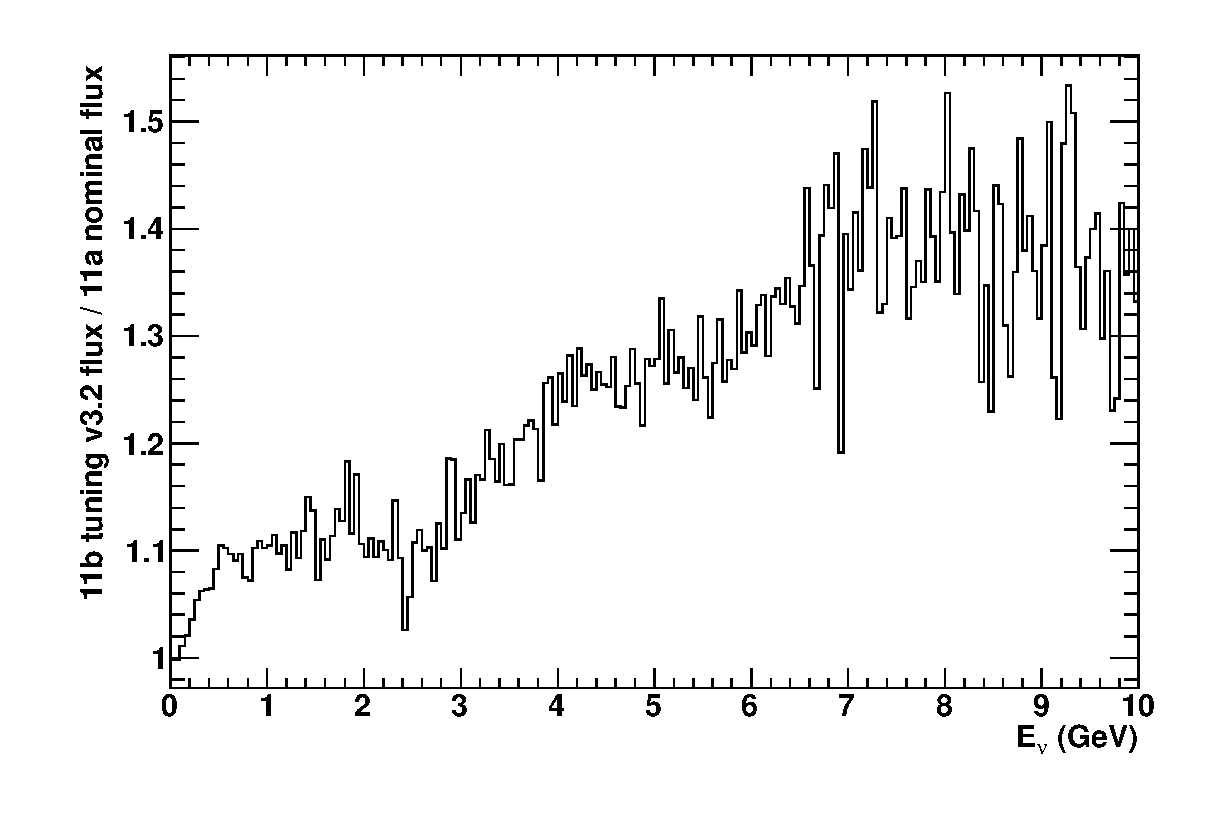
\includegraphics[width=18pc]{./images/fluxtune/fluxtune_numu}
%\caption {
%  $\nu_\mu$ 2011b\_v3.2\_run1-3c flux tuning weights applied to nominal $\nu_\mu$ and oscillated-$\nu_e$ MC templates.}
%\label{fig:na61_weights:numu}
%\end{minipage}
%\hspace{0.06\linewidth}
%\begin{minipage}[t]{0.48\linewidth}
%\center
%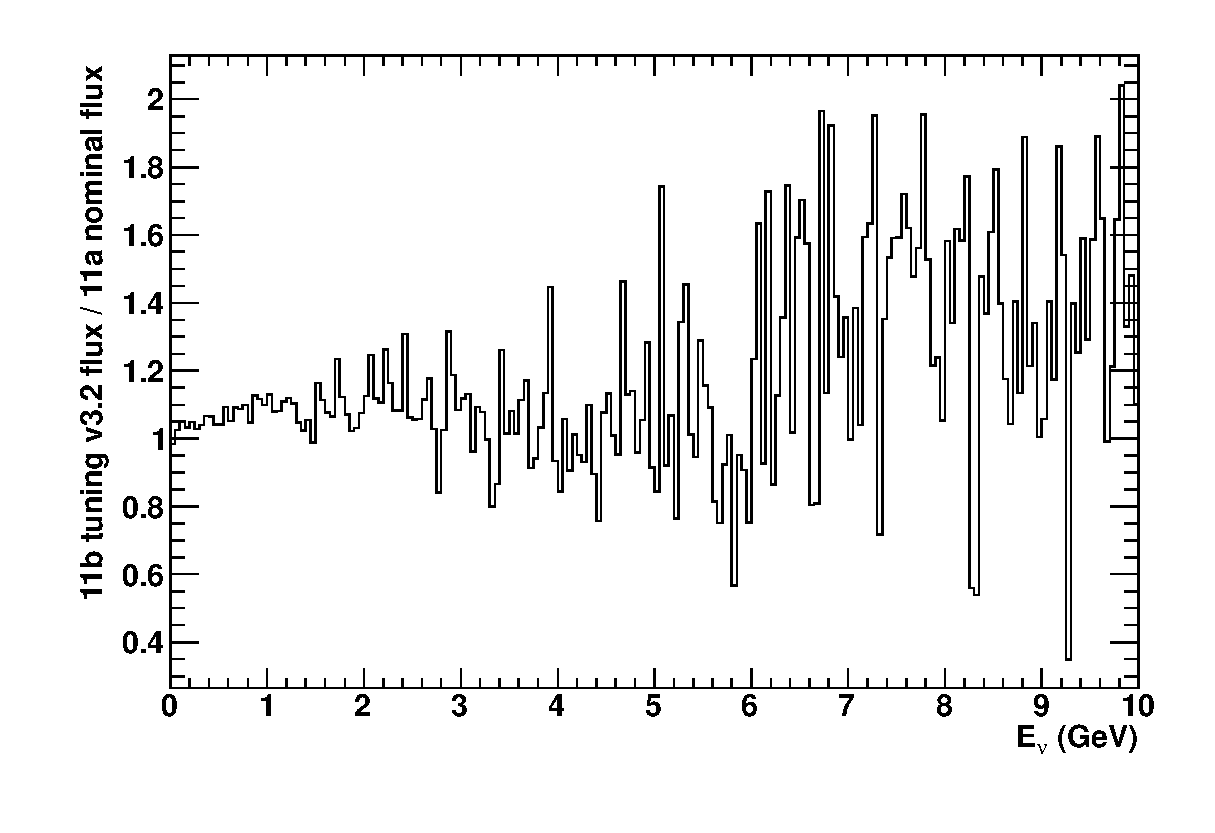
\includegraphics[width=18pc]{./images/fluxtune/fluxtune_numub}
%\caption {
%  $\bar{\nu_\mu}$ 2011b\_v3.2\_run1-3c flux tuning weights applied to nominal $\bar{\nu_\mu}$ MC templates.}
%\label{fig:na61_weights:numubar}
%\end{minipage}
%\vfill
%\begin{minipage}[t]{0.48\linewidth}
%\center
%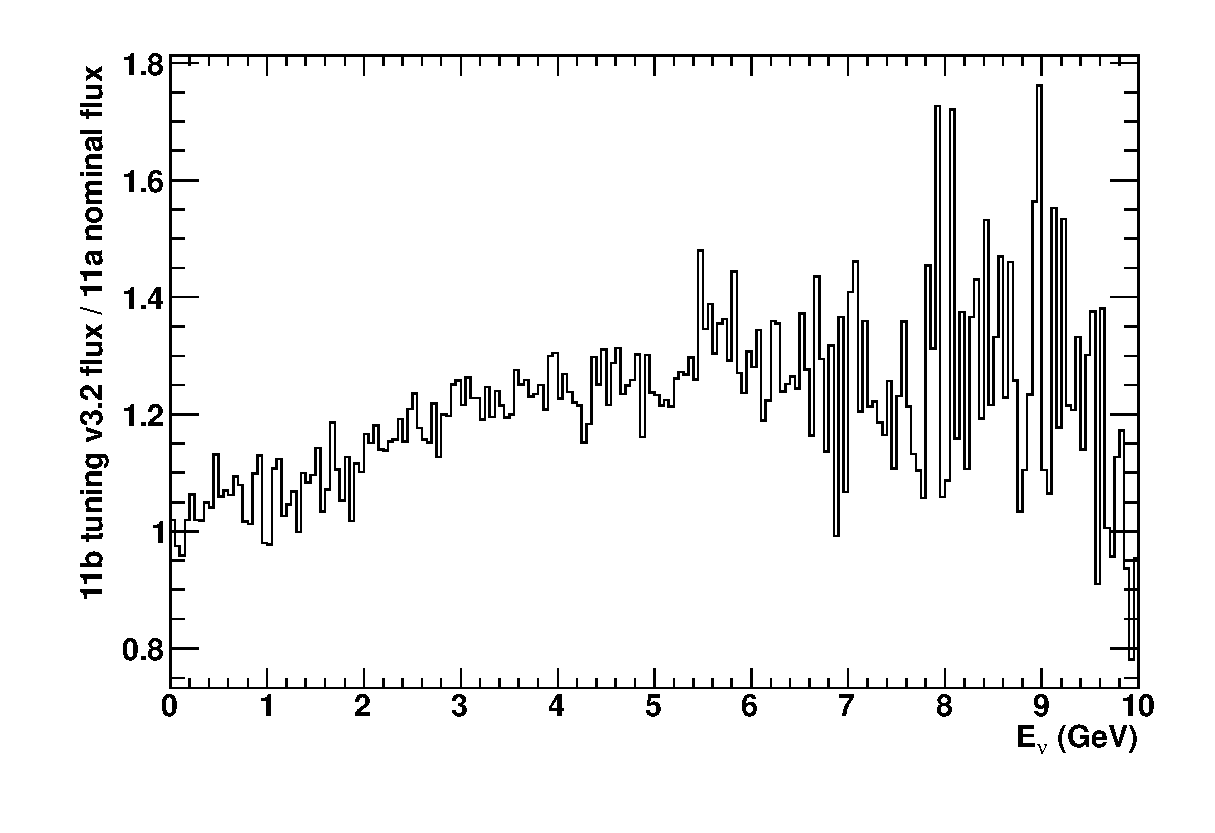
\includegraphics[width=18pc]{./images/fluxtune/fluxtune_nue}
%\caption {
%  $\nu_e$ 2011b\_v3.2\_run1-3c flux tuning weights applied to nominal $\nu_e$ MC templates.}
%\label{fig:na61_weights:nue}
%\end{minipage}
%\hspace{0.06\linewidth}
%\begin{minipage}[t]{0.48\linewidth}
%\center
%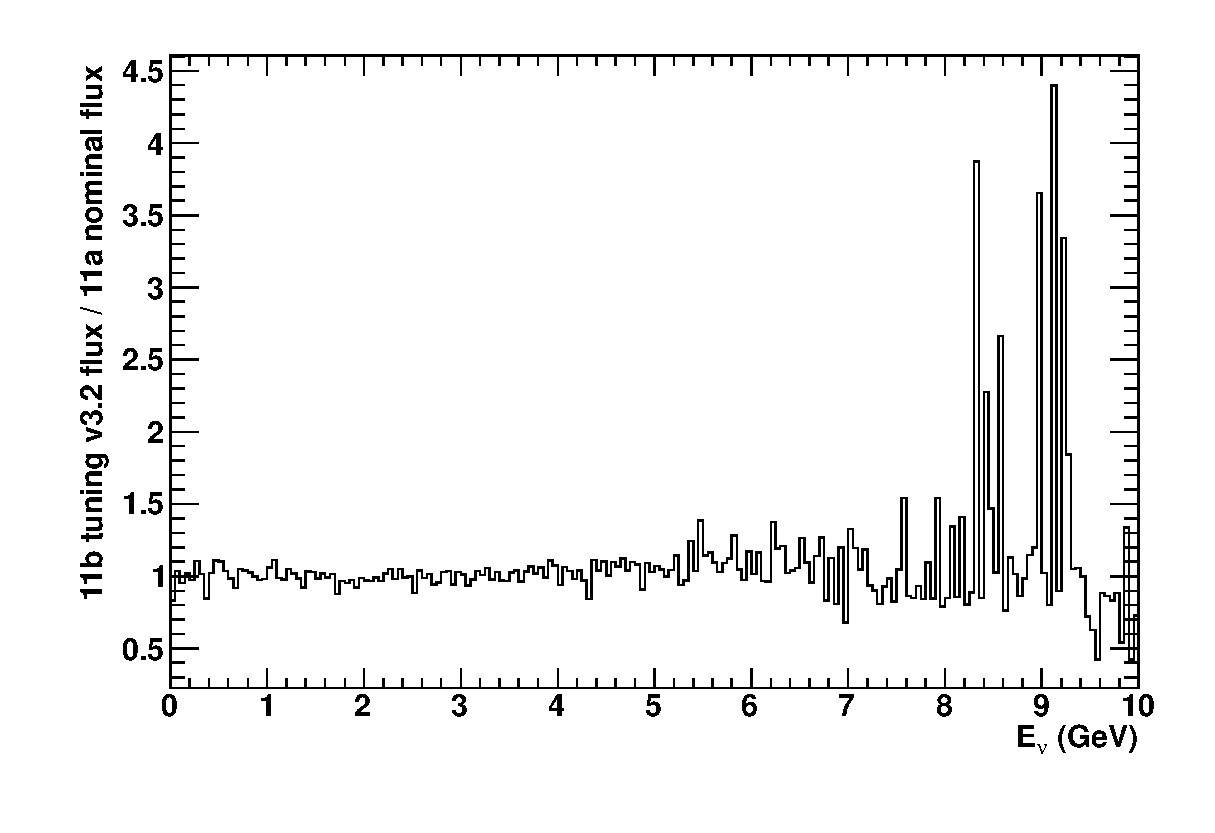
\includegraphics[width=18pc]{./images/fluxtune/fluxtune_nueb}
%\caption {
%  $\bar{\nu_e}$ 2011b\_v3.2\_run1-3c flux tuning weights applied to nominal $\bar{\nu_e}$ MC templates.}
%\label{fig:na61_weights:nuebar}
%\end{minipage}
%\end{figure*}
%

%....................................................................................................................
%....................................................................................................................

\subsection {Applying flux and cross-section (BANFF) tuning based on ND280 data}
\label{sec:banff_weights}

This analysis uses the BANFF flux and cross-section parameter tuning to reweight the NA61-tuned MC templates.
The MC templates obtained after this second reweighting will be denoted the {\em BANFF-tuned} MC templates
in this document.
Updated BANFF weights were used in this analysis with respect to the Run 1+2+3 one.

For the 2013 analyses, the ND280 $\nu_{\mu}$ group has updated the division of reconstructed ND280 CC events. 
These events are now divided into the CC0$\pi$-like, CC1$\pi$-like and CC other samples (whereas for the Run 1+2+3 analysis they were divided into CCQE-like 
and CCnonQE samples). Pion tracks are identified using ionisation energy losses in the TPC or FGD, or a pion can be identified
by the presence of a Michel electron in FGD1. The CC0$\pi$-like and CC1$\pi$-like samples have exactly 0 and 1 track consistent with
a $\pi^{+}$ respectively. The CC other sample consists of events with more than 1 track consistent with a $\pi^{+}$ or at least
one negative track or with a track consistent with an electron \cite{ND280Inputs}. The BANFF group has made a fit of these three ND280 
samples to find the best-fit values of the flux normalisation parameters and the cross-section parameters whose errors are expected to 
have some cancellation between the ND280 and SuperK, and the correlations between these parameters \cite{BANFF2013}. The postfit values of these 
parameters (taken from version 5 of the 2013 Run 1+2+3+4 BANFF fit in \verb+postfit_banff_2013_disappearance_v5.root+) are used in
turn to calculate the nominal predicted single $\mu$-like ring reconstructed energy spectrum in SuperK.
A list of BANFF parameters and their best-fit values is shown in Tab.\ \ref{tab:input_uncertainties}.

%This analysis reweights the NA61-tuned MC templates to the BANFF best-fit parameters
%\footnote{
%  The BANFF group performed its fit using an NA61-tuned flux ({\em 2011b\_v3.2\_run1-3c}),
%  the same one used for reweighting our nominal MC templates in Sec.\ \ref{sec:na61_weights}.
%}
%\footnote{
%  Reweighting the MC templates to the BANFF best-fit parameters is, in effect, a ``special''
%  systematic variation. Therefore, more details on 
%  are presented in the section detailing the systematic parameters considered in this analysis
%  (Sec.\ \ref{sec:systematics}).
%}.

The effect of the BANFF tune on the predicted reconstructed energy spectrum of
single $\mu$-like ring events is discussed in Sec.\ \ref{sec:nominal_and_tuned_predictions} (see 
Figs.\ \ref{fig:nsk_vs_osc_params_effect_of_banff_tune} and \ref{fig:1Rmu_spectrum_w_and_wo_banff_weights}, and
Tabs.\ \ref{tab:nsk_nominal_x3_no_osc} and \ref{tab:nsk_nominal_x3_default_osc}).

%....................................................................................................................
%....................................................................................................................

\subsection{Applying neutrino oscillations}
\label{sec:applying_oscillations}

Oscillation probabilities are computed in a 3-flavour framework including matter effects in constant-density matter
(assuming an Earth crust density of 2.6 g/cm$^{3}$).
Custom oscillation probability calculation code was developed within the {\em VALOR} analysis framework.
Details and estimates of the numerical accuracy of this code were first presented in \cite{OurRun12DisappAnalysis3Flavour},
and is also shown in Appendix A of \cite{OurRun123DisappAnalysis3Flavour}.
Comparisons between the {\em VALOR} oscillation probability calculation code and Prob3++ \cite{Prob3}, 
which is typically used by the alternative T2K oscillation analyses, are shown in Appendix B of \cite{OurRun123DisappAnalysis3Flavour}.

Oscillations are applied as a function of true energy to the 
  $\nu_{\mu}$ CCQE,
  $\nu_{\mu}$ CC1$\pi$, 
  $\nu_{\mu}$ CC coherent, 
  $\nu_{\mu}$ CC other, 
  $\bar{\nu}_{\mu}$ CCQE, 
  $\bar{\nu}_{\mu}$ CC1$\pi$, 
  $\bar{\nu}_{\mu}$ CC coherent, 
  $\bar{\nu}_{\mu}$ CC other, 
  $\nu_{e}$ CCQE, 
  $\nu_{e}$ CC1$\pi$,
  $\nu_{e}$ CC coherent,
  $\nu_{e}$ CC other,
  $\bar{\nu}_{e}$ CCQE, 
  $\bar{\nu}_{e}$ CC1$\pi$,
  $\bar{\nu}_{e}$ CC coherent,
  $\bar{\nu}_{e}$ CC other,
  oscillated $\nu_{\mu} \rightarrow \nu_{e}$ CCQE,
  oscillated $\nu_{\mu} \rightarrow \nu_{e}$ CC1$\pi$,
  oscillated $\nu_{\mu} \rightarrow \nu_{e}$ CC coherent,
  oscillated $\nu_{\mu} \rightarrow \nu_{e}$ CC other,
  oscillated $\nu_{e} \rightarrow \nu_{\mu}$ CCQE,
  oscillated $\nu_{e} \rightarrow \nu_{\mu}$ CC1$\pi$,
  oscillated $\nu_{e} \rightarrow \nu_{\mu}$ CC coherent and
  oscillated $\nu_{e} \rightarrow \nu_{\mu}$ CC other
MC templates.

The MC templates constructed from the unoscillated MC samples are weighted 
with the corresponding survival probability:
The $\nu_{\mu}$ templates are weighted with P($\nu_{\mu}\rightarrow\nu_{\mu}$),
the $\bar{\nu}_{\mu}$ templates with P($\bar{\nu}_{\mu}\rightarrow\bar{\nu}_{\mu}$),
the $\nu_{e}$ templates with P($\nu_{e}\rightarrow\nu_{e}$) and
the $\bar{\nu}_{e}$ templates with P($\bar{\nu}_{e}\rightarrow\bar{\nu}_{e}$).
The MC templates made from the oscillated $\nu_{\mu} \rightarrow \nu_{e}$ MC sample are weighted with 
P($\nu_{\mu}\rightarrow\nu_{e}$) (the sample was generated assuming 100\% of 
$\nu_{\mu}$ transform to $\nu_{e}$), 
while the MC templates made from the oscillated  $\nu_{e} \rightarrow \nu_{\mu}$ MC sample are weighted with
P($\nu_{e}\rightarrow\nu_{\mu}$).

In the standard 3-flavour oscillation framework,
oscillations of $\nu_{e}$ and $\nu_{\mu}$ can yield $\nu_{\tau}$, while
oscillations of $\bar{\nu}_{e}$ and $\bar{\nu}_{\mu}$ can yield $\bar{\nu}_{\tau}$.
In this analysis, we neglect contributions from $\nu_{\tau}$-CC and $\bar{\nu}_{\tau}$-CC as their
energy threshold is around 3.5 GeV and their effect is negligible\footnote{
A back-of-the-envelope calculation can be found in the replies to
comments and revision history document of
\cite{OurRun123DisappAnalysis3Flavour} that gives $\ll 1\%$ $\nu_\tau$
contamination in the 1-ring $\mu$-like SuperK sample. A SuperK MC study is required
to determine whether the SuperK efficiency assumptions made there are valid.
  }.
Accordingly, this analysis uses no $\nu_{\tau}$-CC and $\bar{\nu}_{\tau}$-CC MC templates
(and, in fact, no $\nu_{\tau}$ and $\bar{\nu}_{\tau}$ SuperK MC samples are available).

It should be emphasized here that
the $\nu_{\mu}$ NC MC templates for a mode $m$ are proxies for the
NC MC templates for the mixture of $\nu_{e}$+$\nu_{\mu}$+$\nu_{\tau}$ resulting from
3-flavour $\nu_{\mu}$ oscillations for that mode $m$. The same applies to the $\bar{\nu}_{\mu}$, $\nu_{e}$ and $\bar{\nu}_{e}$ NC MC templates.
These NC MC templates are unchanged under standard 3-flavour oscillations.% (see also Sec.\ \ref{sec:}).

Also it should be noted that there are no explicit NC MC templates made from the oscillated $\nu_{e}$ sample.
If they were used, the oscillated $\nu_{e}$ (i.e.\ $\nu_{e}$ coming from $\nu_{\mu}$ oscillations) would be double counted
since they are already included in the $\nu_{\mu}$ NC MC templates.

The same oscillation parameters are used for neutrinos and antineutrinos.
% The same oscillation parameters are used for $\nu_{\mu}$, $\bar{\nu}_{\mu}$, $\nu_{e}$ and $\bar{\nu}_{e}$ 
% oscillations, and these are $\sin^{2}{\theta_{23}}$, $|\Delta m^{2}_{32}|$ (normal hierarchy) or $|\Delta m^{2}_{31}|$ (inverted hierarchy),
% $\sin^{2}{\theta_{13}}$, $\sin^{2}{\theta_{12}}$, $\Delta m^{2}_{21}$ and $\delta_{CP}$.

%....................................................................................................................

\subsection {Predictions of nominal and tuned-MC single $\mu$-like ring spectra}
\label{sec:nominal_and_tuned_predictions}

In this section, we present the expected numbers of events and single $\mu$-like ring
reconstructed energy spectra in SuperK for various oscillation scenarios.
We also present estimates of the effect of the NA61 and BANFF tunings and of assumptions made in the 3-flavour
neutrino oscillation framework used in this analysis.
Unless explicitly stated otherwise, the normal hierarchy is assumed, $\delta_{CP}$ = 0,
and the values shown in Tab.\ \ref{tab:pdg2012non23}
are used for $\sin^{2}\theta_{13}$, $\sin^{2}\theta_{12}$ and $\Delta m^{2}_{21}$.
All plots were generated for an integrated exposure of 6.5700$\times$10$^{20}$ POT.

The expected number of single $\mu$-like ring events is shown in Fig.\ \ref{fig:nsk_vs_osc_params_tuned_mc}
as a function of the oscillation parameters $\sin^{2}{\theta_{23}}$ and $|\Delta m^{2}_{32}|$.
The expected number of events ranges from a minimum of $\sim$122,
to more than $\sim$146 for oscillation parameter values still within the T2K Run 1+2+3 90\% CL region.
This illustrates the great sensitivity of the T2K $\nu_{\mu}$-disappearance analysis in measuring $\sin^{2}{\theta_{23}}$
with the Run 1+2+3+4 data.

Predicted single $\mu$-like ring SuperK reconstructed energy spectra are shown in
Fig. \ref{fig:1Rmu_spectrum_and_components_no_osc} for no oscillations, and in
Fig. \ref{fig:1Rmu_spectrum_and_components_default_osc} for oscillations
with $\sin^{2}\theta_{23}$ = 0.5 and $|\Delta m^{2}_{32}|$ = 2.4$\times$10$^{-3}$ eV$^{2}$/c$^{4}$.

A MC tune derived using NA61 data is applied to the nominal MC templates, and another tune derived using the ND280 data is 
applied to the NA61-tuned templates as described in Secs.\ \ref{sec:na61_weights} and \ref{sec:banff_weights}.
The fractional difference in the expected number of single $\mu$-like ring events when switching from the nominal MC to the
NA61-tuned MC templates is shown in Fig.\ \ref{fig:nsk_vs_osc_params_effect_of_na61_tune} as a function of the oscillation
parameters $\sin^{2}{\theta_{23}}$ and $|\Delta m^{2}_{32}|$.
In Fig. \ref{fig:nsk_vs_osc_params_effect_of_banff_tune} is shown the fractional difference in the expected number of
single-ring $\mu$-like events when switching from the NA61-tuned MC templates to the BANFF-tuned MC templates.
From these figures it can be seen that, for oscillation parameters in the T2K Run 1+2+3 90\% confidence region,
$\sim$12.4-13.0\% more single-ring $\mu$-like events are obtained with
the NA61-tuned MC than with the nominal MC.
In the same part of the parameter space, $\sim$7.0-8.2\% fewer events are expected with the BANFF-tuned MC
than with the NA61-tuned MC.
The effects of the NA61 and BANFF tunes on the total expected number of single-ring $\mu$-like events
and on the numbers in each of the 32 component interaction modes are shown in
Tab.\ \ref{tab:nsk_nominal_x3_no_osc} for no oscillations, and in
Tab.\ \ref{tab:nsk_nominal_x3_default_osc} for oscillations
with $\sin^{2}\theta_{23}$ = 0.5 and $|\Delta m^{2}_{32}|$ = 2.4$\times$10$^{-3}$ eV$^{2}$/c$^{4}$.
Finally, the effects of the NA61 and BANFF tunes on the reconstructed energy spectrum of
single $\mu$-like ring events are shown in Figs.\
\ref{fig:1Rmu_spectrum_w_and_wo_na61_weights} and
\ref{fig:1Rmu_spectrum_w_and_wo_banff_weights} respectively.
In each case, spectra are shown for both no oscillations and for
oscillations with $\sin^{2}\theta_{23}$ = 0.5 and $|\Delta m^{2}_{32}|$ = 2.4$\times$10$^{-3}$ eV$^{2}$/c$^{4}$.
Also shown are the ratio of flux-tuned spectrum to nominal spectrum, and
BANFF-tuned spectrum to flux-tuned spectrum in Figs.\
\ref{fig:1Rmu_spectrum_w_and_wo_na61_weights} and
\ref{fig:1Rmu_spectrum_w_and_wo_banff_weights} respectively.

%
%When making a fit to obtain the best-fit values of
%$\sin^{2}\theta_{23}$ and $|\Delta m^{2}_{32}|$,
%$\delta_{CP}$ is fixed to 0,
%and we also fit
%other oscillation parameters ($\sin^2\theta_{13}$, $\sin^2\theta_{12}$, $\Delta m^2_{21}$)
%using the errors listed in Tab. \ref{tab:pdg2012non23} as constraints.
%The best-fit values and constraints come from the 2012 PDG \cite{PDG2012} for
%$\sin^2\theta_{13}$ and $\Delta m^2_{21}$, and from a global fit \cite{FogliLisi}
%for $\sin^2\theta_{12}$, so as to be consistent with the latest $\nu_e$ appearance fits
%\cite{2013nuenergy,2013nueptheta}.
%
%\begin{table}
%\centering
%\begin{tabular}{| c | c | c | }
%\hline
%Parameter                  &  Best-fit                                    & 1$\sigma$ error  \\
%\hline
%$\Delta m_{21}^{2}$      &  7.5 $\times$ 10$^{-5}$ eV$^{2}$/c$^{4}$     & $\sim$2.7\% \\
%$\sin^{2}(\theta_{12})$  &  0.306                                       & $\sim$5.9\% \\
%$\sin^{2}(\theta_{13})$  &  0.0251                                      & $\sim$13.9\% \\
%$\delta_{CP}$            &  0                                           & $\pi$ \\
%\hline
%\end{tabular}
%\caption{
%  The best-fit values and 1$\sigma$ range for the measured \emph{non-23-sector} oscillation parameters \cite{PDG2012,FogliLisi}.
%}
%\label{tab:pdg2012non23}
%\end{table}
%
%The maximum possible effect of this assumption on the expected number of single-ring $\mu$-like events is shown
%in Fig.\ \ref{fig:nsk_vs_osc_params_tuned_mc_effect_of_non23}.
%In each bin of $\sin^{2}{\theta_{23}}$ and $|\Delta m^{2}_{32}|$,
%a large number of toy MC experiments was generated with randomized values of the \emph{non-23-sector} parameters.
%The random values of $\sin^{2}\theta_{13}$, $\sin^{2}\theta_{12}$ and $\Delta m^{2}_{21}$ were drawn from
%Gaussian distributions with means equal to the 1$\sigma$
%errors, while the values of $\delta_{CP}$ were drawn from a uniform distribution between -$\pi$ and +$\pi$.
%These four \emph{non-23-sector} parameters were taken to be uncorrelated.
%The maximum fractional deviation from the default case was recorded and plotted
%in Fig.\ \ref{fig:nsk_vs_osc_params_tuned_mc_effect_of_non23}.
%From this figure, it can be seen that the maximum effect of the \emph{non-23-sector} oscillation parameters
%is of the order of $\sim$1.7\% in the part of
%the parameter space covered by the T2K Run 1+2+3 90\% confidence region.
%
%All the results in this analysis assume the normal mass hierarchy,
%unless explicitly stated.
%The effect of this assumption on the expected number of single-ring $\mu$-like events
%is shown in Fig.\ \ref{fig:nsk_vs_osc_params_tuned_mc_effect_of_hierarchy}
%as a function of the oscillation parameters $\sin^{2}{\theta_{23}}$ and $|\Delta m^{2}_{32}|$.
%The effect is large and potentially misleading, and some clarifications are in order.
%This analysis can assume a given hierarchy without loss of generality of its results.
%Fig.\ \ref{fig:nsk_vs_osc_params_tuned_mc_effect_of_hierarchy} reveals that $|\Delta m^{2}_{32}|$ is a poor
%choice as the atmospheric mass-squared difference when both mass hierarchies need to be considered,
%since $|\Delta m^{2}_{32}|$ is the largest mass-squared difference for the inverted hierarchy
%but the second-largest for the normal hierarchy.
%The large difference shown in Fig.\ \ref{fig:nsk_vs_osc_params_tuned_mc_effect_of_hierarchy}
%is caused by the change in value of $\Delta m^{2}_{31}$ when switching from the
%normal to inverted hierarchy.
%
%Other choices exist for the atmospheric mass-squared difference, and these are explained in Sec.\
%2.3 in \cite{OurRun12DisappAnalysis3Flavour}. An example of an alternative choice is shown vividly in
%Fig.\ 5 in \cite{OurRun12DisappAnalysis3Flavour}; this technical note describes a repeat, in a 3-flavour
%framework, of our official Run 1+2 disappearance analysis \cite{OurRun12DisappAnalysis} which was originally
%performed in a 2-flavour framework.
%

%...........
%
% nsk
%
\begin{figure*}[htb]
\center
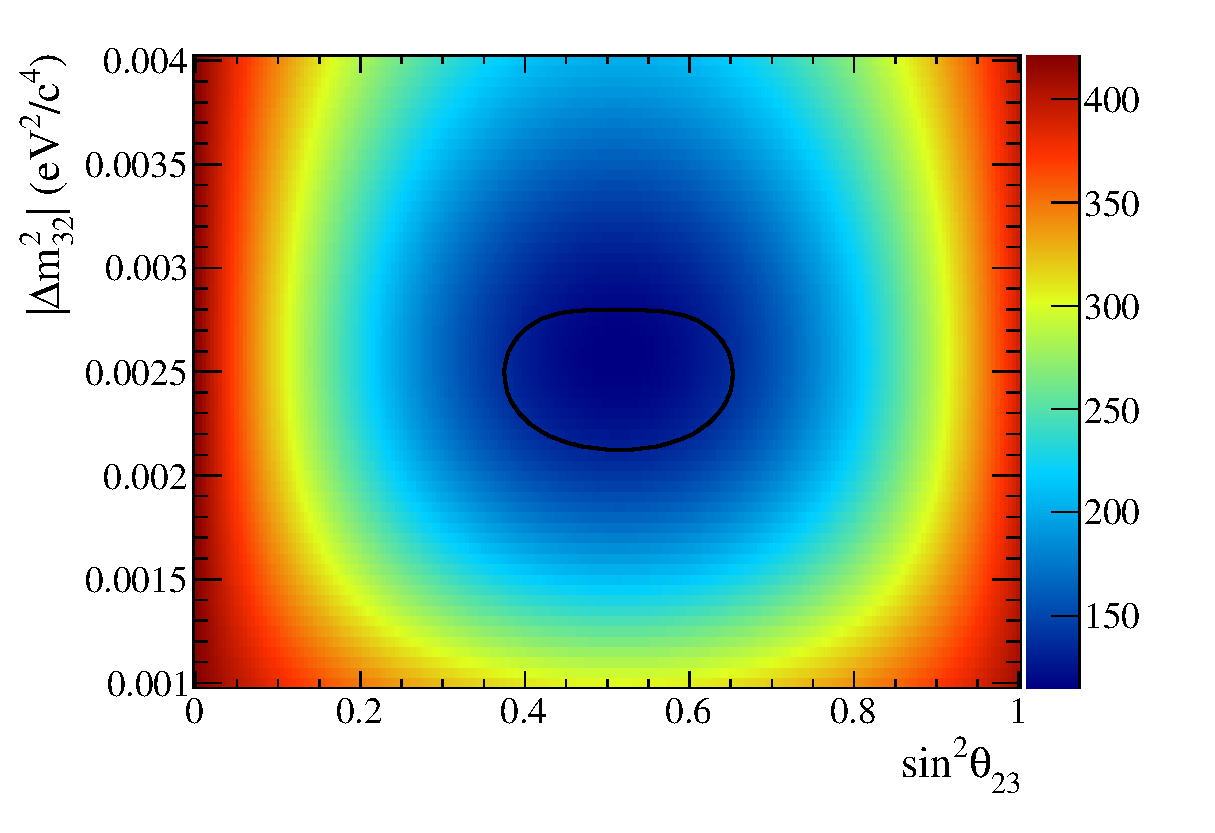
\includegraphics[width=32pc]{./images/spectrum_predictions/nsk_nominalbanff}
\caption {
  Predicted number of 1 $\mu$-like ring events,
  as a function of $\sin^{2}\theta_{23}$ and $|\Delta m^{2}_{32}|$,
  for an exposure of 6.5700$\times$10$^{20}$ POT.
  The numbers of events were calculated using the BANFF-tuned MC templates.
  $\sin^{2}\theta_{13}$, $\sin^{2}\theta_{12}$ and $\Delta m^{2}_{21}$ have the values shown in Tab.\ \ref{tab:pdg2012non23} and $\delta_{CP}$=0.
  The numbers shown were generated assuming the normal hierarchy.
  The T2K Run 1+2+3 90\% C.L.\ region is superimposed for reference.
}
\label{fig:nsk_vs_osc_params_tuned_mc}
\end{figure*}

%...........
%
% spectra, various osc scenarios
%
\begin{figure*}[htb]
\begin{minipage}[t]{0.48\linewidth}
\center
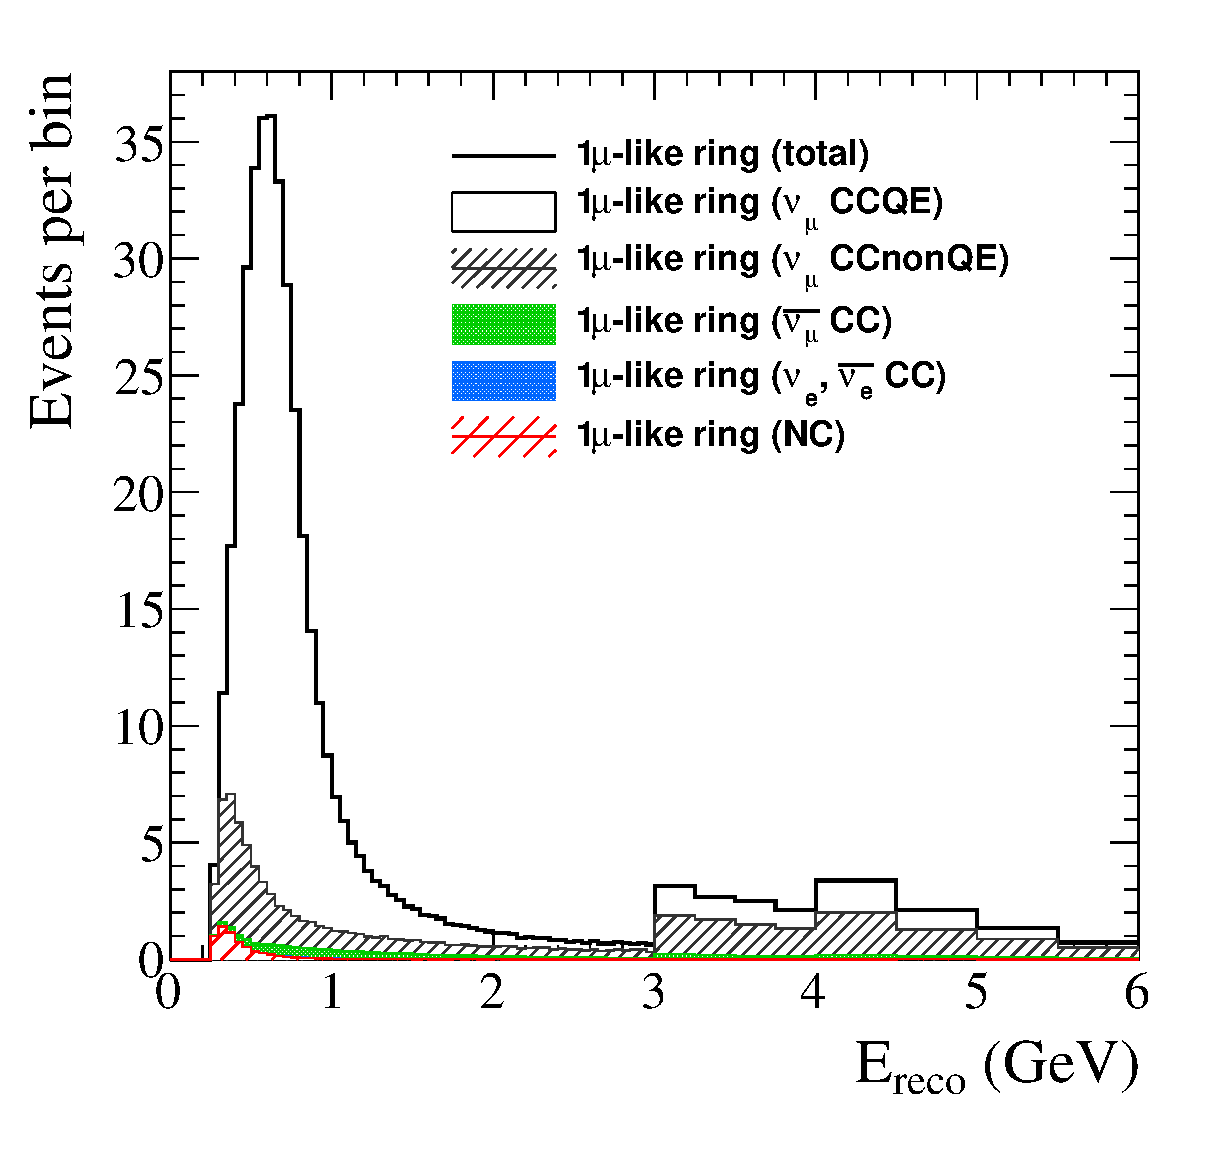
\includegraphics[width=20pc]{./images/spectrum_predictions/spectrum_breakdown_notoscillated_normal}
\caption {
Predicted reconstructed-energy spectrum of 1 $\mu$-like ring events,
and contributions from various true neutrino reaction modes,
for no oscillations and
for an exposure of 6.5700$\times$10$^{20}$ POT.
The 32 components of the spectrum are calculated separately in the actual analysis,
but, for this plot, are grouped into just 5 categories:
$\nu_{\mu}$ CCQE, $\nu_{\mu}$ CCnonQE, $\bar{\nu}_{\mu}$ CC, $\nu_{e}$/$\bar{\nu}_{e}$ CC and NC.
The spectrum was generated using the BANFF-tuned MC templates.
}
\label{fig:1Rmu_spectrum_and_components_no_osc}
\end{minipage}
\hspace{0.06\linewidth}
\begin{minipage}[t]{0.48\linewidth}
\center
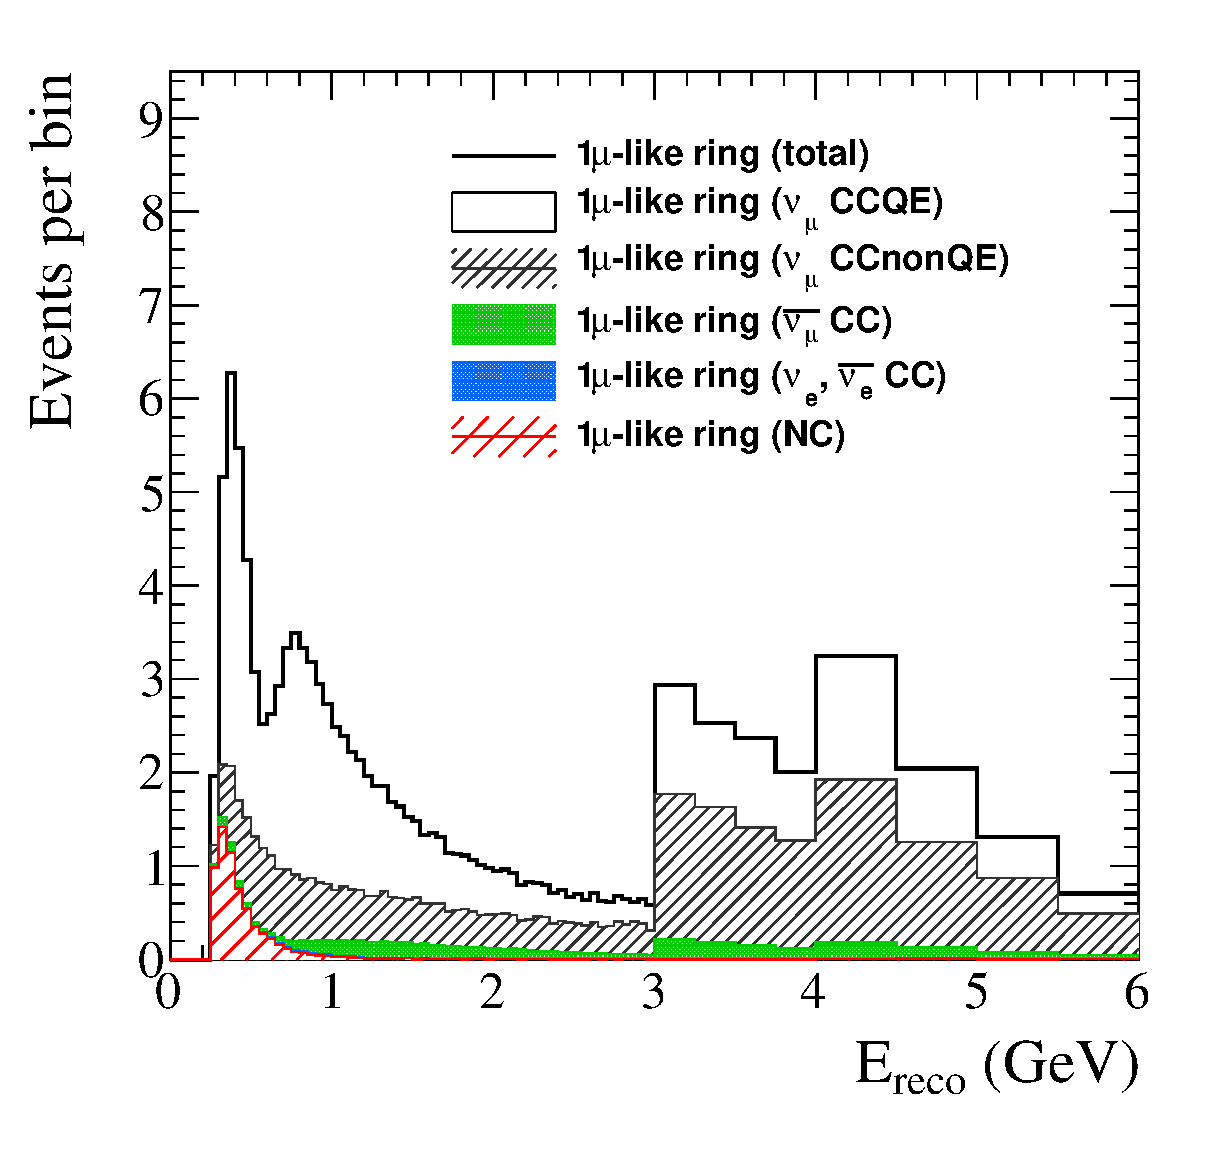
\includegraphics[width=20pc]{./images/spectrum_predictions/spectrum_breakdown_oscillated_normal}
\caption {
Predicted reconstructed-energy spectrum of 1 $\mu$-like ring events,
and contributions from various true neutrino reaction modes,
for oscillations with $\sin^{2}\theta_{23}$=0.5 and $|\Delta m^{2}_{32}|$=2.4$\times10^{-3}$ eV$^{2}$/c$^{4}$
and for an exposure of 6.5700$\times$10$^{20}$ POT.
The spectrum was generated using the BANFF-tuned MC templates.
$\sin^{2}\theta_{13}$, $\sin^{2}\theta_{12}$ and $\Delta m^{2}_{21}$ have the values shown in Tab.\ \ref{tab:pdg2012non23} and $\delta_{CP}$=0.
The spectrum shown was generated assuming the normal hierarchy.
Note that the vertical axis is zoomed in by a factor of 4 compared with Fig.\ \ref{fig:1Rmu_spectrum_and_components_no_osc}.
}
\label{fig:1Rmu_spectrum_and_components_default_osc}
\end{minipage}
\end{figure*}

%...........
%
% effect of tunes on nsk
%
\begin{figure*}[htb]
\begin{minipage}[t]{0.48\linewidth}
\center
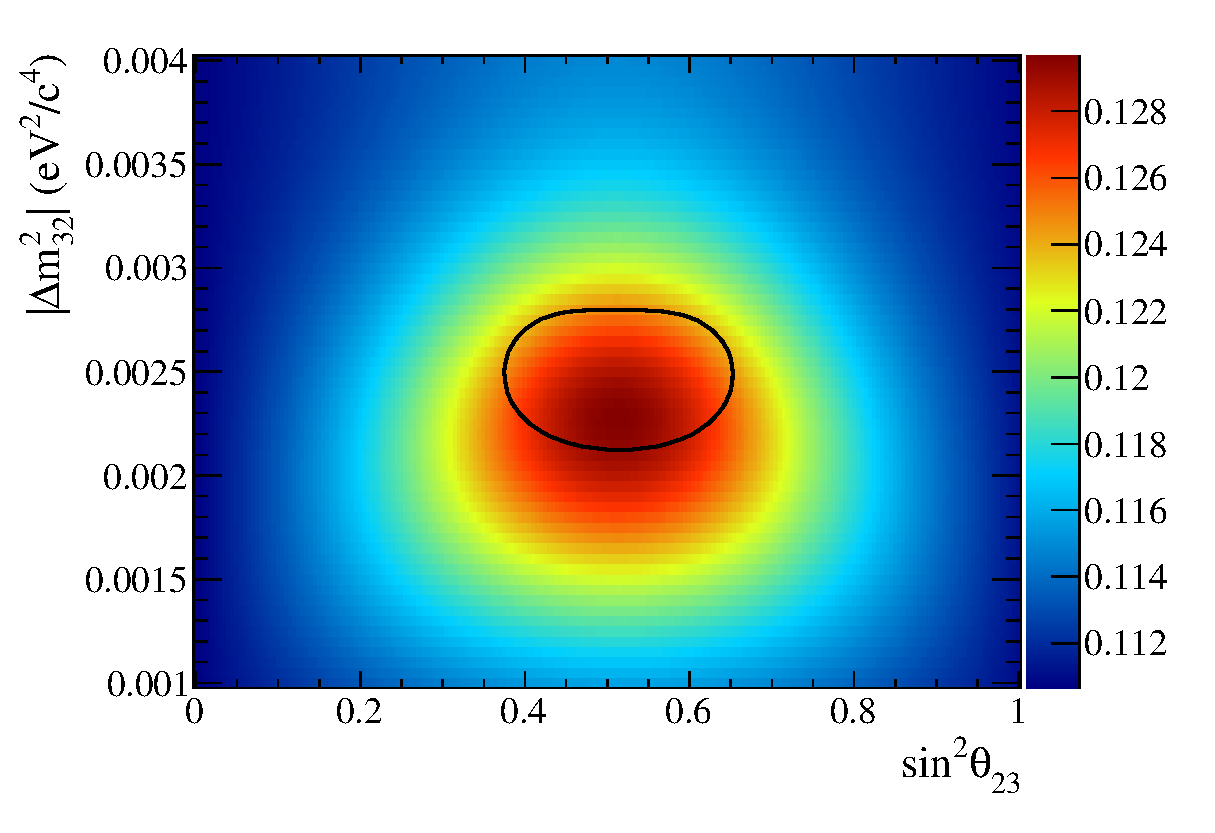
\includegraphics[width=18pc]{./images/spectrum_predictions/nsk_diff_nomflux}
\caption {
  Fractional difference in the predicted number of 1 $\mu$-like ring events
  as a result of applying the NA61 flux tuning to the nominal MC templates.
  These numbers are shown as a function of $\sin^{2}\theta_{23}$ and $|\Delta m^{2}_{32}|$
  for an exposure of 6.5700$\times$10$^{20}$ POT.
  $\sin^{2}\theta_{13}$, $\sin^{2}\theta_{12}$ and $\Delta m^{2}_{21}$ have the values shown in Tab.\ \ref{tab:pdg2012non23} and $\delta_{CP}$=0.
  The numbers shown were generated assuming the normal hierarchy.
  The T2K Run 1+2+3 90\% CL region is superimposed for reference.
}
\label{fig:nsk_vs_osc_params_effect_of_na61_tune}
\end{minipage}
\hspace{0.06\linewidth}
\begin{minipage}[t]{0.48\linewidth}
\center
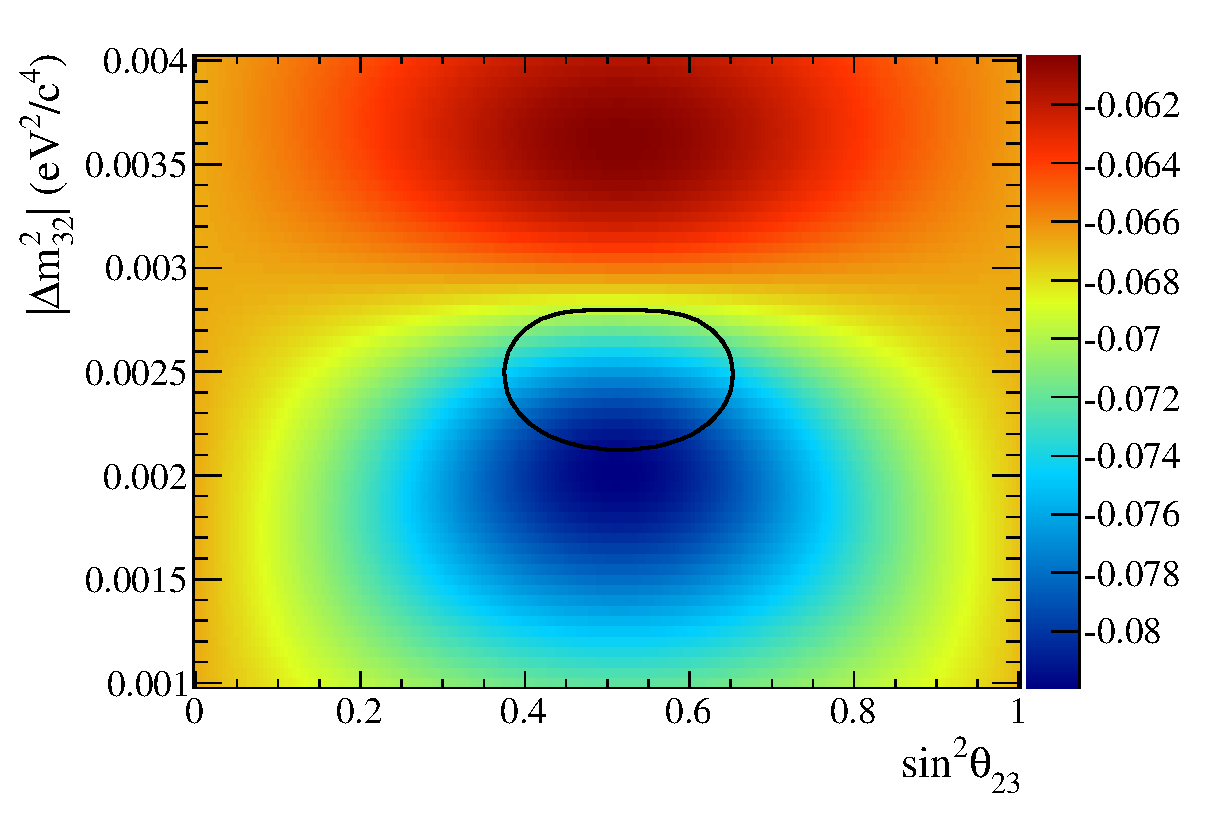
\includegraphics[width=18pc]{./images/spectrum_predictions/nsk_diff_tunflux}
\caption {
  Fractional difference in the predicted number of 1 $\mu$-like ring events
  as a result of applying the BANFF flux and cross-section tuning to the NA61 flux tuned MC templates.
  These numbers are shown as a function of $\sin^{2}\theta_{23}$ and $|\Delta m^{2}_{32}|$ and
  for an exposure of 6.5700$\times$10$^{20}$ POT.
  $\sin^{2}\theta_{13}$, $\sin^{2}\theta_{12}$ and $\Delta m^{2}_{21}$ have the values shown in Tab.\ \ref{tab:pdg2012non23} and $\delta_{CP}$=0.
  The numbers shown were generated assuming the normal hierarchy.
  The T2K Run 1+2+3 90\% CL region is superimposed for reference.
}
\label{fig:nsk_vs_osc_params_effect_of_banff_tune}
\end{minipage}
\end{figure*}

%...........
%
% tables showing the effect of tunes on nsk and nsk components
%

\begin{table}
\centering
\begin{tabular}{| c |  D{.}{.}{-1} |  D{.}{.}{-1} |  D{.}{.}{-1} | }
\hline
         & \multicolumn{1}{c|}{$N_{SK}$}     & \multicolumn{1}{c|}{$N_{SK}$}          & \multicolumn{1}{c|}{$N_{SK}$}          \\ 
         & \multicolumn{1}{c|}{(nominal MC)} & \multicolumn{1}{c|}{(NA61-tuned MC)}  & \multicolumn{1}{c|}{(BANFF-tuned MC)}  \\ 
\hline
Total & 418.131220 & 464.272533 & 445.980111 \\ 
\hline
$\nu_\mu$ CCQE & 332.238749 & 367.166655 & 351.657098 \\ 
$\nu_\mu$ CC 1$\pi$ & 56.190220 & 63.533041 & 62.227879 \\ 
$\nu_\mu$ CC coherent & 1.896444 & 2.136085 & 2.108162 \\ 
$\nu_\mu$ CC other & 7.963009 & 9.600253 & 9.615971 \\ 
$\nu_\mu$/$\nu_\tau$ NC 1$\pi^{+/-}$ & 3.403911 & 3.888131 & 2.934821 \\ 
$\nu_\mu$/$\nu_\tau$ NC other & 2.912186 & 3.428374 & 3.228957 \\ 
Osc. $\nu_\mu$ CCQE & 0.000000 & 0.000000 & 0.000000 \\ 
Osc. $\nu_\mu$ CC 1$\pi$ & 0.000000 & 0.000000 & 0.000000 \\ 
Osc. $\nu_\mu$ CC coherent & 0.000000 & 0.000000 & 0.000000 \\ 
Osc. $\nu_\mu$ CC other & 0.000000 & 0.000000 & 0.000000 \\ 
$\bar{\nu_\mu}$ CCQE & 9.008088 & 9.664244 & 9.521964 \\ 
$\bar{\nu_\mu}$ CC 1$\pi$ & 2.909354 & 3.114170 & 3.061538 \\ 
$\bar{\nu_\mu}$ CC coherent & 0.428081 & 0.458785 & 0.466122 \\ 
$\bar{\nu_\mu}$ CC other & 0.519092 & 0.553722 & 0.548210 \\ 
$\bar{\nu_\mu}$/$\bar{\nu_\tau}$ NC 1$\pi^{+/-}$ & 0.188316 & 0.203257 & 0.143433 \\ 
$\bar{\nu_\mu}$/$\bar{\nu_\tau}$ NC other & 0.176427 & 0.188866 & 0.175090 \\ 
$\nu_e$ CCQE & 0.035370 & 0.038166 & 0.037333 \\ 
$\nu_e$ CC 1$\pi$ & 0.021574 & 0.023840 & 0.023994 \\ 
$\nu_e$ CC coherent & 0.001057 & 0.001158 & 0.001158 \\ 
$\nu_e$ CC other & 0.005812 & 0.006914 & 0.006795 \\ 
$\nu_e$ NC 1$\pi^{+/-}$ & 0.091432 & 0.105093 & 0.075133 \\ 
$\nu_e$ NC other & 0.112184 & 0.131680 & 0.121606 \\ 
$\bar{\nu_e}$ CCQE & 0.002174 & 0.002187 & 0.002102 \\ 
$\bar{\nu_e}$ CC 1$\pi$ & 0.001376 & 0.001385 & 0.001345 \\ 
$\bar{\nu_e}$ CC coherent & 0.000135 & 0.000137 & 0.000137 \\ 
$\bar{\nu_e}$ CC other & 0.000442 & 0.000446 & 0.000432 \\ 
$\bar{\nu_e}$ NC 1$\pi^{+/-}$ & 0.012254 & 0.012354 & 0.008390 \\ 
$\bar{\nu_e}$ NC other & 0.013532 & 0.013592 & 0.012439 \\ 
Osc. $\nu_e$ CCQE & 0.000000 & 0.000000 & 0.000000 \\ 
Osc. $\nu_e$ CC 1$\pi$ & 0.000000 & 0.000000 & 0.000000 \\ 
Osc. $\nu_e$ CC coherent & 0.000000 & 0.000000 & 0.000000 \\ 
Osc. $\nu_e$ CC other & 0.000000 & 0.000000 & 0.000000 \\ 
\hline
\end{tabular}
\caption{
  Calculated numbers of 1-ring $\mu$-like events without oscillations using the nominal MC templates, the
  NA61-tuned MC templates and the BANFF-tuned MC templates.
  The total numbers of events and the numbers of events from each mode considered in this analysis are shown.
  These numbers were calculated for an exposure of 6.5700$\times$10$^{20}$ POT.
}
\label{tab:nsk_nominal_x3_no_osc}
\end{table}


\begin{table}
\centering
\begin{tabular}{| c |  D{.}{.}{-1} |  D{.}{.}{-1} |  D{.}{.}{-1} | }
\hline
         & \multicolumn{1}{c|}{$N_{SK}$}     & \multicolumn{1}{c|}{$N_{SK}$}          & \multicolumn{1}{c|}{$N_{SK}$}          \\ 
         & \multicolumn{1}{c|}{(nominal MC)} & \multicolumn{1}{c|}{(NA61-tuned MC)}  & \multicolumn{1}{c|}{(BANFF-tuned MC)}  \\ 
\hline
Total & 116.283270 & 131.048525 & 124.981851 \\ 
\hline
$\nu_\mu$ CCQE & 66.133875 & 73.447588 & 70.993870 \\ 
$\nu_\mu$ CC 1$\pi$ & 27.733771 & 31.941870 & 29.795498 \\ 
$\nu_\mu$ CC coherent & 0.777452 & 0.896207 & 0.908178 \\ 
$\nu_\mu$ CC other & 7.072249 & 8.586001 & 8.597815 \\ 
$\nu_\mu$/$\nu_\tau$ NC 1$\pi^{+/-}$ & 3.403911 & 3.888131 & 2.934821 \\ 
$\nu_\mu$/$\nu_\tau$ NC other & 2.912186 & 3.428374 & 3.228957 \\ 
Osc. $\nu_\mu$ CCQE & 0.117417 & 0.129898 & 0.127451 \\ 
Osc. $\nu_\mu$ CC 1$\pi$ & 0.027388 & 0.030497 & 0.030950 \\ 
Osc. $\nu_\mu$ CC coherent & 0.000821 & 0.000913 & 0.000913 \\ 
Osc. $\nu_\mu$ CC other & 0.002344 & 0.002648 & 0.002609 \\ 
$\bar{\nu_\mu}$ CCQE & 4.428977 & 4.745506 & 4.621408 \\ 
$\bar{\nu_\mu}$ CC 1$\pi$ & 2.080140 & 2.219962 & 2.132869 \\ 
$\bar{\nu_\mu}$ CC coherent & 0.228753 & 0.244521 & 0.248227 \\ 
$\bar{\nu_\mu}$ CC other & 0.460554 & 0.490899 & 0.485509 \\ 
$\bar{\nu_\mu}$/$\bar{\nu_\tau}$ NC 1$\pi^{+/-}$ & 0.188316 & 0.203257 & 0.143433 \\ 
$\bar{\nu_\mu}$/$\bar{\nu_\tau}$ NC other & 0.176427 & 0.188866 & 0.175090 \\ 
$\nu_e$ CCQE & 0.032854 & 0.035470 & 0.034683 \\ 
$\nu_e$ CC 1$\pi$ & 0.020475 & 0.022660 & 0.022716 \\ 
$\nu_e$ CC coherent & 0.000987 & 0.001084 & 0.001084 \\ 
$\nu_e$ CC other & 0.005716 & 0.006807 & 0.006690 \\ 
$\nu_e$ NC 1$\pi^{+/-}$ & 0.091432 & 0.105093 & 0.075133 \\ 
$\nu_e$ NC other & 0.112184 & 0.131680 & 0.121606 \\ 
$\bar{\nu_e}$ CCQE & 0.002085 & 0.002096 & 0.002014 \\ 
$\bar{\nu_e}$ CC 1$\pi$ & 0.001337 & 0.001345 & 0.001303 \\ 
$\bar{\nu_e}$ CC coherent & 0.000130 & 0.000132 & 0.000132 \\ 
$\bar{\nu_e}$ CC other & 0.000438 & 0.000442 & 0.000429 \\ 
$\bar{\nu_e}$ NC 1$\pi^{+/-}$ & 0.012254 & 0.012354 & 0.008390 \\ 
$\bar{\nu_e}$ NC other & 0.013532 & 0.013592 & 0.012439 \\ 
Osc. $\nu_e$ CCQE & 0.179722 & 0.198093 & 0.190000 \\ 
Osc. $\nu_e$ CC 1$\pi$ & 0.059387 & 0.065728 & 0.070982 \\ 
Osc. $\nu_e$ CC coherent & 0.004749 & 0.005234 & 0.005093 \\ 
Osc. $\nu_e$ CC other & 0.001406 & 0.001578 & 0.001558 \\ 
\hline
\end{tabular}
\caption{
Calculated numbers of 1-ring $\mu$-like events using the nominal MC templates, the NA61-tuned MC templates
and the BANFF-tuned MC templates.
The total numbers of events and the numbers of events from each mode considered in this analysis are shown.
These numbers were calculated for an exposure of 6.5700$\times$10$^{20}$ POT
and oscillations with $\sin^{2}\theta_{23}$=0.5 and $|\Delta m^{2}_{32}|$=2.4$\times$10$^{-3}$ eV$^{2}$/c$^{4}$.
Values shown in Tab. \ref{tab:pdg2012non23} are used for $\sin^{2}\theta_{13}$, $\sin^{2}\theta_{12}$ and $\Delta m^{2}_{21}$ and $\delta_{CP}$=0.
The normal mass hierarchy is assumed.
}
\label{tab:nsk_nominal_x3_default_osc}
\end{table}


%...........
%
% Plots showing the effect of tunes on Ereco spectra
%
\begin{figure*}[htb]
\center
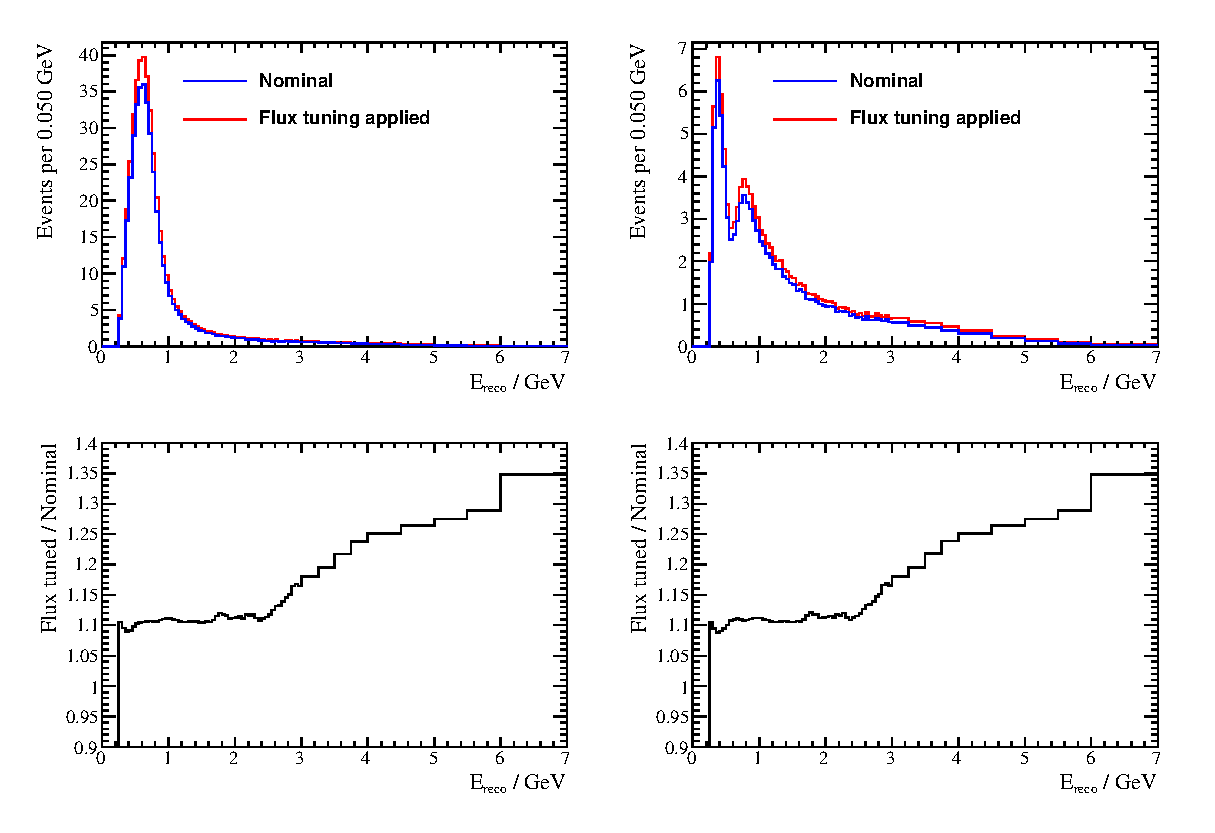
\includegraphics[width=30pc]{./images/spectrum_predictions/spectra_nom_fluxtuned}
\caption {
Top: Reconstructed-energy spectrum of 1 $\mu$-like ring events,
for an exposure of 6.5700$\times$10$^{20}$ POT,
both with and without the effect of the NA61 flux tuning of the nominal MC templates.
The spectra are shown both for no oscillations (left)
and for oscillations with $\sin^{2}\theta_{23}$=0.5, $|\Delta m^{2}_{32}|$=2.4$\times$10$^{-3}$ eV$^{2}$/c$^{4}$,
the 2012 PDG values for $\sin^{2}\theta_{13}$, $\sin^{2}\theta_{12}$ and $\Delta m^{2}_{21}$, and
$\delta_{CP}$=0 (right). Results shown for the normal hierarchy.
Bottom: Ratio of flux-tuned spectrum to the nominal MC spectrum.
}
\label{fig:1Rmu_spectrum_w_and_wo_na61_weights}
\end{figure*}

\begin{figure*}[htb]
\center
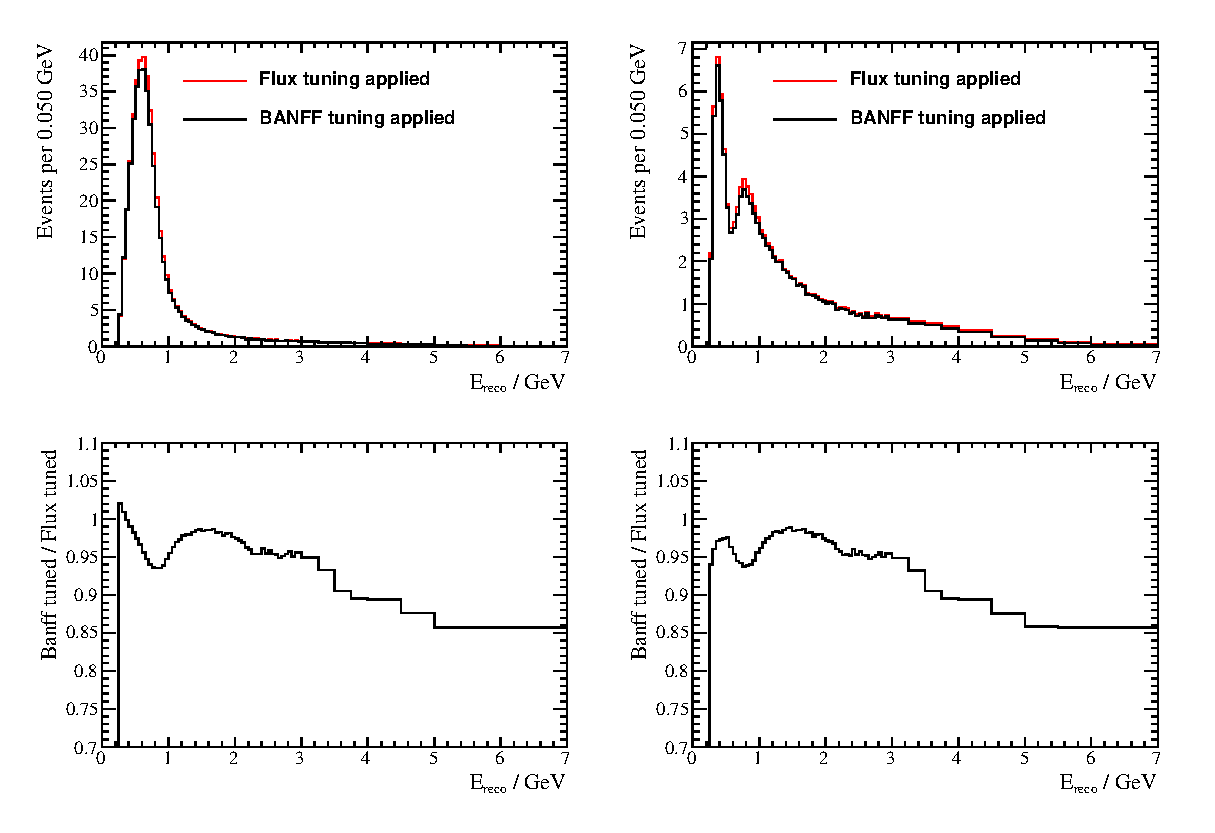
\includegraphics[width=30pc]{./images/spectrum_predictions/spectra_tun_banfftuned}
\caption {
Top: Reconstructed-energy spectrum of 1 $\mu$-like ring events,
for an exposure of 6.5700$\times$10$^{20}$ POT,
both with and without the effect of BANFF flux and cross-section tuning on the NA61-tuned flux MC templates.
The spectra are shown both for no 23-sector oscillations (left)
and for oscillations with $\sin^{2}\theta_{23}$=0.5 and $|\Delta m^{2}_{32}|$=2.4$\times$10$^{-3}$ eV$^{2}$/c$^{4}$ (right).
In all spectra, the 2012 PDG parameters are used for $\sin^{2}\theta_{13}$, $\sin^{2}\theta_{12}$ and $\Delta m^{2}_{21}$
and $\delta_{CP}$=0. Results shown for the normal hierarchy.
Bottom: Ratio of BANFF-tuned spectrum to the flux-tuned spectrum.
}
\label{fig:1Rmu_spectrum_w_and_wo_banff_weights}
\end{figure*}


\clearpage

\section {Systematic effects in the prediction of the single $\mu$-like ring event energy spectrum}
\label{sec:systematics}

%....................................................................................................................
%....................................................................................................................

\subsection {Input systematic parameters}
\label{sec:systematics:inputs}

This analysis considers 45 systematic parameters which can be grouped into 5 categories:

\begin{enumerate}

\item 
{\bf SuperK energy scale} (1 parameter).\\
The systematic parameter $f_{E; r}^{SK}$ is included to control the energy scale.
Its uncertainty is estimated to be 2.4\% \cite{SuperkEScale2013}.
The effect of the uncertainty in the reconstructed energy scale is calculated by scaling the bin edges of
the MC templates and, assuming uniform distribution of events within the bins, calculating the number
of events gained from / lost to neighbouring bins. 
The effect of the energy scale uncertainty is propagated to all MC templates as shown in Tab.\ \ref{tab:apply_syst_to_templates}.\\

\item 
{\bf SuperK efficiencies \& effects of intranuclear and secondary re-interactions} (6 parameters).\\
There are uncertainties in the efficiencies of the fiducial volume and reduction chain, 
and the OD, ring-counting, PID, momentum and decay-electron cuts.
These uncertainties have been evaluated by comparing 1412 days of SK-IV atmospheric data
with atmospheric neutrino Monte Carlo.
Ring counting errors are evaluated using $\nu_\mu$ CCQE, $\nu_\mu$ CCnQE, NC, and $\nu_e$ CC-enriched control samples.
The NC PID error is evaluated using a NC-enriched control sample, which
does not use PID information.
Each Monte Carlo control sample is fitted to the data using the efficiency as a fit parameter, and the uncertainties in the 
efficiencies are estimated by adding the covariance matrix containing the differences between the best-fit and nominal efficiencies to 
the covariance matrix containing the statistical errors in the fitted efficiencies \cite{SuperkErrors2013}.

Intranuclear final-state interactions (FSI) have significant effects in the T2K energy range and
result in event topologies, for scattering from nuclear targets, which are drastically different from 
those created in neutrino scattering from free nucleons.
Uncertainties due to FSI were estimated by simultaneously varying the NEUT parameters that scale the interaction probabilities for quasi-elastic 
scattering, absorption, charge exchange and pion production using the method described in Sec.\ 2 in \cite{NIWGErr}. The NIWG group produced 16 
parameter sets that span the 1$\sigma$ surface in the parameter space; this was done by varying the NEUT parameters when running the pion scattering 
simulations, and comparing the results with external pion-carbon scattering data. These 16 parameter sets are shown in Tab.\ 2 in \cite{NIWGErr}. 
Uncertainties due to secondary pion interactions (SI) were also evaluated. The NIWG group adapted the NEUT nuclear cascade model to simulate SI in the 
SuperK detector simulation (SKDETSIM) and to allow variations in the interaction probabilities. Details of this are given in \cite{SI}. 
Since the same model is used for FSI and SI, it is possible to evaluate the uncertainties in both FSI and SI simultaneously. This was done by 
reweighting a single $\mu$-like ring selected SK MC with the 16 FSI parameter sets using T2KReweight. The reweighting method for FSI is described 
in Sec. 8 in \cite{NEUTnuclear}. Variations in the SI interaction probabilities were included for each FSI parameter set.  Subsequently a covariance 
matrix was calculated using equation 1 in \cite{NIWGErr}; the quantity p in that equation is the average event weight for a FSI parameter set, and 
the sum is over the parameter sets.

In this analysis, we consider the SuperK detector efficiency and FSI/SI systematics together, and add their covariance matrices linearly. Each of 
these covariance matrices has six correlated parameters, corresponding to different modes and reconstructed energy bins, as shown in Tab.\ \ref{tab:input_uncertainties}.
These efficiency/FSI/SI systematics are applied to the MC templates as shown in Tab.\ \ref{tab:apply_syst_to_templates}.\\

\item 
{\bf Correlated flux and cross-section (BANFF) parameters} (23 parameters).\\
The postfit uncertainties of all BANFF flux and cross-section parameters and their correlations are taken into account.
For the disappearance analysis, we use a version of the BANFF fit which considers
only the $\nu_\mu$ and $\bar{\nu}_{\mu}$ flux parameters. The effect of the $\nu_{e}$ and $\bar{\nu}_{e}$ 
flux parameter uncertainties was studied and it was found to be negligible \cite{OurRun123DisappAnalysis3Flavour}.
Only those cross-section parameters that are expected to have some cancellation between the ND280 and SuperK are included in the BANFF fit.
%The other cross-section parameters included in this analysis are taken to be uncorrelated with the flux parameters
%and to have no cancellation between the near and far detectors. These uncorrelated cross-section parameters are discussed below.
A list of the BANFF parameters, their best-fit values and their prefit and postfit errors is given in Tab.\ \ref{tab:input_uncertainties}.

The BANFF parameters are applied to the MC templates as specified in Tab.\ \ref{tab:apply_syst_to_templates}.
All but two of the BANFF cross-section parameters are simple normalization factors.
The parameters $f_{16; t, r}^{banff}$ and $f_{17; t, r}^{banff}$ are
the axial masses that are parameters in the models of neutrino CC quasi-elastic ($M_{A}^{QE}$) 
and resonance-production ($M_{A}^{RES}$) interactions respectively;
these have a more complicated, often non-linear, dependence on true and reconstructed neutrino energy.
Event reweighting methods were used to obtain the fractional changes of the number of events, 
in bins of true and reconstructed neutrino energy, for a range of values (-3.0$\sigma$, -2.5$\sigma$, -2.0$\sigma$, ..., +3.0$\sigma$)
in the $f_{16; t, r}^{banff}$ and $f_{17; t, r}^{banff}$ parameters.
In our p.d.f. calculation, cubic splines\footnote{
  In this analysis, the cubic splines are computed for each non-linear systematic and for each MC template,
  in bins of reconstructed and true energy. To produce these splines, we use the SK13a SuperK MC, the 11bv3.2 flux weights and 
  the following oscillation parameters: $\sin^{2}(2\theta_{23})$ = 1.0, $\sin^{2}(2\theta_{13})$ = 0.098, $\sin^{2}(2\theta_{12})$ = 
  0.8495, $|\Delta m^{2}_{32}|$ = 2.44$\times$10$^{-3}$ eV$^{2}$/c$^{4}$, $\Delta m^{2}_{21}$ = 7.5$\times$10$^{-5}$ eV$^{2}$/c$^{4}$, 
  $\delta_{CP}$ = 0 and the normal mass hierarchy. For all splines, we use 41 bins in reconstructed energy:
  1 bin from 0-0.3 GeV, 14 50-MeV bins from 0.3-1.0 GeV, 20 100-MeV bins from 1.0-3.0 GeV, 2 500-MeV bins from 3.0-4.0 GeV
  1 bin from 4.0-5.0 GeV, 1 bin from 5.0-7.0 GeV, 1 bin from 7.0-10.0 GeV and 1 bin from 10.0-30.0 GeV.
  The $\nu_{\mu}$, $\bar{\nu}_{\mu}$ and oscillated $\nu_{e}$ samples have 11 bins in true energy:
  1 bin from 0-0.4 GeV, 3 100-MeV bins from 0.4-0.7 GeV, 1 bin from 0.7-1.0 GeV, 1 bin from 1.0-1.5 GeV, 2 1-GeV bins from 1.5-3.5 GeV,
  1 bin from 3.5-5.0 GeV, 1 bin from 5.0-7.0 GeV and 1 bin from 7.0-30.0 GeV.
  The $\nu_{e}$ and oscillated $\nu_\mu$ samples have 7 bins in true energy:
  1 bin from 0-0.05 GeV, 1 bin from 0.5-0.7 GeV, 1 bin from 0.7-0.8 GeV,
  1 bin from 0.8-1.5 GeV, 1 bin from 1.5-2.5 GeV, 1 bin from 2.5-4.0 GeV and 1 bin from 4.0-30.0 GeV.
  Finally, the $\bar{\nu}_{e}$ sample have 2 bins in true energy:
  1 bin from 0-2.5 GeV and 1 bin from 2.5-30.0 GeV.\\
  The binning of the cubic splines was studied, and the results were presented in Appendix I of \cite{OurRun123DisappAnalysis3Flavour}.
  The spline spectra produced using the cubic splines are very similar to those produced using the CPU-intensive event-by-event reweighting,
  especially for the dominant components of the spectra. 
} 
are used to interpolate between these event weights 
to obtain the fractional change for any value of these systematic parameters in the (-3.0$\sigma$, +3.0$\sigma$) range.\\

\item 
{\bf Uncorrelated cross-section parameters}(11 parameters).\\
In addition to the BANFF cross-section systematics,
another 11 cross-section systematics are taken into account; these additional systematics are considered to be uncorrelated 
between themselves and to have no cancellation between the near and far detectors \cite{NIWGErr} \cite{MoreNIWGErr113} \cite{NIWGNuBarErr}.

Three of these additional systematics relate to the initial-state nuclear environment modelling for CCQE.
Neutrino Monte Carlo generators typically use Relativistic Fermi Gas (RFG) models,
with or without extensions to take nucleon-nucleon correlation into account, 
and with some, often simplistic, prescription for the treatment of off-shell kinematics.
The RFG model implementation depends on two parameters, the Fermi momentum level (225 MeV for $^{16}O$)
and the nucleon binding energy (27 MeV for $^{16}O$), which are extracted from quasi-elastic electron scattering data.
The systematic parameter $f_{pF; t, r}$ takes into account the effect of a 30 MeV 1$\sigma$ uncertainty in the Fermi momentum level
for $^{16}O$, while the parameter $f_{bindE; t, r}$ takes into account the effect of a 9 MeV 1$\sigma$ uncertainty in the nucleon 
binding energy for for $^{16}O$.
The implementation details of the nuclear model can have a significant effect and, therefore,
the effect of switching between two such models was also included as a systematic uncertainty.
This analysis considers the effect of switching between the RFG model and a better-motivated 
Spectral Function (SF) model. The latter does not assume a fixed binding energy and includes the 
correlations between nucleon momentum and binding energy. The systematic parameter $f_{SF; t, r}$ 
includes the effect of switching between the two models.

Simple, energy-independent, generator-level uncertainties are considered for the CC coherent, NC, $\nu_e$ CC
and $\bar{\nu}$ CC cross sections, as the effect of these processes in the single $\mu$-like ring sample is small.
This analysis uses a 100\% uncertainty for the CC coherent cross-section, 
a 30\% uncertainty for both the NC1$\pi^\pm$ and NC ``other'' (all but single $\pi^\pm$) cross section,
a 3\% uncertainty on the $\nu_e$ / $\nu_\mu$ CC cross-section ratio and 
a 20\% uncertainty on the $\bar{\nu}$ / $\nu$ CC cross-section ratio.
The effect of the variation of the above cross sections is included in the analysis
through the systematic parameters $f_{CCcoh; t}$, $f_{NC1\pi^\pm; t}$, $f_{NCoth; t}$,
$f_{CC\nu_e; t}$ and $f_{CC\bar{\nu}; t}$ respectively.

The treatment of $\Delta$ resonances in the nuclear environment has been controversial in the neutrino
Monte Carlo generator community. Certain models include a ~20\%-level of $\pi$-less $\Delta$ decays in order
to include the effect of $\Delta+N \rightarrow N+N$ scattering, in which the $\Delta$ interacts before it can decay. 
In contrast, other models include no $\pi$-less 
$\Delta$ decays on the basis that this would amount to double counting since, whatever the size of the effect, 
it is already included in hadron-nucleus scattering data to which the intranuclear cascade Monte Carlos are tuned.
This analysis uses NEUT, in which 20\% of $\Delta$s have a $\pi$-less decay by default, and takes the uncertainty in this 
branching fraction to be 100\%. 
The systematic parameter $f_{\pi-less\Delta; t, r}$ includes the effect of varying the fraction of $\pi$-less $\Delta$ 
decays to the corresponding MC templates.

The $f_{CCothShape;t,r}$ systematic parameterizes the uncertainty in CC multi-pion, CC deep inelastic scattering and CC $\eta$, 
K and photon production. From MINOS data, this is known to be $\approx$10\% at 4 GeV. Using this as a reference point, 
the uncertainty is estimated as 0.4/E$_{\nu}$, where E$_{\nu}$ is in GeV. It might appear that this error could diverge at 
low energy, but this does not happen since the threshold is $\approx$0.6 GeV and there are very 
few interactions below 1 GeV. 

The $f_{Wshape;t,r}$ parameter modifies the shape of the initial pion momentum distribution (before final-state interactions) 
by changing the distribution of the pion/nucleon invariant mass while keeping the total cross section constant. As the 
W shape parameter decreases, the pion momentum shifts to lower values, and this increases the probability of pion 
absorption in a final-state interaction. If such an absorption occurs, the event is migrated from CC1$\pi$ (its 
true initial state) and appears to be CCQE.

The effect of the $f_{CCcoh; t}$, $f_{NC1\pi^\pm; t}$, $f_{NCoth; t}$, $f_{CC\nu_e; t}$ and $f_{CC\bar{\nu}; t}$ 
systematic parameters is a simple normalisation change for the corresponding MC templates and thus easily implemented.
Systematic parameters $f_{pF; t, r}$, $f_{SF; t, r}$, $f_{bindE; t, r}$, $f_{\pi-less\Delta; t, r}$, $f_{CCothShape; t, r}$ 
and $f_{Wshape; t, r}$  have a complicated, often non-linear, dependence on true and reconstructed energy.
These are treated in a similar way to the BANFF parameters $f_{16; t, r}^{banff}$ and $f_{17; t, r}^{banff}$.
Event reweighting methods were used to obtain the fractional changes of the number of events, 
in bins of true and reconstructed neutrino energy, for a range of values (-3.0$\sigma$, -2.5$\sigma$, -2.0$\sigma$, ..., +3.0$\sigma$)
of the systematic parameters. Again cross-section splines with polynomials of order 3 were used to interpolate between these event 
weights to obtain the fractional change for any
value of these systematic parameters in the (-3.0$\sigma$, +3.0$\sigma$) range.

Some of these systematics are special cases:
{
\begin{itemize}
\item 
  $f_{SF; t, r}$ is discrete; it can be either spectral function off (RFG) or spectral function on (SF). 
  Splines are generated with SF off as nominal (0), and SF on as +1$\sigma$.
  This parameter is restricted to the range between 0 and +1$\sigma$, and linear interpolation is made between the weights 
  for nominal and +1$\sigma$.
\item 
  For $f_{Wshape; t, r}$ only $\pm$1$\sigma$ errors are evaluated using event reweighting. 
  Weights for positive tweaks are interpolated or extrapolated from the nominal and +1$\sigma$ weights, and weights for negative 
  tweaks are interpolated or extrapolated from the nominal and -1$\sigma$ weights.
\item 
  For $f_{\pi-less\Delta; t, r}$ only $\pm$1.0 sigma errors are evaluated using event reweighting.
  Weights for positive tweaks are interpolated or extrapolated from the nominal and +1$\sigma$ weights, and weights for tweaks between 
  nominal and -1$\sigma$ are interpolated from the nominal and -1$\sigma$ weights. Weights for tweaks more negative than 
  -1$\sigma$ are taken to be the same as the -1$\sigma$ weight; this is done since 20\% of $\Delta$s have a $\pi$-less decay by 
  default in NEUT, and the error is 20\%. For this reason, it is unphysical to tweak $f_{\pi-less\Delta; t, r}$ to be 
  more negative than -1$\sigma$. 
\end{itemize}
}

The 11 uncorrelated cross-section systematics considered in this analysis are summarised in Tab.\ \ref{tab:input_uncertainties}.
These cross-section systematics are applied to the MC templates as shown in Tab.\ \ref{tab:apply_syst_to_templates}.\\

\item {\bf \emph{Non-23 sector} oscillation parameters} (4 parameters).\\
In this analysis, we treat all four non-23-sector oscillation parameters as nuisance parameters in the fit. We use penalty terms 
for $\sin^2\theta_{13}$, $\sin^2\theta_{12}$ and $\Delta m^2_{21}$, with their central values and uncertainties being taken from 
\cite{PDG2012,FogliLisi}. The CP-violating phase $\delta_{CP}$ can take any value between $-\pi$ and $+\pi$, and is not 
constrained by a penalty term. 
\end{enumerate}

% Multi-nucleon effects are not taken into account in the fit.
% Estimates of the size of the effect are given in Appendix \ref{appendix:mec}.

\clearpage

% ................................................................................................................

%
% Table summarizing systematics
%

{
\small
\renewcommand{\arraystretch}{2.0} % enlarge line spacing
\begin{longtable}{p{1.65cm}l}
%
% SuperK & FSI+SI
%
\hline
\multicolumn {2}{l} { {\bf SuperK energy scale systematics (1)} } \\
\hline
  \parbox{0.15\textwidth}
  {
    $f_{E; r}^{SK}$ 
  }
& 
  \parbox{0.81\textwidth}
  {
    \vspace{0.2cm}
    Reconstructed energy scale systematic.
    The uncertainty is estimated to be 2.4\% \cite{SuperkEScale2013}.
    \vspace{0.2cm}
  }
\\
\hline
\multicolumn {2}{l} { {\bf SuperK detector efficiency \& intranuclear and
    secondary interaction systematics} } \\
\hline
  \parbox{0.15\textwidth}
  {
     $f_{i; r}^{SK+FSI}$
  }
&
  \parbox{0.81\textwidth}
  {
    \vspace{0.2cm}
    SuperK detector efficiency (ring counting, fiducial volume, reduction chain, OD cut, PID cut, momentum cut and 
    decay electron cut efficiency uncertainties), 
    FSI (final state interaction / intranuclear hadron transport) and
    SI (secondary interaction / detector hadron transport) systematic parameters.
    Six correlated parameters are included (i=0,...,5) corresponding to different modes and reconstructed energy bins.\\
    $$     
        {
         \renewcommand{\arraystretch}{1.0} % enlarge line spacing
         \begin{array}{c|c|c}
            \text{Parameter} & \text{Description} & 1\sigma \text{ fractional error} \\
            0 &  \nu_\mu \text{ \& } \bar{\nu}_{\mu} \text{ CCQE, } E_{reco} < \text{ 0.4 GeV}                              & 0.025   \\
            1 &  \nu_\mu \text{ \& } \bar{\nu}_{\mu} \text{ CCQE, } \text{0.4 GeV} \leq E_{reco} \leq \text{ 1.1 GeV}       & 0.028   \\
            2 &  \nu_\mu \text{ \& } \bar{\nu}_{\mu} \text{ CCQE, } E_{reco} > \text{ 1.1 GeV}                              & 0.037   \\
            3 &  \nu_\mu \text{ \& } \bar{\nu}_{\mu} \text{ CCnonQE}                                                        & 0.119   \\
            4 &  \nu_e \text{ \& } \bar{\nu}_{e} \text{ CC}                                                                 & 1.000   \\
            5 &  \text{All NC}                                                                                              & 0.600   \\
         \end{array} }
    $$\\
    The covariance matrix is listed in Eq.\ \ref{eq:Cskfsi}.\\
    \vspace{0.2cm}
  }
\\
%
% BANFF systematics
%
\hline
\multicolumn {2}{l} { {\bf Correlated flux and cross-section (BANFF) systematics} (23)} \\
\hline
  \parbox{0.15\textwidth}
  {
     $f_{i; t, r}^{banff}$
  }
&
  \parbox{0.81\textwidth}
  {
    \vspace{0.2cm}
    Flux and cross-section parameters tuned by BANFF group on ND280 data \cite{BANFF2013}. 
    Twenty-three correlated parameters are included (i=0,...,22).\\
    $$     
        {
         \renewcommand{\arraystretch}{1.0} % enlarge line spacing
         \begin{array}{c|c|c|c}
           \text{Parameter} & \text{Description} & \text{Best-fit} & 1\sigma \text{ pre/postfit} \\
           & & & \text{fractional error} \\
            0 &  \nu_\mu \text{ flux normalisation, E = 0.0 - 0.4 GeV}          & 1.029 & 0.121 / 0.085 \\
            1 &  \nu_\mu \text{ flux normalisation, E = 0.4 - 0.5 GeV}          & 1.022 & 0.130 / 0.088 \\
            2 &  \nu_\mu \text{ flux normalisation, E = 0.5 - 0.6 GeV}          & 0.995 & 0.122 / 0.080 \\
            3 &  \nu_\mu \text{ flux normalisation, E = 0.6 - 0.7 GeV}          & 0.966 & 0.115 / 0.076 \\
            4 &  \nu_\mu \text{ flux normalisation, E = 0.7 - 1.0 GeV}          & 0.934 & 0.129 / 0.085 \\
            5 &  \nu_\mu \text{ flux normalisation, E = 1.0 - 1.5 GeV}          & 0.992 & 0.116 / 0.077 \\
            6 &  \nu_\mu \text{ flux normalisation, E = 1.5 - 2.5 GeV}          & 1.037 & 0.100 / 0.068 \\
            7 &  \nu_\mu \text{ flux normalisation, E = 2.5 - 3.5 GeV}          & 1.054 & 0.095 / 0.065 \\
            8 &  \nu_\mu \text{ flux normalisation, E = 3.5 - 5.0 GeV}          & 1.035 & 0.112 / 0.072 \\
            9 &  \nu_\mu \text{ flux normalisation, E = 5.0 - 7.0 GeV}          & 0.975 & 0.152 / 0.073 \\
           10 &  \nu_\mu \text{ flux normalisation, E = 7.0 - 30.0 GeV}         & 0.943 & 0.187 / 0.082 \\
           11 &  \bar{\nu}_{\mu} \text{ flux normalisation, E = 0.0 - 0.7 GeV}  & 1.030 & 0.133 / 0.102 \\
           12 &  \bar{\nu}_{\mu} \text{ flux normalisation, E = 0.7 - 1.0 GeV}  & 1.011 & 0.117 / 0.090 \\
           13 &  \bar{\nu}_{\mu} \text{ flux normalisation, E = 1.0 - 1.5 GeV}  & 1.007 & 0.119 / 0.094 \\
           14 &  \bar{\nu}_{\mu} \text{ flux normalisation, E = 1.5 - 2.5 GeV}  & 1.026 & 0.123 / 0.104 \\
           15 &  \bar{\nu}_{\mu} \text{ flux normalisation, E = 2.5 -30.0 GeV}  & 1.008 & 0.122 / 0.107 \\
           16 &  \text{CCQE axial-mass scaling factor}                          & 1.025 & 0.372 / 0.059 \\
           17 &  \text{Resonance-production axial-mass scaling factor}          & 0.797 & 0.183 / 0.056 \\
           18 &  \text{CCQE normalisation, E = 0.0 - 1.5 GeV}                   & 0.966 & 0.110 / 0.076 \\
           19 &  \text{CCQE normalisation, E = 1.5 - 3.5 GeV}                   & 0.931 & 0.300 / 0.103 \\
           20 &  \text{CCQE normalisation, E = 3.5 - 30.0 GeV}                  & 0.852 & 0.300 / 0.114 \\
           21 &  CC1\pi \text{ normalisation, E = 0.0 - 2.5 GeV}                & 1.265 & 0.317 / 0.163 \\
           22 &  CC1\pi \text{ normalisation, E = 2.5 - 30.0 GeV}               & 1.122 & 0.400 / 0.172 \\
         \end{array} }
    $$\\
    The covariance matrix is listed in Eq.\ \ref{eq:Cbanff}.\\
    \vspace{0.2cm}
  }
  \\
\vspace{1cm}\\
%
% Uncorrelated cross-section
%
\hline
\multicolumn {2}{l} { {\bf Uncorrelated cross-section systematics} (11)} \\
\hline
  \parbox{0.15\textwidth}
  {
    \vspace{0.1cm}
    $f_{pF; t, r}$
    \vspace{0.1cm}
  }
&
  \parbox{0.81\textwidth}
  {
    \vspace{0.1cm}
    Uncertainty in Fermi momentum for $^{16}O$ was taken to be 225$\pm$30 MeV \cite{MoreNIWGErr113}.
    \vspace{0.1cm}
  }
\\
  \parbox{0.15\textwidth}
  {
    \vspace{0.1cm}
    $f_{bindE; t, r}$
    \vspace{0.1cm}
  }
&
  \parbox{0.81\textwidth}
  {
    \vspace{0.1cm}
    Uncertainty in binding energy for $^{16}O$ was taken to be 27$\pm$9 MeV \cite{MoreNIWGErr113}.
    \vspace{0.1cm}
  }
\\
  \parbox{0.15\textwidth}
  {
    \vspace{0.1cm}
    $f_{SF; t, r}$
    \vspace{0.1cm}
  }
&
  \parbox{0.81\textwidth}
  {
    \vspace{0.1cm}
    Nuclear environment modelling systematic:
    Switches from Fermi Gas (RFG) to Spectral Function (SF) model (0:RFG - 1:SF) \cite{MoreNIWGErr113}.
    \vspace{0.1cm}
  }
\\
  \parbox{0.15\textwidth}
  {
    \vspace{0.1cm}
    $f_{\pi-less\Delta; t, r}$
    \vspace{0.1cm}
  }
&
  \parbox{0.81\textwidth}
  {
    \vspace{0.1cm}
    Systematic due to the uncertainty (20\% \cite{MoreNIWGErr113}).
    in the fraction of $\pi$-less $\Delta$ decays in resonance-production events.
    \vspace{0.1cm}
  }
\\
  \parbox{0.15\textwidth}
  {
    \vspace{0.1cm}
    $f_{CCothShape; t, r}$
    \vspace{0.1cm}
  }
&
  \parbox{0.81\textwidth}
  {
    \vspace{0.1cm}
    Systematic due to the uncertainty (40\% \cite{MoreNIWGErr113}) in CC multipion, CC DIS and CC resonant $\eta$, K and photon production cross section.
    \vspace{0.1cm}
  }
\\
  \parbox{0.15\textwidth}
  {
    \vspace{0.1cm}
    $f_{Wshape; t, r}$
    \vspace{0.1cm}
  }
&
  \parbox{0.81\textwidth}
  {
    \vspace{0.1cm}
    Systematic due to the uncertainty (52\% \cite{MoreNIWGErr113}) in the shape of the 
    initial pion momentum distribution (before final-state interactions) in resonance interactions. 
    \vspace{0.1cm}
  }
\\
  \parbox{0.15\textwidth}
  {
    \vspace{0.1cm}
    $f_{CCcoh; t}$
    \vspace{0.1cm}
  }
&
  \parbox{0.81\textwidth}
  {
    \vspace{0.1cm}
    Systematic due to the uncertainty (100\% \cite{MoreNIWGErr113}) in the CC coherent cross section.
    \vspace{0.1cm}
  }
\\
  \parbox{0.15\textwidth}
  {
    \vspace{0.1cm}
    $f_{NC1\pi^\pm; t}$
    \vspace{0.1cm}
  }
&
  \parbox{0.81\textwidth}
  {
    \vspace{0.1cm}
    Systematic due to the uncertainty (30\% \cite{MoreNIWGErr113}) on the NC1$\pi^\pm$ cross section.
    \vspace{0.1cm}
  }
\\
  \parbox{0.15\textwidth}
  {
    \vspace{0.1cm}
    $f_{NCoth; t}$
    \vspace{0.1cm}
  }
&
  \parbox{0.81\textwidth}
  {
    \vspace{0.1cm}
    Systematic due to the uncertainty (30\% \cite{MoreNIWGErr113}) on the NC other (all but single $\pi^\pm$) cross section.
    \vspace{0.1cm}
  }
\\
  \parbox{0.15\textwidth}
  {
    \vspace{0.1cm}
    $f_{CC\nu_e; t}$
    \vspace{0.1cm}
  }
&
  \parbox{0.81\textwidth}
  {
    \vspace{0.1cm}
    Systematic due to the uncertainty (3\% \cite{NIWGErr}) on the $\nu_e$ / $\nu_\mu$ CC cross-section ratio.
    \vspace{0.1cm}
  }
\\
  \parbox{0.15\textwidth}
  {
    \vspace{0.1cm}
    $f_{CC\bar{\nu}; t}$
    \vspace{0.1cm}
  }
&
  \parbox{0.81\textwidth}
  {
    \vspace{0.1cm}
    Systematic due to the uncertainty (20\% \cite{NIWGNuBarErr}) on the $\bar{\nu}$ / $\nu$ CC cross-section ratio.
    \vspace{0.1cm}
  }
\\
  %
  % Oscillation parameter
  % 
  \hline
  \multicolumn {2}{l} { {\bf \emph{Non-23 sector} oscillation parameters} (4)} \\
  \hline
  \parbox{0.15\textwidth}
  {
    \vspace{0.1cm}
    $\sin^2\theta_{13}$
  }
&
  \parbox{0.81\textwidth}
  {
    \vspace{0.1cm}
    Uncertainty in $\sin^2\theta_{13}$ of 13.9\%, taken from the 2012 PDG \cite{PDG2012}.
    \vspace{0.1cm}
  }
\\
  \parbox{0.15\textwidth}
  {
    \vspace{0.1cm}
    $\sin^2\theta_{12}$
  }
&
  \parbox{0.81\textwidth}
  {
    \vspace{0.1cm}
    Uncertainty in $\sin^2\theta_{12}$ of 5.9\%, taken from a global fit \cite{FogliLisi}.
    \vspace{0.1cm}
  }
\\
  \parbox{0.15\textwidth}
  {
    \vspace{0.1cm}
    $\Delta m^2_{21}$
  }
&
  \parbox{0.81\textwidth}
  {
    \vspace{0.1cm}
    Uncertainty in  $\Delta m^2_{21}$ of 2.7\%, taken from the 2012 PDG \cite{PDG2012}.
    \vspace{0.1cm}
  }
\\
  \parbox{0.15\textwidth}
  {
    \vspace{0.1cm}
    $\delta_{CP}$
  }
&
  \parbox{0.81\textwidth}
  {
    \vspace{0.1cm}
    Allowed to vary between -$\pi$ and +$\pi$ with no constraint.
    \vspace{0.1cm}
  }\\
\caption{
   Summary of systematics included the {\em VALOR} Run 1+2+3+4 $\nu_{\mu}$-disappearance analysis.
   %The nuisance parameter symbols used in this paper are shown in the first column.
   %An index r in the nuisance parameter symbol denotes dependence on reconstructed energy while an index t denotes
   %dependence on true energy.
   %An index i is used where multiple systematic parameters, typically correlated between themselves, are grouped together.
}\\
\label{tab:input_uncertainties}\\
\end{longtable}
}

% 
% ................................................................................................................
% 

%
% Equation with SK+FSI covariance matrix
%
%make with test_analysis_inputs.C
{
\tiny
\begin{sideways}
\begin{minipage}{23cm}
{
\setlength{\arraycolsep}{1pt}
\begin{equation}
C^{SK+FSI} = \end{equation}
\begin{equation*}
\begin{blockarray}{c p{20pt}p{20pt}p{20pt}p{20pt}p{20pt}p{20pt}p{20pt}p{20pt}p{20pt}p{20pt}p{20pt}p{20pt}p{20pt}p{20pt}p{20pt}p{20pt}p{20pt}p{20pt}}
                  &     \begin{sideways}  {\color{blue} $f_{0; r}^{SK+FSI}$}  \end{sideways} &    \begin{sideways}   {\color{blue} $f_{1; r}^{SK+FSI}$}  \end{sideways} &     \begin{sideways}  {\color{blue} $f_{2; r}^{SK+FSI}$}  \end{sideways} &  \begin{sideways}     {\color{blue} $f_{3; r}^{SK+FSI}$} \end{sideways} &      \begin{sideways} {\color{blue} $f_{4; r}^{SK+FSI}$} \end{sideways} &    \begin{sideways}   {\color{blue} $f_{5; r}^{SK+FSI}$} \end{sideways} &    \begin{sideways}   {\color{blue}  $f_{6; r}^{SK+FSI}$}\end{sideways} &   \begin{sideways}    {\color{blue} $f_{7; r}^{SK+FSI}$}  \end{sideways} &   \begin{sideways}    {\color{blue} $f_{8; r}^{SK+FSI}$} \end{sideways} &   \begin{sideways}    {\color{blue} $f_{9; r}^{SK+FSI}$} \end{sideways} &   \begin{sideways}    {\color{blue} $f_{10; r}^{SK+FSI}$} \end{sideways} &   \begin{sideways}    {\color{blue} $f_{11; r}^{SK+FSI}$} \end{sideways} &    \begin{sideways}   {\color{blue} $f_{12; r}^{SK+FSI}$} \end{sideways} &    \begin{sideways}   {\color{blue} $f_{13; r}^{SK+FSI}$} \end{sideways} &   \begin{sideways}    {\color{blue}$ f_{14; r}^{SK+FSI}$}\end{sideways} &   \begin{sideways}    {\color{blue} $f_{15; r}^{SK+FSI}$}  \end{sideways} &    \begin{sideways}   {\color{blue} $f_{16; r}^{SK+FSI}$} \end{sideways} &   \begin{sideways}    {\color{blue} $f_{17; r}^{SK+FSI}$} \end{sideways}\\ 
\begin{block}{c(p{20pt}p{20pt}p{20pt}p{20pt}p{20pt}p{20pt}p{20pt}p{20pt}p{20pt}p{20pt}p{20pt}p{20pt}p{20pt}p{20pt}p{20pt}p{20pt}p{20pt}p{20pt}@{\hspace*{1pt}})}
      {\color{blue} f_{0; r}^{SK+FSI}}  \vspace{0.2cm} &        {\color{red} 0.00040} &              0.00037 &              0.00031 &              0.00028 &              0.00039 &              0.00022 &              0.00021 &              0.00032 &              0.00006 &              0.00020 &              0.00019 &              0.00020 &              0.00020 &              0.00027 &             -0.00017 &              0.00019 &              0.00018 &              0.00018 \\ 
      {\color{blue} f_{1; r}^{SK+FSI}}  \vspace{0.2cm} &              0.00037 &        {\color{red} 0.00037} &              0.00033 &              0.00037 &              0.00383 &              0.00026 &              0.00029 &              0.00030 &              0.00010 &              0.00015 &              0.00015 &              0.00014 &              0.00026 &              0.00028 &             -0.00007 &              0.00020 &              0.00019 &              0.00024 \\ 
      {\color{blue} f_{2; r}^{SK+FSI}}  \vspace{0.2cm} &              0.00031 &              0.00033 &        {\color{red} 0.00040} &              0.00079 &              0.00408 &              0.00030 &              0.00055 &              0.00027 &              0.00022 &              0.00027 &              0.00022 &              0.00017 &              0.00041 &              0.00033 &              0.00026 &              0.00019 &              0.00020 &              0.00032 \\ 
      {\color{blue} f_{3; r}^{SK+FSI}}  \vspace{0.2cm} &              0.00028 &              0.00037 &              0.00079 &        {\color{red} 0.00871} &              0.00345 &              0.00226 &              0.00927 &              0.00124 &              0.00075 &              0.00299 &              0.00122 &              0.00036 &              0.00558 &              0.00308 &              0.00296 &             -0.00113 &             -0.00123 &              0.00219 \\ 
      {\color{blue} f_{4; r}^{SK+FSI}}  \vspace{0.2cm} &              0.00039 &              0.00383 &              0.00408 &              0.00345 &        {\color{red} 1.00961} &              0.00724 &              0.00156 &              0.00035 &             -0.00001 &             -0.00593 &             -0.00552 &             -0.00594 &              0.00099 &              0.00060 &              0.00011 &             -0.00069 &              0.00128 &              0.00669 \\ 
      {\color{blue} f_{5; r}^{SK+FSI}}  \vspace{0.2cm} &              0.00022 &              0.00026 &              0.00030 &              0.00226 &              0.00724 &        {\color{red} 0.35896} &              0.00036 &              0.00012 &              0.00021 &              0.00125 &              0.00511 &              0.00271 &              0.00012 &             -0.00004 &              0.00018 &              0.01622 &              0.00577 &              0.00064 \\ 
      {\color{blue} f_{6; r}^{SK+FSI}}  \vspace{0.2cm} &              0.00021 &              0.00029 &              0.00055 &              0.00927 &              0.00156 &              0.00036 &        {\color{red} 0.01218} &              0.00173 &              0.00106 &              0.00360 &              0.00196 &              0.00033 &              0.00744 &              0.00407 &              0.00388 &             -0.00050 &             -0.00050 &              0.00323 \\ 
      {\color{blue} f_{7; r}^{SK+FSI}}  \vspace{0.2cm} &              0.00032 &              0.00030 &              0.00027 &              0.00124 &              0.00035 &              0.00012 &              0.00173 &        {\color{red} 0.00095} &              0.00057 &              0.00054 &              0.00038 &              0.00019 &              0.00117 &              0.00110 &              0.00050 &              0.00015 &              0.00009 &              0.00051 \\ 
      {\color{blue} f_{8; r}^{SK+FSI}}  \vspace{0.2cm} &              0.00006 &              0.00010 &              0.00022 &              0.00075 &             -0.00001 &              0.00021 &              0.00106 &              0.00057 &        {\color{red} 0.00120} &              0.00028 &              0.00020 &              0.00011 &              0.00079 &              0.00072 &              0.00182 &              0.00026 &              0.00030 &              0.00047 \\ 
      {\color{blue} f_{9; r}^{SK+FSI}}  \vspace{0.2cm} &              0.00020 &              0.00015 &              0.00027 &              0.00299 &             -0.00593 &              0.00125 &              0.00360 &              0.00054 &              0.00028 &        {\color{red} 1.54760} &              1.51082 &              1.52756 &              0.00218 &              0.00119 &              0.00097 &              0.00056 &             -0.00024 &             -0.00273 \\ 
      {\color{blue} f_{10; r}^{SK+FSI}}  \vspace{0.2cm} &              0.00019 &              0.00015 &              0.00022 &              0.00122 &             -0.00552 &              0.00511 &              0.00196 &              0.00038 &              0.00020 &              1.51082 &        {\color{red} 1.47783} &              1.49290 &              0.00119 &              0.00061 &              0.00044 &              0.00161 &              0.00252 &              0.00080 \\ 
      {\color{blue} f_{11; r}^{SK+FSI}}  \vspace{0.2cm} &              0.00020 &              0.00014 &              0.00017 &              0.00036 &             -0.00594 &              0.00271 &              0.00033 &              0.00019 &              0.00011 &              1.52756 &              1.49290 &        {\color{red} 1.50974} &              0.00028 &              0.00016 &              0.00003 &             -0.00060 &              0.00056 &             -0.00240 \\ 
      {\color{blue} f_{12; r}^{SK+FSI}}  \vspace{0.2cm} &              0.00020 &              0.00026 &              0.00041 &              0.00558 &              0.00099 &              0.00012 &              0.00744 &              0.00117 &              0.00079 &              0.00218 &              0.00119 &              0.00028 &        {\color{red} 0.00466} &              0.00259 &              0.00251 &             -0.00035 &             -0.00028 &              0.00188 \\ 
      {\color{blue} f_{13; r}^{SK+FSI}}  \vspace{0.2cm} &              0.00027 &              0.00028 &              0.00033 &              0.00308 &              0.00060 &             -0.00004 &              0.00407 &              0.00110 &              0.00072 &              0.00119 &              0.00061 &              0.00016 &              0.00259 &        {\color{red} 0.00178} &              0.00139 &             -0.00014 &             -0.00017 &              0.00110 \\ 
      {\color{blue} f_{14; r}^{SK+FSI}}  \vspace{0.2cm} &             -0.00017 &             -0.00007 &              0.00026 &              0.00296 &              0.00011 &              0.00018 &              0.00388 &              0.00050 &              0.00182 &              0.00097 &              0.00044 &              0.00003 &              0.00251 &              0.00139 &        {\color{red} 0.00395} &             -0.00005 &              0.00015 &              0.00124 \\ 
      {\color{blue} f_{15; r}^{SK+FSI}}  \vspace{0.2cm} &              0.00019 &              0.00020 &              0.00019 &             -0.00113 &             -0.00069 &              0.01622 &             -0.00050 &              0.00015 &              0.00026 &              0.00056 &              0.00161 &             -0.00060 &             -0.00035 &             -0.00014 &             -0.00005 &        {\color{red} 0.27476} &              0.06449 &              0.05220 \\ 
      {\color{blue} f_{16; r}^{SK+FSI}}  \vspace{0.2cm} &              0.00018 &              0.00019 &              0.00020 &             -0.00123 &              0.00128 &              0.00577 &             -0.00050 &              0.00009 &              0.00030 &             -0.00024 &              0.00252 &              0.00056 &             -0.00028 &             -0.00017 &              0.00015 &              0.06449 &        {\color{red} 0.06079} &              0.09676 \\ 
      {\color{blue} f_{17; r}^{SK+FSI}}  \vspace{0.2cm} &              0.00018 &              0.00024 &              0.00032 &              0.00219 &              0.00669 &              0.00064 &              0.00323 &              0.00051 &              0.00047 &             -0.00273 &              0.00080 &             -0.00240 &              0.00188 &              0.00110 &              0.00124 &              0.05220 &              0.09676 &        {\color{red} 0.36527} \\ 
\end{block}
\label{eq:Cskfsi}
\end{blockarray}
\end{equation*}
}
\end{minipage}
\end{sideways}
\normalsize
}


%
% Large sideways equation with BANFF covariance matrix
%
%make with test_analysis_inputs.C
{
\tiny
\begin{sideways}
\begin{minipage}{23cm}
{
\setlength{\arraycolsep}{1pt}
\begin{equation}
C^{banff} =\end{equation}
\begin{equation*}
\begin{blockarray}{c p{7pt}p{7pt}p{7pt}p{7pt}p{7pt}p{7pt}p{7pt}p{7pt}p{7pt}p{7pt}p{7pt}p{7pt}p{7pt}p{7pt}p{7pt}p{7pt}p{7pt}p{7pt}p{7pt}p{7pt}p{7pt}p{7pt}p{7pt}p{7pt}p{7pt}p{7pt}p{7pt}p{7pt}p{7pt}p{7pt}p{7pt}p{7pt}p{7pt}}
        & \begin{sideways} {\color{blue} $f_{0; t, r}^{banff}$} \end{sideways} & \begin{sideways} {\color{blue} $f_{1; t, r}^{banff}$} \end{sideways} & \begin{sideways} {\color{blue} $f_{2; t, r}^{banff}$} \end{sideways} & \begin{sideways} {\color{blue} $f_{3; t, r}^{banff}$} \end{sideways} & \begin{sideways} {\color{blue} $f_{4; t, r}^{banff}$} \end{sideways} & \begin{sideways} {\color{blue} $f_{5; t, r}^{banff}$} \end{sideways} & \begin{sideways} {\color{blue} $f_{6; t, r}^{banff}$} \end{sideways} & \begin{sideways} {\color{blue} $f_{7; t, r}^{banff}$} \end{sideways} & \begin{sideways} {\color{blue} $f_{8; t, r}^{banff}$} \end{sideways} & \begin{sideways} {\color{blue} $f_{9; t, r}^{banff}$} \end{sideways} & \begin{sideways} {\color{blue} $f_{10; t, r}^{banff}$} \end{sideways} & \begin{sideways} {\color{blue} $f_{11; t, r}^{banff}$} \end{sideways} & \begin{sideways} {\color{blue} $f_{12; t, r}^{banff}$} \end{sideways} & \begin{sideways} {\color{blue} $f_{13; t, r}^{banff}$} \end{sideways} & \begin{sideways} {\color{blue} $f_{14; t, r}^{banff}$} \end{sideways} & \begin{sideways} {\color{blue} $f_{15; t, r}^{banff}$} \end{sideways} & \begin{sideways} {\color{blue} $f_{16; t, r}^{banff}$} \end{sideways} & \begin{sideways} {\color{blue} $f_{17; t, r}^{banff}$} \end{sideways} & \begin{sideways} {\color{blue} $f_{18; t, r}^{banff}$} \end{sideways} & \begin{sideways} {\color{blue} $f_{19; t, r}^{banff}$} \end{sideways} & \begin{sideways} {\color{blue} $f_{20; t, r}^{banff}$} \end{sideways} & \begin{sideways} {\color{blue} $f_{21; t, r}^{banff}$} \end{sideways} & \begin{sideways} {\color{blue} $f_{22; t, r}^{banff}$} \end{sideways} & \begin{sideways} {\color{blue} $f_{23; t, r}^{banff}$} \end{sideways} & \begin{sideways} {\color{blue} $f_{24; t, r}^{banff}$} \end{sideways} & \begin{sideways} {\color{blue} $f_{25; t, r}^{banff}$} \end{sideways} & \begin{sideways} {\color{blue} $f_{26; t, r}^{banff}$} \end{sideways} & \begin{sideways} {\color{blue} $f_{27; t, r}^{banff}$} \end{sideways} & \begin{sideways} {\color{blue} $f_{28; t, r}^{banff}$} \end{sideways} & \begin{sideways} {\color{blue} $f_{29; t, r}^{banff}$} \end{sideways} & \begin{sideways} {\color{blue} $f_{30; t, r}^{banff}$} \end{sideways} & \begin{sideways} {\color{blue} $f_{31; t, r}^{banff}$} \end{sideways} & \begin{sideways} {\color{blue} $f_{32; t, r}^{banff}$} \end{sideways} \\ 
\begin{block}{c(p{7pt}p{7pt}p{7pt}p{7pt}p{7pt}p{7pt}p{7pt}p{7pt}p{7pt}p{7pt}p{7pt}p{7pt}p{7pt}p{7pt}p{7pt}p{7pt}p{7pt}p{7pt}p{7pt}p{7pt}p{7pt}p{7pt}p{7pt}p{7pt}p{7pt}p{7pt}p{7pt}p{7pt}p{7pt}p{7pt}p{7pt}p{7pt}p{7pt}@{\hspace*{1pt}})}
{\color{blue} f_{0; t, r}^{banff}}  \vspace{0.04cm} & {\color{red} 0.007} &      0.007 &      0.006 &      0.005 &      0.004 &      0.004 &      0.004 &      0.003 &      0.002 &      0.002 &      0.001 &      0.008 &      0.006 &      0.005 &      0.005 &      0.003 &      0.007 &      0.006 &      0.006 &      0.005 &      0.003 &      0.002 &      0.001 &      0.006 &      0.002 &     -0.001 &     -0.000 &     -0.004 &     -0.002 &     -0.001 &     -0.005 &     -0.002 &     -0.004 \\ 
{\color{blue} f_{1; t, r}^{banff}}  \vspace{0.04cm} &      0.007 & {\color{red} 0.008} &      0.007 &      0.005 &      0.005 &      0.005 &      0.004 &      0.003 &      0.002 &      0.002 &      0.001 &      0.006 &      0.005 &      0.004 &      0.004 &      0.002 &      0.006 &      0.007 &      0.006 &      0.005 &      0.003 &      0.002 &      0.001 &      0.005 &      0.002 &     -0.001 &     -0.000 &     -0.005 &     -0.002 &     -0.001 &     -0.006 &     -0.001 &     -0.004 \\ 
{\color{blue} f_{2; t, r}^{banff}}  \vspace{0.04cm} &      0.006 &      0.007 & {\color{red} 0.006} &      0.006 &      0.005 &      0.004 &      0.004 &      0.003 &      0.002 &      0.002 &      0.001 &      0.005 &      0.005 &      0.004 &      0.004 &      0.002 &      0.005 &      0.006 &      0.006 &      0.004 &      0.003 &      0.002 &      0.001 &      0.004 &      0.002 &     -0.001 &     -0.000 &     -0.005 &     -0.003 &     -0.001 &     -0.005 &     -0.001 &     -0.004 \\ 
{\color{blue} f_{3; t, r}^{banff}}  \vspace{0.04cm} &      0.005 &      0.005 &      0.006 & {\color{red} 0.006} &      0.005 &      0.005 &      0.004 &      0.003 &      0.002 &      0.002 &      0.001 &      0.005 &      0.005 &      0.005 &      0.004 &      0.002 &      0.005 &      0.005 &      0.005 &      0.004 &      0.003 &      0.002 &      0.001 &      0.004 &      0.002 &     -0.001 &     -0.000 &     -0.005 &     -0.003 &     -0.001 &     -0.006 &     -0.001 &     -0.004 \\ 
{\color{blue} f_{4; t, r}^{banff}}  \vspace{0.04cm} &      0.004 &      0.005 &      0.005 &      0.005 & {\color{red} 0.007} &      0.006 &      0.004 &      0.003 &      0.002 &      0.002 &      0.001 &      0.004 &      0.004 &      0.004 &      0.003 &      0.001 &      0.005 &      0.004 &      0.005 &      0.004 &      0.002 &      0.002 &      0.001 &      0.004 &      0.001 &     -0.001 &     -0.000 &     -0.005 &     -0.002 &     -0.001 &     -0.007 &     -0.001 &     -0.005 \\ 
{\color{blue} f_{5; t, r}^{banff}}  \vspace{0.04cm} &      0.004 &      0.005 &      0.004 &      0.005 &      0.006 & {\color{red} 0.006} &      0.005 &      0.003 &      0.002 &      0.002 &      0.001 &      0.005 &      0.005 &      0.005 &      0.004 &      0.002 &      0.005 &      0.005 &      0.004 &      0.004 &      0.003 &      0.002 &      0.001 &      0.004 &      0.001 &     -0.000 &     -0.000 &     -0.004 &     -0.003 &     -0.001 &     -0.007 &     -0.001 &     -0.005 \\ 
{\color{blue} f_{6; t, r}^{banff}}  \vspace{0.04cm} &      0.004 &      0.004 &      0.004 &      0.004 &      0.004 &      0.005 & {\color{red} 0.005} &      0.003 &      0.002 &      0.002 &      0.002 &      0.005 &      0.005 &      0.004 &      0.005 &      0.003 &      0.004 &      0.004 &      0.004 &      0.003 &      0.003 &      0.002 &      0.002 &      0.004 &      0.002 &     -0.000 &     -0.000 &     -0.003 &     -0.003 &     -0.001 &     -0.006 &     -0.002 &     -0.004 \\ 
{\color{blue} f_{7; t, r}^{banff}}  \vspace{0.04cm} &      0.003 &      0.003 &      0.003 &      0.003 &      0.003 &      0.003 &      0.003 & {\color{red} 0.004} &      0.003 &      0.002 &      0.001 &      0.004 &      0.003 &      0.003 &      0.003 &      0.001 &      0.003 &      0.003 &      0.003 &      0.003 &      0.003 &      0.003 &      0.001 &      0.003 &      0.002 &     -0.000 &     -0.000 &     -0.002 &     -0.002 &     -0.001 &     -0.003 &     -0.003 &     -0.002 \\ 
{\color{blue} f_{8; t, r}^{banff}}  \vspace{0.04cm} &      0.002 &      0.002 &      0.002 &      0.002 &      0.002 &      0.002 &      0.002 &      0.003 & {\color{red} 0.005} &      0.004 &      0.003 &      0.002 &      0.002 &      0.002 &      0.002 &      0.002 &      0.001 &      0.003 &      0.003 &      0.003 &      0.004 &      0.004 &      0.003 &      0.002 &      0.003 &     -0.000 &     -0.000 &     -0.002 &     -0.001 &     -0.002 &     -0.002 &     -0.005 &     -0.001 \\ 
{\color{blue} f_{9; t, r}^{banff}}  \vspace{0.04cm} &      0.002 &      0.002 &      0.002 &      0.002 &      0.002 &      0.002 &      0.002 &      0.002 &      0.004 & {\color{red} 0.005} &      0.005 &      0.002 &      0.002 &      0.002 &      0.003 &      0.004 &      0.001 &      0.001 &      0.001 &      0.002 &      0.003 &      0.004 &      0.005 &      0.000 &      0.004 &     -0.000 &      0.000 &     -0.001 &     -0.000 &     -0.002 &     -0.001 &     -0.006 &     -0.001 \\ 
{\color{blue} f_{10; t, r}^{banff}}  \vspace{0.04cm} &      0.001 &      0.001 &      0.001 &      0.001 &      0.001 &      0.001 &      0.002 &      0.001 &      0.003 &      0.005 & {\color{red} 0.007} &      0.001 &      0.002 &      0.001 &      0.003 &      0.005 &      0.001 &      0.001 &      0.002 &      0.002 &      0.003 &      0.004 &      0.006 &      0.002 &      0.005 &      0.000 &      0.000 &     -0.001 &      0.000 &     -0.002 &     -0.001 &     -0.005 &     -0.001 \\ 
{\color{blue} f_{11; t, r}^{banff}}  \vspace{0.04cm} &      0.008 &      0.006 &      0.005 &      0.005 &      0.004 &      0.005 &      0.005 &      0.004 &      0.002 &      0.002 &      0.001 & {\color{red} 0.010} &      0.008 &      0.008 &      0.007 &      0.004 &      0.008 &      0.007 &      0.006 &      0.005 &      0.004 &      0.002 &      0.002 &      0.007 &      0.003 &     -0.001 &     -0.000 &     -0.004 &     -0.003 &     -0.000 &     -0.006 &     -0.001 &     -0.004 \\ 
{\color{blue} f_{12; t, r}^{banff}}  \vspace{0.04cm} &      0.006 &      0.005 &      0.005 &      0.005 &      0.004 &      0.005 &      0.005 &      0.003 &      0.002 &      0.002 &      0.002 &      0.008 & {\color{red} 0.008} &      0.008 &      0.007 &      0.004 &      0.007 &      0.006 &      0.005 &      0.005 &      0.003 &      0.002 &      0.002 &      0.007 &      0.003 &     -0.001 &     -0.000 &     -0.004 &     -0.003 &     -0.001 &     -0.006 &     -0.001 &     -0.004 \\ 
{\color{blue} f_{13; t, r}^{banff}}  \vspace{0.04cm} &      0.005 &      0.004 &      0.004 &      0.005 &      0.004 &      0.005 &      0.004 &      0.003 &      0.002 &      0.002 &      0.001 &      0.008 &      0.008 & {\color{red} 0.009} &      0.007 &      0.004 &      0.007 &      0.006 &      0.005 &      0.005 &      0.003 &      0.002 &      0.002 &      0.008 &      0.003 &     -0.001 &     -0.000 &     -0.004 &     -0.003 &     -0.001 &     -0.006 &     -0.001 &     -0.004 \\ 
{\color{blue} f_{14; t, r}^{banff}}  \vspace{0.04cm} &      0.005 &      0.004 &      0.004 &      0.004 &      0.003 &      0.004 &      0.005 &      0.003 &      0.002 &      0.003 &      0.003 &      0.007 &      0.007 &      0.007 & {\color{red} 0.011} &      0.009 &      0.004 &      0.005 &      0.006 &      0.004 &      0.004 &      0.003 &      0.003 &      0.007 &      0.003 &     -0.000 &     -0.000 &     -0.003 &     -0.003 &     -0.000 &     -0.005 &     -0.002 &     -0.004 \\ 
{\color{blue} f_{15; t, r}^{banff}}  \vspace{0.04cm} &      0.003 &      0.002 &      0.002 &      0.002 &      0.001 &      0.002 &      0.003 &      0.001 &      0.002 &      0.004 &      0.005 &      0.004 &      0.004 &      0.004 &      0.009 & {\color{red} 0.011} &      0.002 &      0.002 &      0.004 &      0.002 &      0.003 &      0.003 &      0.004 &      0.004 &      0.004 &     -0.000 &     -0.000 &     -0.001 &     -0.002 &     -0.001 &     -0.002 &     -0.003 &     -0.002 \\ 
{\color{blue} f_{16; t, r}^{banff}}  \vspace{0.04cm} &      0.007 &      0.006 &      0.005 &      0.005 &      0.005 &      0.005 &      0.004 &      0.003 &      0.001 &      0.001 &      0.001 &      0.008 &      0.007 &      0.007 &      0.004 &      0.002 & {\color{red} 0.010} &      0.006 &      0.005 &      0.006 &      0.003 &      0.002 &      0.001 &      0.009 &      0.002 &     -0.001 &     -0.000 &     -0.004 &     -0.003 &     -0.000 &     -0.006 &     -0.002 &     -0.004 \\ 
{\color{blue} f_{17; t, r}^{banff}}  \vspace{0.04cm} &      0.006 &      0.007 &      0.006 &      0.005 &      0.004 &      0.005 &      0.004 &      0.003 &      0.003 &      0.001 &      0.001 &      0.007 &      0.006 &      0.006 &      0.005 &      0.002 &      0.006 & {\color{red} 0.009} &      0.006 &      0.005 &      0.004 &      0.002 &      0.001 &      0.009 &      0.003 &     -0.001 &     -0.000 &     -0.004 &     -0.002 &     -0.001 &     -0.006 &     -0.001 &     -0.004 \\ 
{\color{blue} f_{18; t, r}^{banff}}  \vspace{0.04cm} &      0.006 &      0.006 &      0.006 &      0.005 &      0.005 &      0.004 &      0.004 &      0.003 &      0.003 &      0.001 &      0.002 &      0.006 &      0.005 &      0.005 &      0.006 &      0.004 &      0.005 &      0.006 & {\color{red} 0.012} &      0.006 &      0.005 &      0.003 &      0.002 &      0.008 &      0.002 &     -0.001 &     -0.000 &     -0.005 &     -0.003 &     -0.001 &     -0.006 &     -0.001 &     -0.004 \\ 
{\color{blue} f_{19; t, r}^{banff}}  \vspace{0.04cm} &      0.005 &      0.005 &      0.004 &      0.004 &      0.004 &      0.004 &      0.003 &      0.003 &      0.003 &      0.002 &      0.002 &      0.005 &      0.005 &      0.005 &      0.004 &      0.002 &      0.006 &      0.005 &      0.006 & {\color{red} 0.005} &      0.004 &      0.003 &      0.002 &      0.009 &      0.003 &     -0.001 &     -0.000 &     -0.004 &     -0.002 &     -0.001 &     -0.005 &     -0.002 &     -0.004 \\ 
{\color{blue} f_{20; t, r}^{banff}}  \vspace{0.04cm} &      0.003 &      0.003 &      0.003 &      0.003 &      0.002 &      0.003 &      0.003 &      0.003 &      0.004 &      0.003 &      0.003 &      0.004 &      0.003 &      0.003 &      0.004 &      0.003 &      0.003 &      0.004 &      0.005 &      0.004 & {\color{red} 0.005} &      0.004 &      0.003 &      0.007 &      0.004 &     -0.000 &     -0.000 &     -0.002 &     -0.001 &     -0.002 &     -0.003 &     -0.004 &     -0.002 \\ 
{\color{blue} f_{21; t, r}^{banff}}  \vspace{0.04cm} &      0.002 &      0.002 &      0.002 &      0.002 &      0.002 &      0.002 &      0.002 &      0.003 &      0.004 &      0.004 &      0.004 &      0.002 &      0.002 &      0.002 &      0.003 &      0.003 &      0.002 &      0.002 &      0.003 &      0.003 &      0.004 & {\color{red} 0.004} &      0.004 &      0.003 &      0.004 &     -0.000 &     -0.000 &     -0.002 &     -0.001 &     -0.002 &     -0.002 &     -0.005 &     -0.001 \\ 
{\color{blue} f_{22; t, r}^{banff}}  \vspace{0.04cm} &      0.001 &      0.001 &      0.001 &      0.001 &      0.001 &      0.001 &      0.002 &      0.001 &      0.003 &      0.005 &      0.006 &      0.002 &      0.002 &      0.002 &      0.003 &      0.004 &      0.001 &      0.001 &      0.002 &      0.002 &      0.003 &      0.004 & {\color{red} 0.006} &      0.002 &      0.005 &     -0.000 &      0.000 &     -0.001 &     -0.000 &     -0.002 &     -0.001 &     -0.005 &     -0.001 \\ 
{\color{blue} f_{23; t, r}^{banff}}  \vspace{0.04cm} &      0.006 &      0.005 &      0.004 &      0.004 &      0.004 &      0.004 &      0.004 &      0.003 &      0.002 &      0.000 &      0.002 &      0.007 &      0.007 &      0.008 &      0.007 &      0.004 &      0.009 &      0.009 &      0.008 &      0.009 &      0.007 &      0.003 &      0.002 & {\color{red} 0.032} &      0.006 &     -0.001 &     -0.000 &     -0.003 &     -0.002 &     -0.000 &     -0.005 &     -0.001 &     -0.004 \\ 
{\color{blue} f_{24; t, r}^{banff}}  \vspace{0.04cm} &      0.002 &      0.002 &      0.002 &      0.002 &      0.001 &      0.001 &      0.002 &      0.002 &      0.003 &      0.004 &      0.005 &      0.003 &      0.003 &      0.003 &      0.003 &      0.004 &      0.002 &      0.003 &      0.002 &      0.003 &      0.004 &      0.004 &      0.005 &      0.006 & {\color{red} 0.006} &     -0.000 &      0.000 &     -0.001 &      0.000 &     -0.002 &     -0.001 &     -0.004 &     -0.000 \\ 
{\color{blue} f_{25; t, r}^{banff}}  \vspace{0.04cm} &     -0.001 &     -0.001 &     -0.001 &     -0.001 &     -0.001 &     -0.000 &     -0.000 &     -0.000 &     -0.000 &     -0.000 &      0.000 &     -0.001 &     -0.001 &     -0.001 &     -0.000 &     -0.000 &     -0.001 &     -0.001 &     -0.001 &     -0.001 &     -0.000 &     -0.000 &     -0.000 &     -0.001 &     -0.000 & {\color{red} 0.004} &     -0.001 &     -0.001 &     -0.002 &     -0.002 &      0.001 &      0.002 &      0.001 \\ 
{\color{blue} f_{26; t, r}^{banff}}  \vspace{0.04cm} &     -0.000 &     -0.000 &     -0.000 &     -0.000 &     -0.000 &     -0.000 &     -0.000 &     -0.000 &     -0.000 &      0.000 &      0.000 &     -0.000 &     -0.000 &     -0.000 &     -0.000 &     -0.000 &     -0.000 &     -0.000 &     -0.000 &     -0.000 &     -0.000 &     -0.000 &      0.000 &     -0.000 &      0.000 &     -0.001 & {\color{red} 0.003} &      0.000 &      0.000 &      0.000 &     -0.004 &     -0.004 &     -0.003 \\ 
{\color{blue} f_{27; t, r}^{banff}}  \vspace{0.04cm} &     -0.004 &     -0.005 &     -0.005 &     -0.005 &     -0.005 &     -0.004 &     -0.003 &     -0.002 &     -0.002 &     -0.001 &     -0.001 &     -0.004 &     -0.004 &     -0.004 &     -0.003 &     -0.001 &     -0.004 &     -0.004 &     -0.005 &     -0.004 &     -0.002 &     -0.002 &     -0.001 &     -0.003 &     -0.001 &     -0.001 &      0.000 & {\color{red} 0.006} &      0.004 &      0.002 &      0.005 &      0.000 &      0.003 \\ 
{\color{blue} f_{28; t, r}^{banff}}  \vspace{0.04cm} &     -0.002 &     -0.002 &     -0.003 &     -0.003 &     -0.002 &     -0.003 &     -0.003 &     -0.002 &     -0.001 &     -0.000 &      0.000 &     -0.003 &     -0.003 &     -0.003 &     -0.003 &     -0.002 &     -0.003 &     -0.002 &     -0.003 &     -0.002 &     -0.001 &     -0.001 &     -0.000 &     -0.002 &      0.000 &     -0.002 &      0.000 &      0.004 & {\color{red} 0.011} &      0.005 &      0.001 &     -0.005 &      0.001 \\ 
{\color{blue} f_{29; t, r}^{banff}}  \vspace{0.04cm} &     -0.001 &     -0.001 &     -0.001 &     -0.001 &     -0.001 &     -0.001 &     -0.001 &     -0.001 &     -0.002 &     -0.002 &     -0.002 &     -0.000 &     -0.001 &     -0.001 &     -0.000 &     -0.001 &     -0.000 &     -0.001 &     -0.001 &     -0.001 &     -0.002 &     -0.002 &     -0.002 &     -0.000 &     -0.002 &     -0.002 &      0.000 &      0.002 &      0.005 & {\color{red} 0.013} &     -0.003 &     -0.006 &     -0.002 \\ 
{\color{blue} f_{30; t, r}^{banff}}  \vspace{0.04cm} &     -0.005 &     -0.006 &     -0.005 &     -0.006 &     -0.007 &     -0.007 &     -0.006 &     -0.003 &     -0.002 &     -0.001 &     -0.001 &     -0.006 &     -0.006 &     -0.006 &     -0.005 &     -0.002 &     -0.006 &     -0.006 &     -0.006 &     -0.005 &     -0.003 &     -0.002 &     -0.001 &     -0.005 &     -0.001 &      0.001 &     -0.004 &      0.005 &      0.001 &     -0.003 & {\color{red} 0.027} &      0.011 &      0.020 \\ 
{\color{blue} f_{31; t, r}^{banff}}  \vspace{0.04cm} &     -0.002 &     -0.001 &     -0.001 &     -0.001 &     -0.001 &     -0.001 &     -0.002 &     -0.003 &     -0.005 &     -0.006 &     -0.005 &     -0.001 &     -0.001 &     -0.001 &     -0.002 &     -0.003 &     -0.002 &     -0.001 &     -0.001 &     -0.002 &     -0.004 &     -0.005 &     -0.005 &     -0.001 &     -0.004 &      0.002 &     -0.004 &      0.000 &     -0.005 &     -0.006 &      0.011 & {\color{red} 0.029} &      0.009 \\ 
{\color{blue} f_{32; t, r}^{banff}}  \vspace{0.04cm} &     -0.004 &     -0.004 &     -0.004 &     -0.004 &     -0.005 &     -0.005 &     -0.004 &     -0.002 &     -0.001 &     -0.001 &     -0.001 &     -0.004 &     -0.004 &     -0.004 &     -0.004 &     -0.002 &     -0.004 &     -0.004 &     -0.004 &     -0.004 &     -0.002 &     -0.001 &     -0.001 &     -0.004 &     -0.000 &      0.001 &     -0.003 &      0.003 &      0.001 &     -0.002 &      0.020 &      0.009 & {\color{red} 0.061} \\ 
\end{block}
\label{eq:Cbanff}
\end{blockarray}
\end{equation*}
}
\end{minipage}
\end{sideways}
\normalsize
}


%
% ................................................................................................................
% 

%
% Table showing which systematics are applied to which templates.
%

{
\setlength{\tabcolsep}{3pt}
\renewcommand{\arraystretch}{1.8}
\begin{table}
\tiny
\centering
\begin{tabular}{| c || c | c | c | c | c | c || c | c | c | c | c | c || c | c | c | c | c | c || c | c | c | c | c | c || c | c | c | c || c | c | c | c |}
\hline
                       & \begin{sideways}   $\nu_{\mu}$ CCQE                   \end{sideways}  &   
                         \begin{sideways}   $\nu_{\mu}$ CC1$\pi$               \end{sideways}  &   
                         \begin{sideways}   $\nu_{\mu}$ CC coherent            \end{sideways}  &   
                         \begin{sideways}   $\nu_{\mu}$ CC other               \end{sideways}  &   
                         \begin{sideways}   $\nu_{\mu}$ NC1$\pi^{\pm}$         \end{sideways}  &  
                         \begin{sideways}   $\nu_{\mu}$ NC other               \end{sideways}  &   
                         \begin{sideways}   $\bar{\nu_{\mu}}$ CCQE             \end{sideways}  &  
                         \begin{sideways}   $\bar{\nu_{\mu}}$ CC1$\pi$         \end{sideways}  &  
                         \begin{sideways}   $\bar{\nu_{\mu}}$ CC coherent      \end{sideways}  &  
                         \begin{sideways}   $\bar{\nu_{\mu}}$ CC other         \end{sideways}  &  
                         \begin{sideways}   $\bar{\nu_{\mu}}$ NC1$\pi^{\pm}$   \end{sideways}  &   
                         \begin{sideways}   $\bar{\nu_{\mu}}$ NC other         \end{sideways}  &   
                         \begin{sideways}   $\nu_{e}$ CCQE                     \end{sideways}  &   
                         \begin{sideways}   $\nu_{e}$ CC1$\pi$                 \end{sideways}  &   
                         \begin{sideways}   $\nu_{e}$ CC coherent              \end{sideways}  &  
                         \begin{sideways}   $\nu_{e}$ CC other                 \end{sideways}  &   
                         \begin{sideways}   $\nu_{e}$ NC1$\pi^{\pm}$           \end{sideways}  &   
                         \begin{sideways}   $\nu_{e}$ NC other                 \end{sideways}  &  
                         \begin{sideways}   $\bar{\nu_{e}}$ CCQE               \end{sideways}  &   
                         \begin{sideways}   $\bar{\nu_{e}}$ CC1$\pi$           \end{sideways}  &   
                         \begin{sideways}   $\bar{\nu_{e}}$ CC coherent        \end{sideways}  &   
                         \begin{sideways}   $\bar{\nu_{e}}$ CC other           \end{sideways}  &  
                         \begin{sideways}   $\bar{\nu_{e}}$ NC1$\pi^{\pm}$     \end{sideways}  & 
                         \begin{sideways}   $\bar{\nu_{e}}$ NC other           \end{sideways}  &   
                         \begin{sideways}   Osc-$\nu_{e}$ CCQE                 \end{sideways}  &   
                         \begin{sideways}   Osc-$\nu_{e}$ CC1$\pi$             \end{sideways}  &   
                         \begin{sideways}   Osc-$\nu_{e}$ CC coherent          \end{sideways}  &   
                         \begin{sideways}   Osc-$\nu_{e}$ CC other             \end{sideways}  &
                         \begin{sideways}   Osc-$\nu_{\mu}$ CCQE                 \end{sideways}  &   
                         \begin{sideways}   Osc-$\nu_{\mu}$ CC1$\pi$             \end{sideways}  &   
                         \begin{sideways}   Osc-$\nu_{\mu}$ CC coherent          \end{sideways}  &   
                         \begin{sideways}   Osc-$\nu_{\mu}$ CC other             \end{sideways}  \\
\hline
 $\sin^2\theta_{13}$        & \ck & \ck & \ck & \ck &     &     & \ck & \ck & \ck & \ck &     &     & \ck & \ck & \ck & \ck &     &     & \ck & \ck & \ck & \ck &     &     & \ck & \ck & \ck & \ck & \ck & \ck & \ck & \ck \\
\hline
 $\sin^2\theta_{12}$        & \ck & \ck & \ck & \ck &     &     & \ck & \ck & \ck & \ck &     &     & \ck & \ck & \ck & \ck &     &     & \ck & \ck & \ck & \ck &     &     & \ck & \ck & \ck & \ck & \ck & \ck & \ck & \ck \\
\hline
 $\Delta m^2_{21}$          & \ck & \ck & \ck & \ck &     &     & \ck & \ck & \ck & \ck &     &     & \ck & \ck & \ck & \ck &     &     & \ck & \ck & \ck & \ck &     &     & \ck & \ck & \ck & \ck & \ck & \ck & \ck & \ck \\
\hline
 $\delta_{CP}$              & \ck & \ck & \ck & \ck &     &     & \ck & \ck & \ck & \ck &     &     & \ck & \ck & \ck & \ck &     &     & \ck & \ck & \ck & \ck &     &     & \ck & \ck & \ck & \ck & \ck & \ck & \ck & \ck \\
\hline
\hline
 $f_{E; r}^{SK}$             & \ck & \ck & \ck & \ck & \ck & \ck & \ck & \ck & \ck & \ck & \ck & \ck & \ck & \ck & \ck & \ck & \ck & \ck & \ck & \ck & \ck & \ck & \ck & \ck & \ck & \ck & \ck & \ck & \ck & \ck & \ck & \ck \\
\hline
 $f _{0; r}^{SK+FSI}$           & \ck &     &     &     &     &     & \ck &     &     &     &     &     &     &     &     &     &     &     &     &     &     &     &     &     &     &     &     & & \ck & & &    \\
\hline
 $f _{1; r}^{SK+FSI}$           & \ck &     &     &     &     &     & \ck &     &     &     &     &     &     &     &     &     &     &     &     &     &     &     &     &     &     &     &     & & \ck & & &     \\
\hline
 $f _{2; r}^{SK+FSI}$           & \ck &     &     &     &     &     & \ck &     &     &     &     &     &     &     &     &     &     &     &     &     &     &     &     &     &     &     &     & & \ck & & &     \\
\hline
 $f _{3; r}^{SK+FSI}$           &     & \ck & \ck & \ck &     &     &     & \ck & \ck & \ck &     &     &     &     &     &     &     &     &     &     &     &     &     &     &     &     &     & & & \ck & \ck & \ck \\
\hline
 $f _{4; r}^{SK+FSI}$           &     &     &     &     &     &     &     &     &     &     &     &     & \ck & \ck & \ck & \ck &     &     & \ck & \ck & \ck & \ck &     &     & \ck & \ck & \ck & \ck & & & & \\
\hline
 $f _{5; r}^{SK+FSI}$           &     &     &     &     & \ck & \ck &     &     &     &     & \ck & \ck &     &     &     &     & \ck & \ck &     &     &     &     & \ck & \ck &     &     &     &   & & & &   \\
\hline
 $f_{0; t, r}^{banff}$       & \ck & \ck & \ck & \ck & \ck & \ck &     &     &     &     &     &     &     &     &     &     &     &     &     &     &     &     &     &     & \ck & \ck & \ck & \ck & & & &  \\ 
\hline
 $f_{1; t, r}^{banff}$       & \ck & \ck & \ck & \ck & \ck & \ck &     &     &     &     &     &     &     &     &     &     &     &     &     &     &     &     &     &     & \ck & \ck & \ck & \ck & & & &  \\ 
\hline
 $f_{2; t, r}^{banff}$       & \ck & \ck & \ck & \ck & \ck & \ck &     &     &     &     &     &     &     &     &     &     &     &     &     &     &     &     &     &     & \ck & \ck & \ck & \ck & & & &  \\ 
\hline
 $f_{3; t, r}^{banff}$       & \ck & \ck & \ck & \ck & \ck & \ck &     &     &     &     &     &     &     &     &     &     &     &     &     &     &     &     &     &     & \ck & \ck & \ck & \ck & & & &  \\ 
\hline
 $f_{4; t, r}^{banff}$       & \ck & \ck & \ck & \ck & \ck & \ck &     &     &     &     &     &     &     &     &     &     &     &     &     &     &     &     &     &     & \ck & \ck & \ck & \ck & & & &  \\ 
\hline
 $f_{5; t, r}^{banff}$       & \ck & \ck & \ck & \ck & \ck & \ck &     &     &     &     &     &     &     &     &     &     &     &     &     &     &     &     &     &     & \ck & \ck & \ck & \ck & & & &  \\ 
\hline
 $f_{6; t, r}^{banff}$       & \ck & \ck & \ck & \ck & \ck & \ck &     &     &     &     &     &     &     &     &     &     &     &     &     &     &     &     &     &     & \ck & \ck & \ck & \ck & & & &  \\ 
\hline
 $f_{7; t, r}^{banff}$       & \ck & \ck & \ck & \ck & \ck & \ck &     &     &     &     &     &     &     &     &     &     &     &     &     &     &     &     &     &     & \ck & \ck & \ck & \ck & & & &  \\ 
\hline
 $f_{8; t, r}^{banff}$       & \ck & \ck & \ck & \ck & \ck & \ck &     &     &     &     &     &     &     &     &     &     &     &     &     &     &     &     &     &     & \ck & \ck & \ck & \ck & & & &  \\ 
\hline
 $f_{9; t, r}^{banff}$       & \ck & \ck & \ck & \ck & \ck & \ck &     &     &     &     &     &     &     &     &     &     &     &     &     &     &     &     &     &     & \ck & \ck & \ck & \ck & & & &  \\ 
\hline
 $f_{10; t, r}^{banff}$      & \ck & \ck & \ck & \ck & \ck & \ck &     &     &     &     &     &     &     &     &     &     &     &     &     &     &     &     &     &     & \ck & \ck & \ck & \ck & & & &  \\ 
\hline
 $f_{11; t, r}^{banff}$      &     &     &     &     &     &     & \ck & \ck & \ck & \ck & \ck & \ck &     &     &     &     &     &     &     &     &     &     &     &     &     &     &     &   & & & &    \\
\hline
 $f_{12; t, r}^{banff}$      &     &     &     &     &     &     & \ck & \ck & \ck & \ck & \ck & \ck &     &     &     &     &     &     &     &     &     &     &     &     &     &     &     &   & & & &    \\
\hline
 $f_{13; t, r}^{banff}$      &     &     &     &     &     &     & \ck & \ck & \ck & \ck & \ck & \ck &     &     &     &     &     &     &     &     &     &     &     &     &     &     &     &   & & & &    \\
\hline
 $f_{14; t, r}^{banff}$      &     &     &     &     &     &     & \ck & \ck & \ck & \ck & \ck & \ck &     &     &     &     &     &     &     &     &     &     &     &     &     &     &     &   & & & &    \\
\hline
 $f_{15; t, r}^{banff}$      &     &     &     &     &     &     & \ck & \ck & \ck & \ck & \ck & \ck &     &     &     &     &     &     &     &     &     &     &     &     &     &     &     &   & & & &    \\
\hline
 $f_{16; t, r}^{banff}$      & \ck &     &     &     &     &     & \ck &     &     &     &     &     & \ck &     &     &     &     &     & \ck &     &     &     &     &     & \ck &     &     &  &  \ck & & &   \\
\hline
 $f_{17; t, r}^{banff}$      &     & \ck &     & \ck & \ck & \ck &     & \ck &     & \ck & \ck & \ck &     & \ck &     & \ck & \ck & \ck &     & \ck &     & \ck & \ck & \ck &     &\ck  &     & \ck & & \ck & & \ck \\
\hline
 $f_{18; t, r}^{banff}$      & \ck &     &     &     &     &     & \ck &     &     &     &     &     & \ck &     &     &     &     &     & \ck &     &     &     &     &     & \ck &     &     &   & \ck & & &    \\
\hline
 $f_{19; t, r}^{banff}$      & \ck &     &     &     &     &     & \ck &     &     &     &     &     & \ck &     &     &     &     &     & \ck &     &     &     &     &     & \ck &     &     &   & \ck & & &    \\
\hline
 $f_{20; t, r}^{banff}$      & \ck &     &     &     &     &     & \ck &     &     &     &     &     & \ck &     &     &     &     &     & \ck &     &     &     &     &     & \ck &     &     &   &  \ck & & &   \\
\hline
 $f_{21; t, r}^{banff}$      &     & \ck &     &     &     &     &     & \ck &     &     &     &     &     & \ck &     &     &     &     &     & \ck &     &     &     &     &     & \ck &     &   & & \ck & &  \\
\hline
 $f_{22; t, r}^{banff}$      &     & \ck &     &     &     &     &     & \ck &     &     &     &     &     & \ck &     &     &     &     &     & \ck &     &     &     &     &     & \ck &     &   & & \ck & &  \\
\hline
 $f_{pF; t, r}$              & \ck &     &     &     &     &     & \ck &     &     &     &     &     & \ck &     &     &     &     &     & \ck &     &     &     &     &     & \ck &     &     &  &  \ck & & &   \\
\hline
 $f_{SF; t, r}$              & \ck &     &     &     &     &     & \ck &     &     &     &     &     & \ck &     &     &     &     &     & \ck &     &     &     &     &     & \ck &     &     &  &   \ck & & &  \\
\hline
 $f_{\pi-less\Delta; t, r}$  &     &\ck  &     &     & \ck & \ck &     & \ck &     &     & \ck & \ck &     & \ck &     &     &\ck  &\ck  &     & \ck &     &     & \ck & \ck &     & \ck &     &   &   & \ck & & \\
\hline
 $f_{bindE; t, r}$           & \ck &     &     &     &     &     & \ck &     &     &     &     &     & \ck &     &     &     &     &     & \ck &     &     &     &     &     & \ck &     &     &   &  \ck & & &  \\
\hline
 $f_{CCothShape; t, r}$      &     &     &     &\ck  &     &     &     &     &     & \ck &     &     &     &     &     & \ck &     &     &     &     &     & \ck &     &     &     &     &     & \ck & & & & \ck \\
\hline
 $f_{Wshape; t, r}$          &     &     &     &     & \ck & \ck &     &     &     &     &\ck  & \ck &     &     &     &     & \ck & \ck &     &     &     &     &\ck  & \ck &     &     &     &  & & & &    \\
\hline
 $f_{CCcoh; t}$              &     &     & \ck &     &     &     &     &     & \ck &     &     &     &     &     & \ck &     &     &     &     &     & \ck &     &     &     &     &     & \ck &  & & & \ck &   \\
\hline
 $f_{NC1\pi^\pm; t}$         &     &     &     &     & \ck &     &     &     &     &     & \ck &     &     &     &     &     & \ck &     &     &     &     &     & \ck &     &     &     &     &   & & & &   \\
\hline
 $f_{NCoth; t}$              &     &     &     &     &     & \ck &     &     &     &     &     & \ck &     &     &     &     &     & \ck &     &     &     &     &     &\ck  &     &     &     &   & & & &   \\
\hline
 $f_{CC\nu_e; t}$            &     &     &     &     &     &     &     &     &     &     &     &     & \ck & \ck & \ck &\ck  &     &     &\ck  &\ck  & \ck & \ck &     &     & \ck & \ck & \ck & \ck & & & & \\
\hline
 $f_{CC\bar{\nu}; t}$        &     &     &     &     &     &     & \ck & \ck & \ck & \ck &     &     &     &     &     &     &     &     & \ck & \ck & \ck & \ck &     &     &     &     &     &   & & & &  \\
\hline
\end{tabular}
\caption{
  Each row of this table represents one of the 45 systematic parameters considered in this analysis and each column represents 
  one of the 32 MC templates used to construct the single $\mu$-like ring reconstructed energy spectrum p.d.f. 
  A \ck symbol denotes that the given MC template is modified when the given systematic parameter is tweaked.
}
\label{tab:apply_syst_to_templates}
\end{table}
}

%\clearpage

%....................................................................................................................
%
% Some text I removed
%
%
%An example of a cross-section spline is shown in Fig.\ \ref{fig:example_spline}. 
%
%\begin{figure}[htb]
%\center
%%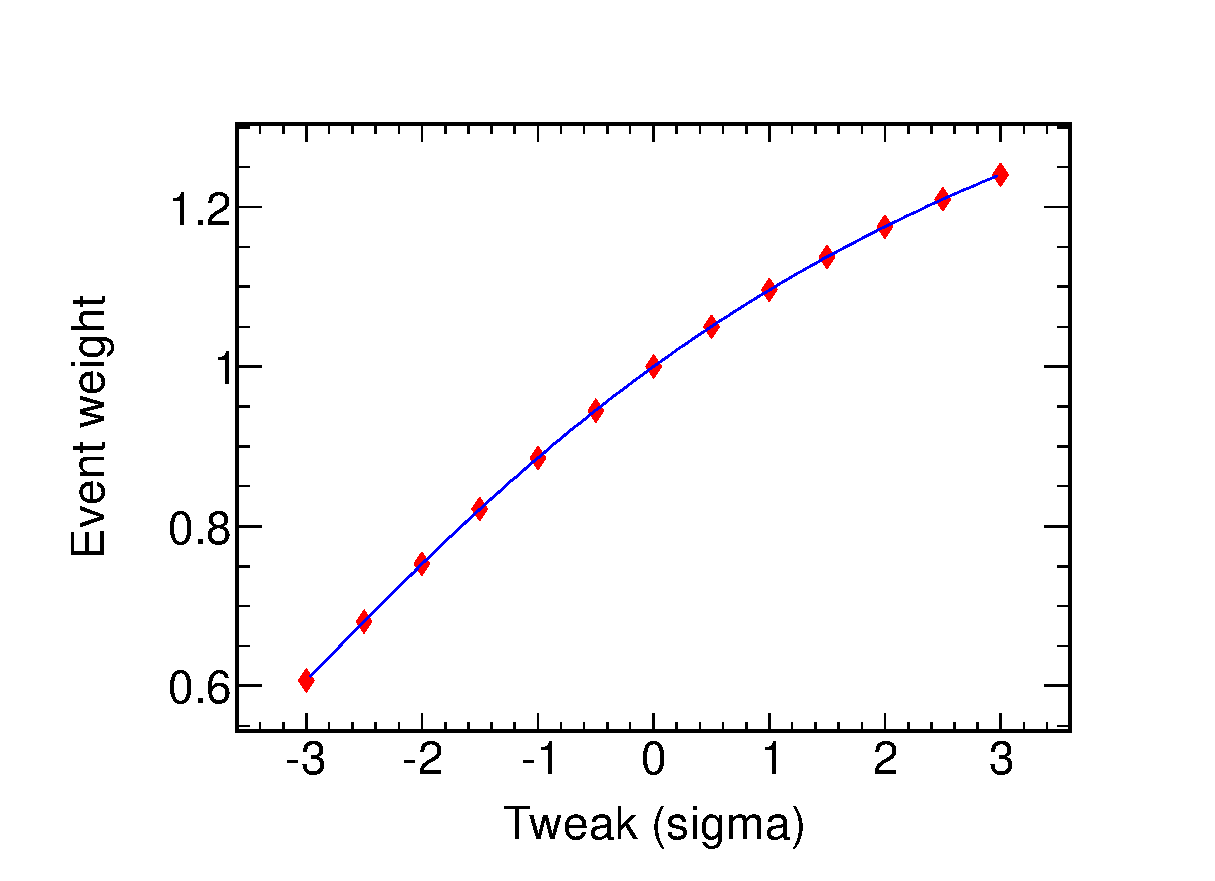
\includegraphics[width=25pc]{./images/spectrum_tweaked/ExampleSpline}
%
\includegraphics[width=15pc]{./images/placeholder}
%\caption {
%Example of a cross-section spline; this shows the event weights obtained by tweaking $M_{A}^{QE}$
%for $\nu_{\mu}$-CCQE events in the bin with reconstructed energy 0.75-0.8 GeV and 
%true energy 0.6-0.7 GeV.
%}
%\label{fig:example_spline}
%\end{figure}
%
%....................................................................................................................


\subsection {Evaluation of effects of systematic parameters on the predicted single $\mu$-like ring reconstructed energy spectrum}
\label{sec:systematics:evaluation}

In this section, we present the effects of the systematics described in Sec.\ \ref{sec:systematics:inputs}
on the predicted number of single $\mu$-like ring events and the predicted reconstructed energy spectrum in SuperK.
These effects are shown both without oscillations and with oscillations with
$\sin^{2}\theta_{23}$ = 0.5 and $|\Delta m^{2}_{32}|$ = 2.4$\times$10$^{-3}$ eV$^{2}$/c$^{4}$, the values shown in Tab.\
\ref{tab:pdg2012non23} for $\sin^{2}\theta_{13}$, $\sin^{2}\theta_{12}$ and $\Delta m^{2}_{21}$,
and $\delta_{CP}$=0. The normal mass hierarchy is assumed.
All results are generated for an integrated exposure of 6.5700$\times$10$^{20}$ POT and
the BANFF-tuned MC templates are used.

The effects of systematic uncertainties on the predicted number of events are summarised in Tab.\ \ref{tab:nsk_systematic_table_summary}, 
both for no oscillations and for oscillations with the typical parameter values given above.
In this table, systematic parameters are grouped into five categories and all parameter correlations are taken into account.
Percentage uncertainties are given for both the BANFF prefit and postfit errors.
The individual effect of each parameter is also presented in Tab.\ \ref{tab:nsk_systematic_table}, in which the correlations
between parameters are necessarily ignored.

The effects of the combined systematic uncertainties on the reconstructed energy spectrum of single $\mu$-like ring events
is shown in Fig.\ \ref{fig:1Rmu_error_envelope_total} for the typical oscillation scenario used.
This plot shows the total error envelope for the 1 $\mu$-like ring event reconstructed energy spectrum; this is calculated
as the $\pm$1$\sigma$ spread of bin contents from 100k toy MC experiments generated with randomized systematic parameters.
In Fig.\ \ref{fig:1Rmu_error_envelope_total}, all systematic parameters were considered and their correlations were taken
into account.

Figs.\ \ref{fig:1Rmu_error_ratio_to_nominal_unosc} and \ref{fig:1Rmu_error_ratio_to_nominal_osc}
show the effect of the systematic error, relative to the statistical error
at the Run 1-4 exposure, for the no oscillation and oscillation cases respectively.
It can be seen that the statistical error dominates at all energies.

Figs.\ \ref{fig:1Rmu_systematics_spread_by_group_unosc} and \ref{fig:1Rmu_systematics_spread_by_group_osc}
show the effect of the four categories of systematic error,
relative to the total systematic error, for the no oscillation and oscillation cases respectively.
It can be seen that the SuperK detector + FSI + SI and
uncorrelated cross section systematics dominate the oscillation dip region.

Detailed studies showing the effects of individual systematics on the expected number of
single $\mu$-like ring events are shown in \cite{OurRun1234DisappAnalysisSupplement}.

The individual effect of each systematic parameter on the best-fit values of $\sin^{2}\theta_{23}$ and $|\Delta m^{2}_{32}|$ 
for the normal hierarchy was quantified by making a toy MC experiment with no statistical fluctuations and a +1$\sigma$ tweak of a 
single systematic parameter. A fit for only $\sin^2\theta_{23}$ and $|\Delta m^2_{32}|$, with systematics fixed
are their nominal values,
was made of that experiment, and the +1$\sigma$ effect of that systematic parameter on the 
best-fit values of $\sin^{2}\theta_{23}$ and $|\Delta m^{2}_{32}|$ was taken to be the difference between the best-fit values from 
the experiment with the +1$\sigma$ tweak and an experiment with nominal values of the systematics. Similarly, the -1$\sigma$ effect of that 
parameter was the difference between the best-fit values from an experiment with a -1$\sigma$ tweak and an experiment with 
nominal values of the systematics. This procedure was repeated for each systematic parameter in turn.
For systematic parameters which are correlated, this procedure was repeated twice, both respecting and ignoring correlations.
The study is repeated at multiple input points in the $\sin^{2}\theta_{23}$-$|\Delta m^{2}_{32}|$ plane.

An estimate of the order of the effect of systematics is given in Tabs.\ \ref{tab:star_summary_by_mixing} and
\ref{tab:star_summary_by_mass}, ordered by the effect on $\sin^2\theta_{23}$ and $|\Delta m^2_{32}|$ respectively.
To make this estimate, the systematic effect is compared with the statistical error for the
specific values of $\sin^2\theta_{23}$ and $|\Delta m^2_{32}|$.
The statistical error was evaluated using 10k toy MC datasets with no systematic fluctuations at each input point, 
with each dataset being fitted for only $\sin^\theta_{23}$ and $|\Delta m^2_{32}|$.
For each systematic, the largest effect seen in the study is given, 
whether that is from +1$\sigma$ or -1$\sigma$, including or neglecting correlations,
and from any true values of $\sin^{2}\theta_{23}$ and $|\Delta m^{2}_{32}|$ in the study.


% ..................

\begin{table}[htb]
\centering
\begin{tabular}{| c | D{.}{.}{-1} | D{.}{.}{-1} |}
\hline
%  {\bf Source of uncertainty}    & \multicolumn{1}{c|}{{\bf ${\delta}N_{SK}$/$N_{SK}$}} & \multicolumn{1}{c|}{{\bf ${\delta}N_{SK}$/$N_{SK}$}}\\
  {\bf Source of uncertainty}    & \multicolumn{1}{c|}{{\bf ${\delta}N_{SK}$/$ <N_{SK} >$}} & \multicolumn{1}{c|}{{\bf ${\delta}N_{SK}$/$<N_{SK}>$}}\\
                                 & \multicolumn{1}{c|}{($\beta=0$)} & \multicolumn{1}{c|}{($\beta=1$)}\\
\hline
  SuperK detector    				& 5.05\%                         & 3.03\%                        \\
  FSI + SI + PN 					& 4.34\%				& 2.45\%			\\
  SuperK detector + FSI + SI + PN     & 6.66\%                         & 3.90\%                        \\
\hline
  BANFF (prefit)                 &  12.37\%                        & 12.91\%                       \\
  BANFF (postfit)                & 9.72\%                         & 10.29\%                        \\
\hline
  BANFF (Non-oxygen, postfit)    	& 3.40\%         	         & 3.02\%                        \\
  BANFF (Oxygen-specific postfit) 	& 9.24\%                    & 10.14\%                        \\
  MEC (Oxygen-specific postfit)	   	& 8.86\%                        	 & 9.28\%                        \\
\hline
  Oscillation parameters         & 4.72\%                         & 13.38\%                       \\
\hline
  Total (BANFF prefit)           &  14.96\%                        & 18.60\%                       \\
  Total (BANFF postfit)          & 12.75\%                         & 17.21\%                       \\
\hline
\end{tabular}
\caption{
 Effect of 1$\sigma$ variations of the groups of systematics parameters on total number of
 1-ring electron-like events in the reverse-horn current sample.
 The BANFF parameters considered to be oxygen-specific are Oxygen MEC normalisation, Fermi Energy, Binding Energy, CC Coherent Normalisation,
 NC Coherent normalization and the nue/numu normalisation. 
The effect of each group of systematics is computed as the standard deviation divided by the mean of the distribution
of the total number of superK events.
\NumToys are performed.
% \newline
%{\bf TO UPDATE}
%\newline
}
\label{tab:nsk_systematic_table_summary}
\end{table}


%..................

\begin{table}
\centering
\begin{tabular}{| c || D{.}{.}{-1} | D{.}{.}{-1} || D{.}{.}{-1} | D{.}{.}{-1} |}
\hline
  Source of uncertainty        &  \multicolumn {2}{c||}{${\delta}N_{SK}$/$N_{SK}$} & \multicolumn {2}{c|}{${\delta}N_{SK}$/$N_{SK}$} \\
                               &  \multicolumn {2}{c||}{(no oscillation)}          & \multicolumn {2}{c|}{(oscillations with typical params)} \\
                               & \multicolumn {1}{c|}{BANFF prefit} & \multicolumn {1}{c||}{BANFF postfit} & \multicolumn {1}{c|}{BANFF prefit} & \multicolumn {1}{c|}{BANFF postfit} \\
\hline
               $f_{E; r}^{SK}$ &               0 &               0 &               0 &               0  \\   
           $f_{0; r}^{SK+FSI}$ &            0.09 &           0.098 &            0.15 &            0.18  \\   
           $f_{1; r}^{SK+FSI}$ &             1.8 &             1.9 &            0.68 &            0.74  \\   
           $f_{2; r}^{SK+FSI}$ &             0.4 &            0.43 &            0.92 &             1.0  \\   
           $f_{3; r}^{SK+FSI}$ &             2.4 &             2.1 &             4.6 &             4.0  \\   
           $f_{4; r}^{SK+FSI}$ &           0.017 &           0.016 &            0.25 &            0.27  \\   
           $f_{5; r}^{SK+FSI}$ &             1.1 &             0.9 &             3.8 &             3.2  \\   
\hline
         $f_{0; t, r}^{banff}$ &            0.36 &            0.27 &            0.85 &            0.66  \\   
         $f_{1; t, r}^{banff}$ &             1.0 &            0.74 &            0.67 &             0.5  \\   
         $f_{2; t, r}^{banff}$ &             1.9 &             1.3 &            0.12 &           0.085  \\   
         $f_{3; t, r}^{banff}$ &             2.3 &             1.6 &             0.3 &            0.22  \\   
         $f_{4; t, r}^{banff}$ &             3.4 &             2.4 &             2.2 &             1.6  \\   
         $f_{5; t, r}^{banff}$ &             1.0 &            0.66 &             1.8 &             1.2  \\   
         $f_{6; t, r}^{banff}$ &            0.63 &            0.39 &             1.7 &             1.1  \\   
         $f_{7; t, r}^{banff}$ &            0.33 &             0.2 &             1.0 &            0.65  \\   
         $f_{8; t, r}^{banff}$ &            0.41 &            0.22 &             1.3 &            0.74  \\   
         $f_{9; t, r}^{banff}$ &            0.19 &           0.077 &            0.65 &            0.27  \\   
        $f_{10; t, r}^{banff}$ &           0.051 &           0.019 &            0.17 &           0.066  \\   
        $f_{11; t, r}^{banff}$ &           0.061 &            0.05 &           0.035 &            0.03  \\   
        $f_{12; t, r}^{banff}$ &           0.061 &           0.049 &           0.049 &            0.04  \\   
        $f_{13; t, r}^{banff}$ &           0.085 &           0.067 &            0.16 &            0.13  \\   
        $f_{14; t, r}^{banff}$ &             0.1 &            0.08 &            0.27 &            0.22  \\   
        $f_{15; t, r}^{banff}$ &           0.078 &            0.06 &            0.25 &             0.2  \\   
        $f_{16; t, r}^{banff}$ &            25.0 &             3.4 &            18.0 &             2.8  \\   
        $f_{17; t, r}^{banff}$ &             2.8 &             1.1 &             6.7 &             2.4  \\   
        $f_{18; t, r}^{banff}$ &             7.9 &             5.9 &             4.2 &             3.3  \\   
        $f_{19; t, r}^{banff}$ &             1.4 &            0.55 &             3.9 &             1.6  \\   
        $f_{20; t, r}^{banff}$ &            0.36 &            0.16 &             1.2 &            0.53  \\   
        $f_{21; t, r}^{banff}$ &             3.7 &             1.5 &             4.9 &             2.0  \\   
        $f_{22; t, r}^{banff}$ &             1.7 &            0.47 &             5.4 &             1.6  \\   
\hline
                $f_{pF; t, r}$ &           0.063 &           0.065 &            0.13 &            0.13  \\   
                $f_{SF; t, r}$ &            0.82 &            0.82 &            0.24 &            0.26  \\   
            $f_{Wshape; t, r}$ &            0.12 &           0.072 &             0.4 &            0.26  \\   
        $f_{CCothShape; t, r}$ &            0.28 &             0.3 &            0.78 &            0.89  \\   
    $f_{\pi-less\Delta; t, r}$ &             3.2 &             2.6 &             5.6 &             4.5  \\   
             $f_{bindE; t, r}$ &             0.5 &            0.43 &            0.24 &             0.2  \\   
                $f_{CCcoh; t}$ &            0.54 &            0.58 &            0.81 &            0.93  \\   
           $f_{NC1\pi^\pm; t}$ &            0.31 &            0.21 &             1.1 &            0.75  \\   
                $f_{NCoth; t}$ &            0.25 &            0.24 &            0.85 &            0.85  \\   
              $f_{CC\nu_e; t}$ &         0.00051 &          0.0005 &          0.0077 &          0.0081  \\   
          $f_{CC\bar{\nu}; t}$ &            0.61 &            0.61 &             1.2 &             1.2  \\   
\hline
         $\sin^2(\theta_{13})$ &               0 &               0 &           0.070 &           0.078  \\   
         $\sin^2(\theta_{12})$ &               0 &               0 &           0.040 &           0.036  \\   
             $\Delta m^2_{21}$ &               0 &               0 &           0.027 &           0.025  \\   
                 $\delta_{CP}$ &               0 &               0 &            0.21 &            0.19  \\   

 


\hline
\end{tabular}
\caption{
  Effects of 1$\sigma$ systematic parameter variations on
  the number of 1 $\mu$-like ring events,
  computed
  for no oscillations and
  for oscillations with
  $\sin^{2}\theta_{23}$=0.5, $|\Delta m^{2}_{32}|$=2.4$\times$10$^{-3}$ eV$^{2}$/c$^{4}$, the values shown in Tab.\
  \ref{tab:pdg2012non23} for $\sin^{2}\theta_{13}$, $\sin^{2}\theta_{12}$ and $\Delta m^{2}_{21}$,
  and $\delta_{CP}$=0. Correlations are ignored for this table. The normal mass hierarchy is assumed.
  The numbers shown were calculated for an exposure of 6.5700$\times$10$^{20}$ POT and BANFF-tuned MC templates were used.
}
\label{tab:nsk_systematic_table}
\end{table}


%..................

\begin{figure*}[htb]
\center
\includegraphics[width=30pc]{{./images/spectrum_tweaked/all_envelope_per_50MeV_sinsqtheta12_0.312,13_0.025,23_0.500,dcp_0.000,dmsq_Normal12_0.00007500,23_0.002400eV2}.eps}
\caption {
  Total error envelope of the 1 $\mu$-like ring event reconstructed energy spectrum,
  for oscillations with
  $\sin^{2}\theta_{23}$=0.5 and $|\Delta m^{2}_{32}|$=2.4$\times$10$^{-3}$ eV$^{2}$/c$^{4}$, the values shown in 
  Tab.\ \ref{tab:pdg2012non23} for $\sin^{2}\theta_{13}$, $\sin^{2}\theta_{12}$ and $\Delta m^{2}_{21}$,
  and $\delta_{CP}$=0. The normal mass hierarchy is assumed.
  The numbers shown were calculated for an exposure of 6.5700$\times$10$^{20}$ POT.
  BANFF-tuned MC templates were used.
  The error envelope was calculated as the $\pm$1$\sigma$ spread of bin contents using an ensemble of 100k toy MC experiments
  generated with randomized systematic parameters.
  All systematic parameters were considered and their correlations were taken into account.
}
\label{fig:1Rmu_error_envelope_total}
\end{figure*}

%..................

\begin{figure*}[htb]
\begin{minipage}[t]{0.48\linewidth}
\center
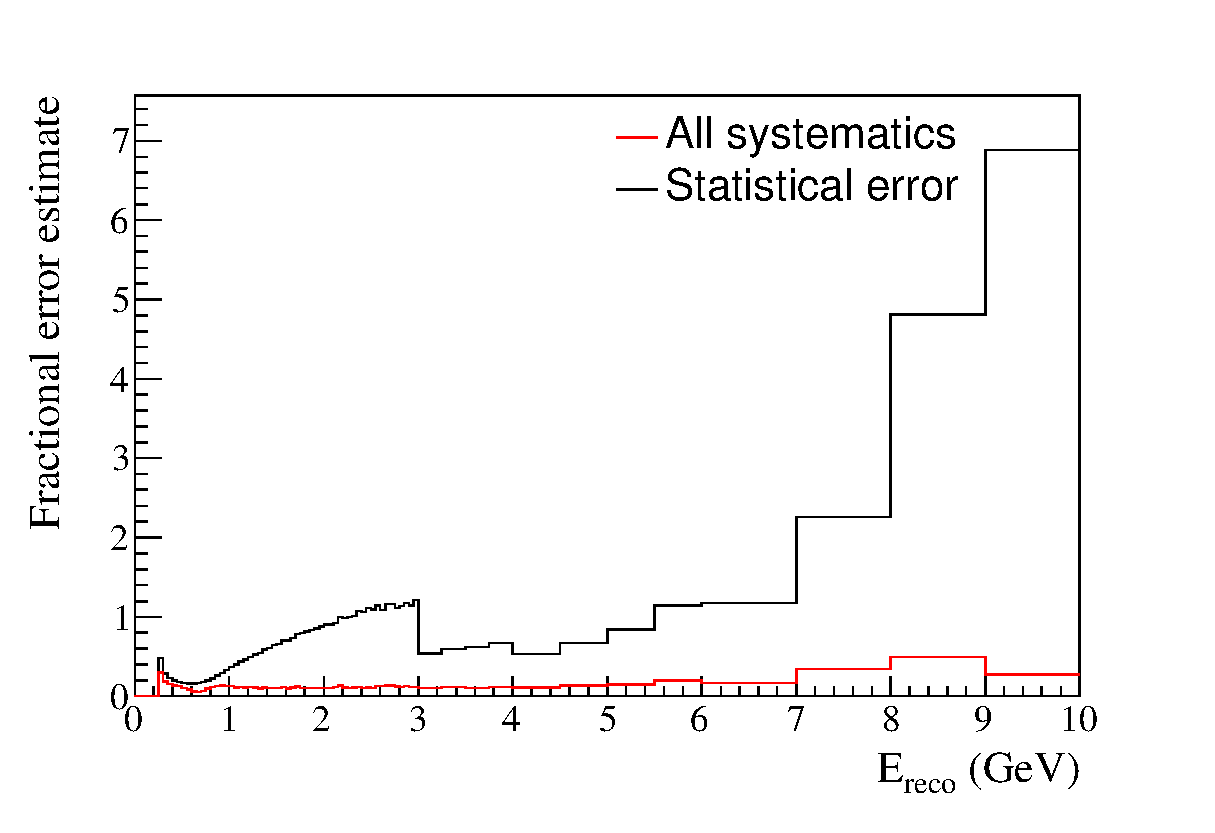
\includegraphics[width=20pc]{./images/spectrum_tweaked/unoscillated_statistical_systematic_sizes.eps}
\caption {
  Comparative size of systematic and statistical error effects per bin.
  100k toy MC experiments were generated with randomized systematic parameters and the 1$\sigma$ spread of bin contents was calculated.
  The fractional systematic error is estimated as the 1$\sigma$ spread divided by the expected number of events in each bin.
  The fractional statistical error is estimated as the inverse square root of the number of events in each bin at 6.5700$\times$10$^{20}$ POT.
  BANFF tuned MC templates were used.
  All systematic parameters were considered and their correlations were taken into account.
  No oscillations were applied.
}
\label{fig:1Rmu_error_ratio_to_nominal_unosc}
\end{minipage}
\hspace{0.06\linewidth}
\begin{minipage}[t]{0.48\linewidth}
\center
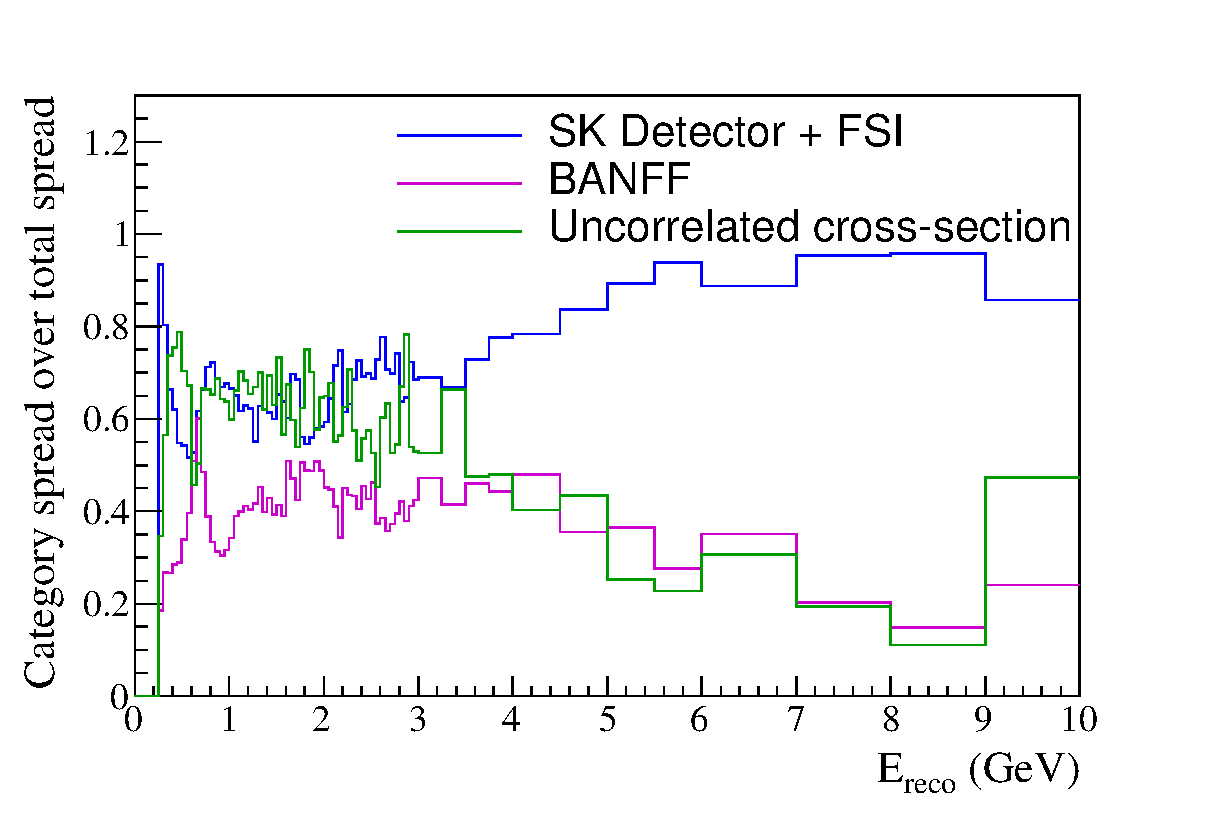
\includegraphics[width=20pc]{./images/spectrum_tweaked/unoscillated_systematic_spread_ratios.eps}
\caption {
  Ratio of event-per-bin 1$\sigma$ spread with individual systematic categories randomized, to the equivalent spread with all systematics randomized.
  100k toy MC experiments each were generated with different groups of systematics randomized, and with all systematics randomized, and the 1$\sigma$ spread of bin contents was calculated.
  BANFF tuned MC templates were used.
  No oscillations were applied.
}
\label{fig:1Rmu_systematics_spread_by_group_unosc}
\end{minipage}
\end{figure*}

\begin{figure*}[htb]
\begin{minipage}[t]{0.48\linewidth}
\center
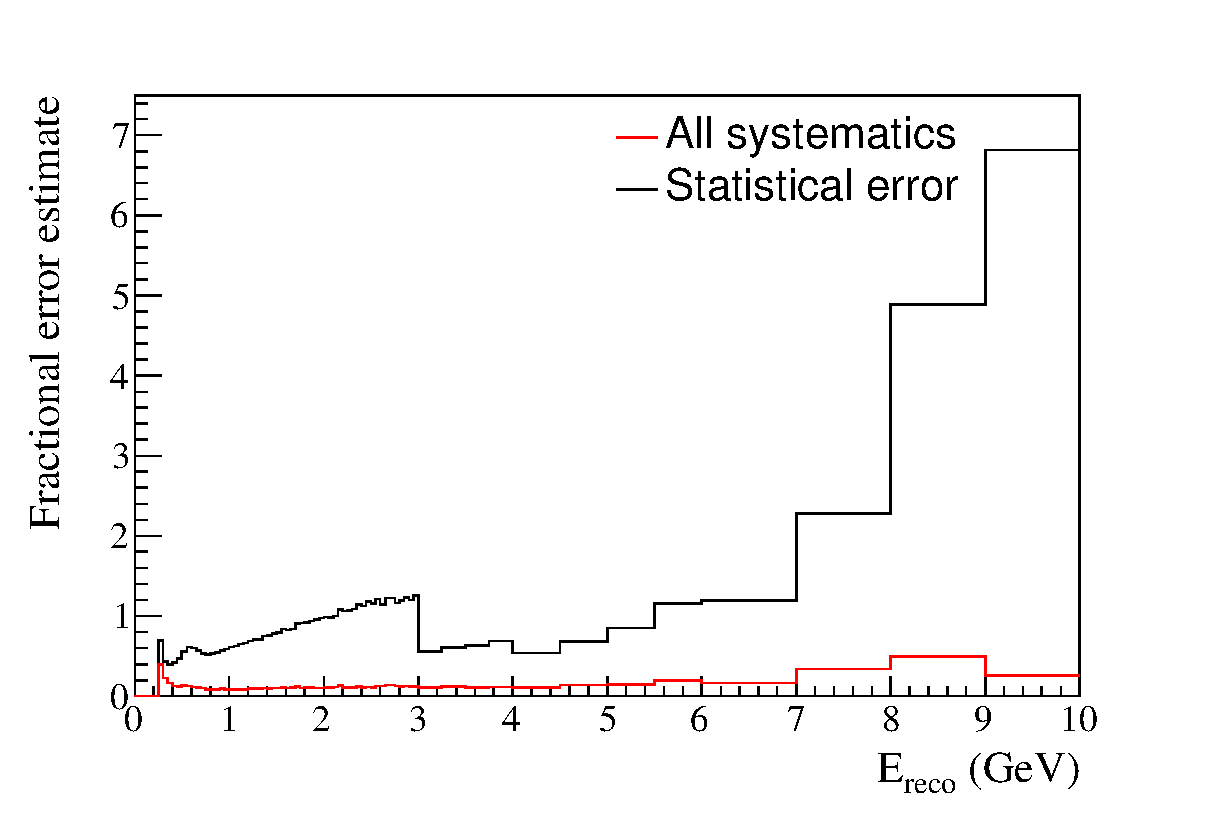
\includegraphics[width=20pc]{./images/spectrum_tweaked/oscillated_statistical_systematic_sizes.eps}
\caption {
  As in Fig. \ref{fig:1Rmu_error_ratio_to_nominal_unosc}, but with oscillations applied for $\sin^{2}\theta_{23}$=0.5, $|\Delta m^{2}_{32}|$=2.4$\times$10$^{-3}$ eV$^{2}$/c$^{4}$, the values shown in
  Tab.\ \ref{tab:pdg2012non23} for $\sin^{2}\theta_{13}$, $\sin^{2}\theta_{12}$ and $\Delta m^{2}_{21}$,
  and $\delta_{CP}$=0. The normal mass hierarchy is assumed. 
}
\label{fig:1Rmu_error_ratio_to_nominal_osc}
\end{minipage}
\hspace{0.06\linewidth}
\begin{minipage}[t]{0.48\linewidth}
\center
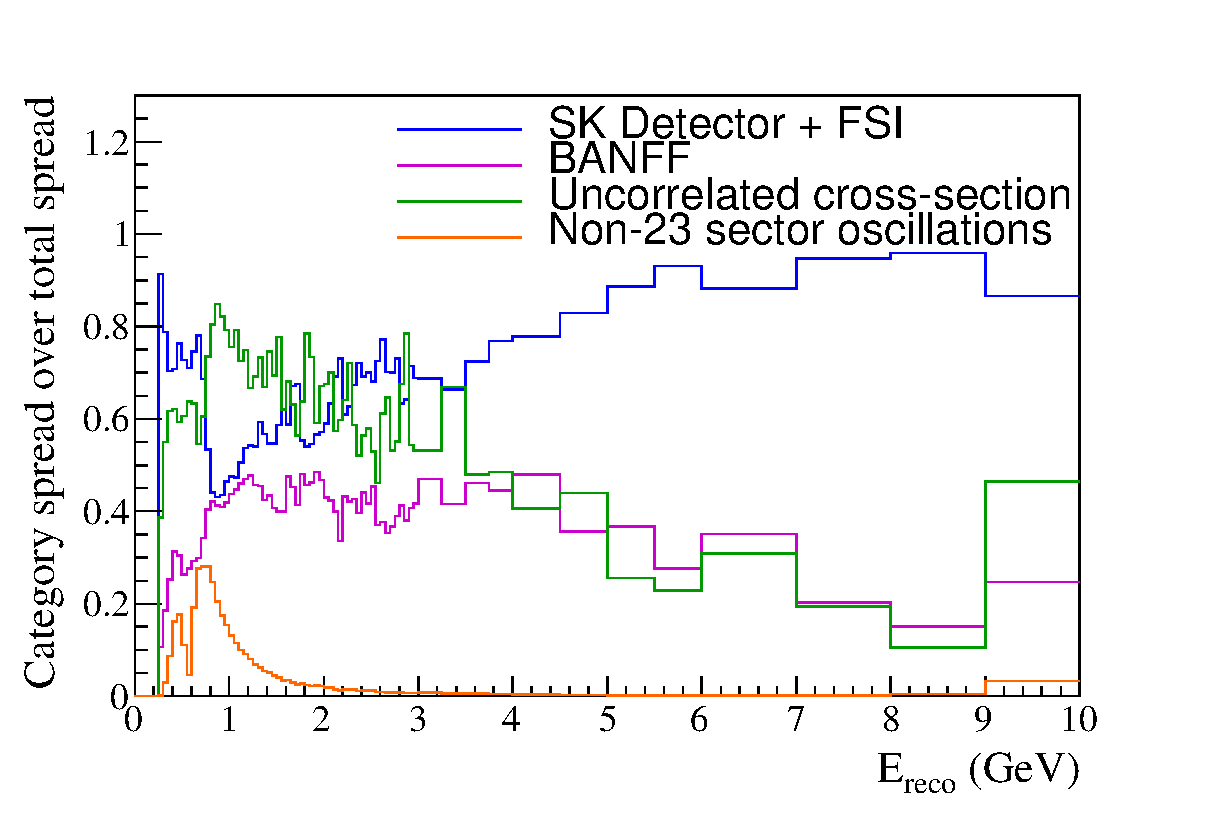
\includegraphics[width=20pc]{./images/spectrum_tweaked/oscillated_systematic_spread_ratios.eps}
\caption {
  As in Fig. \ref{fig:1Rmu_systematics_spread_by_group_unosc}, but with oscillations applied for $\sin^{2}\theta_{23}$=0.5, $|\Delta m^{2}_{32}|$=2.4$\times$10$^{-3}$ eV$^{2}$/c$^{4}$, the values shown in
  Tab.\ \ref{tab:pdg2012non23} for $\sin^{2}\theta_{13}$, $\sin^{2}\theta_{12}$ and $\Delta m^{2}_{21}$,
  and $\delta_{CP}$=0. The normal mass hierarchy is assumed. 
}
\label{fig:1Rmu_systematics_spread_by_group_osc}
\end{minipage}
\end{figure*}

%..................

\begin{table}
\small
\centering
\begin{tabular}{| c | c | c |}
\hline
 Parameter               &  $\frac{\delta_{syst} sin^2\overline{\theta_{23}}}{\delta_{stat} sin^2\overline{\theta_{23}}}$   &  $\frac{\delta_{syst}|\overline{\Delta m^2_{32}}| (eV^{2}/c^{4})}{\delta_{stat} |\overline{\Delta m^2_{32}}| (eV^{2}/c^{4})}$ \\
\hline
                               SKDet + FSI/SI  5; $E_r$ =  0.00 - 30.00 GeV; all NC; RHC & 1.040 & 0.225 \\ \hline 
                                       Meson exchange current normalisation for $^{16}$O & 0.918 & 0.127 \\ \hline 
                                                  CC coherent for $^{16}$O normalisation & 0.491 & 0.028 \\ \hline 
                            C$^{A}_{5}$ nucleon to $\Delta$ transition axial form factor & 0.422 & 0.024 \\ \hline 
                                                                    SK energy scale; RHC & 0.383 & 0.101 \\ \hline 
                                                                  NC other normalisation & 0.347 & 0.029 \\ \hline 
                               RHC $\bar{\nu_\mu}$ flux normalisation, E = 0.7 - 1.0 GeV & 0.326 & 0.048 \\ \hline 
       SKDet + FSI/SI  3; $E_r$ =  0.00 - 30.00 GeV; $\overset{(-)}{\nu_\mu}$ CCnQE; RHC & 0.315 & 0.022 \\ \hline 
                                             Scale of isospin 1/2 nonresonant background & 0.315 & 0.012 \\ \hline 
                                          Resonance-production axial-mass scaling factor & 0.247 & 0.011 \\ \hline 
                                                             Fermi momentum for $^{16}$O & 0.230 & 0.024 \\ \hline 
                               RHC $\bar{\nu_\mu}$ flux normalisation, E = 0.0 - 0.4 GeV & 0.228 & 0.021 \\ \hline 
         SKDet + FSI/SI  1; $E_r$ =  0.40 - 1.10 GeV; $\overset{(-)}{\nu_\mu}$ CCQE; RHC & 0.225 & 0.023 \\ \hline 
            SKDet + FSI/SI  4; $E_r$ =  0.00 - 30.00 GeV; $\overset{(-)}{\nu_e}$ CC; RHC & 0.211 & 0.009 \\ \hline 
                               RHC $\bar{\nu_\mu}$ flux normalisation, E = 1.0 - 1.5 GeV & 0.202 & 0.016 \\ \hline 
                                                          CCQE axial-mass scaling factor & 0.200 & 0.021 \\ \hline 
                               RHC $\bar{\nu_\mu}$ flux normalisation, E = 0.4 - 0.5 GeV & 0.190 & 0.030 \\ \hline 
                                     RHC $\nu_\mu$ flux normalisation, E = 1.0 - 1.5 GeV & 0.150 & 0.009 \\ \hline 
                               RHC $\bar{\nu_\mu}$ flux normalisation, E = 0.6 - 0.7 GeV & 0.142 & 0.009 \\ \hline 
         SKDet + FSI/SI  0; $E_r$ =  0.00 - 0.40 GeV; $\overset{(-)}{\nu_\mu}$ CCQE; RHC & 0.116 & 0.006 \\ \hline 
                               RHC $\bar{\nu_\mu}$ flux normalisation, E = 0.5 - 0.6 GeV & 0.115 & 0.025 \\ \hline 
                                     RHC $\nu_\mu$ flux normalisation, E = 0.7 - 1.0 GeV & 0.113 & 0.006 \\ \hline 
                               RHC $\bar{\nu_\mu}$ flux normalisation, E = 1.5 - 2.5 GeV & 0.108 & 0.005 \\ \hline 
                                     RHC $\nu_\mu$ flux normalisation, E = 0.0 - 0.7 GeV & 0.100 & 0.009 \\ \hline 
                                                                          CC other shape & 0.096 & 0.003 \\ \hline 
                                     RHC $\nu_\mu$ flux normalisation, E = 1.5 - 2.5 GeV & 0.087 & 0.006 \\ \hline 
                                    RHC $\nu_\mu$ flux normalisation, E = 2.5 - 30.0 GeV & 0.085 & 0.004 \\ \hline 
        SKDet + FSI/SI  2; $E_r$ =  1.10 - 30.00 GeV; $\overset{(-)}{\nu_\mu}$ CCQE; RHC & 0.070 & 0.005 \\ \hline 
                                                             Binding energy for $^{16}$O & 0.063 & 0.007 \\ \hline 
                               RHC $\bar{\nu_\mu}$ flux normalisation, E = 2.5 - 3.5 GeV & 0.051 & 0.001 \\ \hline 
                               RHC $\bar{\nu_\mu}$ flux normalisation, E = 3.5 - 5.0 GeV & 0.021 & 0.002 \\ \hline 
                                                               NC coherent normalisation & 0.019 & 0.000 \\ \hline 
                              RHC $\bar{\nu_\mu}$ flux normalisation, E = 7.0 - 30.0 GeV & 0.009 & 0.000 \\ \hline 
                                                              CC $\nu_{e}$ normalisation & 0.008 & 0.000 \\ \hline 
                               RHC $\bar{\nu_\mu}$ flux normalisation, E = 5.0 - 7.0 GeV & 0.007 & 0.000 \\ \hline 
                                      RHC $\nu_e$ flux normalisation, E = 2.5 - 30.0 GeV & 0.006 & 0.000 \\ \hline 
                                       RHC $\nu_e$ flux normalisation, E = 0.0 - 2.5 GeV & 0.004 & 0.000 \\ \hline 
                                RHC $\bar{\nu_e}$ flux normalisation, E = 4.0 - 30.0 GeV & 0.003 & 0.000 \\ \hline 
                                 RHC $\bar{\nu_e}$ flux normalisation, E = 2.5 - 4.0 GeV & 0.002 & 0.000 \\ \hline 
                                 RHC $\bar{\nu_e}$ flux normalisation, E = 1.5 - 2.5 GeV & 0.001 & 0.000 \\ \hline 
                                 RHC $\bar{\nu_e}$ flux normalisation, E = 0.8 - 1.5 GeV & 0.000 & 0.000 \\ \hline 
                                 RHC $\bar{\nu_e}$ flux normalisation, E = 0.5 - 0.7 GeV & 0.000 & 0.000 \\ \hline 
                                 RHC $\bar{\nu_e}$ flux normalisation, E = 0.0 - 0.5 GeV & 0.000 & 0.000 \\ \hline 
                                 RHC $\bar{\nu_e}$ flux normalisation, E = 0.7 - 0.8 GeV & 0.000 & 0.000 \\ \hline 
                            
\hline
\end{tabular}
\caption{
  Maximum deviations, as a fraction of statistical error at the oscillation
  parameter grid point, from the input values of fits for only $\sin^2\overline{\theta_{23}}$ and $|\overline{\Delta m^2_{32}}|$ to datasets with 
  $\pm$1 sigma individual systematic variations at a range of 23-sector oscillation points.
  $|\overline{\Delta m^2_{32}}|$ values of
  2.0$\times$10$^{-3}$ eV$^{2}$/c$^{4}$,
  2.5$\times$10$^{-3}$ eV$^{2}$/c$^{4}$, and
  3.0$\times$10$^{-3}$ eV$^{2}$/c$^{4}$
  are used with each of
  $\sin^2\overline{\theta_{23}} = $ 
  0.370, 0.500, 0.524, 0.650.
  All other oscillation parameters are fixed at the values in table~\ref{tab:osc_params_fixed_values_reactor}.
  These maximum deviations usually occur at maximum disappearance, where the statistical error is smaller, as explained in
  Sec.~\ref{sec:validation}. The values are sorted by the size of the deviation in $\sin^2\overline{\theta_{23}}$.
}
\label{tab:star_summary_by_mixing}
\end{table}

\begin{table}
\small
\centering
\begin{tabular}{| c | c | c |}
\hline
 Parameter               &  $\frac{\delta_{syst} sin^2\overline{\theta_{23}}}{\delta_{stat} sin^2\overline{\theta_{23}}}$   &  $\frac{\delta_{syst}|\overline{\Delta m^2_{32}}| (eV^{2}/c^{4})}{\delta_{stat} |\overline{\Delta m^2_{32}}| (eV^{2}/c^{4})}$ \\
\hline
                                      SKDet + FSI/SI  5; $E_r$ =  0.00 - 30.00 GeV; all NC; RHC & 1.040 & 0.225 \\ \hline 
                                              Meson exchange current normalisation for $^{16}$O & 0.918 & 0.127 \\ \hline 
                                                                           SK energy scale; RHC & 0.383 & 0.101 \\ \hline 
                                      RHC $\bar{\nu_\mu}$ flux normalisation, E = 0.7 - 1.0 GeV & 0.326 & 0.048 \\ \hline 
                                      RHC $\bar{\nu_\mu}$ flux normalisation, E = 0.4 - 0.5 GeV & 0.190 & 0.030 \\ \hline 
                                                                         NC other normalisation & 0.347 & 0.029 \\ \hline 
                                                         CC coherent for $^{16}$O normalisation & 0.491 & 0.028 \\ \hline 
                                      RHC $\bar{\nu_\mu}$ flux normalisation, E = 0.5 - 0.6 GeV & 0.115 & 0.025 \\ \hline 
                                   C$^{A}_{5}$ nucleon to $\Delta$ transition axial form factor & 0.422 & 0.024 \\ \hline 
                                                                    Fermi momentum for $^{16}$O & 0.230 & 0.024 \\ \hline 
                SKDet + FSI/SI  1; $E_r$ =  0.40 - 1.10 GeV; $\overset{(-)}{\nu_\mu}$ CCQE; RHC & 0.225 & 0.023 \\ \hline 
              SKDet + FSI/SI  3; $E_r$ =  0.00 - 30.00 GeV; $\overset{(-)}{\nu_\mu}$ CCnQE; RHC & 0.315 & 0.022 \\ \hline 
                                                                 CCQE axial-mass scaling factor & 0.200 & 0.021 \\ \hline 
                                      RHC $\bar{\nu_\mu}$ flux normalisation, E = 0.0 - 0.4 GeV & 0.228 & 0.021 \\ \hline 
                                      RHC $\bar{\nu_\mu}$ flux normalisation, E = 1.0 - 1.5 GeV & 0.202 & 0.016 \\ \hline 
                                                    Scale of isospin 1/2 nonresonant background & 0.315 & 0.012 \\ \hline 
                                                 Resonance-production axial-mass scaling factor & 0.247 & 0.011 \\ \hline 
                                      RHC $\bar{\nu_\mu}$ flux normalisation, E = 0.6 - 0.7 GeV & 0.142 & 0.009 \\ \hline 
                   SKDet + FSI/SI  4; $E_r$ =  0.00 - 30.00 GeV; $\overset{(-)}{\nu_e}$ CC; RHC & 0.211 & 0.009 \\ \hline 
                                            RHC $\nu_\mu$ flux normalisation, E = 0.0 - 0.7 GeV & 0.100 & 0.009 \\ \hline 
                                            RHC $\nu_\mu$ flux normalisation, E = 1.0 - 1.5 GeV & 0.150 & 0.009 \\ \hline 
                                                                    Binding energy for $^{16}$O & 0.063 & 0.007 \\ \hline 
                                            RHC $\nu_\mu$ flux normalisation, E = 1.5 - 2.5 GeV & 0.087 & 0.006 \\ \hline 
                SKDet + FSI/SI  0; $E_r$ =  0.00 - 0.40 GeV; $\overset{(-)}{\nu_\mu}$ CCQE; RHC & 0.116 & 0.006 \\ \hline 
                                            RHC $\nu_\mu$ flux normalisation, E = 0.7 - 1.0 GeV & 0.113 & 0.006 \\ \hline 
                                      RHC $\bar{\nu_\mu}$ flux normalisation, E = 1.5 - 2.5 GeV & 0.108 & 0.005 \\ \hline 
               SKDet + FSI/SI  2; $E_r$ =  1.10 - 30.00 GeV; $\overset{(-)}{\nu_\mu}$ CCQE; RHC & 0.070 & 0.005 \\ \hline 
                                           RHC $\nu_\mu$ flux normalisation, E = 2.5 - 30.0 GeV & 0.085 & 0.004 \\ \hline 
                                                                                 CC other shape & 0.096 & 0.003 \\ \hline 
                                      RHC $\bar{\nu_\mu}$ flux normalisation, E = 3.5 - 5.0 GeV & 0.021 & 0.002 \\ \hline 
                                      RHC $\bar{\nu_\mu}$ flux normalisation, E = 2.5 - 3.5 GeV & 0.051 & 0.001 \\ \hline 
                                      RHC $\bar{\nu_\mu}$ flux normalisation, E = 5.0 - 7.0 GeV & 0.007 & 0.000 \\ \hline 
                                                                      NC coherent normalisation & 0.019 & 0.000 \\ \hline 
                                     RHC $\bar{\nu_\mu}$ flux normalisation, E = 7.0 - 30.0 GeV & 0.009 & 0.000 \\ \hline 
                                                                     CC $\nu_{e}$ normalisation & 0.008 & 0.000 \\ \hline 
                                             RHC $\nu_e$ flux normalisation, E = 2.5 - 30.0 GeV & 0.006 & 0.000 \\ \hline 
                                              RHC $\nu_e$ flux normalisation, E = 0.0 - 2.5 GeV & 0.004 & 0.000 \\ \hline 
                                        RHC $\bar{\nu_e}$ flux normalisation, E = 2.5 - 4.0 GeV & 0.002 & 0.000 \\ \hline 
                                       RHC $\bar{\nu_e}$ flux normalisation, E = 4.0 - 30.0 GeV & 0.003 & 0.000 \\ \hline 
                                        RHC $\bar{\nu_e}$ flux normalisation, E = 1.5 - 2.5 GeV & 0.001 & 0.000 \\ \hline 
                                        RHC $\bar{\nu_e}$ flux normalisation, E = 0.0 - 0.5 GeV & 0.000 & 0.000 \\ \hline 
                                        RHC $\bar{\nu_e}$ flux normalisation, E = 0.5 - 0.7 GeV & 0.000 & 0.000 \\ \hline 
                                        RHC $\bar{\nu_e}$ flux normalisation, E = 0.7 - 0.8 GeV & 0.000 & 0.000 \\ \hline 
                                        RHC $\bar{\nu_e}$ flux normalisation, E = 0.8 - 1.5 GeV & 0.000 & 0.000 \\ \hline 
\hline
\end{tabular}
\caption{
  Maximum deviations, as a fraction of statistical error at the oscillation
  parameter grid point, from the input values of fits for only $\sin^2\overline{\theta_{23}}$ and $|\overline{\Delta m^2_{32}}|$ to datasets with 
  $\pm$1 sigma individual systematic variations at a range of 23-sector oscillation points.
  $|\overline{\Delta m^2_{32}}|$ values of
  2.0$\times$10$^{-3}$ eV$^{2}$/c$^{4}$,
  2.5$\times$10$^{-3}$ eV$^{2}$/c$^{4}$, and
  3.0$\times$10$^{-3}$ eV$^{2}$/c$^{4}$
  are used with each of
  $\sin^2\overline{\theta_{23}} = $ 
  0.370, 0.500, 0.524, 0.650.
  All other oscillation parameters are fixed at the values in table~\ref{tab:osc_params_fixed_values_reactor}.
  These maximum deviations usually occur at maximum disappearance, where the statistical error is smaller, as explained in
  Sec.~\ref{sec:validation}. The values are sorted by the size of the deviation in $|\overline{\Delta m^2_{32}}|$.
}
\label{tab:star_summary_by_mass}
\end{table}


%..................


\clearpage

\section {Neutrino oscillation fitting}
\label{sec:oscfit}

%--------------------------------------------------------------------------------------------------------------------
\subsection {Fit method}
\label{sec:oscfit_method}

Several choices exist for the 23-sector oscillation parameters that could be fitted, 
and these choices have been presented in the context of the {\em VALOR} joint 3-flavour fit of the 1 $\mu$-like ring 
and 1 e-like ring reconstructed SuperK spectra \cite{Lorena}.
During the review process of the T2K Run 1+2+3 $\nu_{\mu}$-disappearance PRL \cite{T2KRun123Disapp}, it was discovered that the
choice of octant ($\theta_{23} \leq \pi/4$ or $\theta_{23} \geq \pi/4$) has a large effect on the confidence contour in $\sin^2(2\theta_{23})$.
Therefore, we now fit $\sin^2\theta_{23}$ by default. This is a sensible choice since the value of $\sin^2\theta_{23}$ giving
 maximal disappearance is not the same as the value giving maximal mixing ($\sin^2\theta_{23}$ = 0.5); this difference is 
due to the non-zero value of $\theta_{13}$.
There are also different choices for the mass-squared splitting parameter: typically $|\Delta m^{2}_{32}|$ is used in $\nu_{\mu}$-disappearance 
analyses, but this is the largest mass-squared splitting for the inverted mass
hierarchy and the second largest for the normal mass hierarchy. 
It is therefore not correct to compare results obtained under the different mass hierarchy hypotheses.
Other choices include fitting a mass-squared difference whose absolute value is the same for both mass hierarchies,
such as $\Delta m^{2} = \left(m_{3}^{2} - \frac {m_{1}^{2}+m_{2}^{2}} {2} \right)$ \cite{FogliLisi},
or fitting $|\Delta m^{2}_{32}|$ for one hierarchy and $|\Delta m^{2}_{31}|$ for the other \cite{GonzalezGarcia}.
All these choices are implemented in the {\em VALOR} oscillation analysis framework, and our analysis can switch between them.
For the present analysis, it was decided to fit 
$|\Delta m^{2}_{32}|$ for the normal hierarchy and $|\Delta m^{2}_{31}|$ for the inverted hierarchy. The actual inputs to the calculation 
of the oscillation probabilities are +$|\Delta m^{2}_{32}|$ for the normal hierarchy and -$|\Delta m^{2}_{31}|$ for the inverted hierarchy.
Fits of $|\Delta m^{2}_{32}|$ for the inverted hierarchy were also performed for validation.

The {\em VALOR} disappearance analysis uses a binned likelihood-ratio method.
Measurements of the oscillation parameters $\sin^{2}\theta_{23}$ and $|\Delta m^{2}_{32}|$ or $|\Delta m^{2}_{31}|$
are obtained by comparing the observed and predicted SuperK reconstructed energy spectra
for 1-ring $\mu$-like events.

Let $N$ be the number of reconstructed energy bins and
${\bf a}$ be a $1 \times N_{s}$ - dimensional array of systematic (nuisance) 
parameters that affect the SuperK reconstructed energy spectrum prediction (e.g
parameters that control the beam, neutrino interaction simulations and 
the detector response).
Best-fit values are obtained by minimizing: 
\begin{equation}
\displaystyle
%\chi^{2} 
-2 \; \textrm{ln} \; \lambda (\sin^{2}\theta_{23},|\Delta m^{2}_{32}| \; \textrm{or} \; |\Delta m^{2}_{31}|; {\bf a}) = 
  2 \cdot \sum_{i=0}^{N-1} 
   \Big( 
     n^{obs}_{i} \cdot ln(n^{obs}_{i}/n^{exp}_{i}) +
     (n^{exp}_{i}-n^{obs}_{i}) 
   \Big) +
   ({\bf a}-{\bf a_{0}})^{T} \cdot {\bf C}^{-1} \cdot ({\bf a}-{\bf a_{0}})
\label{eq:chisquare}
\end{equation}
where
${\bf a_{0}}$ is an $1 \times N_{s}$ - dimensional array with the default values of 
the systematics parameters, ${\bf a}^{T}$ is the transpose of ${\bf a}$,
${\bf C}$ is the systematic parameter covariance matrix of dimension $N_{s} \times N_{s}$,
$n^{obs}_{i}$ is the observed number of events in the $i^{th}$ bin, and
$n^{exp}_{i} = n^{exp}_{i}(\sin^{2}\theta_{23},|\Delta m^{2}_{32}| \; \textrm{or} \; |\Delta m^{2}_{31}|; {\bf a})$ 
is the corresponding expected number of events.

The likelihood-ratio method used in this analysis is equivalent to the extended maximum likelihood
method used in the alternative T2K oscillation analysis 
(see \cite{OurRun1DisappAnalysis,StatAnalysisCowan} for more details).
The advantage of the likelihood ratio method, compared with the extended maximum-likelihood method, is that
in the large-sample limit, the quantity $-2 \: \textrm{ln} \: \lambda (\sin^{2}\theta_{23},|\Delta m^{2}_{32}| \; \textrm{or} \; |\Delta m^{2}_{31}|; {\bf a})$
in Eq.\ref{eq:chisquare} has a $\chi^{2}$ distribution and it can therefore be used as a goodness-of-fit test.
In this note,
$-2 \: \textrm{ln} \: \lambda (\sin^{2}\theta_{23},|\Delta m^{2}_{32}| \; \textrm{or} \; |\Delta m^{2}_{31}|; {\bf a})$ and
$\chi^{2}(\sin^{2}\theta_{23},|\Delta m^{2}_{32}| \; \textrm{or} \; |\Delta m^{2}_{31}|; {\bf a})$ are used interchangeably.

The minimization is performed with Minuit \cite{Minuit}, using the Migrad method.
If Migrad does not converge, the starting values of the oscillation parameters are re-initialised:
the new initial values are randomly drawn from uniform distributions in the ranges 
$1.5 \times 10^{-3}$ eV$^{2}$/c$^{4}$ $\leq$ $|\Delta m^{2}_{32}| \; \textrm{or} \; |\Delta m^{2}_{31}|$ $\leq$ $3.5 \times 10^{-3}$  eV$^{2}$/c$^{4}$ and
either 0.35 $\leq$ $\sin^{2}\theta_{23}$ $\leq$ 0.50 or 0.53 $\leq$ $\sin^{2}\theta_{23}$ $\leq$ 0.68 (the new initial value of 
$\sin^{2}\theta_{23}$ is in the same octant as the previous initial value).  
The fit is retried with the new initial values, and this is repeated up to 10 times.
If the fit still fails to converge after 10 attempts, the Simplex algorithm is used.
The search for the minimum value of 
$-2 \: \textrm{ln} \: \lambda(\sin^{2}\theta_{23},|\Delta m^ {2}_{32}| \; \textrm{or} \; |\Delta m^{2}_{31}|; {\bf a})$ (see Eq. \ref{eq:chisquare}) 
is performed in the range 
$0 \leq$ $\sin^{2}\theta_{23}$ $\leq 1$ and
$1 \times 10^{-3}$ eV$^{2}$/c$^{4}$ $\leq$ $|\Delta m^{2}_{32}| \; \textrm{or} \; |\Delta m^{2}_{31}$ $\leq 6 \times 10^{-3}$ eV$^{2}$/c$^{4}$.
After a successful fit, The Hesse algorithm is called to improve Minuit's estimates of the
errors on the fitted parameters.

Each fit is repeated twice: in the first fit, the initial values are $|\Delta m^{2}_{32}|$ or $|\Delta m^{2}_{31}|$ = 2.4 $\times$ 10$^{-3}$ 
eV$^{2}$/c$^{4}$ and $\sin^{2}\theta_{23} = 0.6$, while the second fit uses as initial values the best fit of $|\Delta m^{2}_{32}|$ or $|\Delta m^{2}_{31}|$ 
and the mirror point in the other octant of the best fit of $\sin^{2}\theta_{23}$ from the first fit. 

All the systematic parameters are allowed to float in the fit, and are restricted to the range [-5$\sigma_{s}$, +5$\sigma_{s}$]
where $\sigma_{s}$ is the one standard deviation error assigned to each systematic parameter\footnote{
 Such an error is defined for all but one of the systematic parameters considered in this analysis. 
 The exception is the systematic parameters $f_{SF}$ which parameterizes the uncertainty on nuclear modelling,
 switching between the Relativistic Fermi Gas (RFG) and Spectral Function (SF) models. The allowed range of the parameter $f_{SF}$ 
 in the oscillation fit is [0,1].}.
Values of systematic parameters that give a negative predicted number of events in any reconstructed energy bin are not allowed. 
If this scenario arises, the number of events is changed to +1E-8 in that bin. This is done for the sum of all the interaction 
modes rather than for each mode separately.

In a 3-flavour $\nu_{\mu}$-disappearance fit, it is also necessary to make a choice for the treatment of the 
non-23-sector oscillation parameters. In the current analysis, we allow each of
$\sin^{2}(2 \theta_{13})$, $\sin^{2}(2 \theta_{12})$, $\Delta m_{21}^{2}$ and $\delta_{CP}$ to float. 
We use penalty terms for $\sin^{2}(2 \theta_{13})$, $\sin^{2}(2 \theta_{12})$, $\Delta m_{21}^{2}$, and their central values 
and uncertainties are shown in Tab.\ \ref{tab:pdg2012non23}; these are taken from the 2012 PDG \cite{PDG2012}\footnote{
  Note that in
  parts of Sec.\ \ref{sec:systematics:evaluation} (Figs.\ \ref{fig:1Rmu_error_ratio_to_nominal_osc}-\ref{fig:1Rmu_systematics_spread_by_group_osc}
  and Tabs.\ \ref{tab:star_summary_by_mixing}-\ref{tab:star_summary_by_mass}),
  Sec.\ \ref{sec:validation},
  and parts of Sec.\ \ref{sec:results} (critical $\Delta\chi^2$ calculatations and Fig.\ \ref{fig:results_compare_constdchisq_sensitivity_normal}),
  a value for $\sin^{2}(\theta_{12})$ of 0.306 with 1$\sigma$ range of 5.9\% \cite{FogliLisi} is used.
  The data best-fit point, 1D limits, and contours are identical using this number.
}.
There is no penalty term for 
$\delta_{CP}$, and it is allowed to float freely in the range [$-\pi$, $+\pi$]\footnote{
 The \emph{non-23-sector} oscillation parameters are allowed to float in the fit in the following ranges:
 $\sin^{2}\theta_{12}$ and $\sin^{2}\theta_{13}$ in the range [0,1];
 $\Delta m^{2}_{21}$ in the range [6,9] $\times 10^{-3} eV^{2}/c^{4}$;
 and $\delta_{CP}$ in the range [$-\pi$, $+\pi$].
}.
\begin{table}
\centering
\begin{tabular}{| c | c | c | }
\hline
Parameter                  &  Best-fit                                    & 1$\sigma$ range  \\
\hline
$\Delta m_{21}^{2}$        &  7.5 $\times$ 10$^{-5}$ eV$^{2}$/c$^{4}$     & $\pm\sim$2.7\% \\
$\sin^{2}(\theta_{12})$    &  0.312                                       & $\pm\sim$5.8\% \\
$\sin^{2}(\theta_{13})$    &  0.0251                                      & $\pm\sim$13.9\% \\
%$\delta_{CP}$              &  -                                           & [-$\pi$,+$\pi$] \\
\hline
\end{tabular}
\caption{
  Best-fit values and 1$\sigma$ range for the measured \emph{non-23-sector} oscillation parameters \cite{PDG2012}.
  $\delta_{CP}$ is allowed to float freely in the range [$-\pi$, $+\pi$] without penalty.
}
\label{tab:pdg2012non23}
\end{table}

%--------------------------------------------------------------------------------------------------------------------

\subsection {Goodness-of-fit tests}
\label{sec:gof_test}

In our $\nu_{\mu}$-disappearance analysis of the Run1+2 datasets, p-values were computed using both 
a) the rate of single $\mu$-like ring events and 
b) the rate and reconstructed energy distribution of single $\mu$-like ring events using the likelihood-ratio method \cite{NickPvalue}.
The choice is not unique.

D. Karlen has pointed out that, if the statistics are low, ``the use of the
distribution is not helpful in forming the p-value. 
This is directly related to the well known problem that is difficult to define
a general goodness-of-fit for sparsely populated distributions.
Large bins (or in the extreme a single bin = rate-only)
are necessary for small statistics samples'' \cite{KarlenPvalue}.

It was decided by the oscillation analysis group that, for all $\nu_{\mu}$-disappearance analyses, 
p-values will be calculated using the rate and the reconstructed energy distribution,
and that the distribution will use a very coarse binning
scheme to ensure that there are sufficient numbers of events in each bin: 
this scheme has 5 bins from 0-0.4, 0.4-0.7, 0.7-1.0, 1.0-2.0 and 2.0-30.0 GeV.

%--------------------------------------------------------------------------------------------------------------------
\subsection {Construction of confidence regions}
\label{sec:contour_construction}

In this analysis, uncertainties in the jointly measured parameters are quoted using both 
the constant-$\Delta\chi^{2}$ \cite{PDG2012} (pp. 390-401)
and the Feldman-Cousins \cite{FeldmanCousins} methods.
A definite recommendation was made in favour of the Feldman and Cousins method 
for constructing confidence regions by the T2K $\nu_{\mu}$ contour committee \cite{T2KNuMuContourCom}.
The work of Feldman and Cousins 
uses the freedom which is inherent in the Neyman construction of confidence regions
to address cases 
(in particular, cases with
Poisson processes with background and Gaussian errors near a physical boundary)
where the classical construction of confidence regions produces overcoverage, undercoverage, or
in extreme cases, an empty region.

The two methods have been described in detail in past T2K technical notes and presentations.
For completeness, we summarise both of these methods here
and provide definite statements on the exact methodology used for incorporating systematic errors.

The methods differ in the calculation of the critical values of $\Delta{\chi^{2}}$, which are used to identify the areas 
of the parameter space to be included in the allowed region for a given confidence level. The constant-$\Delta\chi^{2}$ 
method is a fully frequentist treatment using the Gaussian approximation.
One finds the best-fit point and calculates the confidence contours as lines of \emph{constant} $\Delta{\chi^{2}}$
from this point\footnote{
For 1 fit parameter, the critical values of $\Delta{\chi^{2}}$ used are
1.00 (68\% CL), 2.71 (90\% CL), 3.84 (95\% CL), 6.63 (99\% CL).
For 2 parameters fitted simultaneously, the critical values of $\Delta{\chi^{2}}$ used are
2.30 (68\% CL), 4.61 (90\% CL), 5.99 (95\% CL), 9.21 (99\% CL).
}.

The method of Feldman and Cousins method finds the critical values of $\Delta{\chi^{2}}$ as follows: many toy MC experiment 
fits are performed for each point of the (sin$^{2}\theta_{23}$, $|\Delta$m$^{2}_{32}|$ or $|\Delta$m$^{2}_{31}|$) 2-dimensional grid.
The value of $\Delta\chi^{2}_{MC}$ for each toy MC experiment is calculated as
\begin{equation}
\displaystyle
\Delta \chi^{2}_{MC} = \chi^{2} \textrm{(MC, true)} - \chi^{2} \textrm{(MC, best fit)}
\label{eq:deltachi2mc}
\end{equation}
where
``true'' means that the $\chi^{2}$ was computed using the true values of the oscillation parameters at that grid point, and
``best-fit'' means that the $\chi^{2}$ was computed using the actual best-fit values for that MC experiment.
The $\chi^{2}$ values are calculated using Eq. \ref{eq:chisquare}.
For each grid point, the critical value of $\Delta\chi^{2}$ ($\Delta\chi^{2}_{critical}$)
is found such that $\alpha$ of the toy MC experiments have $\Delta\chi^{2}_{MC}$ $<$ $\Delta\chi^{2}_{critical}$,
where $\alpha$ is the desired confidence level.
%The Feldman and Cousins confidence regions for a fit to an actual dataset are drawn such that grid points 
%with $\Delta\chi^{2}_{data}$ $<$ $\Delta\chi^{2}_{critical}$ are included within the contour, 
%where $\Delta\chi^{2}_{data}$ is given by
%\begin{equation}
%\displaystyle
%\Delta \chi^{2}_{data} = \chi^{2} \textrm{(true)} - \chi^{2} \textrm{(data, best fit)}
%\label{qe:fccontour}
%\end{equation} 
The principal difference between the Feldman and Cousins and the constant $\Delta\chi^{2}$ methods is that the former determines 
the value of $\Delta\chi^{2}_{critical}$ individually for each grid point, whereas the latter uses the same value 
for all grid points.

The procedure for constructing the $\Delta\chi^{2}(\sin^{2}\theta_{23},|\Delta m^{2}_{32}| \; \textrm{or} \; |\Delta m^{2}_{31}|)$
surface itself from the T2K Run 1+2+3+4 data is common to both methods.
Assuming that N nuisance parameters are allowed to float in the oscillation fit,
the values of $\chi^{2}(\sin^{2}\theta_{23},|\Delta m^{2}_{32}| \; \textrm{or} \; |\Delta m^{2}_{31}|; {\bf a})$
are calculated via a fit at \emph{each} point of the (sin$^{2}\theta_{23}$, $|\Delta m^{2}_{32}|$ or $|\Delta m^{2}_{31}|$)
2-dimensional grid, where only the nuisance parameters are allowed to float
and sin$^{2}\theta_{23}$ and $|\Delta$m$^{2}_{32}|$ or $|\Delta m^{2}_{31}|$ are fixed to the true values for the given grid point.
The following grid spacing is used in all confidence region construction methods:
$\delta{\sin^{2}\theta_{23}}=5\times10^{-3}$ and
$\delta |\Delta{m^{2}_{32}}| \; \textrm{or} \; \delta |\Delta m^{2}_{31}|=5\times10^{-5}$ eV$^{2}$/c$^{4}$.

The allowed region in the 2D oscillation parameter space is then given by
\begin{equation}
\displaystyle
\Delta\chi^{2}(\sin^{2}\theta_{23},|\Delta m^{2}_{32}| \textrm{or} |\Delta m^{2}_{31}|) =
\chi^{2}(\sin^{2}\theta_{23},|\Delta m^{2}_{32}| \; \textrm{or} \; |\Delta m^{2}_{31}|; {\bf a}) - \chi_{min}^{2} < \Delta{\chi^{2}}_{critical}
\label{eq:chiconfregion}
\end{equation}
where $\chi_{min}^{2}$ is the minimum value of $\chi^{2}(\sin^{2}\theta_{23},|\Delta m^{2}_{32}| \; \textrm{or} \; |\Delta m^{2}_{31}|; {\bf a})$
from the fit of the T2K Run 1+2+3+4 data over the oscillation parameter space considered.

The Feldman and Cousins method does not specify how systematics are to be included 
in the confidence region construction and different choices exist. 
To construct a 2-dimensional (sin$^{2}$2$\theta_{23}$, $|\Delta m^{2}_{32}|$ or $|\Delta m^{2}_{31}|$) confidence region, 
where N systematic parameters are included in the p.d.f. and all of these N systematics are allowed to float in the fit,
this analysis uses the following methodology: 
the value of $\Delta\chi^{2}_{critical}$ at each true (sin$^{2}\theta_{23}$, $|\Delta m^{2}_{32}|$ or $|\Delta m^{2}_{31}|$) grid point 
is calculated from an ensemble of toy MC experiments,
each one of which is generated with the true oscillation parameters of that point and with all N systematics randomised.
For each toy MC experiment, both sin$^{2}\theta_{23}$, $|\Delta m^{2}_{32}|$ or $|\Delta m^{2}_{31}|$ and all N nuisance parameters are fitted
simultaneously to obtain the value of $\chi^{2} \textrm{(MC, best fit)}$ used in Eq. \ref{eq:deltachi2mc}.
A separate fit, with sin$^{2}\theta_{23}$ and $|\Delta m^{2}_{32}|$ or $|\Delta m^{2}_{31}|$ fixed to their true values
and with all N nuisance parameters allowed to float, is performed to obtain the value of 
$\chi^{2} \textrm{(MC, true)}$ (i.e.\ $\chi^{2}$ is \emph{independently} minimised, for \emph{each} toy MC experiment, with 
respect to the nuisance parameters).

Confidence intervals are also constructed separately for each of sin$^{2}\theta_{23}$ and $|\Delta m^{2}_{32}|$ (normal hierarchy) or 
$|\Delta m^{2}_{31}|$ (inverted hierarchy). 
These can be found in a straightforward way by calculating the 1D profile likelihood for each parameter, and finding the values of 
each parameter corresponding to the constant $\Delta\chi^{2}$ for one parameter and the desired confidence level (e.g.\ 
$\Delta\chi^{2}$ = 1.0 for 68\% C.L.). 
Unfortunately, however, there is no standard procedure in the literature for constructing 1D Feldman-Cousins confidence intervals from 
2D confidence regions. To find the 1D intervals, values of $\Delta{\chi^{2}}_{critical}$ need to be computed, as a function of the 
corresponding oscillation parameter, using an ensemble of toy MC experiments. One issue concerns the choice of the true input value(s) 
of the ``other'' oscillation parameter in those experiments. For example, the true input values of $|\Delta m_{32}^{2}|$ (normal hierarchy) 
or $|\Delta m_{31}^{2}|$ (inverted hierarchy) must be chosen for the toy MC experiment ensemble used for constructing the confidence interval 
in $\sin^2 \theta_{23}$. One option in this case would be to use the T2K Run 1+2+3+4 best-fit value of $|\Delta m_{32}^{2}|$ or $|\Delta m_{31}^{2}|$ 
as the true input value for all the toy MC experiments, but this fails to account for the uncertainty in $|\Delta m_{32}^{2}|$ or 
$|\Delta m_{31}^{2}|$. Alternatively, a uniform distribution of true input values of $|\Delta m_{32}^{2}|$ or $|\Delta m_{31}^{2}|$ could be used 
in some range, say from 2-3$\times$10$^{-3}$ eV$^{2}$/c$^{4}$, but this ignores the fact that some values of $|\Delta m_{32}^{2}|$ 
or $|\Delta m_{31}^{2}|$ are preferred by the T2K data to others.

In this analysis, the true input values of $|\Delta m_{32}^{2}|$ or $|\Delta m_{31}^{2}|$ are chosen using the likelihood from the fit 
of the T2K Run 1+2+3+4 data. At each true value of $\sin^2 \theta_{23}$, the numbers of toy MC experiments with a given true input value 
of $|\Delta m_{32}^{2}|$ or $|\Delta m_{31}^{2}|$ are proportional to e$^{-\frac{\Delta \chi^{2}}{2}}$, where $\Delta \chi^{2}$ is the value 
of the 2-dimensional $\Delta \chi^{2}$ surface at those values of $\sin^2 \theta_{23}$ and $|\Delta m_{32}^{2}|$ or $|\Delta m_{31}^{2}|$ from 
the fit of the T2K Run 1+2+3+4 data. An example of the distribution of true input values of $|\Delta m_{32}^{2}|$ is shown in Fig.\ \ref{fig:input_dm32sq_1DFC}
for a fixed input value of $\sin^2 \theta_{23}$ = 0.55, and an example of the distribution of input values of $\sin^2 \theta_{23}$ for 
an input value of $|\Delta m_{32}^{2}|$ = 2.9$\times$10$^{-3}$ eV$^{2}$/c$^{4}$ is given in Fig.\ \ref{fig:input_mixing23_1DFC}.
Each toy MC experiment is fitted twice; in one fit, $\sin^2 \theta_{23}$, $|\Delta m_{32}^{2}|$ or $|\Delta m_{31}^{2}|$ and all the nuisance 
parameters are allowed to float, and, in the other, $|\Delta m_{32}^{2}|$ or $|\Delta m_{31}^{2}|$ and the nuisance parameters are allowed to 
float while $\sin^2 \theta_{23}$ is fixed to its true value. For each experiment, $\Delta \chi^{2}_{MC}$ is calculated as the difference between 
the minimum values of $\chi^{2}$ from the two fits. The critical value of $\Delta \chi^{2}$ at each true value of $\sin^2 \theta_{23}$ is found 
by combining all the toy MC experiments with that input value of $\sin^2 \theta_{23}$ and different true input values of $|\Delta m_{32}^{2}|$ 
or $|\Delta m_{31}^{2}|$. It is the value of $\Delta \chi^{2}$ such that $\alpha$ of the toy experiments have $\Delta \chi^{2}_{MC}$ $<$ 
$\Delta \chi^{2}_{critical}$, where $\alpha$ is the desired confidence level.

The 1-dimensional Feldman and Cousins confidence intervals in $|\Delta m_{32}^{2}|$ or $|\Delta m_{31}^{2}|$ are constructed in an analogous way. 


\begin{figure*}[htb]
  \begin{minipage}[t]{0.96\linewidth}
    \center
    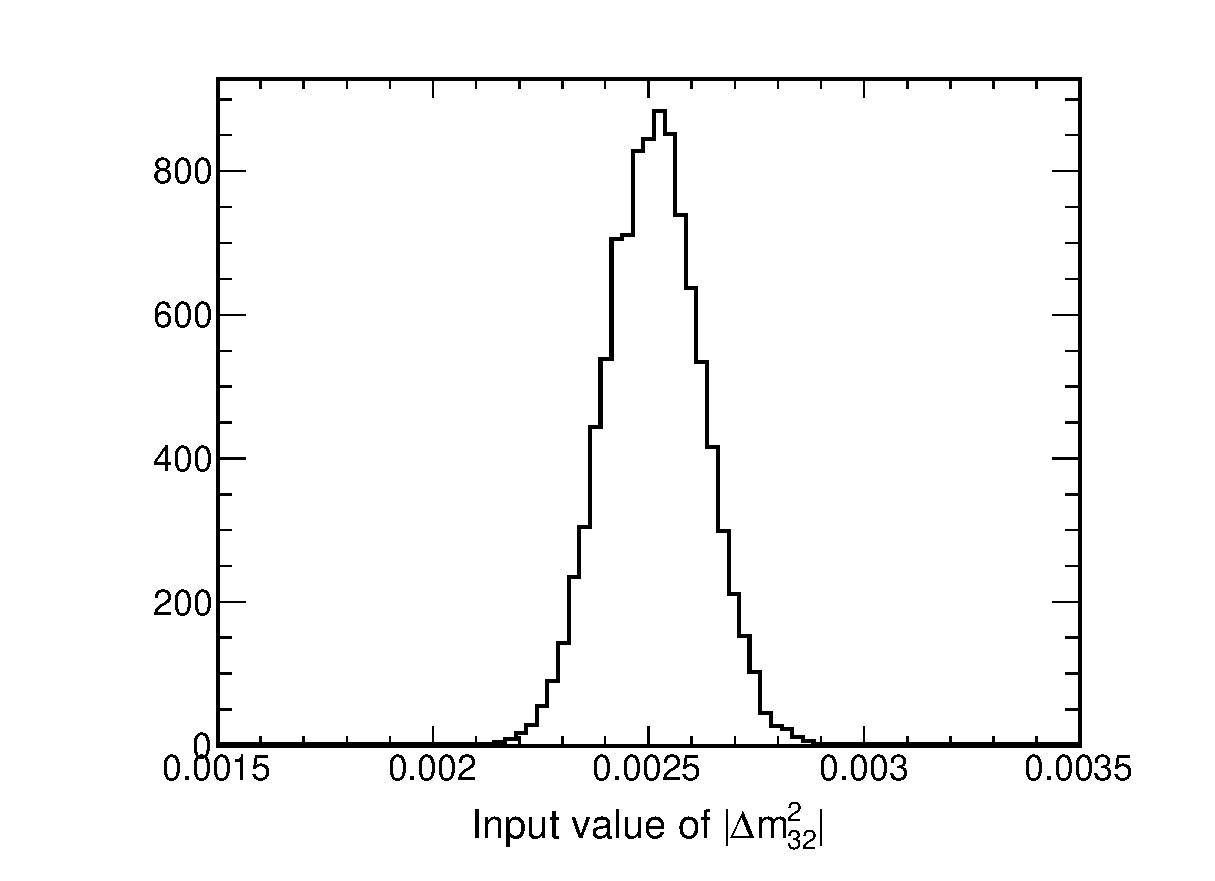
\includegraphics[width=30pc]{./images/fc_surface/input_dm32sq_for_mixing23_0point55}
    \caption {
     True input values of $|\Delta m_{32}^{2}|$ to the toy Monte Carlo experiments used to find the 1D critical value of $\Delta \chi^{2}$ 
     for $\sin^{2}\theta_{23}$ = 0.55. The normal mass hierarchy is assumed.
    }
    \label{fig:input_dm32sq_1DFC}
  \end{minipage}
  \vfill
  \begin{minipage}[t]{0.96\linewidth}
    \center
    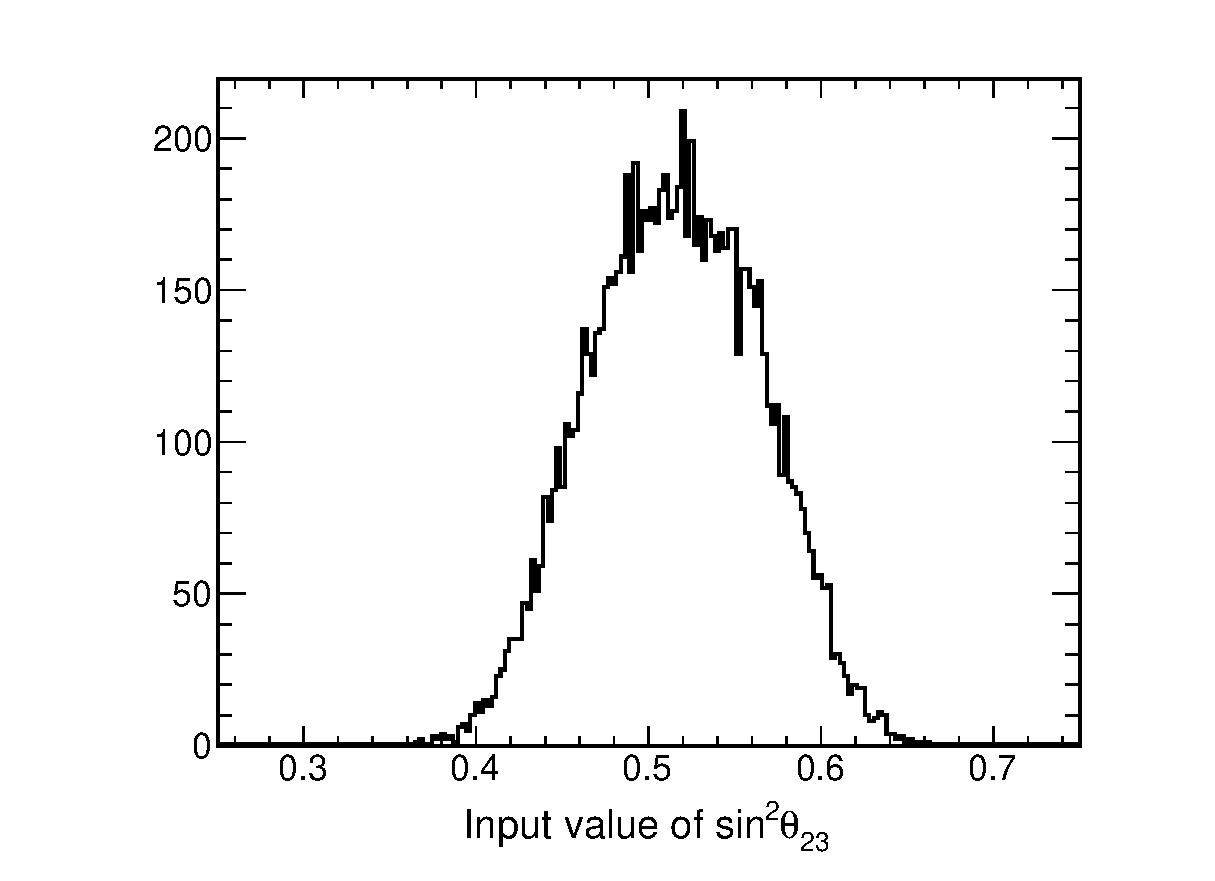
\includegraphics[width=30pc]{./images/fc_surface/input_mixing23_for_dm32sq_2point9Eminus3}
    \caption {
     True input values of $\sin^{2}\theta_{23}$ to the toy Monte Carlo experiments used to find the 1D critical value of $\Delta \chi^{2}$
     for $|\Delta m_{32}^{2}|$ = 2.9$\times$10$^{-3}$ eV$^{2}$/c$^{4}$. The normal mass hierarchy is assumed.
    }
    \label{fig:input_mixing23_1DFC}
  \end{minipage}
\end{figure*}

\clearpage

\section {Validation of the {\em VALOR} Run 1+2+3+4  $\nu_{\mu}$-disappearance analysis}
\label{sec:validation}

The performance of the fitter was evaluated using ensembles of 5k toy MC experiments, and these were
generated with statistical fluctuations and variations of all 41 systematic parameters and the oscillation parameters 
$\sin^{2}\theta_{12}$, $\sin^{2}\theta_{13}$, $\Delta m^{2}_{21}$ and $\delta_{CP}$. Ensembles of experiments were 
generated for different true input values of $\sin^{2}\theta_{23}$ and $|\Delta m^{2}_{32}|$, and for both 
6.5700$\times$10$^{20}$ POT (Run 1+2+3+4) and 7.8$\times$10$^{21}$ POT (the ultimate T2K goal)
These toy MC experiments were fitted using MINUIT and the MINUIT HESSE errors\footnote
{MINOS errors were computed for the SK energy scale systematic because the number of events in a bin is not a smooth 
function of $f^{SK}_{E;r}$. Tweaking this systematic involves migrating events to and from neighbouring bins, and, 
although the number of events itself is a continuous function of $f^{SK}_{E;r}$, there is a discontinuity in the differential 
when moving from positive to negative values of $f^{SK}_{E;r}$. There is also a discontinuity at large values of $f^{SK}_{E;r}$ 
since events are also migrated to and from the next-to-neighbouring bins. For these reasons, HESSE has a problem evaluating 
errors for this systematic parameter.
} 
were computed.

Distributions of fitter residuals for $\sin^{2}\theta_{23}$ and $|\Delta m^{2}_{32}|$ are shown in
Figs.\ \ref{fig:residuals:oscparam:0.370} and \ref{fig:residuals:oscparam:0.650}
for true input values $\sin^{2}\theta_{23}$ = 0.370 and $|\Delta m^{2}_{32}|$ = 2.4$\times$10$^{-3}$ eV$^{2}$/c$^{4}$
and $\sin^{2}\theta_{23}$ = 0.650 and $|\Delta m^{2}_{32}|$ = 2.4$\times$10$^{-3}$ eV$^{2}$/c$^{4}$
respectively, for both 6.5700$\times$10$^{20}$ POT and 7.8$\times$10$^{21}$ POT. A clear three-peak structure is seen 
at Run 1+2+3+4 POT in the distribution of residuals of $\sin^{2}\theta_{23}$, with peaks occurring at
the input value, the mirror of the input value in the other octant, and the maximum disappearance value. 
The peak at the mirror value in the other octant occurs because P($\nu_{\mu} \rightarrow \nu_{\mu}$) is almost identical 
for the input and mirror values (note that the centre of symmetry of $\sin^{2}\theta_{23}$ is at 
$\approx \frac{1}{2(1-\sin^{2}(\theta_{13}))}$ = 0.513 for $\sin^{2}\theta_{13}$ = 0.0251 for reasons given in Appendix E in 
\cite{OurRun123JointOscillationAnalysis}). 
%\footnote{
%  In the 3-flavour oscillation formula\footnotemark
%  $\:P(\nu_{\mu}\rightarrow\nu_{\mu})
%  \approx 1 - \left( \cos^4(\theta_{13})\sin^{2}(2\theta_{23}) + \sin^{2}(\theta_{23})\sin^{2}(2\theta_{13}) \right) \sin^{2}\left(\frac{\Delta m_{31}^{2} L}{4E}\right)$,
%  the maximum amount of disappearance occurs not at $\sin^{2}(\theta_{23}) = 0.5$, but it is offset slightly due to the next-to-leading order term.
%  The extremum occurs at $\sin^{2}(\theta_{23})= \frac{1}{2(1-\sin^{2}(\theta_{13}))} \approx 0.513$.
%  In addition, the oscillation probability is approximately symmetric about this point, meaning that for every input value $!= 0.513$, there exists
%  a mirror point with a similar oscillation probability.
%  More discussion of this effect can be found in Appendix E of \cite{OurRun123JointOscillationAnalysis}.
%}\footnotetext{In the fits, we use full 3-flavour oscillation formulae, and not this approximation.
%  See and Appendix A in \cite{OurRun123DisappAnalysis3Flavour} for full details.}.
The peak at maximal disappearance (which is also at $\sin^{2}\theta_{23}$ $\approx$
0.513) is due to downward statistical fluctuations in the numbers of events in the bins around the oscillation maximum in some
of the toy datasets. When these datasets are fitted, the best fit of $\sin^{2}\theta_{23}$ is the value giving the maximum
physically-allowed disappearance, i.e.\ 0.513. This peak is not seen for 7.8$\times$10$^{21}$ POT since downward statistical 
fluctuations have a smaller effect on the toy datasets at higher statistics. 

Distributions of fitter residuals for $\sin^{2}\theta_{23}$ and $|\Delta m^{2}_{32}|$ are shown in
Fig.\ \ref{fig:residuals:oscparam:0.513}
for true input values $\sin^{2}\theta_{23}$ = 0.513 and $|\Delta m^{2}_{32}|$ = 2.4$\times$10$^{-3}$ eV$^{2}$/c$^{4}$
at 6.5700$\times$10$^{20}$ POT and 7.8$\times$10$^{21}$ POT.
The distribution for $\sin^{2}\theta_{23}$ has a large peak at 0.513 as expected, but also two smaller peaks with one peak in each octant. 
This can be explained by considering the effects of statistical fluctuations in the bins near the oscillation maximum in the toy datasets. 
If there are no statistical fluctuations in these bins, the fitted value of $\sin^{2}\theta_{23}$ is the same as the input value of 0.513, and 
downward statistical fluctuations also result in a fitted value of 0.513. However upward statistical fluctuations in these bins in some datasets mean 
that $\nu_{\mu}$-disappearance is less than maximal, and this results in a fitted value of $\sin^{2}\theta_{23}$ that is different 
from the input value of 0.513. 
The non-maximal values of $\sin^{2}\theta_{23}$ returned by the fitter can be quantified by considering the ratio of the number of events 
in a single bin at the lowest part of the oscillation dip with oscillations to that without oscillations. Examples of this ratio are shown 
in Tab.\ \ref{tab:residuals:3peaks} for 6.5700$\times$10$^{20}$ POT (run 1+2+3+4) and 7.8$\times$10$^{21}$ POT (the ultimate T2K goal). 
As shown in the table, the ratio is 2.672 / 37.93 = 0.070 at 6.5700$\times$10$^{20}$ POT for a dataset without statistical fluctuations. 
The smallest upward statistical fluctuation that can be made is to 3 events, and this increases the ratio to 0.079; this is the ratio that 
would be obtained in a dataset made with an input value of $\sin^{2}\theta_{23}$ of 0.463 (first octant) or 0.565 (second octant). These 
input values are close to the values of the non-maximal peaks in the fitted values of $\sin^{2}\theta_{23}$ as shown by the Gaussian fits in 
Fig.\ \ref{fig:residuals:3peaks}. At 7.8$\times$10$^{21}$ POT, it is necessary to consider upward statistical fluctuations from 31.545 to 
32, 33 and 34 events in order to obtain a ratio of number of events with oscillations to that without oscillations corresponding to the values 
of the non-maximal peaks in the fitted values of $\sin^{2}\theta_{23}$. 
%Such upward fluctuations are to be expected as shown by the 
%distribution of 100k Poisson fluctuations from a mean of 31.545 in the right plot in Fig.\ \ref{fig:residuals:poisson_fluct}.


%The two extra peaks appear at one specific value and its mirror point,
%and this value changes with increasing POT.
%The effect can be seen more clearly in Fig.\ \ref{fig:residuals:3peaks}.
%The values where the extra peaks appear can be explained in terms of statistical fluctuations
%at the oscillation dip. If an upward fluctuation\footnote{
%  The same explanation works also for a downward fluctuations adding a normalization factor.}
%is applied to the number of events at the oscillation dip, the ratio between number of events at
%the oscillation dip with respect to the case of no oscillations varies. The fitter then returns as
%best-fit value for $\sin^{2}\theta_{23}$  a value matching the ratio at the oscillation dip of the fluctuated spectrum.
%Simply observing this ratio at different values of $\sin^{2}\theta_{23}$ presented in Fig.\ \ref{fig:residuals:ratio_at_minimum}
%the value of $\sin^{2}\theta_{23}$ giving the same ratio as the fluctuated spectrum can be found.
%At current POT an upward fluctuation of a single event (+1) explains the value of the extra peaks
%in Fig.\ \ref{fig:residuals:3peaks}, but for higher POT it is necessary to consider upward fluctuations
%of more than one event (+1,+2,+3..). This is because at higher POT the number of events at the
%oscillation dip before fluctuations is larger, and therefore it is more probable that a larger
%fluctuation can occur. This is shown in Fig.\ \ref{fig:residuals:poisson_fluct} where 100k Poissonian fluctuations
%of the number of events at the oscillation dip for current POT (left plot) and ultimate POT goal (right plot) were thrown.
%Tab.\ \ref{tab:residuals:3peaks} presents a summary of this explanation, where the number of events
%at the oscillation dip and the ratio with respect to no oscillations are presented for a true input value
%$\sin^{2}\theta_{23}$ = 0.513 at current and the ultimate POT goal and different fluctuations.
%The table also contains the values of $\sin^{2}\theta_{23}$ from Fig.\ \ref{fig:residuals:ratio_at_minimum}
%matching the ratio of number of events at the oscillation dip with respect to no oscillations.
%Those values are to be compared with the values of $\sin^{2}\theta_{23}$ found for the extra peaks
%in Fig.\ \ref{fig:residuals:3peaks} and presented in the last two columns. 
% The probability for each fluctuation to occur, computed as the fraction of times
% appearing in \ref{fig:residuals:poisson_fluct} divided by the total, is also included in this table.
%There are multiple effects contributing to the spread of the extra peaks 
%including systematic fluctuations changing $N_{exp}$ from which $N_{obs}$ is drawn,
%that there are multiple bins in the oscillation dip region for which this effect will be important,
%and rarer large statistical fluctuations.

% Residual distributions for the systematic parameters are shown in
% Figs.\ \ref{fig:syst_residuals1:run1234:0.370}-\ref{fig:syst_residuals4:run1234:0.370} for
% $\sin^{2}\theta_{23}$ = 0.370 and $|\Delta m^{2}_{32}|$ = 2.4$\times$10$^{-3}$ eV$^{2}$/c$^{4}$,
% Figs.\ \ref{fig:syst_residuals1:run1234:0.513}-\ref{fig:syst_residuals4:run1234:0.513} for
% $\sin^{2}\theta_{23}$ = 0.513 and $|\Delta m^{2}_{32}|$ = 2.4$\times$10$^{-3}$ eV$^{2}$/c$^{4}$,
% and
% Figs.\ \ref{fig:syst_residuals1:run1234:0.650}-\ref{fig:syst_residuals4:run1234:0.650} for
% $\sin^{2}\theta_{23}$ = 0.650 and $|\Delta m^{2}_{32}|$ = 2.4$\times$10$^{-3}$ eV$^{2}$/c$^{4}$.
% The corresponding pull plots are shown in
% Figs.\ \ref{fig:syst_pulls1:run1234:0.370}-\ref{fig:syst_pulls4:run1234:0.370},
% Figs.\ \ref{fig:syst_pulls1:run1234:0.513}-\ref{fig:syst_pulls4:run1234:0.513}, and
% Figs.\ \ref{fig:syst_pulls1:run1234:0.650}-\ref{fig:syst_pulls4:run1234:0.650}.

% % replace this paragraph with the above if we're showing the residual plots
% Pull distributions for the systematic parameters are shown in
% Figs.\ \ref{fig:syst_pulls1:run1234:0.370}-\ref{fig:syst_pulls4:run1234:0.370} for
% $\sin^{2}\theta_{23}$ = 0.370 and $|\Delta m^{2}_{32}|$ = 2.4$\times$10$^{-3}$ eV$^{2}$/c$^{4}$,
% Figs.\ \ref{fig:syst_pulls1:run1234:0.513}-\ref{fig:syst_pulls4:run1234:0.513} for
% $\sin^{2}\theta_{23}$ = 0.513 and $|\Delta m^{2}_{32}|$ = 2.4$\times$10$^{-3}$ eV$^{2}$/c$^{4}$,
% and
% Figs.\ \ref{fig:syst_pulls1:run1234:0.650}-\ref{fig:syst_pulls4:run1234:0.650} for
% $\sin^{2}\theta_{23}$ = 0.650 and $|\Delta m^{2}_{32}|$ = 2.4$\times$10$^{-3}$ eV$^{2}$/c$^{4}$.

Distributions of pulls of the 41 systematic parameters and four non-23 oscillation parameters are shown in Figs.\
\ref{fig:pulls:syst:0.370}, \ref{fig:pulls:syst:0.650} and \ref{fig:pulls:syst:0.513},
for true input values of 
$\sin^{2}\theta_{23}$ = 0.370 and $|\Delta m^{2}_{32}|$ = 2.4$\times$10$^{-3}$ eV$^{2}$/c$^{4}$,
$\sin^{2}\theta_{23}$ = 0.650 and $|\Delta m^{2}_{32}|$ = 2.4$\times$10$^{-3}$ eV$^{2}$/c$^{4}$, and
$\sin^{2}\theta_{23}$ = 0.513 and $|\Delta m^{2}_{32}|$ = 2.4$\times$10$^{-3}$ eV$^{2}$/c$^{4}$ respectively.
In these figures, the pulls are calculated as $(f_{bestfit} - f_{true}) / \sigma_{fit}$. 
For most systematics, the distributions are approximately Gaussian with
mean 0, width 1.

A summary of the pull mean, RMS, skewness, and kurtosis
is shown in Figs.\
\ref{fig:pulls:syst:summary:0.370}, \ref{fig:pulls:syst:summary:0.650} and \ref{fig:pulls:syst:summary:0.513},
for input values of 
$\sin^{2}\theta_{23}$ = 0.370 and $|\Delta m^{2}_{32}|$ = 2.4$\times$10$^{-3}$ eV$^{2}$/c$^{4}$,
$\sin^{2}\theta_{23}$ = 0.650 and $|\Delta m^{2}_{32}|$ = 2.4$\times$10$^{-3}$ eV$^{2}$/c$^{4}$, and
$\sin^{2}\theta_{23}$ = 0.513 and $|\Delta m^{2}_{32}|$ = 2.4$\times$10$^{-3}$ eV$^{2}$/c$^{4}$ respectively.
Most systematic distributions are Gaussian, with mean $\approx0$, RMS $\approx1$, skewness $\approx0$ and kurtosis $\approx0$.
%The kurtosis has some spread, due to peaks forming from the limited statistics of the study.
%The KS test also suffers from limited statistics.
%Individual pull plots can be found in Appendix\ \ref{apdx:validiation}.

No problems were identified with the fitter, which performed as expected.
There are some small biases in the pull distributions for some systematic parameters, but these biases are understood:
\begin{itemize}
\item {\bf \boldmath$\delta_{CP}$.}
  This systematic is thrown uniformly between $-\pi$ and $+\pi$ (rather than with a Gaussian distribution),
  is constrained between $-\pi$ and $+\pi$ in the fit,
  and has no penalty term. Therefore a Gaussian distribution is not expected.
\item {\bf Spectral function.}
  This systematic is limited to the range [0,1], both for toy experiment generation,
  and in the fit.
  It is constrained with a Gaussian constraint.
  Therefore a Gaussian distribution with mean 0, width 1 is not expected.
\item {\bf $\pi$-less $\Delta$ decay.}
  The bias is due to the method of calculation of event 
  weights when this parameter is varied. By default, 20\% of $\Delta$s decay in this way in NEUT, and the uncertainty 
  is 20\%. This means that it is unphysical to tweak this parameter to be more negative than -1$\sigma$, and 
  consequently there is an asymmetry in weights between positive tweaks (which change continuously as the tweak 
  increases) and negative tweaks (for which all tweaks more negative than -1$\sigma$ are assigned the same weight 
  as that for a -1$\sigma$ tweak).
  This leads to a small negative bias.
\item {\bf SuperK energy scale.}
  %For negative tweaks of this parameter, the nominally-empty bin 0.20-0.25 GeV becomes filled with events
  %(0.25(0.52), for a -1(-2)$\sigma$ tweak).
  % 0.25259 events in the 0.20-0.25 GeV bin at -1 sigma
  % (1*ln(1/0.25259)) + 0.25259 - 1 = 0.628
  % 0.51791 events in the 0.20-0.25 GeV bin at -2 sigma
  % (1*ln(1/0.51791)) + 0.51791 - 1 = 0.1758
  %From Eqn.\ \ref{eq:chisquare}
  %the $\chi^2$ contribution in this bin, for a -1(-2)$\sigma$ tweak is 0.25(0.52) at $N_{obs} = 0$, and 0.63(0.18) at $N_{obs} = 1$.
  %This means for toy experiments created with a largely negative value of $f_{E; r}^{SK}$, that has a statistical fluctuation
  %such that $N_{obs} = 0$ in that bin, fits returning less than the true value of $f_{E; r}^{SK}$ are disfavoured.
  %This leads to a small positive bias in the pull.
  This systematic is different from the others in that it migrates events from bin to bin instead of increasing or decreasing the 
  numbers of events in the bins of reconstructed energy. Its pull is not expected to be a Gaussian with zero mean since the shape 
  of the predicted 1 $\mu$-like ring energy spectrum is not symmetric, and, consequently, a positive tweak of this parameter has a 
  different effect on that spectrum from a negative tweak (please see figure 46 in the supplement to this technical note). 
  %When fitting  the toy datasets, this parameter would be expected to be moved up from zero if there is an upward statistical fluctuation 
  %below the oscillation maximum and a downward one above it. The fitter would move this parameter down from zero if there is a ‪downward
  %statistical fluctuation below the oscillation maximum and an upward one above it. ‬When Poisson fluctuations are made of a small number
  %of events in a bin of the reconstructed energy distribution, a downward fluctuation is more likely than an upward fluctuation. For example, a 
  %Poisson distribution with mean 3 has P(1) = 0.149 and P(2) = 0.224, whereas P(4) = 0.168 and P(5) = 0.101. The bins immediately below the 
  %oscillation maximum have fewer events than those immediately above it, and a downward fluctuation is slightly more likely in the bins 
  %below the maximum than those above it. This explains the small positive bias in the pull of this parameter. 
\item {\bf NC SuperK detector efficiency + FSI + SI.} 
  The bias comes from the low statistics at current POT.
  When Poisson fluctuations are made of the bin contents of the $E_{reco}$ distributions, a downward fluctuation is more likely than an upward
  fluctuation. For example, a Poisson distribution with mean 3 has P(1) = 0.149 and P(2) = 0.224, whereas P(4) = 0.168 and P(5) = 0.101. The 
  NC events are mainly around the oscillation maximum where there are few events, and downward Poisson fluctuations are more likely than upward 
  ones. Fitting these downward fluctuations involves moving this parameter down from zero, and this explains the negative bias in its pull. 
  When moving away from the point of maximal disappearance as input
  (and so reducing the depth of the oscillation dip),
  the NC bin in the SuperK detector efficiency + FSI + SI matrix bias is reduced.
\end{itemize}
The pull distributions for these 5 systematics are shown in Figs.\ 
\ref{fig:pulls:syst:important:0.370}, \ref{fig:pulls:syst:important:0.650} and \ref{fig:pulls:syst:important:0.513},
for input values of 
$\sin^{2}\theta_{23}$ = 0.370 and $|\Delta m^{2}_{32}|$ = 2.4$\times$10$^{-3}$ eV$^{2}$/c$^{4}$,
$\sin^{2}\theta_{23}$ = 0.650 and $|\Delta m^{2}_{32}|$ = 2.4$\times$10$^{-3}$ eV$^{2}$/c$^{4}$, and
$\sin^{2}\theta_{23}$ = 0.513 and $|\Delta m^{2}_{32}|$ = 2.4$\times$10$^{-3}$ eV$^{2}$/c$^{4}$ respectively.


%
% Osc param residuals
% 
\begin{figure*}[htb]
  \center
  \includegraphics[width=32pc]{{./images/fit_bias/residuals_oscparams_0.002400_0.370}.eps}
  \caption {
    Distributions of fitter residuals for $\sin^{2}\theta_{23}$ and $|\Delta m^2_{32}|$ for 5k toy MC experiments,
    generated at $\sin^{2}\theta_{23}$ = 0.370 and
    $|\Delta m^{2}_{32}|$ = 2.4$\times$10$^{-3}$ eV$^{2}$/c$^{4}$,
    including statistical fluctuations and with randomized systematic and non-23 oscillation parameters.
    The distribution is shown for both
    6.5700$\times$10$^{20}$ POT (Run 1+2+3+4, black histogram) and 7.8$\times$10$^{21}$ POT (the T2K ultimate goal, 
    red histogram).
  }
  \label{fig:residuals:oscparam:0.370}
\end{figure*}

\begin{figure*}[htb]
  \center
  \includegraphics[width=32pc]{{./images/fit_bias/residuals_oscparams_0.002400_0.650}.eps}
  \caption {
    Distributions of fitter residuals for $\sin^{2}\theta_{23}$ and $|\Delta m^2_{32}|$ for 5k toy MC experiments,
    generated at $\sin^{2}\theta_{23}$ = 0.650 and
    $|\Delta m^{2}_{32}|$ = 2.4$\times$10$^{-3}$ eV$^{2}$/c$^{4}$,
    including statistical fluctuations and with randomized systematic and non-23 oscillation parameters.
    The distribution is shown for both
    6.5700$\times$10$^{20}$ POT (Run 1+2+3+4, black histogram) and 7.8$\times$10$^{21}$ POT (the T2K ultimate goal, 
    red histogram).
  }
  \label{fig:residuals:oscparam:0.650}
\end{figure*}

\begin{figure*}[htb]
  \center
  \includegraphics[width=32pc]{{./images/fit_bias/residuals_oscparams_0.002400_0.513}.eps}
  \caption {
    Distributions of fitter residuals for $\sin^{2}\theta_{23}$ and $|\Delta m^2_{32}|$ for 5k toy MC experiments,
    generated at $\sin^{2}\theta_{23}$ = 0.513 and
    $|\Delta m^{2}_{32}|$ = 2.4$\times$10$^{-3}$ eV$^{2}$/c$^{4}$,
    including statistical fluctuations and with randomized systematic and non-23 oscillation parameters.
    The distribution is shown for both
    6.5700$\times$10$^{20}$ POT (Run 1+2+3+4, black histogram) and 7.8$\times$10$^{21}$ POT (the T2K ultimate goal, 
    red histogram).
  }
  \label{fig:residuals:oscparam:0.513}
\end{figure*}

\begin{figure*}[htb]
  \center
  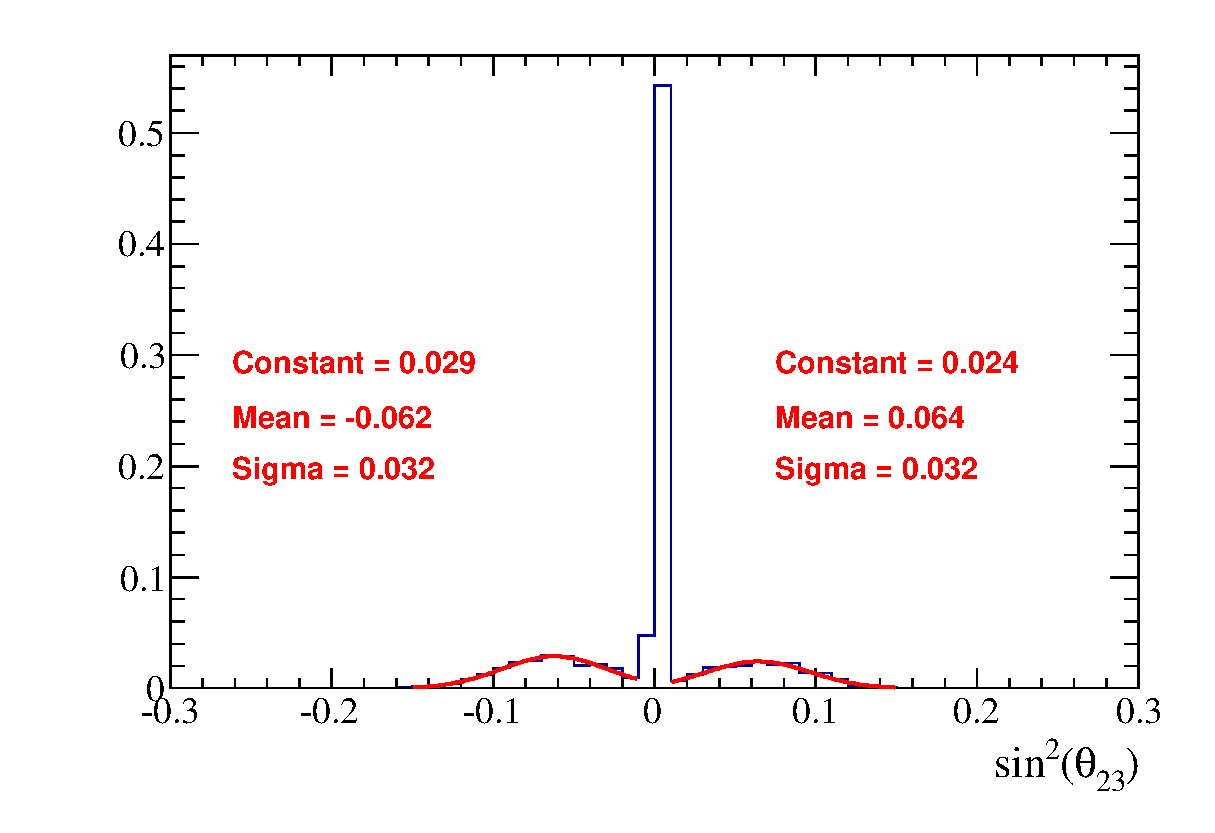
\includegraphics[width=20pc]{./images/fit_bias/Residuals_3peaks.eps}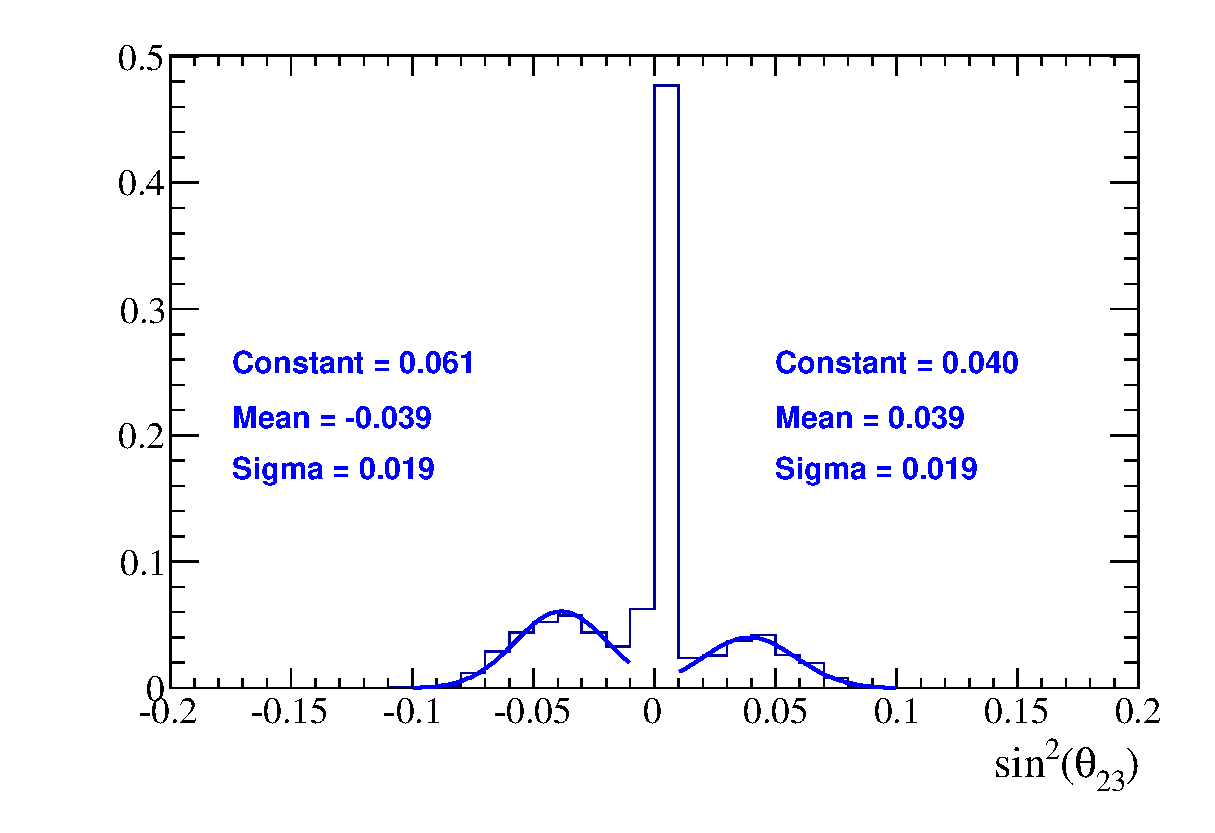
\includegraphics[width=20pc]{./images/fit_bias/Residuals_3peaks_goal.eps}
  \caption {
    Distributions of fitter residuals for $\sin^{2}\theta_{23}$ for 5k toy MC experiments,
    generated at $\sin^{2}\theta_{23}$ = 0.513 and
    $|\Delta m^{2}_{32}|$ = 2.4$\times$10$^{-3}$ eV$^{2}$/c$^{4}$,
    including statistical fluctuations and with randomized systematic and non-23 oscillation parameters,
    stressing the three-peak structure and including a Gaussian fit for the extra peaks at non-maximal disappearance.
    The distribution is shown for both
    6.5700$\times$10$^{20}$ POT (Run 1+2+3+4, left plot) and 7.8$\times$10$^{21}$ POT (the T2K ultimate goal, right plot).
  }
  \label{fig:residuals:3peaks}
\end{figure*}

\begin{table}[htbp]
\center
\begin{tabular}{|p{1.5cm}|p{2.5cm}|p{1.5cm}|p{1cm}|p{1.6cm}|p{1.6cm}|p{1.6cm}|p{1.6cm}|}
\hline
POT &   & Number  & Ratio &  \multicolumn{2}{c|}{Input value of $\sin^{2}\theta_{23}$} & \multicolumn{2}{c|}{Peak of} \\
& & of events & osc/        & \multicolumn{2}{c|}{giving this ratio}   & \multicolumn{2}{c|}{non-maximal fitted} \\
  & &  & no osc        &   \multicolumn{2}{c|}{osc/no osc}  & \multicolumn{2}{c|}{values of $\sin^{2}\theta_{23}$} \\
\cline{5-8}
   & &  &         & (Octant 1) & (Octant 2) & (Octant 1) & (Octant 2) \\
\hline \hline
\multirow{3}{*}{6.57$\times$10$^{20}$} & No oscillations  & 37.934 & 1 & & & \multirow{3}{*}{0.451} & \multirow{3}{*}{0.577} \\
\cline{2-6}
 & $\sin^{2}\theta_{23}$ = 0.513 (no fluctuation) & 2.672 & 0.070 & & & & \\
\cline{2-6}
 & $\sin^{2}\theta_{23}$ = 0.513 (fluctuation 1) & 3 & 0.079 & 0.463 & 0.565 & & \\
\hline \hline
\multirow{7}{*}{7.8$\times$10$^{21}$} & No oscillations & 450.352 & 1 & & & \multirow{7}{*}{0.474} & \multirow{7}{*}{0.552} \\
\cline{2-6}
 & $\sin^{2}\theta_{23}$ = 0.513 (no fluctuation) & 31.545 & 0.070 & & & & \\
\cline{2-6}
 & $\sin^{2}\theta_{23}$ = 0.513 (fluctuation 1)  & 32 & 0.071 & 0.497 & 0.531 &  &  \\
\cline{2-6}
 & $\sin^{2}\theta_{23}$ = 0.513 (fluctuation 2)  & 33 & 0.073 & 0.484 & 0.544 &  &  \\
\cline{2-6}
 &$\sin^{2}\theta_{23}$ = 0.513 (fluctuation 3) & 34 & 0.075 & 0.474 & 0.553 &  &  \\
\cline{2-6}
 &$\sin^{2}\theta_{23}$ = 0.513 (fluctuation 4) & 35 & 0.078 & 0.467 & 0.561 &  & \\
\cline{2-6}
 &$\sin^{2}\theta_{23}$ = 0.513 (fluctuation 5) & 36 & 0.080 & 0.461 & 0.566 &  & \\
\hline
\end{tabular}
\caption{
Numbers of events in a single bin at the lowest part of the oscillation dip with oscillations and ratio to number without oscillations for a true input 
value $\sin^{2}\theta_{23}$ = 0.513 at 6.57$\times$10$^{20}$ POT (Run 1+2+3+4) and 7.8$\times$10$^{21}$ POT (the ultimate T2K goal). These numbers are 
shown without statistical fluctuations and with different upward fluctuations. Also shown are the input values of $\sin^{2}\theta_{23}$ to toy datasets 
from Fig.\ \ref{fig:residuals:ratio_at_minimum} matching the ratio of number of events with oscillations to number without oscillations. These values of 
$\sin^{2}\theta_{23}$ can be compared with the peaks of the non-maximal fitted values of $\sin^{2}\theta_{23}$ from the Gaussian fits in Fig.\ 
\ref{fig:residuals:3peaks}.}
\label{tab:residuals:3peaks}
\end{table}

\begin{figure*}[htb]
  \center
  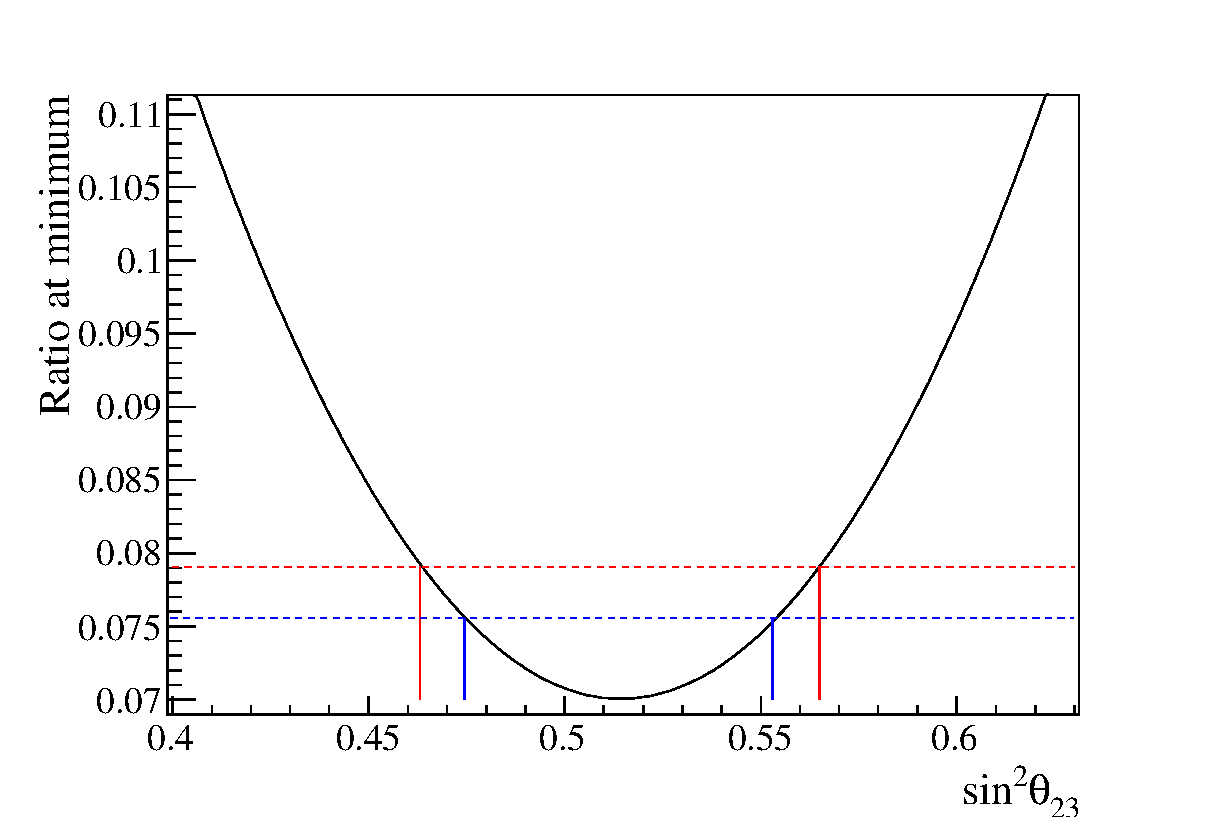
\includegraphics[width=25pc]{./images/fit_bias/Ratio_at_minimum.eps}
  \caption {
    Ratio of number of events in a single bin at the lowest part of the oscillation dip for toy datasets
    created with different input values of $\sin^{2}\theta_{23}$ to number without oscillations
    against the input value of $\sin^{2}\theta_{23}$. Red (blue) lines show the value corresponding to
    the ratio found at 6.5700$\times$10$^{20}$ POT (7.8$\times$10$^{21}$ POT, the T2K ultimate POT goal)
    in Fig.\ \ref{fig:residuals:3peaks}.
  }
  \label{fig:residuals:ratio_at_minimum}
\end{figure*}


%\begin{figure*}[htb]
%  \center
%  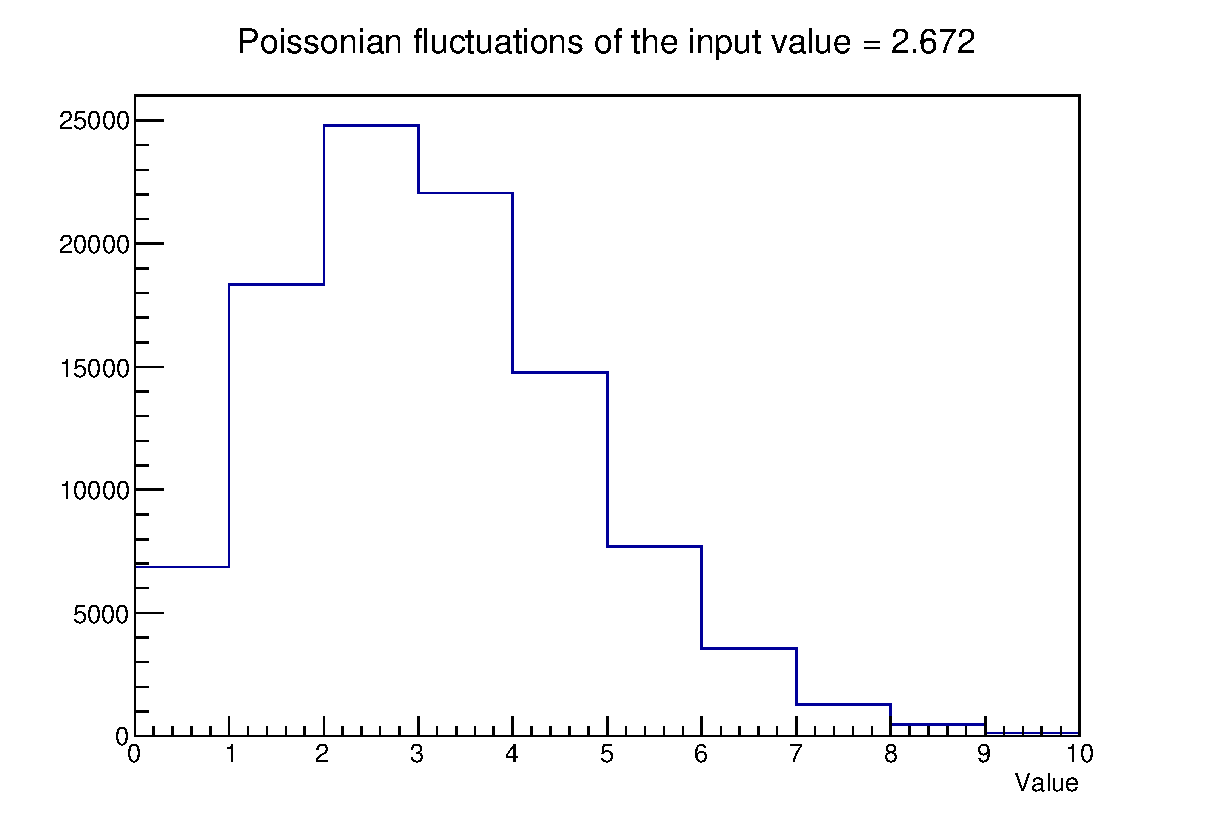
\includegraphics[width=20pc]{./images/fit_bias/Poisson_fluct_dip.eps}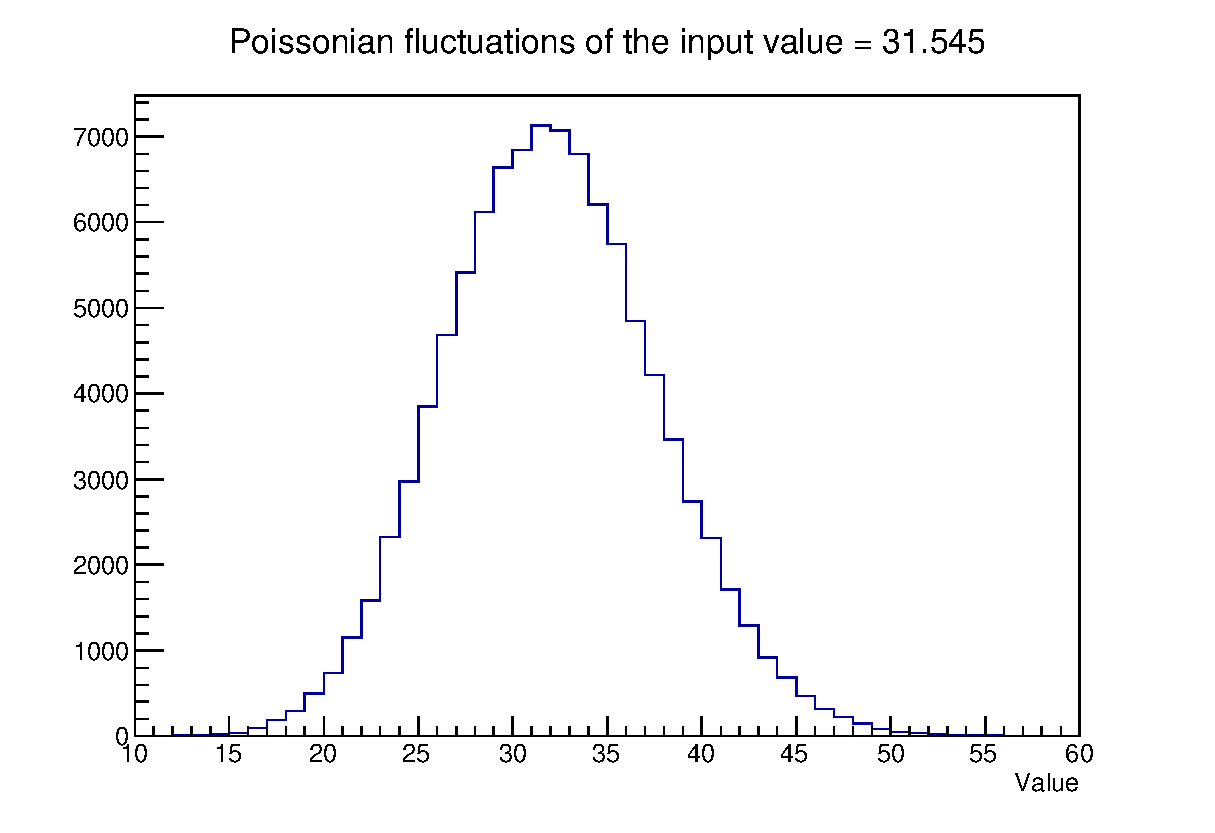
\includegraphics[width=20pc]{./images/fit_bias/Poisson_fluct_dip_goal.eps}
%  \caption {
%    Distributions of 100k Poisson fluctuations of the number of
%    events in a single bin at the lowest part of the oscillation dip for an input value of $\sin^{2}\theta_{23}$ = 0.513
%    These distributions are shown for means of 2.672 events (for 6.5700$\times$10$^{20}$ POT, left plot) and 31.545 events
%    (for 7.8$\times$10$^{21}$ POT, the T2K ultimate POT goal, right plot).
%  }
%  \label{fig:residuals:poisson_fluct}
%\end{figure*}



%
% Systematic pull & summary plots
%
\begin{figure*}[htb]
  \center
  \includegraphics[width=40pc]{{./images/fit_bias/nuis_sys_0.002400_0.370_allpulls}.eps}
  \caption {
    Systematic pull distributions for all systematic parameters for
    5k toy MC experiments at 6.5700$\times$10$^{20}$ POT 
    generated at $\sin^{2}\theta_{23}$ = 0.370 and
    $|\Delta m^{2}_{32}|$ = 2.4$\times$10$^{-3}$ eV$^{2}$/c$^{4}$,
    including statistical fluctuations and with randomized systematic parameters.
    A Gaussian distribution of mean 0, width 1 is shown for reference.
    The two parameters that do not have a Gaussian distribution are $\delta_{CP}$ and $f_{SF; t, r}$.
  }
  \label{fig:pulls:syst:0.370}
\end{figure*}

\begin{figure*}[htb]
  \center
  \includegraphics[width=50pc,angle=270]{{./images/fit_bias/nuis_sys_0.002400_0.370_bigsummary}.eps}
  \caption {
    Summary of systematic pull distributions for all systematic parameters for
    5k toy MC experiments at 6.5700$\times$10$^{20}$ POT 
    generated at $\sin^{2}\theta_{23}$ = 0.370 and
    $|\Delta m^{2}_{32}|$ = 2.4$\times$10$^{-3}$ eV$^{2}$/c$^{4}$,
    including statistical fluctuations and with randomized systematic parameters.
    The tests shown are the mean, RMS, skewness and kurtosis.
    % and the p-value from 
    % a Kolmogorov-Smirnov test comparing the pull distribution with a normal distribution of
    % mean 0, width 1.
  }
  \label{fig:pulls:syst:summary:0.370}
\end{figure*}

\begin{figure*}[htb]
  \center
  \includegraphics[width=38pc]{{./images/fit_bias/nuis_sys_0.002400_0.370_importpull_1_5}.eps}
  \caption {
    Pull distributions for $\delta_{CP}$,
    $f_{SF; t, r}$,
    $f_{\pi-less\Delta; t, r}$,
    $f_{E; r}^{SK}$,
    and $f_{i; r}^{SK+FSI}$,
    computed from fits of 5k toy MC experiments at 
    6.5700$\times$10$^{20}$ POT, generated at $\sin^{2}\theta_{23}$ = 0.370 and
    $|\Delta m^{2}_{32}|$ = 2.4$\times$10$^{-3}$ eV$^{2}$/c$^{4}$,
    including statistical fluctuations and with randomized systematic parameters.
  }
  \label{fig:pulls:syst:important:0.370}
\end{figure*}

\begin{figure*}[htb]
  \center
  \includegraphics[width=40pc]{{./images/fit_bias/nuis_sys_0.002400_0.650_allpulls}.eps}
  \caption {
    Systematic pull distributions for all systematic parameters for
    5k toy MC experiments at 6.5700$\times$10$^{20}$ POT 
    generated at $\sin^{2}\theta_{23}$ = 0.650 and
    $|\Delta m^{2}_{32}|$ = 2.4$\times$10$^{-3}$ eV$^{2}$/c$^{4}$,
    including statistical fluctuations and with randomized systematic parameters.
    A Gaussian distribution of mean 0, width 1 is shown for reference.
    The two non-Gaussian parameters are $\delta_{CP}$ and $f_{SF; t, r}$.
  }
  \label{fig:pulls:syst:0.650}
\end{figure*}

\begin{figure*}[htb]
  \center
  \includegraphics[width=50pc,angle=270]{{./images/fit_bias/nuis_sys_0.002400_0.650_bigsummary}.eps}
  \caption {
    Summary of systematic pull distributions for all systematic parameters for
    5k toy MC experiments at 6.5700$\times$10$^{20}$ POT 
    generated at $\sin^{2}\theta_{23}$ = 0.650 and
    $|\Delta m^{2}_{32}|$ = 2.4$\times$10$^{-3}$ eV$^{2}$/c$^{4}$,
    including statistical fluctuations and with randomized systematic parameters.
    The tests shown are the mean, RMS, skewness and kurtosis.
    % and the p-value from 
    % a Kolmogorov-Smirnov test comparing the pull distribution with a normal distribution of
    % mean 0, width 1.
  }
  \label{fig:pulls:syst:summary:0.650}
\end{figure*}

\begin{figure*}[htb]
  \center
  \includegraphics[width=38pc]{{./images/fit_bias/nuis_sys_0.002400_0.650_importpull_1_5}.eps}
  \caption {
    Pull distributions for $\delta_{CP}$,
    $f_{SF; t, r}$,
    $f_{\pi-less\Delta; t, r}$,
    $f_{E; r}^{SK}$,
    and $f_{i; r}^{SK+FSI}$,
    computed from fits of 5k toy MC experiments at 
    6.5700$\times$10$^{20}$ POT, generated at $\sin^{2}\theta_{23}$ = 0.650 and
    $|\Delta m^{2}_{32}|$ = 2.4$\times$10$^{-3}$ eV$^{2}$/c$^{4}$,
    including statistical fluctuations and with randomized systematic parameters.
  }
  \label{fig:pulls:syst:important:0.650}
\end{figure*}

\begin{figure*}[htb]
  \center
  \includegraphics[width=40pc]{{./images/fit_bias/nuis_sys_0.002400_0.513_allpulls}.eps}
  \caption {
    Systematic pull distributions for all systematic parameters for
    5k toy MC experiments at 6.5700$\times$10$^{20}$ POT 
    generated at $\sin^{2}\theta_{23}$ = 0.513 and
    $|\Delta m^{2}_{32}|$ = 2.4$\times$10$^{-3}$ eV$^{2}$/c$^{4}$,
    including statistical fluctuations and with randomized systematic parameters.
    A Gaussian distribution of mean 0, width 1 is shown for reference.
    The two non-Gaussian parameters are $\delta_{CP}$ and $f_{SF; t, r}$.
  }
  \label{fig:pulls:syst:0.513}
\end{figure*}

\begin{figure*}[htb]
  \center
  \includegraphics[width=50pc,angle=270]{{./images/fit_bias/nuis_sys_0.002400_0.513_bigsummary}.eps}
  \caption {
    Summary of systematic pull distributions for all systematic parameters for
    5k toy MC experiments at 6.5700$\times$10$^{20}$ POT 
    generated at $\sin^{2}\theta_{23}$ = 0.513 and
    $|\Delta m^{2}_{32}|$ = 2.4$\times$10$^{-3}$ eV$^{2}$/c$^{4}$,
    including statistical fluctuations and with randomized systematic parameters.
    The tests shown are the mean, RMS, skewness and kurtosis.
    % and the p-value from 
    % a Kolmogorov-Smirnov test comparing the pull distribution with a normal distribution of
    % mean 0, width 1.
  }
  \label{fig:pulls:syst:summary:0.513}
\end{figure*}

\begin{figure*}[htb]
  \center
  \includegraphics[width=38pc]{{./images/fit_bias/nuis_sys_0.002400_0.513_importpull_1_5}.eps}
  \caption {
    Pull distributions for $\delta_{CP}$,
    $f_{SF; t, r}$,
    $f_{\pi-less\Delta; t, r}$,
    $f_{E; r}^{SK}$,
    and $f_{i; r}^{SK+FSI}$,
    computed from fits of 5k toy MC experiments at 
    6.5700$\times$10$^{20}$ POT, generated at $\sin^{2}\theta_{23}$ = 0.513 and
    $|\Delta m^{2}_{32}|$ = 2.4$\times$10$^{-3}$ eV$^{2}$/c$^{4}$,
    including statistical fluctuations and with randomized systematic parameters.
  }
  \label{fig:pulls:syst:important:0.513}
\end{figure*}



% these have been replaced with the same information, just combining
% current & future POT
% %
% % Osc param residuals for 0.37
% %
% \begin{figure*}[htb]
% \begin{minipage}[t]{0.48\linewidth}
% \center
% \includegraphics[width=20pc]{{./images/fit_bias/nuis_sys_0.002400_0.370_residual_0}.eps}
% \caption {
%   Residual distributions for $\sin^{2}\theta_{23}$ and $|\Delta m^2_{32}|$ 5k toy MC experiments at 
%   6.5700$\times$10$^{20}$ POT, generated at $\sin^{2}\theta_{23}$ = 0.370 and
%   $|\Delta m^{2}_{32}|$ = 2.4$\times$10$^{-3}$ eV$^{2}$/c$^{4}$,
%   including statistical fluctuations and with randomized systematic parameters.
% }
% \label{fig:syst_residuals:oscparam:run1234:0.370}
% \end{minipage}
% \hspace{0.06\linewidth}
% \begin{minipage}[t]{0.48\linewidth}
% \center
% \includegraphics[width=20pc]{{./images/fit_bias/nuis_sys_0.002400_0.370_goalpot_residual_0}.eps}
% \caption {
%   Residual distributions for $\sin^{2}\theta_{23}$ and $|\Delta m^2_{32}|$ 5k toy MC experiments at 
%   7.8$\times$10$^{21}$ POT (the T2K ultimate POT goal), generated at $\sin^{2}\theta_{23}$ = 0.370 and
%   $|\Delta m^{2}_{32}|$ = 2.4$\times$10$^{-3}$ eV$^{2}$/c$^{4}$,
%   including statistical fluctuations and with randomized systematic parameters.
% }
% \label{fig:syst_residuals:oscparam:potgoal:0.370}
% \end{minipage}
% \end{figure*}

% %
% % Osc param residuals for 0.65
% %
% \begin{figure*}[htb]
% \begin{minipage}[t]{0.48\linewidth}
% \center
% \includegraphics[width=20pc]{{./images/fit_bias/nuis_sys_0.002400_0.650_residual_0}.eps}
% \caption {
%   Residual distributions for $\sin^{2}\theta_{23}$ and $|\Delta m^2_{32}|$ 5k toy MC experiments at 
%   6.5700$\times$10$^{20}$ POT, generated at $\sin^{2}\theta_{23}$ = 0.650 and
%   $|\Delta m^{2}_{32}|$ = 2.4$\times$10$^{-3}$ eV$^{2}$/c$^{4}$,
%   including statistical fluctuations and with randomized systematic parameters.
% }
% \label{fig:syst_residuals:oscparam:run1234:0.650}
% \end{minipage}
% \hspace{0.06\linewidth}
% \begin{minipage}[t]{0.48\linewidth}
% \center
% \includegraphics[width=20pc]{{./images/fit_bias/nuis_sys_0.002400_0.650_goalpot_residual_0}.eps}
% \caption {
%   Residual distributions for $\sin^{2}\theta_{23}$ and $|\Delta m^2_{32}|$ 5k toy MC experiments at 
%   7.8$\times$10$^{21}$ POT (the T2K ultimate POT goal), generated at $\sin^{2}\theta_{23}$ = 0.650 and
%   $|\Delta m^{2}_{32}|$ = 2.4$\times$10$^{-3}$ eV$^{2}$/c$^{4}$,
%   including statistical fluctuations and with randomized systematic parameters.
% }
% \label{fig:syst_residuals:oscparam:potgoal:0.650}
% \end{minipage}
% \end{figure*}

% %
% % Osc param residuals for 0.513
% %
% \begin{figure*}[htb]
% \begin{minipage}[t]{0.48\linewidth}
% \center
% \includegraphics[width=20pc]{{./images/fit_bias/nuis_sys_0.002400_0.513_residual_0}.eps}
% \caption {
%   Residual distributions for $\sin^{2}\theta_{23}$ and $|\Delta m^2_{32}|$ 5k toy MC experiments at 
%   6.5700$\times$10$^{20}$ POT, generated at $\sin^{2}\theta_{23}$ = 0.513 and
%   $|\Delta m^{2}_{32}|$ = 2.4$\times$10$^{-3}$ eV$^{2}$/c$^{4}$,
%   including statistical fluctuations and with randomized systematic parameters.
% }
% \label{fig:syst_residuals:oscparam:run1234:0.513}
% \end{minipage}
% \hspace{0.06\linewidth}
% \begin{minipage}[t]{0.48\linewidth}
% \center
% \includegraphics[width=20pc]{{./images/fit_bias/nuis_sys_0.002400_0.513_goalpot_residual_0}.eps}
% \caption {
%   Residual distributions for $\sin^{2}\theta_{23}$ and $|\Delta m^2_{32}|$ 5k toy MC experiments at 
%   7.8$\times$10$^{21}$ POT (the T2K ultimate POT goal), generated at $\sin^{2}\theta_{23}$ = 0.513 and
%   $|\Delta m^{2}_{32}|$ = 2.4$\times$10$^{-3}$ eV$^{2}$/c$^{4}$,
%   including statistical fluctuations and with randomized systematic parameters.
% }
% \label{fig:syst_residuals:oscparam:potgoal:0.513}
% \end{minipage}
% \end{figure*}

%these have been replaced with the 'all' plot, 'summary' plot and the 'important' plot
%
% Systematic residuals for 0.37
%
% \begin{figure*}[htb]
% \begin{minipage}[t]{0.48\linewidth}
% \center
% \includegraphics[width=20pc]{{./images/fit_bias/nuis_sys_0.002400_0.370_residual_1}.eps}
% \caption {
%   Residual distributions for $\sin^{2}\theta_{13}$, $\sin^{2}\theta_{12}$, $\Delta m^2_{21}$,
%   and $f_{0; t, r}^{banff}$-$f_{8; t, r}^{banff}$,
%   computed from fits of 5k toy MC experiments at 
%   6.5700$\times$10$^{20}$ POT, generated at $\sin^{2}\theta_{23}$ = 0.370 and
%   $|\Delta m^{2}_{32}|$ = 2.4$\times$10$^{-3}$ eV$^{2}$/c$^{4}$,
%   including statistical fluctuations and with randomized systematic parameters.
% }
% \label{fig:syst_residuals1:run1234:0.370}
% \end{minipage}
% \hspace{0.06\linewidth}
% \begin{minipage}[t]{0.48\linewidth}
% \center
% \includegraphics[width=20pc]{{./images/fit_bias/nuis_sys_0.002400_0.370_residual_2}.eps}
% \caption {
%   Residual distributions for
%   $f_{9; t, r}^{banff}$-$f_{20; t, r}^{banff}$,
%   computed from fits of 5k toy MC experiments at 
%   6.5700$\times$10$^{20}$ POT, generated at $\sin^{2}\theta_{23}$ = 0.370 and
%   $|\Delta m^{2}_{32}|$ = 2.4$\times$10$^{-3}$ eV$^{2}$/c$^{4}$,
%   including statistical fluctuations and with randomized systematic parameters.
% }
% \label{fig:syst_residuals2:run1234:0.370}
% \end{minipage}
% \vfill
% \begin{minipage}[t]{0.48\linewidth}
% \center
% \includegraphics[width=20pc]{{./images/fit_bias/nuis_sys_0.002400_0.370_residual_3}.eps}
% \caption {
%   Residual distributions for
%   $f_{21; t, r}^{banff}$-$f_{22; t, r}^{banff}$,
%   and the first 10 uncorrelated cross section parameters,
%   computed from fits of 5k toy MC experiments at 
%   6.5700$\times$10$^{20}$ POT, generated at $\sin^{2}\theta_{23}$ = 0.370 and
%   $|\Delta m^{2}_{32}|$ = 2.4$\times$10$^{-3}$ eV$^{2}$/c$^{4}$,
%   including statistical fluctuations and with randomized systematic parameters.
% }
% \label{fig:syst_residuals3:run1234:0.370}
% \end{minipage}
% \hspace{0.06\linewidth}
% \begin{minipage}[t]{0.48\linewidth}
% \center
% \includegraphics[width=20pc]{{./images/fit_bias/nuis_sys_0.002400_0.370_residual_4}.eps}
% \caption {
%   Residual distributions for
%   $f_{CC\bar{\nu}; t}$, $f_{E; r}^{SK}$, and $f _{0; r}^{SK+FSI}$-$f _{5; r}^{SK+FSI}$ 
%   computed from fits of 5k toy MC experiments at 
%   6.5700$\times$10$^{20}$ POT, generated at $\sin^{2}\theta_{23}$ = 0.370 and
%   $|\Delta m^{2}_{32}|$ = 2.4$\times$10$^{-3}$ eV$^{2}$/c$^{4}$,
%   including statistical fluctuations and with randomized systematic parameters.
% }
% \label{fig:syst_residuals4:run1234:0.370}
% \end{minipage}
% \end{figure*}

%
% Systematic pulls for 0.37
%
% \begin{figure*}[htb]
% \begin{minipage}[t]{0.48\linewidth}
% \center
% \includegraphics[width=20pc]{{./images/fit_bias/nuis_sys_0.002400_0.370_pull_1_1}.eps}
% \caption {
%   Pull distributions for $\sin^{2}\theta_{13}$, $\sin^{2}\theta_{12}$, $\Delta m^2_{21}$,
%   and $f_{0; t, r}^{banff}$-$f_{8; t, r}^{banff}$,
%   computed from fits of 5k toy MC experiments at 
%   6.5700$\times$10$^{20}$ POT, generated at $\sin^{2}\theta_{23}$ = 0.370 and
%   $|\Delta m^{2}_{32}|$ = 2.4$\times$10$^{-3}$ eV$^{2}$/c$^{4}$,
%   including statistical fluctuations and with randomized systematic parameters.
% }
% \label{fig:syst_pulls1:run1234:0.370}
% \end{minipage}
% \hspace{0.06\linewidth}
% \begin{minipage}[t]{0.48\linewidth}
% \center
% \includegraphics[width=20pc]{{./images/fit_bias/nuis_sys_0.002400_0.370_pull_1_2}.eps}
% \caption {
%   Pull distributions for
%   $f_{9; t, r}^{banff}$-$f_{20; t, r}^{banff}$,
%   computed from fits of 5k toy MC experiments at 
%   6.5700$\times$10$^{20}$ POT, generated at $\sin^{2}\theta_{23}$ = 0.370 and
%   $|\Delta m^{2}_{32}|$ = 2.4$\times$10$^{-3}$ eV$^{2}$/c$^{4}$,
%   including statistical fluctuations and with randomized systematic parameters.
% }
% \label{fig:syst_pulls2:run1234:0.370}
% \end{minipage}
% \vfill
% \begin{minipage}[t]{0.48\linewidth}
% \center
% \includegraphics[width=20pc]{{./images/fit_bias/nuis_sys_0.002400_0.370_pull_1_3}.eps}
% \caption {
%   Pull distributions for
%   $f_{21; t, r}^{banff}$-$f_{22; t, r}^{banff}$,
%   and the first 10 uncorrelated cross section parameters,
%   computed from fits of 5k toy MC experiments at 
%   6.5700$\times$10$^{20}$ POT, generated at $\sin^{2}\theta_{23}$ = 0.370 and
%   $|\Delta m^{2}_{32}|$ = 2.4$\times$10$^{-3}$ eV$^{2}$/c$^{4}$,
%   including statistical fluctuations and with randomized systematic parameters.
% }
% \label{fig:syst_pulls3:run1234:0.370}
% \end{minipage}
% \hspace{0.06\linewidth}
% \begin{minipage}[t]{0.48\linewidth}
% \center
% \includegraphics[width=20pc]{{./images/fit_bias/nuis_sys_0.002400_0.370_pull_1_4}.eps}
% \caption {
%   Pull distributions for
%   $f_{CC\bar{\nu}; t}$, $f_{E; r}^{SK}$, and $f _{0; r}^{SK+FSI}$-$f _{5; r}^{SK+FSI}$ 
%   computed from fits of 5k toy MC experiments at 
%   6.5700$\times$10$^{20}$ POT, generated at $\sin^{2}\theta_{23}$ = 0.370 and
%   $|\Delta m^{2}_{32}|$ = 2.4$\times$10$^{-3}$ eV$^{2}$/c$^{4}$,
%   including statistical fluctuations and with randomized systematic parameters.
% }
% \label{fig:syst_pulls4:run1234:0.370}
% \end{minipage}
% \end{figure*}


%
% Systematic residuals for 0.65
%
% \begin{figure*}[htb]
% \begin{minipage}[t]{0.48\linewidth}
% \center
% \includegraphics[width=20pc]{{./images/fit_bias/nuis_sys_0.002400_0.650_residual_1}.eps}
% \caption {
%   Residual distributions for $\sin^{2}\theta_{13}$, $\sin^{2}\theta_{12}$, $\Delta m^2_{21}$,
%   and $f_{0; t, r}^{banff}$-$f_{8; t, r}^{banff}$,
%   computed from fits of 5k toy MC experiments at 
%   6.5700$\times$10$^{20}$ POT, generated at $\sin^{2}\theta_{23}$ = 0.650 and
%   $|\Delta m^{2}_{32}|$ = 2.4$\times$10$^{-3}$ eV$^{2}$/c$^{4}$,
%   including statistical fluctuations and with randomized systematic parameters.
% }
% \label{fig:syst_residuals1:run1234:0.650}
% \end{minipage}
% \hspace{0.06\linewidth}
% \begin{minipage}[t]{0.48\linewidth}
% \center
% \includegraphics[width=20pc]{{./images/fit_bias/nuis_sys_0.002400_0.650_residual_2}.eps}
% \caption {
%   Residual distributions for
%   $f_{9; t, r}^{banff}$-$f_{20; t, r}^{banff}$,
%   computed from fits of 5k toy MC experiments at 
%   6.5700$\times$10$^{20}$ POT, generated at $\sin^{2}\theta_{23}$ = 0.650 and
%   $|\Delta m^{2}_{32}|$ = 2.4$\times$10$^{-3}$ eV$^{2}$/c$^{4}$,
%   including statistical fluctuations and with randomized systematic parameters.
% }
% \label{fig:syst_residuals2:run1234:0.650}
% \end{minipage}
% \vfill
% \begin{minipage}[t]{0.48\linewidth}
% \center
% \includegraphics[width=20pc]{{./images/fit_bias/nuis_sys_0.002400_0.650_residual_3}.eps}
% \caption {
%   Residual distributions for
%   $f_{21; t, r}^{banff}$-$f_{22; t, r}^{banff}$,
%   and the first 10 uncorrelated cross section parameters,
%   computed from fits of 5k toy MC experiments at 
%   6.5700$\times$10$^{20}$ POT, generated at $\sin^{2}\theta_{23}$ = 0.650 and
%   $|\Delta m^{2}_{32}|$ = 2.4$\times$10$^{-3}$ eV$^{2}$/c$^{4}$,
%   including statistical fluctuations and with randomized systematic parameters.
% }
% \label{fig:syst_residuals3:run1234:0.650}
% \end{minipage}
% \hspace{0.06\linewidth}
% \begin{minipage}[t]{0.48\linewidth}
% \center
% \includegraphics[width=20pc]{{./images/fit_bias/nuis_sys_0.002400_0.650_residual_4}.eps}
% \caption {
%   Residual distributions for
%   $f_{CC\bar{\nu}; t}$, $f_{E; r}^{SK}$, and $f _{0; r}^{SK+FSI}$-$f _{5; r}^{SK+FSI}$ 
%   computed from fits of 5k toy MC experiments at 
%   6.5700$\times$10$^{20}$ POT, generated at $\sin^{2}\theta_{23}$ = 0.650 and
%   $|\Delta m^{2}_{32}|$ = 2.4$\times$10$^{-3}$ eV$^{2}$/c$^{4}$,
%   including statistical fluctuations and with randomized systematic parameters.
% }
% \label{fig:syst_residuals4:run1234:0.650}
% \end{minipage}
% \end{figure*}

%
% Systematic pulls for 0.65
%
% \begin{figure*}[htb]
% \begin{minipage}[t]{0.48\linewidth}
% \center
% \includegraphics[width=20pc]{{./images/fit_bias/nuis_sys_0.002400_0.650_pull_1_1}.eps}
% \caption {
%   Pull distributions for $\sin^{2}\theta_{13}$, $\sin^{2}\theta_{12}$, $\Delta m^2_{21}$,
%   and $f_{0; t, r}^{banff}$-$f_{8; t, r}^{banff}$,
%   computed from fits of 5k toy MC experiments at 
%   6.5700$\times$10$^{20}$ POT, generated at $\sin^{2}\theta_{23}$ = 0.650 and
%   $|\Delta m^{2}_{32}|$ = 2.4$\times$10$^{-3}$ eV$^{2}$/c$^{4}$,
%   including statistical fluctuations and with randomized systematic parameters.
% }
% \label{fig:syst_pulls1:run1234:0.650}
% \end{minipage}
% \hspace{0.06\linewidth}
% \begin{minipage}[t]{0.48\linewidth}
% \center
% \includegraphics[width=20pc]{{./images/fit_bias/nuis_sys_0.002400_0.650_pull_1_2}.eps}
% \caption {
%   Pull distributions for
%   $f_{9; t, r}^{banff}$-$f_{20; t, r}^{banff}$,
%   computed from fits of 5k toy MC experiments at 
%   6.5700$\times$10$^{20}$ POT, generated at $\sin^{2}\theta_{23}$ = 0.650 and
%   $|\Delta m^{2}_{32}|$ = 2.4$\times$10$^{-3}$ eV$^{2}$/c$^{4}$,
%   including statistical fluctuations and with randomized systematic parameters.
% }
% \label{fig:syst_pulls2:run1234:0.650}
% \end{minipage}
% \vfill
% \begin{minipage}[t]{0.48\linewidth}
% \center
% \includegraphics[width=20pc]{{./images/fit_bias/nuis_sys_0.002400_0.650_pull_1_3}.eps}
% \caption {
%   Pull distributions for
%   $f_{21; t, r}^{banff}$-$f_{22; t, r}^{banff}$,
%   and the first 10 uncorrelated cross section parameters,
%   computed from fits of 5k toy MC experiments at 
%   6.5700$\times$10$^{20}$ POT, generated at $\sin^{2}\theta_{23}$ = 0.650 and
%   $|\Delta m^{2}_{32}|$ = 2.4$\times$10$^{-3}$ eV$^{2}$/c$^{4}$,
%   including statistical fluctuations and with randomized systematic parameters.
% }
% \label{fig:syst_pulls3:run1234:0.650}
% \end{minipage}
% \hspace{0.06\linewidth}
% \begin{minipage}[t]{0.48\linewidth}
% \center
% \includegraphics[width=20pc]{{./images/fit_bias/nuis_sys_0.002400_0.650_pull_1_4}.eps}
% \caption {
%   Pull distributions for
%   $f_{CC\bar{\nu}; t}$, $f_{E; r}^{SK}$, and $f _{0; r}^{SK+FSI}$-$f _{5; r}^{SK+FSI}$ 
%   computed from fits of 5k toy MC experiments at 
%   6.5700$\times$10$^{20}$ POT, generated at $\sin^{2}\theta_{23}$ = 0.650 and
%   $|\Delta m^{2}_{32}|$ = 2.4$\times$10$^{-3}$ eV$^{2}$/c$^{4}$,
%   including statistical fluctuations and with randomized systematic parameters.
% }
% \label{fig:syst_pulls4:run1234:0.650}
% \end{minipage}
% \end{figure*}


%
% Systematic residuals for 0.513
%
% \begin{figure*}[htb]
% \begin{minipage}[t]{0.48\linewidth}
% \center
% \includegraphics[width=20pc]{{./images/fit_bias/nuis_sys_0.002400_0.513_residual_1}.eps}
% \caption {
%   Residual distributions for $\sin^{2}\theta_{13}$, $\sin^{2}\theta_{12}$, $\Delta m^2_{21}$,
%   and $f_{0; t, r}^{banff}$-$f_{8; t, r}^{banff}$,
%   computed from fits of 5k toy MC experiments at 
%   6.5700$\times$10$^{20}$ POT, generated at $\sin^{2}\theta_{23}$ = 0.513 and
%   $|\Delta m^{2}_{32}|$ = 2.4$\times$10$^{-3}$ eV$^{2}$/c$^{4}$,
%   including statistical fluctuations and with randomized systematic parameters.
% }
% \label{fig:syst_residuals1:run1234:0.513}
% \end{minipage}
% \hspace{0.06\linewidth}
% \begin{minipage}[t]{0.48\linewidth}
% \center
% \includegraphics[width=20pc]{{./images/fit_bias/nuis_sys_0.002400_0.513_residual_2}.eps}
% \caption {
%   Residual distributions for
%   $f_{9; t, r}^{banff}$-$f_{20; t, r}^{banff}$,
%   computed from fits of 5k toy MC experiments at 
%   6.5700$\times$10$^{20}$ POT, generated at $\sin^{2}\theta_{23}$ = 0.513 and
%   $|\Delta m^{2}_{32}|$ = 2.4$\times$10$^{-3}$ eV$^{2}$/c$^{4}$,
%   including statistical fluctuations and with randomized systematic parameters.
% }
% \label{fig:syst_residuals2:run1234:0.513}
% \end{minipage}
% \vfill
% \begin{minipage}[t]{0.48\linewidth}
% \center
% \includegraphics[width=20pc]{{./images/fit_bias/nuis_sys_0.002400_0.513_residual_3}.eps}
% \caption {
%   Residual distributions for
%   $f_{21; t, r}^{banff}$-$f_{22; t, r}^{banff}$,
%   and the first 10 uncorrelated cross section parameters,
%   computed from fits of 5k toy MC experiments at 
%   6.5700$\times$10$^{20}$ POT, generated at $\sin^{2}\theta_{23}$ = 0.513 and
%   $|\Delta m^{2}_{32}|$ = 2.4$\times$10$^{-3}$ eV$^{2}$/c$^{4}$,
%   including statistical fluctuations and with randomized systematic parameters.
% }
% \label{fig:syst_residuals3:run1234:0.513}
% \end{minipage}
% \hspace{0.06\linewidth}
% \begin{minipage}[t]{0.48\linewidth}
% \center
% \includegraphics[width=20pc]{{./images/fit_bias/nuis_sys_0.002400_0.513_residual_4}.eps}
% \caption {
%   Residual distributions for
%   $f_{CC\bar{\nu}; t}$, $f_{E; r}^{SK}$, and $f _{0; r}^{SK+FSI}$-$f _{5; r}^{SK+FSI}$ 
%   computed from fits of 5k toy MC experiments at 
%   6.5700$\times$10$^{20}$ POT, generated at $\sin^{2}\theta_{23}$ = 0.513 and
%   $|\Delta m^{2}_{32}|$ = 2.4$\times$10$^{-3}$ eV$^{2}$/c$^{4}$,
%   including statistical fluctuations and with randomized systematic parameters.
% }
% \label{fig:syst_residuals4:run1234:0.513}
% \end{minipage}
% \end{figure*}

%
% Systematic pulls for 0.513
%
% \begin{figure*}[htb]
% \begin{minipage}[t]{0.48\linewidth}
% \center
% \includegraphics[width=20pc]{{./images/fit_bias/nuis_sys_0.002400_0.513_pull_1_1}.eps}
% \caption {
%   Pull distributions for $\sin^{2}\theta_{13}$, $\sin^{2}\theta_{12}$, $\Delta m^2_{21}$,
%   and $f_{0; t, r}^{banff}$-$f_{8; t, r}^{banff}$,
%   computed from fits of 5k toy MC experiments at 
%   6.5700$\times$10$^{20}$ POT, generated at $\sin^{2}\theta_{23}$ = 0.513 and
%   $|\Delta m^{2}_{32}|$ = 2.4$\times$10$^{-3}$ eV$^{2}$/c$^{4}$,
%   including statistical fluctuations and with randomized systematic parameters.
% }
% \label{fig:syst_pulls1:run1234:0.513}
% \end{minipage}
% \hspace{0.06\linewidth}
% \begin{minipage}[t]{0.48\linewidth}
% \center
% \includegraphics[width=20pc]{{./images/fit_bias/nuis_sys_0.002400_0.513_pull_1_2}.eps}
% \caption {
%   Pull distributions for
%   $f_{9; t, r}^{banff}$-$f_{20; t, r}^{banff}$,
%   computed from fits of 5k toy MC experiments at 
%   6.5700$\times$10$^{20}$ POT, generated at $\sin^{2}\theta_{23}$ = 0.513 and
%   $|\Delta m^{2}_{32}|$ = 2.4$\times$10$^{-3}$ eV$^{2}$/c$^{4}$,
%   including statistical fluctuations and with randomized systematic parameters.
% }
% \label{fig:syst_pulls2:run1234:0.513}
% \end{minipage}
% \vfill
% \begin{minipage}[t]{0.48\linewidth}
% \center
% \includegraphics[width=20pc]{{./images/fit_bias/nuis_sys_0.002400_0.513_pull_1_3}.eps}
% \caption {
%   Pull distributions for
%   $f_{21; t, r}^{banff}$-$f_{22; t, r}^{banff}$,
%   and the first 10 uncorrelated cross section parameters,
%   computed from fits of 5k toy MC experiments at 
%   6.5700$\times$10$^{20}$ POT, generated at $\sin^{2}\theta_{23}$ = 0.513 and
%   $|\Delta m^{2}_{32}|$ = 2.4$\times$10$^{-3}$ eV$^{2}$/c$^{4}$,
%   including statistical fluctuations and with randomized systematic parameters.
% }
% \label{fig:syst_pulls3:run1234:0.513}
% \end{minipage}
% \hspace{0.06\linewidth}
% \begin{minipage}[t]{0.48\linewidth}
% \center
% \includegraphics[width=20pc]{{./images/fit_bias/nuis_sys_0.002400_0.513_pull_1_4}.eps}
% \caption {
%   Pull distributions for
%   $f_{CC\bar{\nu}; t}$, $f_{E; r}^{SK}$, and $f _{0; r}^{SK+FSI}$-$f _{5; r}^{SK+FSI}$ 
%   computed from fits of 5k toy MC experiments at 
%   6.5700$\times$10$^{20}$ POT, generated at $\sin^{2}\theta_{23}$ = 0.513 and
%   $|\Delta m^{2}_{32}|$ = 2.4$\times$10$^{-3}$ eV$^{2}$/c$^{4}$,
%   including statistical fluctuations and with randomized systematic parameters.
% }
% \label{fig:syst_pulls4:run1234:0.513}
% \end{minipage}
% \end{figure*}


\clearpage

\section {Results of the $\nu_{\mu}$-disappearance analysis with the Run 1+2+3+4 %(6.5700$\times10^{20}$ POT) 
dataset}
\label{sec:results}

%--------------------------------------------------------------------------------------
% Best-fit params & pulls
%--------------------------------------------------------------------------------------

\subsection {Best-fit oscillation parameters and systematic parameter pulls}
\label{sec:results_bestfit}

Two 3-flavour $\nu_{\mu}$-disappearance fits were performed on the combined 6.5700$\times$10$^{20}$ 
POT Run 1+2+3+4 dataset, using the method described in Sec.\ \ref{sec:oscfit_method}.
In the first fit, the normal mass hierarchy was assumed, and $\sin^{2}\theta_{23}$ and $|\Delta m^{2}_{32}|$ 
were allowed to float, while, in the second fit, the inverted mass hierarchy was assumed and $\sin^{2}\theta_{23}$ 
and $|\Delta m^{2}_{31}|$ were allowed to float. In both fits, all 41 systematic parameters considered in this analysis 
and the oscillation parameters $\sin^{2}\theta_{12}$, $\sin^{2}\theta_{13}$, $\Delta m^{2}_{21}$ and $\delta_{CP}$ were 
also allowed to float. 
The best-fit values were \resultNormalMixing and \resultNormalDmsq assuming the normal mass hierarchy, 
and \resultInvertedDmsq and \resultInvertedMixing assuming the inverted mass hierarchy. 

An identical analysis was also carried out separately on both the 3.0100$\times$10$^{20}$ POT Run 1+2+3 and
3.5600$\times$10$^{20}$ POT Run 4 datasets for the normal mass hierarchy only.
Similar best-fit values were obtained from these fits of subsets of the full dataset. 
The fit to the Run 1+2+3 dataset gave best-fit values of 
\resultNormalRunITIIIMixing and \resultNormalRunITIIIDmsq
while a fit to the Run 4 dataset gave 
\resultNormalRunIVMixing and \resultNormalRunIVDmsq.

The results of these fits are summarized in Tab.\ \ref{tab:data_fits:best_fit_values}. In this table are 
the best-fit oscillation parameters, the observed and expected numbers of single $\mu$-like ring events,
and the values of $\chi^{2}$ per degree of freedom at the best fit.

The pull for each systematic parameter $f$ included in the fit was calculated as
\begin{equation}
  \frac{f_{bestfit} - f_{nom}}{\sigma},
\end{equation}
where 
$f_{bestfit}$ is the best-fit value of the systematic parameter,
$f_{nom}$ is the nominal value of the parameter (corresponding to no systematic variation), and
$\sigma$ is either $\sigma_{input}$ (the prefit error)\footnote{For $\delta_{CP}$, $\sigma_{input}$ is taken to be $\pi$.} 
or $\sigma_{bestfit}$ (the Hesse error output from Minuit).

The pulls of all 45 nuisance parameters allowed to float in these fits are shown in 
Figs.\ \ref{fig:results_data1234_pulls:normal} and \ref{fig:results_data1234_pulls:inverted} 
assuming the normal and inverted mass hierarchies respectively.
% , and in 
% Figs.\ \ref{fig:results_data123_pulls}-\ref{fig:results_data4_pulls} for the
% fits to the Run 1+2+3 and Run 4 datasets.
From these figures, it is apparent that most systematic parameters barely move from their nominal values.
We note that, although all 45 nuisance parameters are allowed to float in the fit,
only \resultNormalLargePulls(\resultInvertedLargePulls) of them move by more than $\pm$0.1$\sigma_{bestfit}$ for 
the normal(inverted) hierarchy fit. When a systematic parameter that is free to move stays close to its nominal 
value, it means that the reduction in $\chi^{2}$ from moving that parameter is less than the corresponding increase 
in the penalty term defined in Eq.\ \ref{eq:chisquare} in Sec.\ \ref{sec:oscfit_method}.
%equation 3 in Sec.\ 4.1.5 in Ref.\ \cite{OurRun123DisappAnalysis3Flavour}). 
Only certain systematics are able to change the predicted reconstructed energy spectrum to a 
sufficient extent to offset the penalty term. 

%...........................................................
%
% Table summarizing best-fit results
%
\begin{table}[htb]
\centering
\begin{tabular}{| l | l | c | c | c  c | c | c |}
\hline
Analysis & Run period & $\sin^{2}\theta_{23}$ & $\Delta m^2$ & N$_{obs}$ & N$_{exp}$ & $\chi^2_{bf} / ndf$ & p-value \\
\hline
2013 3-flavour Normal   & Run 1+2+3+4 & \resultNormalMixingNumber &  \resultNormalDmsqNumber $\cdot 10^{-3}$
& \NskObserved & \resultNormalNevents & \resultNormalChisq & \resultNormalPvalue \\
2013 3-flavour Inverted   & Run 1+2+3+4 & \resultInvertedMixingNumber &  \resultInvertedDmsqNumber $\cdot 10^{-3}$
& \NskObserved & \resultInvertedNevents & \resultInvertedChisq & \resultInvertedPvalue \\
2013 3-flavour Normal & Run 4        & \resultNormalRunITIIIMixingNumber &  \resultNormalRunITIIIDmsqNumber $\cdot 10^{-3}$
& 61 & \resultNormalRunITIIINevents & \resultNormalRunITIIIChisq & \resultNormalRunITIIIPvalue \\
2013 3-flavour Normal & Run 1+2+3    & \resultNormalRunIVMixingNumber &  \resultNormalRunIVDmsqNumber $\cdot 10^{-3}$
& 59 & \resultNormalRunIVNevents & \resultNormalRunIVChisq & \resultNormalRunIVPvalue \\
2012 3-flavour Normal & Run 1+2+3    & 0.514 &  2.44 $\cdot 10^{-3}$ & 58 & 57.97 & 56.04/71 & 0.83 \\
\hline
\end{tabular}
\caption{
  Summary of best-fit parameters from the fits of the Run 1+2+3, Run 4, and combined Run 1+2+3+4 datasets.
  In this table, $\Delta m^2$ is $|\Delta m^2_{32}|$ for normal hierarchy, and $|\Delta m^2_{31}|$ for inverted hierarchy.
  The 2012 result is taken from the analysis presented in \cite{OurRun123DisappAnalysis3Flavour}
  (note that the difference in N$_{obs}$ between 2012 and 2013 for the Run 1+2+3 dataset is due to a reanalysis of the data \cite{SuperkEScale2013}).
  The quoted best-fit $\chi^2$ values ($\chi^2_{bf}$) were computed from Eq.\ \ref{eq:chisquare} in Sec.\ \ref{sec:oscfit_method}.
  using the reconstructed energy binning scheme given in Sec.\ \ref{sec:mc_templates:template_binning}.
  The table also shows the p-values obtained from the goodness-of-fit test described in Sec.\ \ref{sec:gof_test}
  for all fits.
}
\label{tab:data_fits:best_fit_values}
\end{table}

%...........................................................
%
% Systematic parameter pulls 
%

\begin{figure*}[htb]
\center
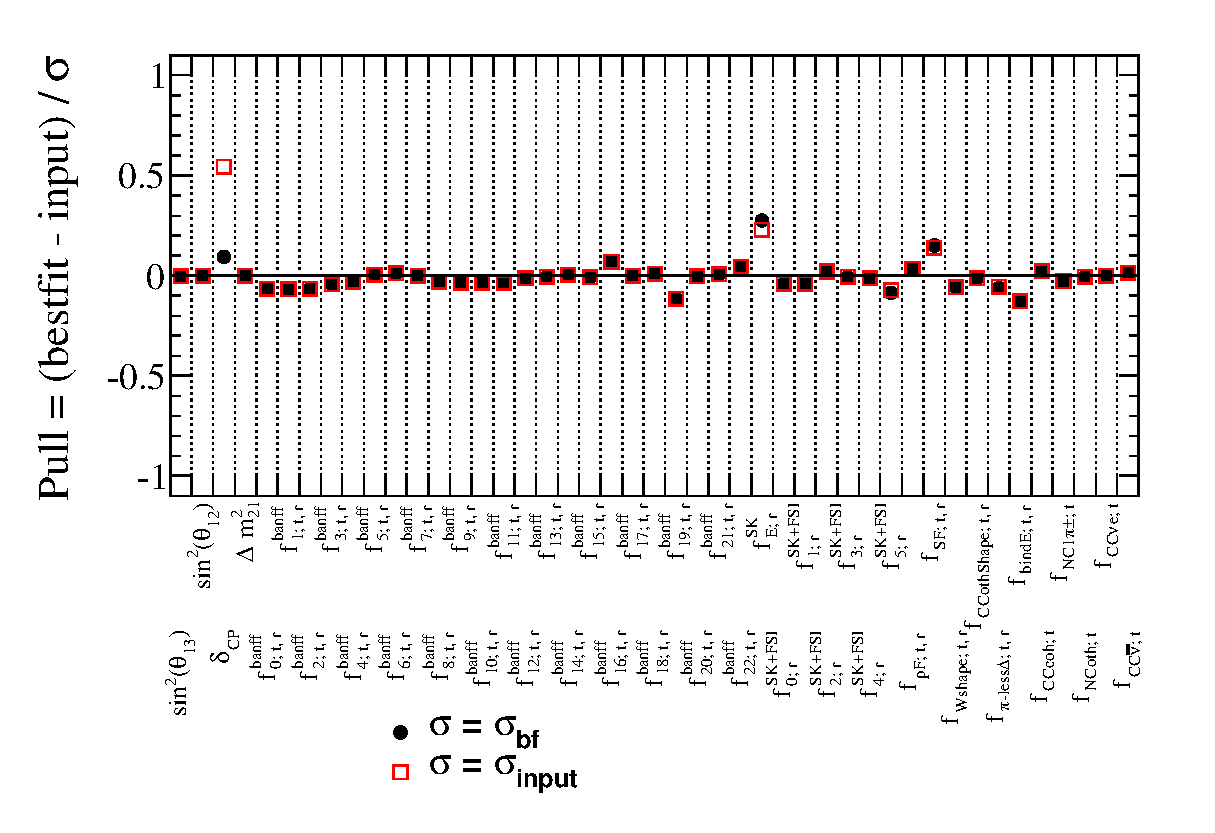
\includegraphics[width=50pc,angle=270]{./images/data_fit/normal/run1-4_nuis4_sintheta_normal_pulls_and_values}
\caption {
  Systematic parameter pulls from the fit of the Run 1+2+3+4 dataset.
  The normal mass hierarchy is assumed.
}
\label{fig:results_data1234_pulls:normal}
\end{figure*}

\begin{figure*}[htb]
\center
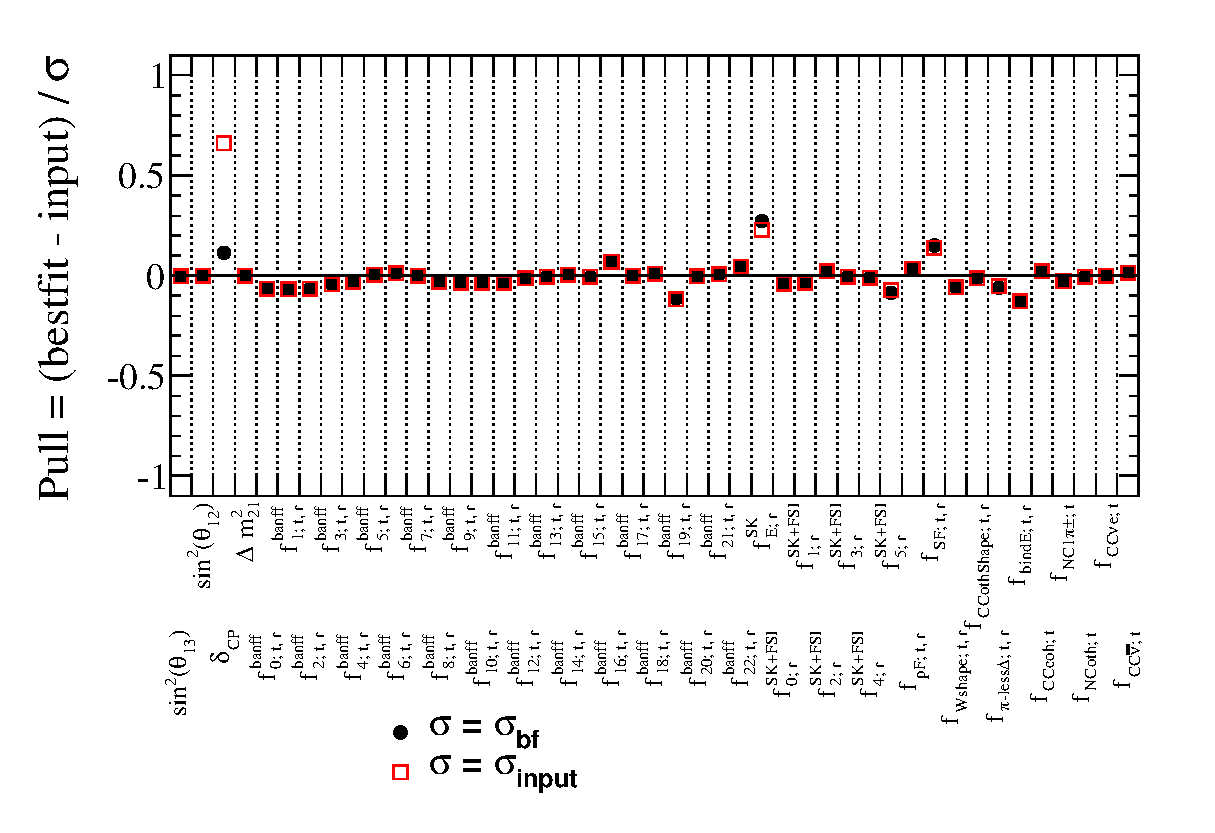
\includegraphics[width=50pc,angle=270]{./images/data_fit/inverted31/run1-4_nuis4_sintheta_inverted31_pulls_and_values}
\caption {
  Systematic parameter pulls from the fit of the Run 1+2+3+4 dataset.
  The inverted mass hierarchy is assumed.
}
\label{fig:results_data1234_pulls:inverted}
\end{figure*}

\begin{figure*}[htb]
  \begin{minipage}[t]{0.48\linewidth}
    \center
    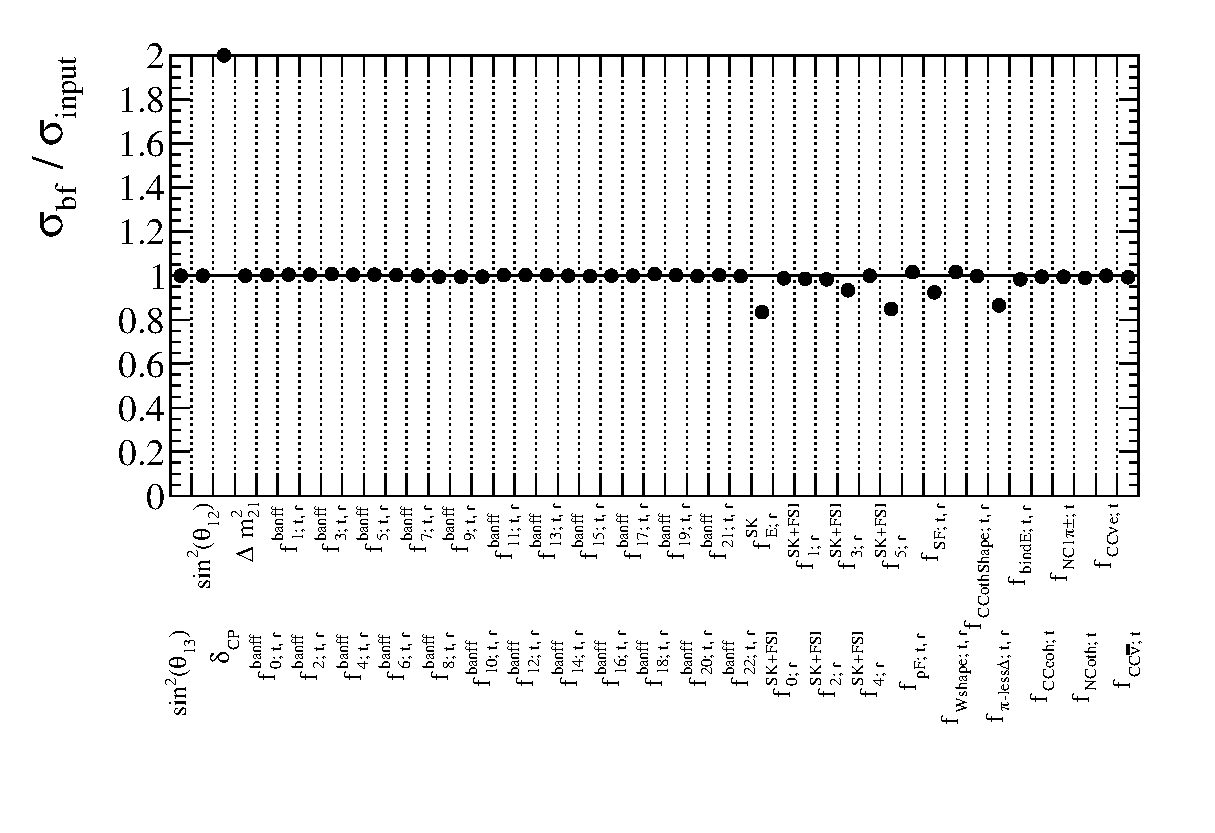
\includegraphics[width=28pc,angle=270]{./images/data_fit/normal/run1-4_nuis4_sintheta_normal_err_ratio}
    \caption {
      Ratio of $\sigma_{bestfit}$ / $\sigma_{input}$ from the fit of the Run 1+2+3+4 dataset.
      The normal mass hierarchy is assumed.
    }
    \label{fig:results_data1234_errratio:normal}
  \end{minipage}
  \hspace{0.06\linewidth}
  \begin{minipage}[t]{0.48\linewidth}
    \center
    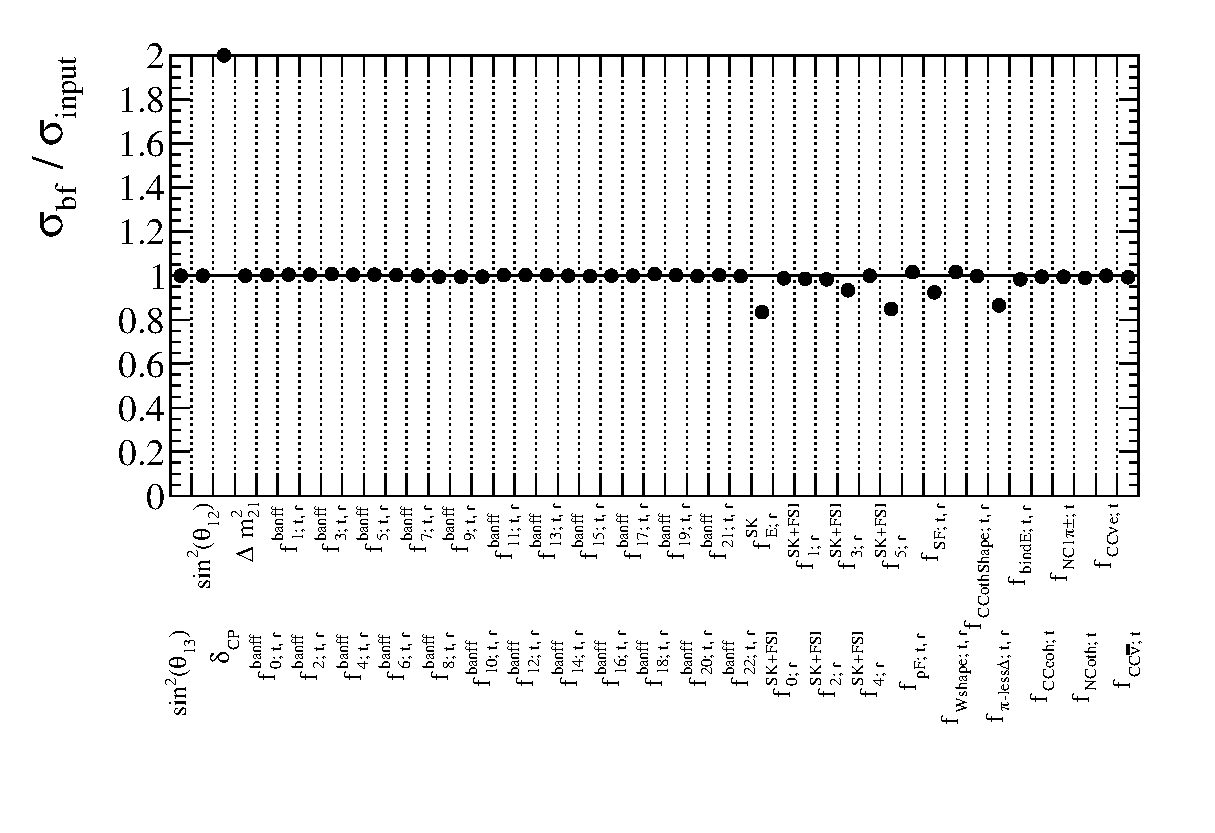
\includegraphics[width=28pc,angle=270]{./images/data_fit/inverted31/run1-4_nuis4_sintheta_inverted31_err_ratio}
    \caption {
      Ratio of $\sigma_{bestfit}$ / $\sigma_{input}$ from the fit of the Run 1+2+3+4 dataset.
      The inverted mass hierarchy is assumed.
    }
    \label{fig:results_data1234_errratio:inverted}
  \end{minipage}
\end{figure*}

%--------------------------------------------------------------------------------------
% Goodness of fit tests
%--------------------------------------------------------------------------------------

\subsection {Goodness-of-fit tests}
\label{sec:results_gof}

Goodness-of-fit tests were performed as described in Sec.\ \ref{sec:gof_test}, %\ 4.2 of Ref. \cite{OurRun123DisappAnalysis3Flavour},
and the p-values from the fits of the Run 1+2+3+4 dataset %, Run 1+2+3 and Run 4 datasets
are shown in Tab.\ \ref{tab:data_fits:best_fit_values}. 
The $\chi^2$ distributions from which these p-values were calculated are shown for the 
Run 1+2+3+4 data in Figs.\ \ref{fig:results_data1234_goodness:normal} and \ref{fig:results_data1234_goodness:inverted}
for the normal and inverted mass hierarchies respectively.
Both %All
fits have a high degree of plausibility.

%..................................
%
% Chisq_{gof} distributions
% 

\begin{figure*}[htb]
  \centering{
    \begin{minipage}[t]{0.8\linewidth}
      \center
      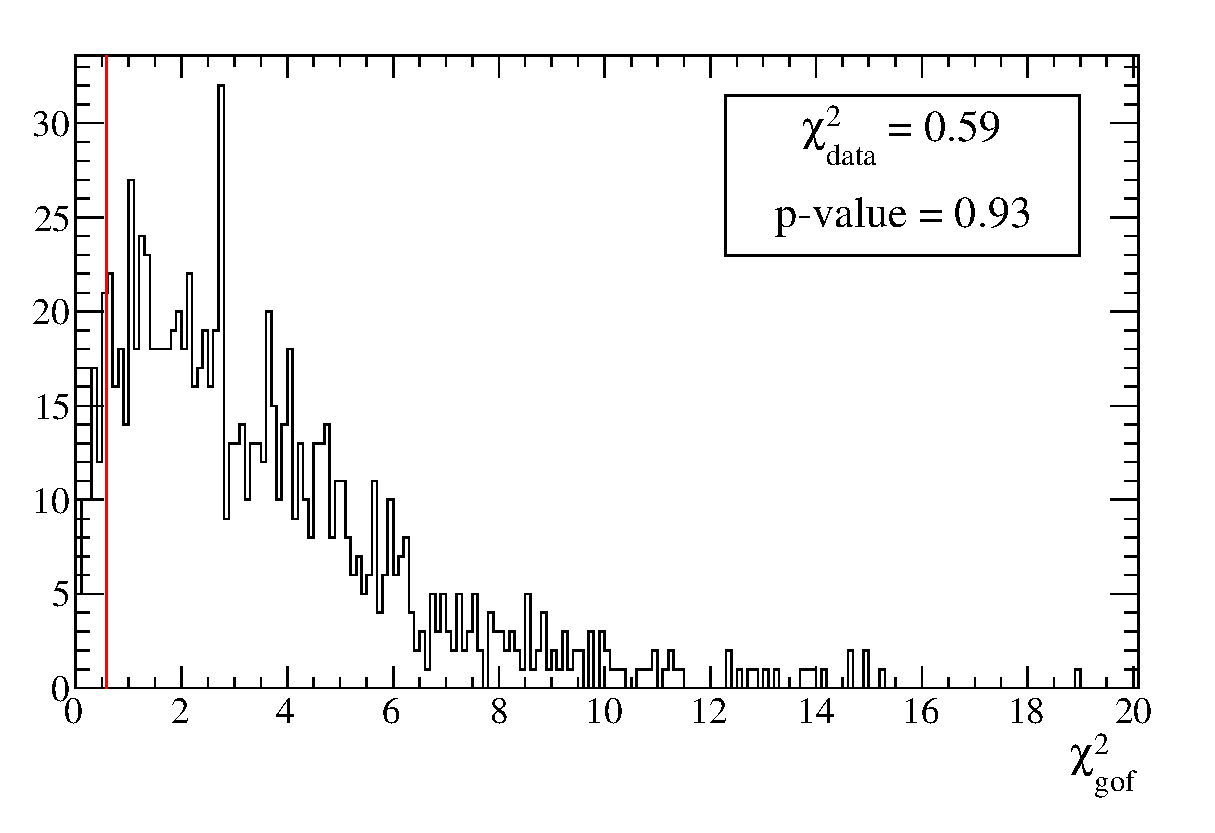
\includegraphics[width=24pc]{./images/data_fit/normal/goodness_run1-4_nuis4_sintheta_normal}
      \caption {
        Distribution of $\chi^2_{gof}$, the goodness-of-fit (gof) $\chi^2$, 
        from 1k toy MC experiments whose true input values were the Run 1+2+3+4 best-fit oscillation parameters.
        The $\chi^2_{gof}$ value from the fit of the Run 1+2+3+4 data ($\chi^2_{data}$) is highlighted.
        The normal mass hierarchy is assumed.
      }
      \label{fig:results_data1234_goodness:normal}
    \end{minipage}
    \vfill
    \begin{minipage}[t]{0.8\linewidth}

      \center
      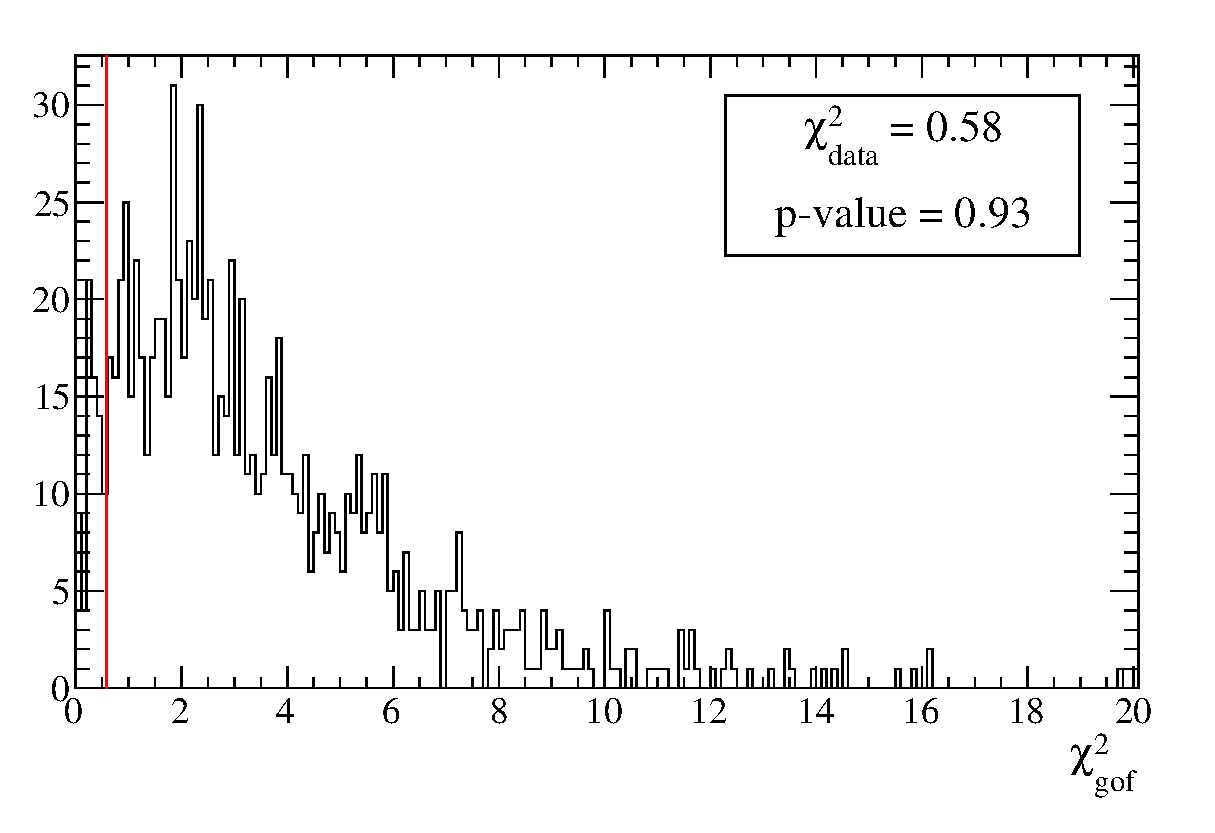
\includegraphics[width=24pc]{./images/data_fit/inverted31/goodness_run1-4_nuis4_sintheta_inverted31}
      \caption {
        Distribution of $\chi^2_{gof}$, the goodness-of-fit (gof) $\chi^2$, 
        from 1k toy MC experiments whose true input values were the Run 1+2+3+4 best-fit oscillation parameters.
        The $\chi^2_{gof}$ value for the fit of the Run 1+2+3+4 data ($\chi^2_{data}$) is highlighted.
        The inverted mass hierarchy is assumed.
      }
      \label{fig:results_data1234_goodness:inverted}
    \end{minipage}
  }
\end{figure*}


%--------------------------------------------------------------------------------------
% Best-fit spectra
%--------------------------------------------------------------------------------------

\subsection {Best-fit single-ring $\mu$-like reconstructed energy spectra}
\label{sec:results_bestfit_spectra}

The reconstructed neutrino energy distribution of the single $\mu$-like ring events in the Run 1+2+3+4 dataset 
is shown in Fig.\  \ref{fig:results_data1234_spectrum:normal} along with the best-fit predicted spectrum assuming 
the normal mass hierarchy and the predicted spectrum under the no-oscillation hypothesis. Also shown is the ratio of 
the data to the no-oscillation spectrum and the ratio of the best-fit spectrum to the no-oscillation spectrum; 
in both of these ratios, the characteristic energy-dependent deficit can be clearly seen.
The corresponding spectra for the fit assuming the inverted mass hierarchy are shown in Fig.\ \ref{fig:results_data1234_spectrum:inverted}.
The equivalent spectra for the Run 1+2+3 and Run 4 datasets are also shown in 
Figs.\ \ref{fig:results_data123_spectrum} and \ref{fig:results_data4_spectrum} respectively. 
All these distributions are shown in the 73-bin scheme in reconstructed 
neutrino energy that was used in the fitting procedure (see Sec.\ \ref{sec:mc_templates:template_binning}).

Since the reconstructed energy binning used in the fit is relatively fine, it can be beneficial to see the above distributions using 
a coarser binning. The best-fit spectra obtained from the fits of the Run 1+2+3+4 %, Run 1+2+3 and Run 4 datasets are
dataset are 
shown using a coarser binning scheme\footnote{
  16 reconstructed energy bins arranged as follows:
  1 0.3-GeV bin from 0 - 0.3 GeV,
  8 0.1-GeV bins from 0.3 - 1.1 GeV,
  1 0.15-GeV bin from 1.1 GeV - 1.25 GeV,
  1 0.25-GeV bin from 1.25 - 1.5 GeV GeV,
  1 0.5-GeV bin from 1.5 - 2 GeV,
  2 1-GeV bin from 2-4 GeV,
  1 2-GeV bin from 4-6 GeV and
  1 bin above 6 GeV.
} 
in Figs.\
\ref{fig:results_data1234_spectrum_coarse:normal} and \ref{fig:results_data1234_spectrum_coarse:inverted}
for the normal and inverted mass hierarchies respectively. The best-fit spectra from the fits of 
the Run 1+2+3 and Run 4 datasets are also shown in Figs.\
\ref{fig:results_data123_spectrum_coarse} and
\ref{fig:results_data4_spectrum_coarse} respectively. 
It is interesting to see the components of the best-fit predicted spectrum, and these are shown in
Figs.\ \ref{fig:results_data1234_spectrum_components:normal} and \ref{fig:results_data1234_spectrum_components:inverted}
for the normal and inverted mass hierarchies respectively.
In these plots, the 32 components of the predicted spectrum are grouped into 5 categories: 
$\nu_{\mu}$ CCQE, $\nu_{\mu}$ CCnonQE, $\bar{\nu}_{\mu}$ CC, $\nu_{e}$/$\bar{\nu}_{e}$ CC and NC (though each of the 32 
components is calculated separately in the actual analysis).

The best-fit predicted spectra for the normal and inverted mass hierarchies are compared for the Run 1+2+3+4 dataset in
Fig.\ \ref{fig:results_data1234_spectrum_comparison},
using the 73 reconstructed energy bins used in the fit, and in
Fig. \ref{fig:results_data1234_spectrum_comparison_coarse},
using the coarser binning described above.
These two best-fit spectra are nearly identical.

Finally, the best-fit predicted spectra for the Run 1+2+3, Run 4, and Run 1+2+3+4 datasets,
all scaled to Run 1+2+3+4 POT, are compared for
the normal mass hierarchy in 
Fig.\ \ref{fig:results_dataruns_spectrum_comparison},
using the 73 reconstructed energy bins used in the fit, and in
Fig. \ref{fig:results_dataruns_spectrum_comparison_coarse},
using the coarser binning described above.
The spectra are consistent;
the largest differences below the oscillation maximum are consistent with a shift in $|\Delta m^2_{32}|$.

% {\color{red} We could also show a comparison between the 5 components listed above 
% and, also, show results of a test to check consistency between the 3 best-fit predictions}.

%...........................................................
%
% Best-fit spectra and ratios (73 bins)
%
\begin{figure*}[htb]
  \centering{
    \begin{minipage}[t]{0.8\linewidth}
      \center
      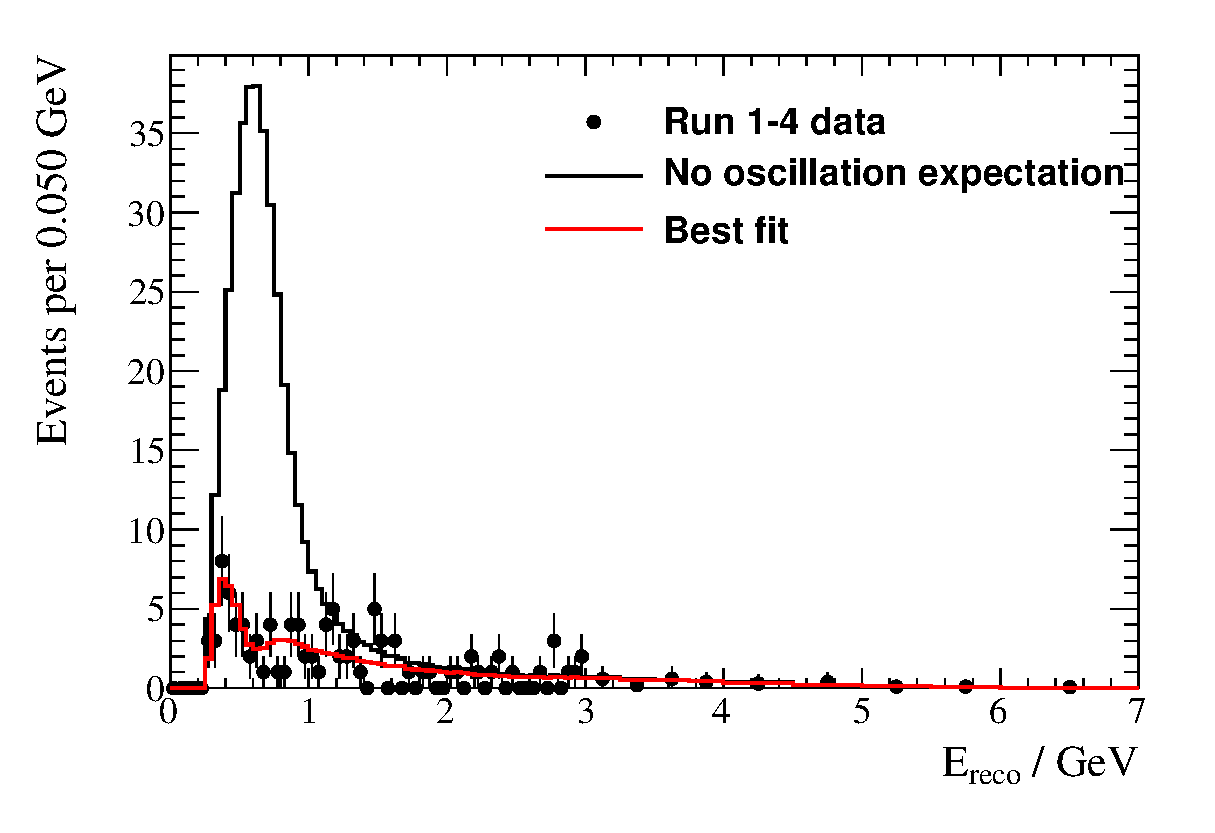
\includegraphics[width=28pc]{./images/data_fit/normal/run1-4_nuis4_sintheta_normal_spectrumper50}
    \end{minipage}
    \vfill
    \begin{minipage}[t]{0.8\linewidth}
      \center
      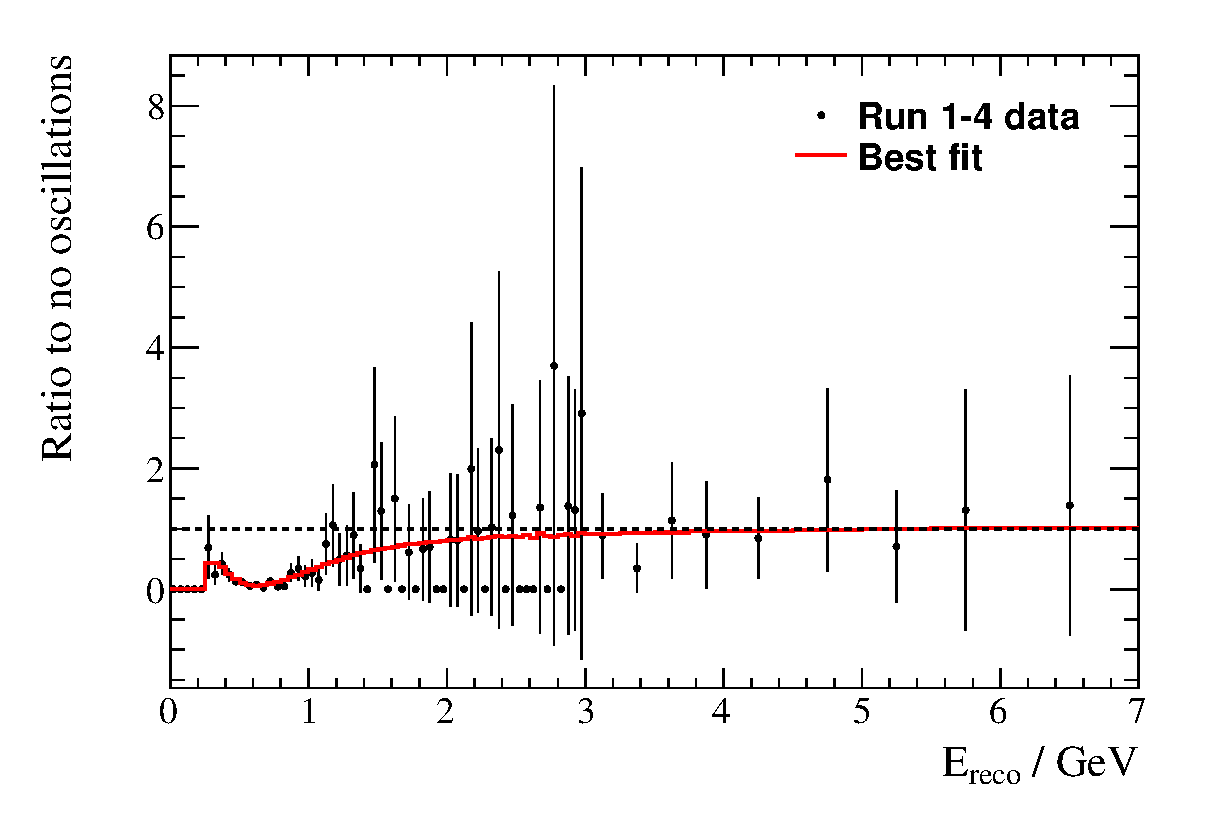
\includegraphics[width=28pc]{./images/data_fit/normal/run1-4_nuis4_sintheta_normal_spectrum_ratio}
    \end{minipage}
    \caption {
      Best-fit reconstructed energy spectrum (top) obtained from the fit of the combined Run 1+2+3+4 dataset.
      The Run 1+2+3+4 data and the prediction obtained using the no-oscillation hypothesis are also shown.
      The spectra are shown using the 73 bins used in the fit (see Sec.\ \ref{sec:mc_templates:template_binning}).
      The ratios of the data and best-fit predicted spectrum to the no-oscillation hypothesis are shown 
      in the lower plot. The characteristic energy-dependent deficit can be clearly seen.
      The normal mass hierarchy is assumed.
      \label{fig:results_data1234_spectrum:normal}
    }
  }
\end{figure*}

\begin{figure*}[htb]
  \centering{
    \begin{minipage}[t]{0.8\linewidth}
      \center
      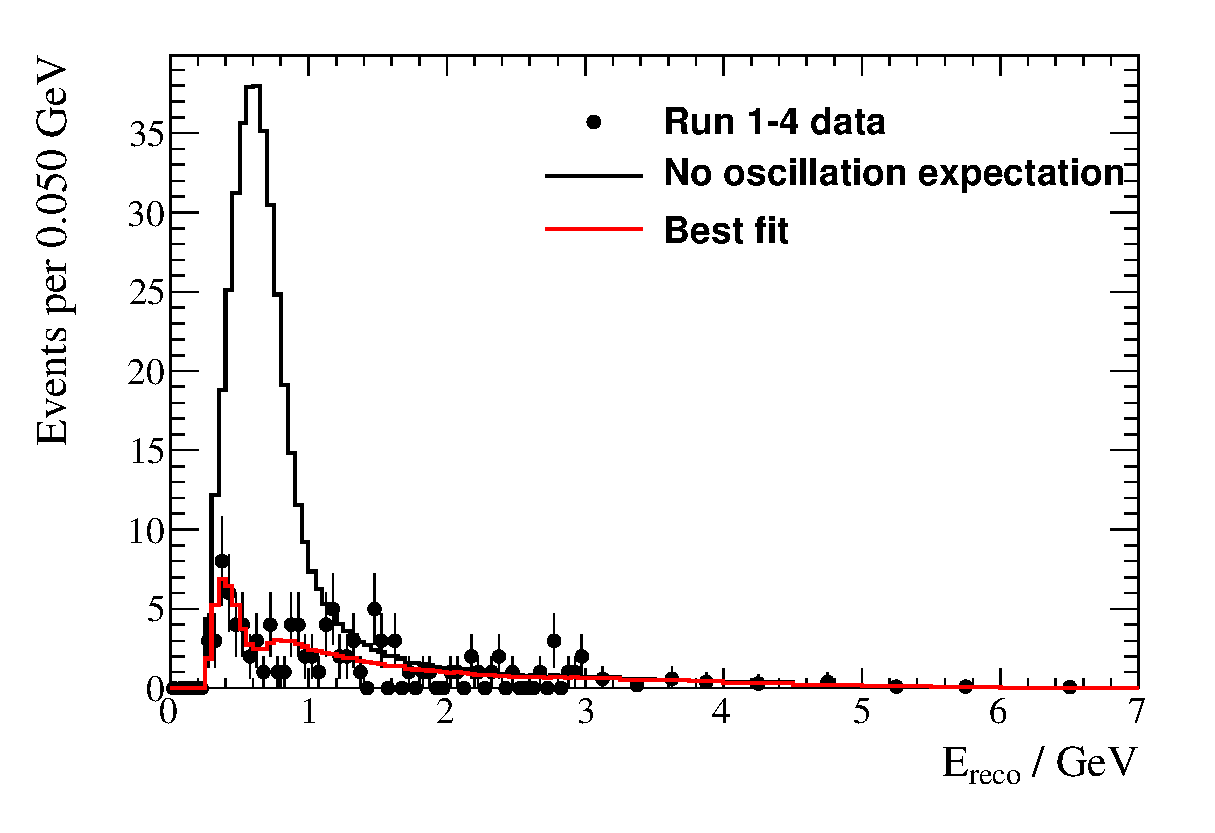
\includegraphics[width=28pc]{./images/data_fit/inverted31/run1-4_nuis4_sintheta_inverted31_spectrumper50}
    \end{minipage}
    \vfill
    \begin{minipage}[t]{0.8\linewidth}
      \center
      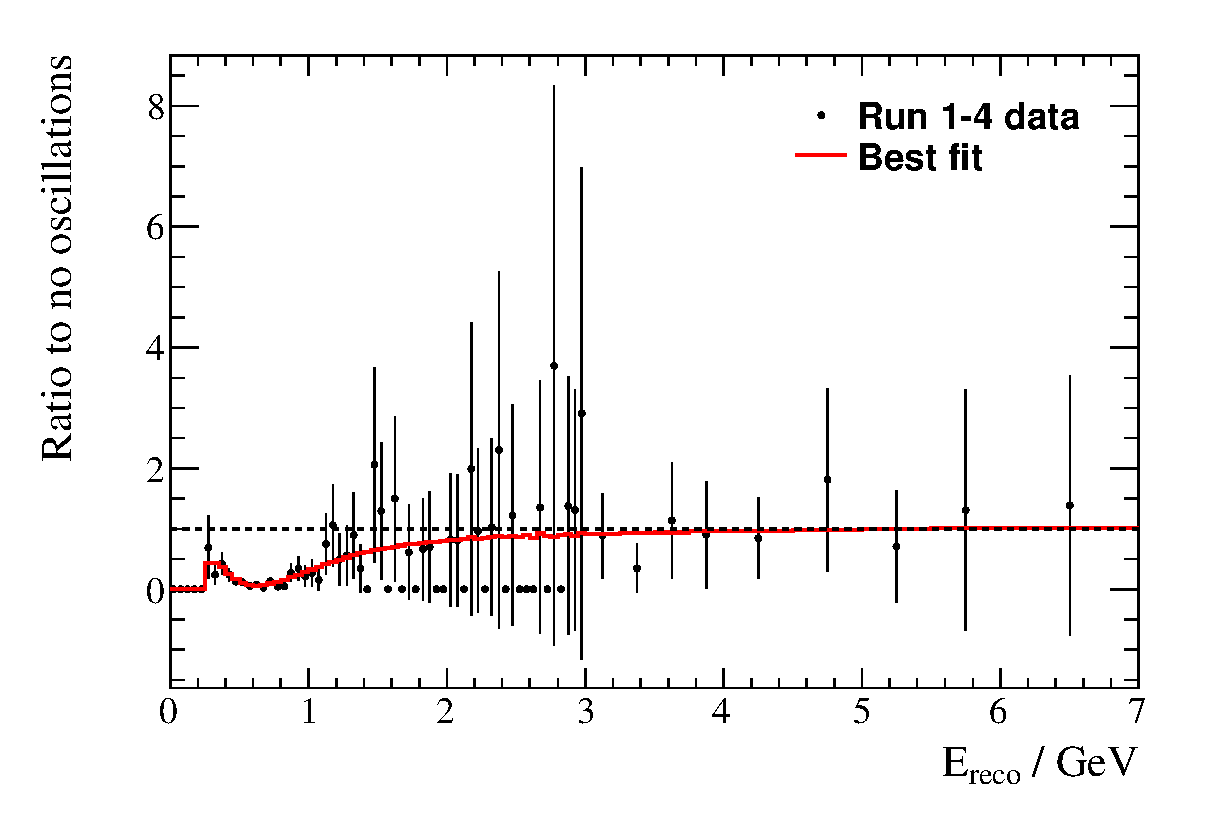
\includegraphics[width=28pc]{./images/data_fit/inverted31/run1-4_nuis4_sintheta_inverted31_spectrum_ratio}
    \end{minipage}
    \caption {
      Best-fit reconstructed energy spectrum (top) obtained from the fit of the combined Run 1+2+3+4 dataset.
      The Run 1+2+3+4 data and the prediction obtained using the no-oscillation hypothesis are also shown.
      The spectra are shown using the 73 bins used in the fit (see Sec.\ \ref{sec:mc_templates:template_binning}).
      The ratios of the data and best-fit predicted spectrum to the no-oscillation hypothesis are shown 
      in the lower plot. The characteristic energy-dependent deficit can be clearly seen.
      The inverted mass hierarchy is assumed.
      \label{fig:results_data1234_spectrum:inverted}
    }
  }
\end{figure*}

\begin{figure*}[htb]
  \begin{minipage}[t]{0.48\linewidth}
    \center
    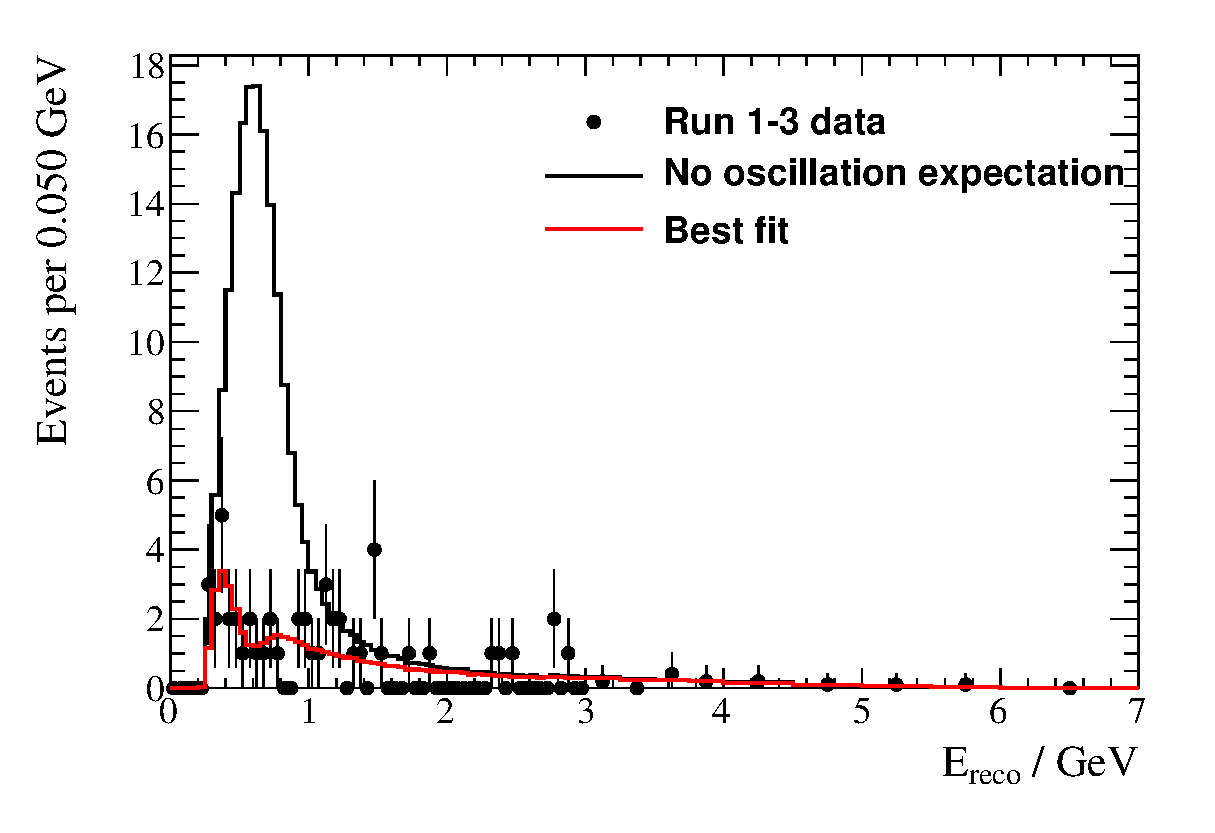
\includegraphics[width=20pc]{./images/data_fit/run123/run1-4_nuis4_sintheta_normal_run123_spectrumper50}
  \end{minipage}
  \hspace{0.06\linewidth}
  \begin{minipage}[t]{0.48\linewidth}
    \center
    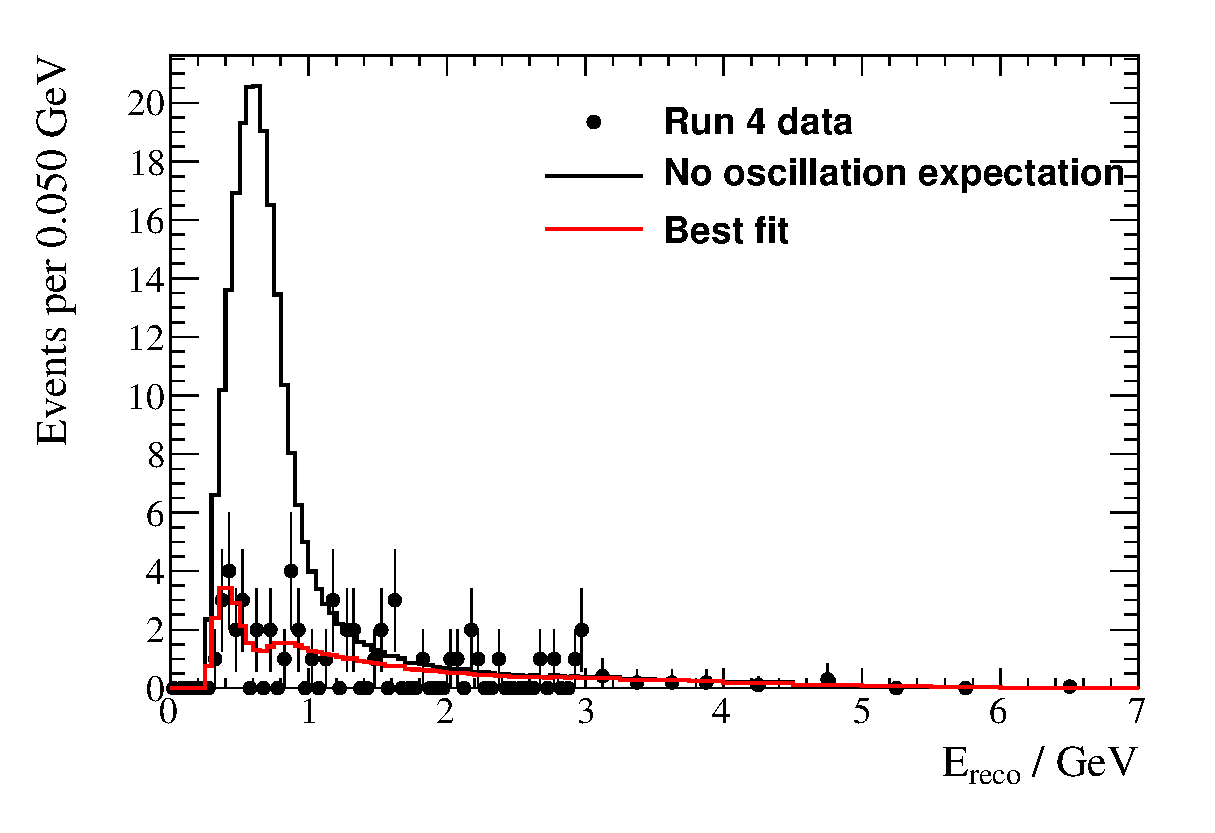
\includegraphics[width=20pc]{./images/data_fit/run4/run1-4_nuis4_sintheta_normal_run4_spectrumper50}
  \end{minipage}
  \vfill
  \begin{minipage}[t]{0.48\linewidth}
    \center
    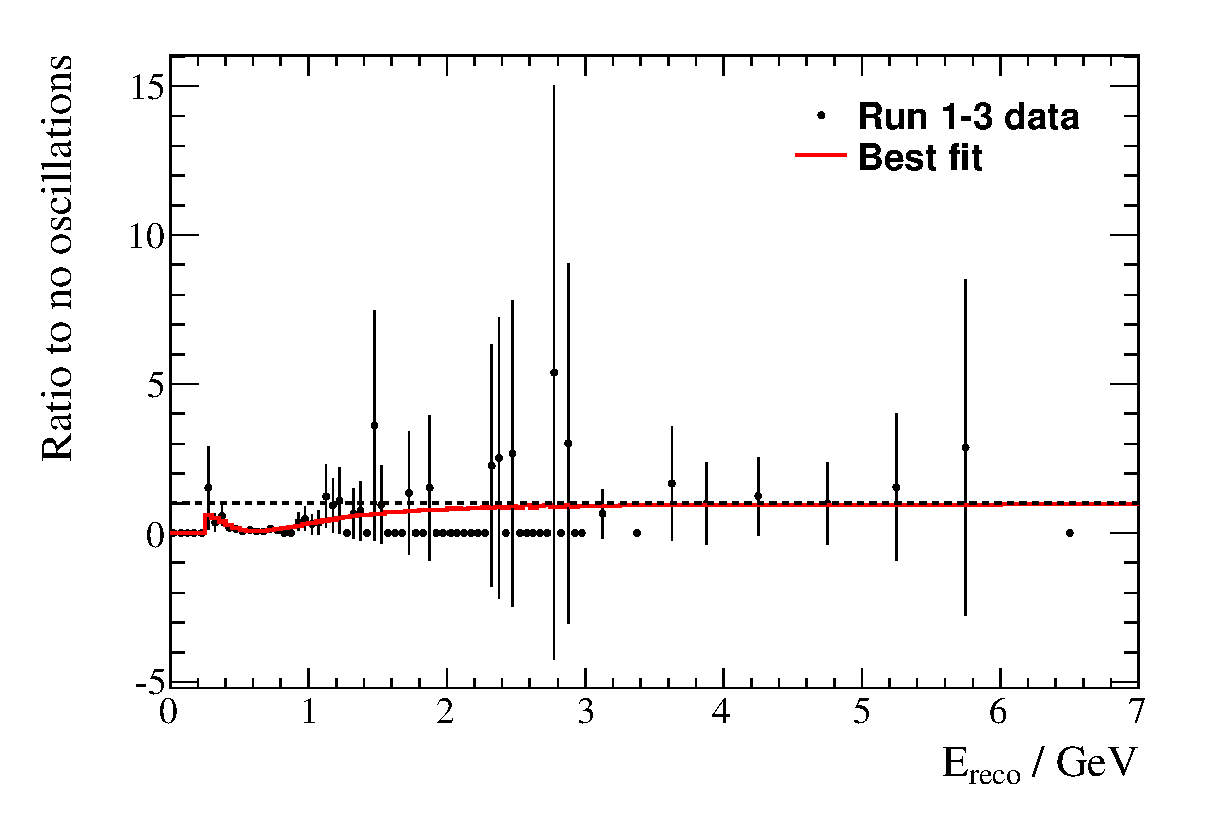
\includegraphics[width=20pc]{./images/data_fit/run123/run1-4_nuis4_sintheta_normal_run123_spectrum_ratio}
    \caption {
      Best-fit reconstructed energy spectrum (top) obtained from the fit of the Run 1+2+3 dataset only.
      The Run 1+2+3 data and the prediction obtained using the no-oscillation hypothesis are also shown.
      The spectra are shown using the 73 bins used in the fit (see Sec.\ \ref{sec:mc_templates:template_binning}).
      The ratios of the data and best-fit predicted spectrum to the no-oscillation hypothesis are shown
      in the lower plot. The characteristic energy-dependent deficit can be clearly seen.
      The normal mass hierarchy is assumed.
    }
    \label{fig:results_data123_spectrum}
  \end{minipage}
  \hspace{0.06\linewidth}
  \begin{minipage}[t]{0.48\linewidth}
    \center
    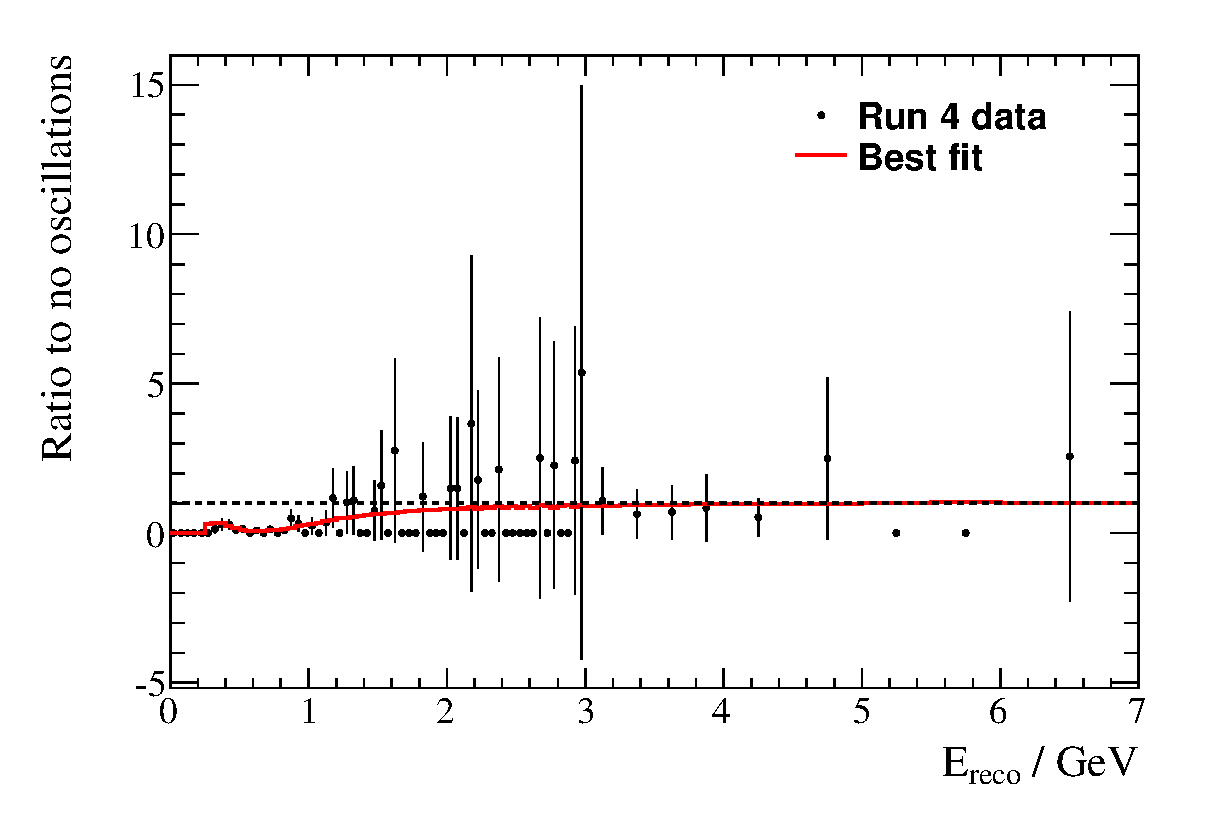
\includegraphics[width=20pc]{./images/data_fit/run4/run1-4_nuis4_sintheta_normal_run4_spectrum_ratio}
    \caption {
      Best-fit reconstructed energy spectrum (top) obtained from the fit of the combined Run 4 dataset only.
      The Run 4 data and the prediction obtained using the no-oscillation hypothesis are also shown.
      The spectra are shown using the 73 bins used in the fit (see Sec.\ \ref{sec:mc_templates:template_binning}).
      The ratios of the data and best-fit predicted spectrum to the no-oscillation hypothesis are shown
      in the lower plot. The characteristic energy-dependent deficit can be clearly seen.
      The normal mass hierarchy is assumed.
    }
    \label{fig:results_data4_spectrum}
  \end{minipage}
\end{figure*}

%...........................................................
%
% Best-fit spectra and ratios (coarse binning)
%
\begin{figure*}[htb]
  \centering{
    \begin{minipage}[t]{0.8\linewidth}
      \center
      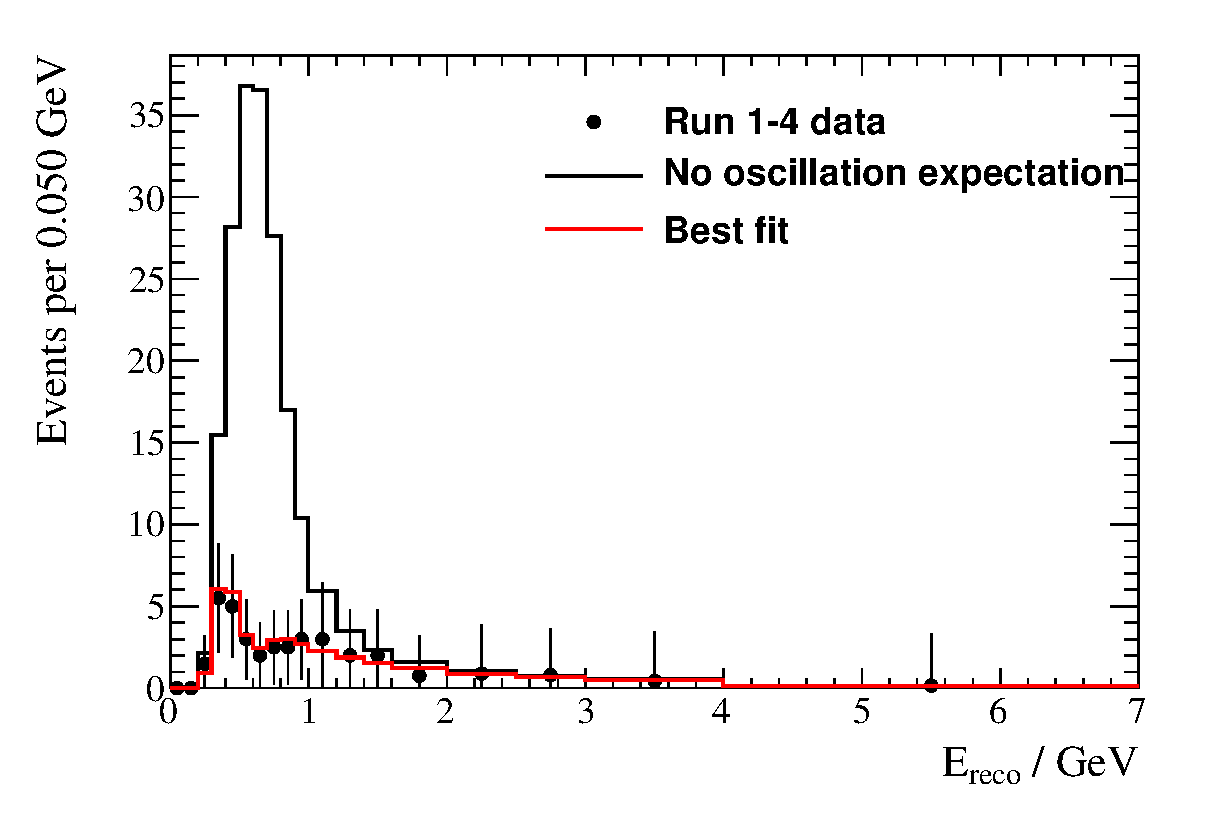
\includegraphics[width=28pc]{./images/data_fit/normal/run1-4_nuis4_sintheta_normal_spectrumper50_rebin}
    \end{minipage}
    \vfill
    \begin{minipage}[t]{0.8\linewidth}
      \center
      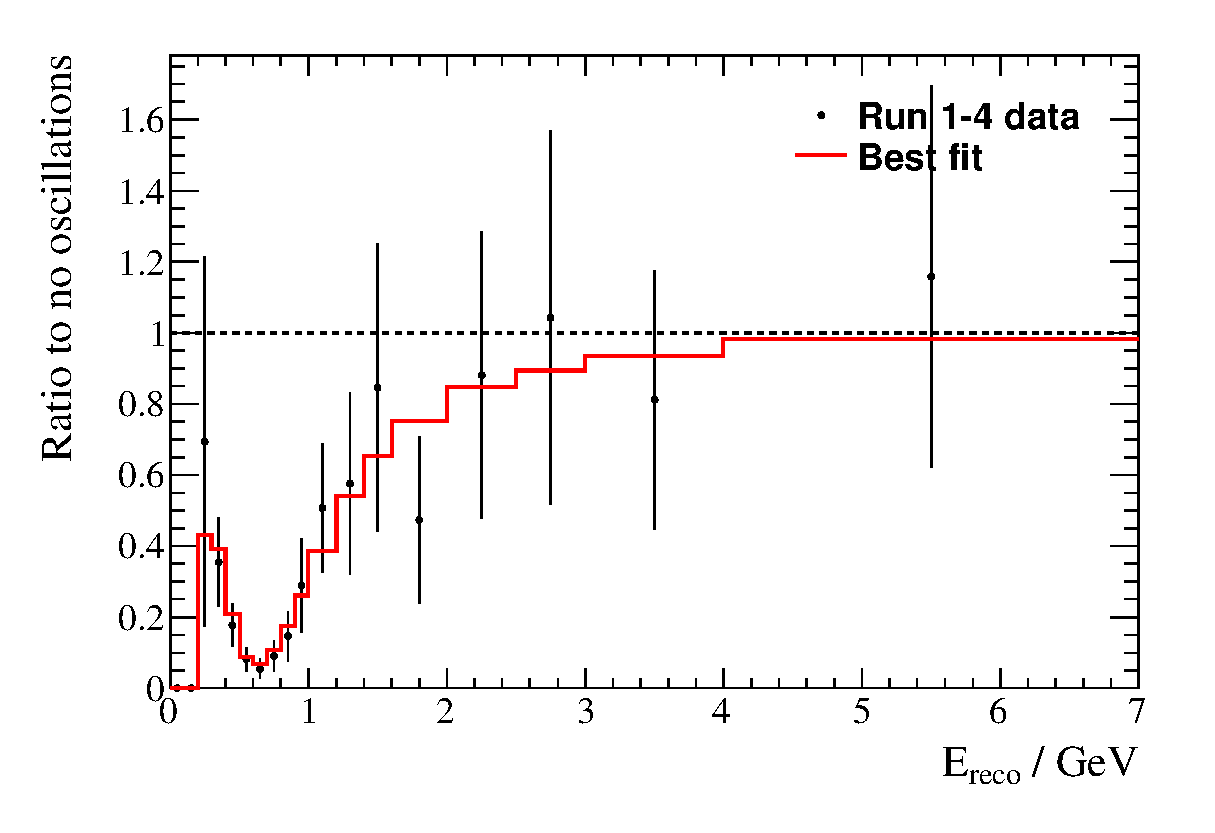
\includegraphics[width=28pc]{./images/data_fit/normal/run1-4_nuis4_sintheta_normal_spectrum_ratio_rebin}
    \end{minipage}
    \caption {
      Best-fit reconstructed energy spectrum (top) obtained from the fit of the combined Run 1+2+3+4 dataset.
      The Run 1+2+3+4 data and the prediction obtained using the no-oscillation hypothesis are also shown.
      The spectra are shown using the coarse binning scheme described in Sec.\ \ref{sec:results_bestfit_spectra}.
      The characteristic energy-dependent deficit can be clearly seen.
      The normal mass hierarchy is assumed.
      \label{fig:results_data1234_spectrum_coarse:normal}
    }
  }
\end{figure*}

\begin{figure*}[htb]
  \centering{
    \begin{minipage}[t]{0.8\linewidth}
      \center
      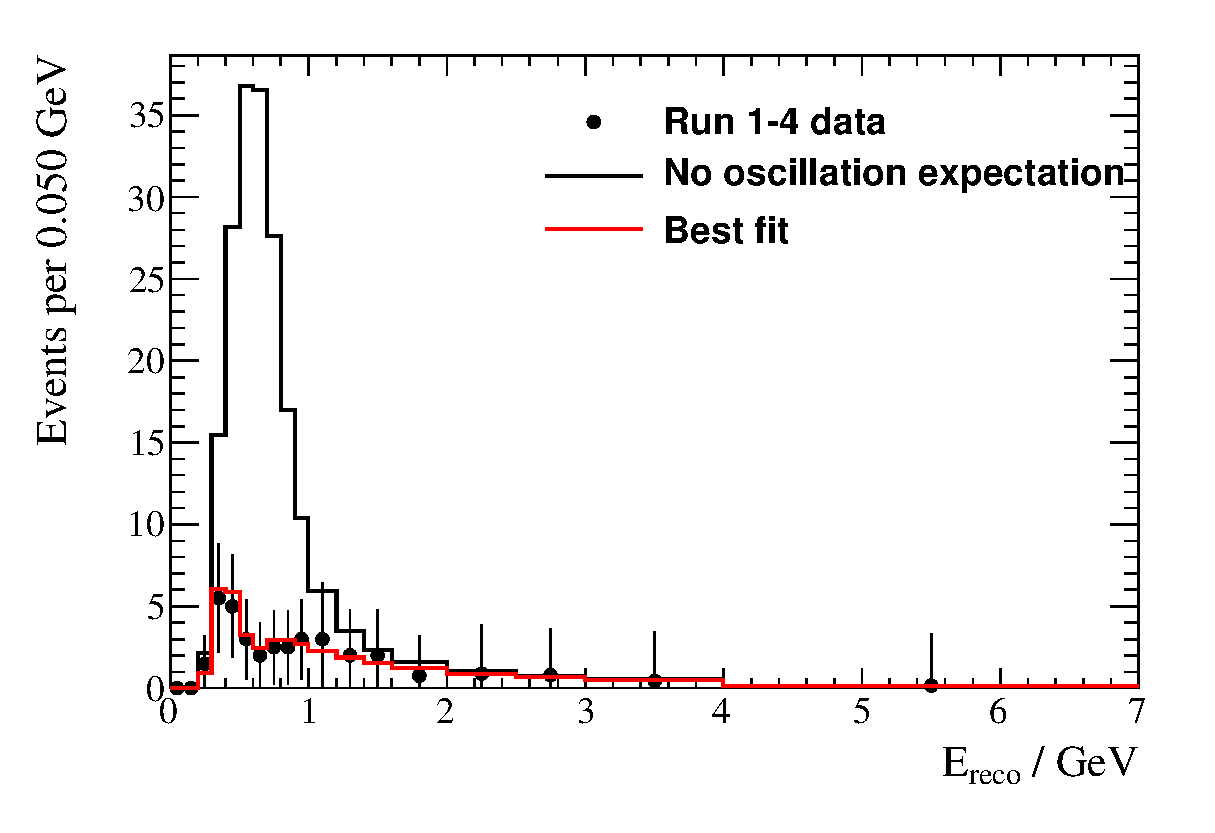
\includegraphics[width=28pc]{./images/data_fit/inverted31/run1-4_nuis4_sintheta_inverted31_spectrumper50_rebin}
    \end{minipage}
    \vfill
    \begin{minipage}[t]{0.8\linewidth}
      \center
      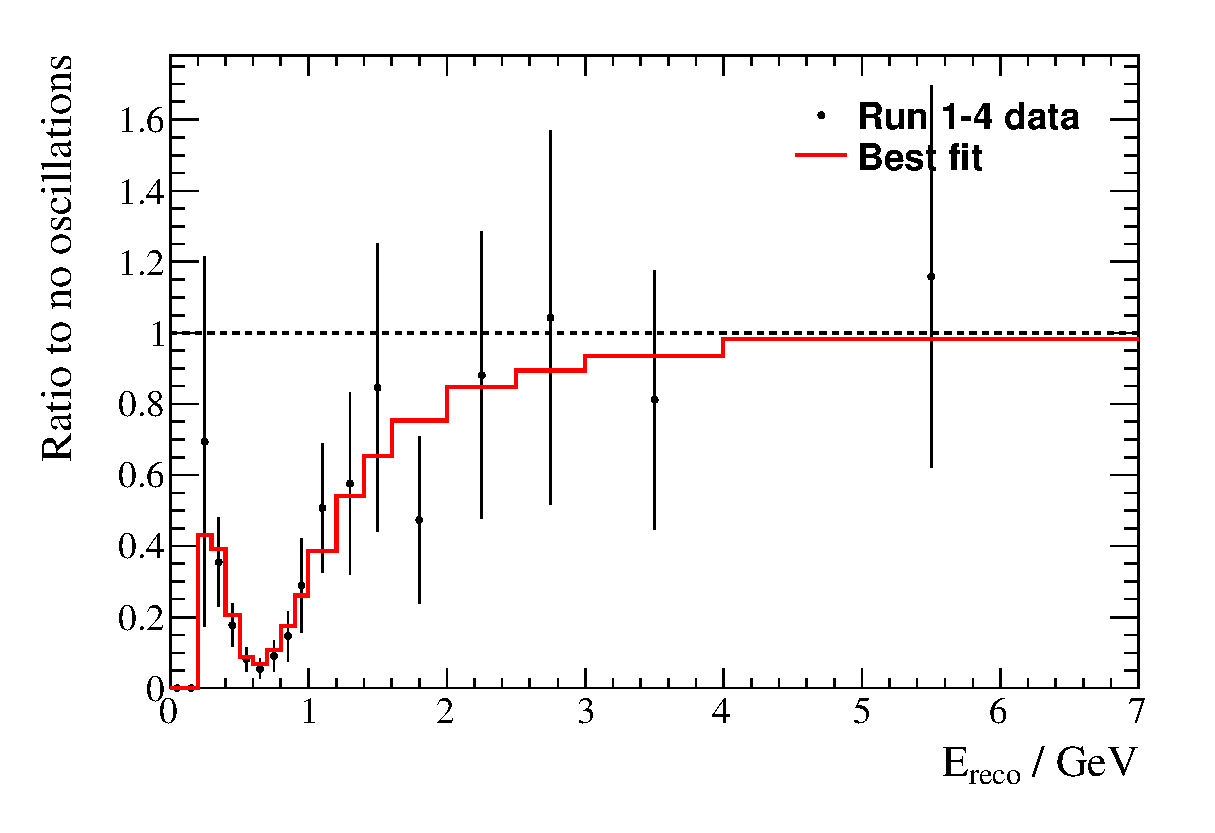
\includegraphics[width=28pc]{./images/data_fit/inverted31/run1-4_nuis4_sintheta_inverted31_spectrum_ratio_rebin}
    \end{minipage}
    \caption {
      Best-fit reconstructed energy spectrum (top) obtained from the fit of the combined Run 1+2+3+4 dataset.
      The Run 1+2+3+4 data and the prediction obtained using the no-oscillation hypothesis are also shown.
      The spectra are shown using the coarse binning scheme described in Sec.\ \ref{sec:results_bestfit_spectra}.
      The characteristic energy-dependent deficit can be clearly seen.
      The inverted mass hierarchy is assumed.
      \label{fig:results_data1234_spectrum_coarse:inverted}
    }
  }
\end{figure*}

\begin{figure*}[htb]
  \begin{minipage}[t]{0.48\linewidth}
    \center
    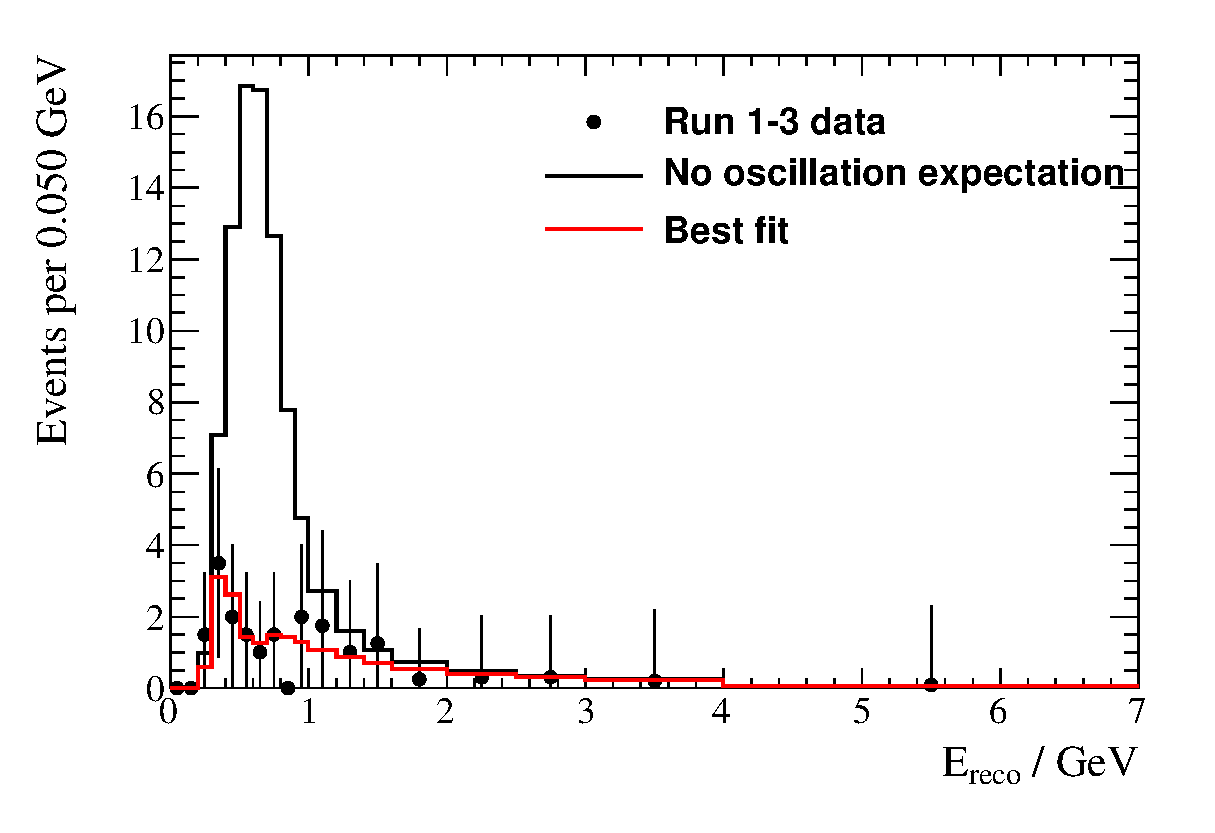
\includegraphics[width=20pc]{./images/data_fit/run123/run1-4_nuis4_sintheta_normal_run123_spectrumper50_rebin}
  \end{minipage}
  \hspace{0.06\linewidth}
  \begin{minipage}[t]{0.48\linewidth}
    \center
    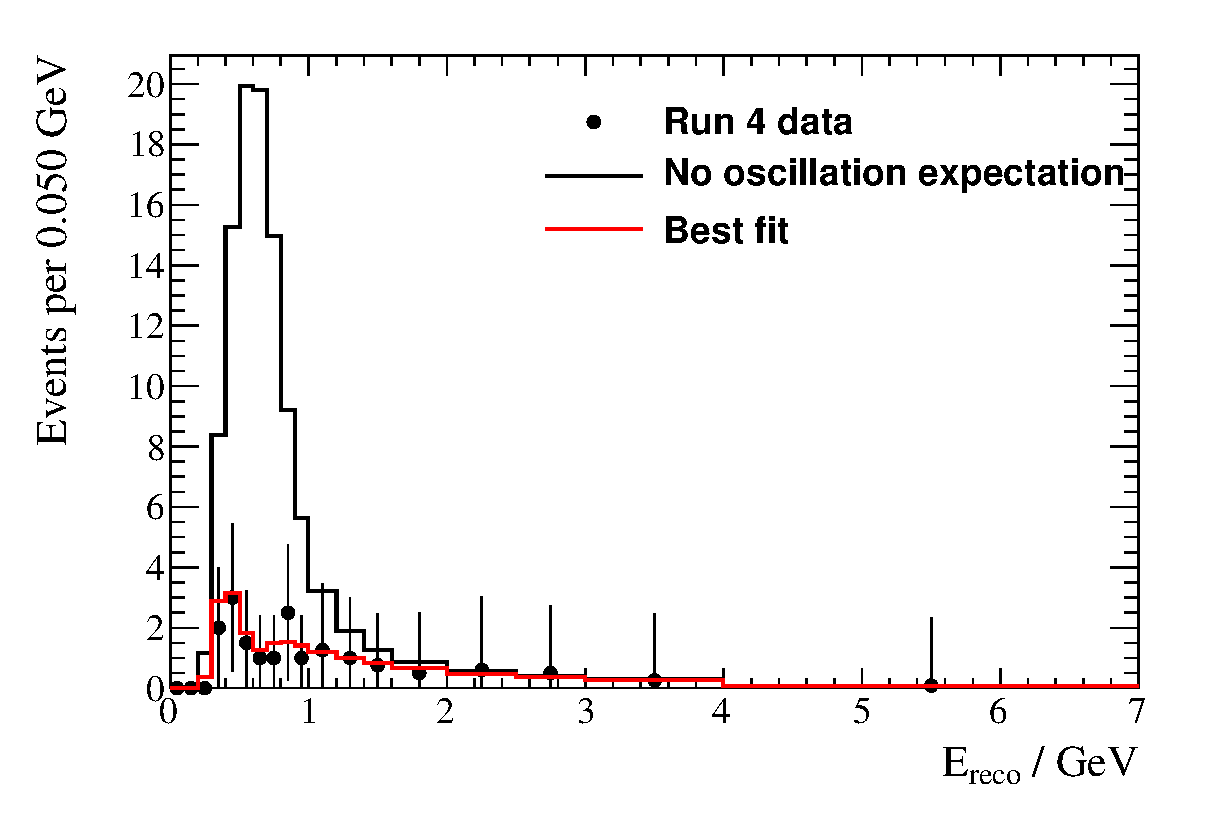
\includegraphics[width=20pc]{./images/data_fit/run4/run1-4_nuis4_sintheta_normal_run4_spectrumper50_rebin}
  \end{minipage}
  \vfill
  \begin{minipage}[t]{0.48\linewidth}
    \center
    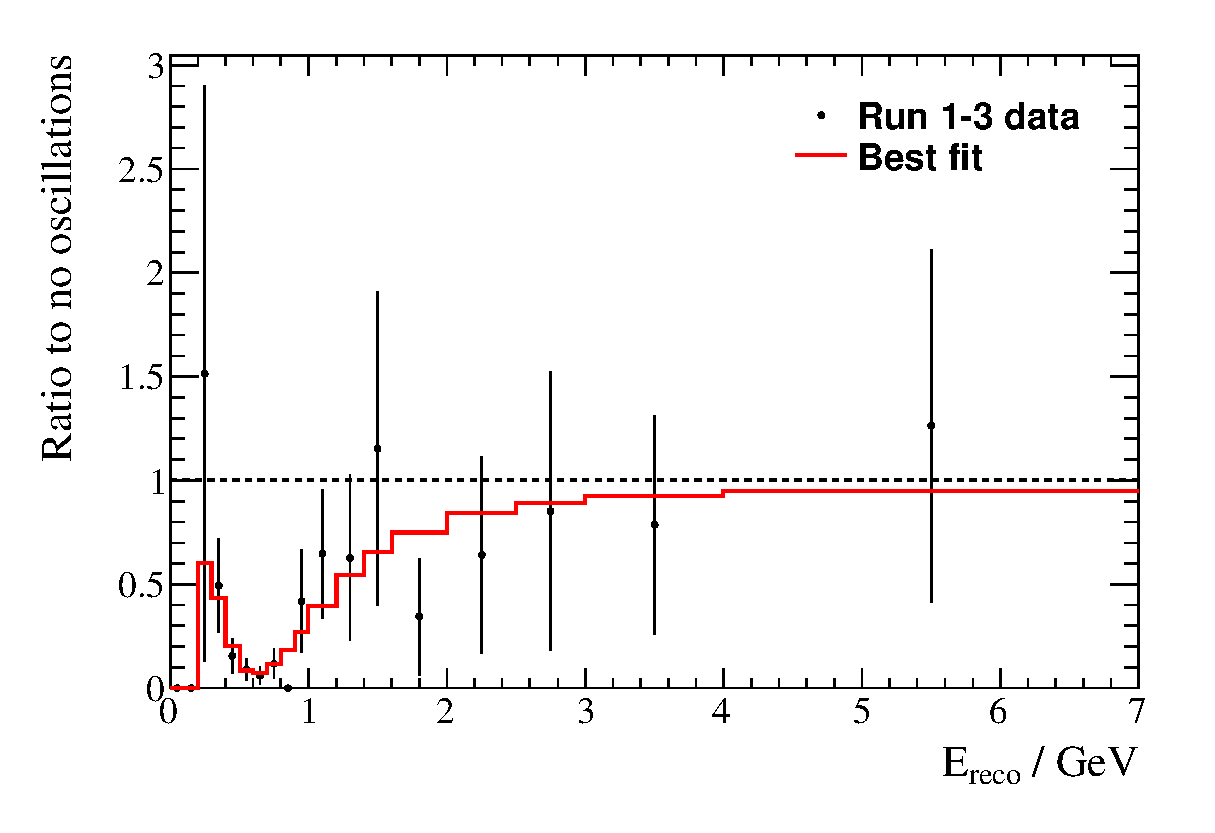
\includegraphics[width=20pc]{./images/data_fit/run123/run1-4_nuis4_sintheta_normal_run123_spectrum_ratio_rebin}
    \caption {
      Best-fit reconstructed energy spectrum (top) obtained from the fit of the combined Run 1+2+3 dataset only.
      The Run 1+2+3 data and the prediction obtained using the no-oscillation hypothesis are also shown.
      The spectra are shown using the coarse binning scheme described in Sec.\ \ref{sec:results_bestfit_spectra}.
      The characteristic energy-dependent deficit can be clearly seen.
      The normal mass hierarchy is assumed.
    }
    \label{fig:results_data123_spectrum_coarse}
  \end{minipage}
  \hspace{0.06\linewidth}
  \begin{minipage}[t]{0.48\linewidth}
    \center
    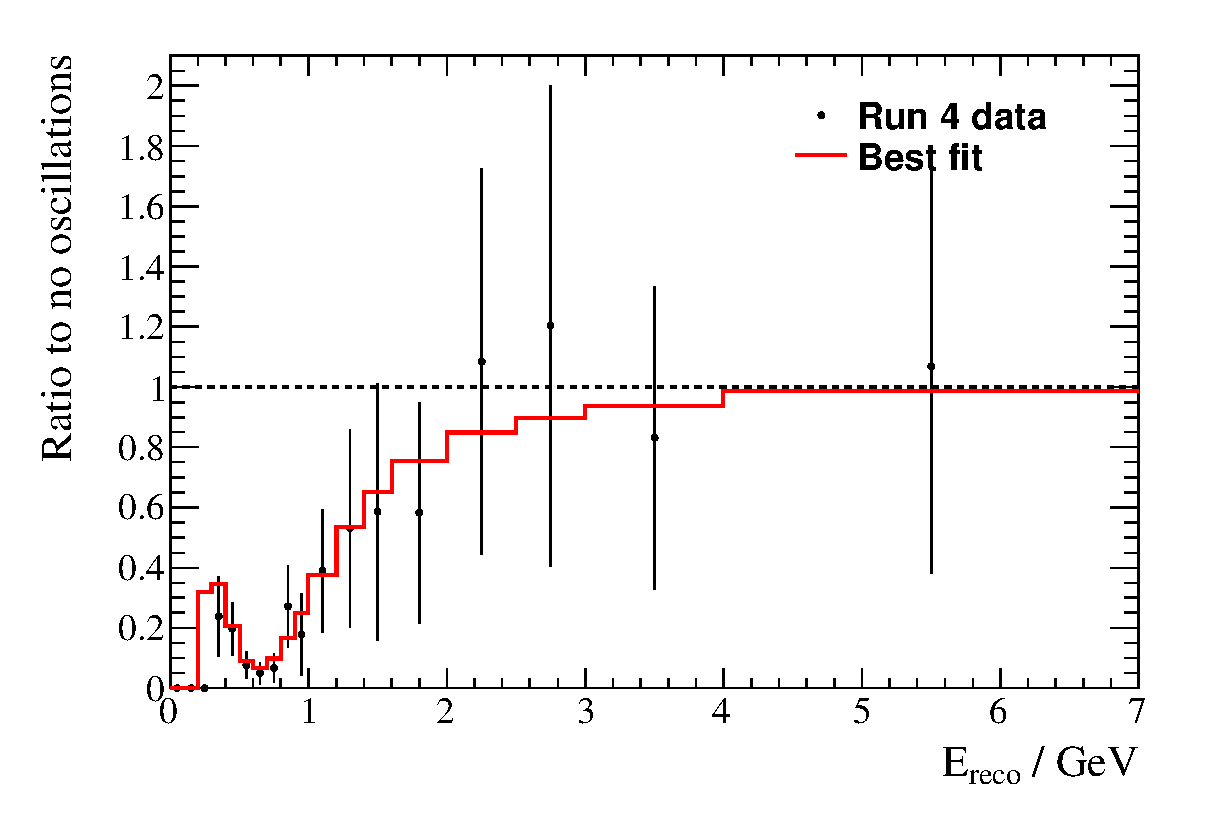
\includegraphics[width=20pc]{./images/data_fit/run4/run1-4_nuis4_sintheta_normal_run4_spectrum_ratio_rebin}
    \caption {
      Best-fit reconstructed energy spectrum (top) obtained from the fit of the combined Run 4 dataset only.
      The Run 4 data and the prediction obtained using the no-oscillation hypothesis are also shown.
      The spectra are shown using the coarse binning scheme described in Sec.\ \ref{sec:results_bestfit_spectra}.
      The characteristic energy-dependent deficit can be clearly seen.
      The normal mass hierarchy is assumed.
    }
    \label{fig:results_data4_spectrum_coarse}
  \end{minipage}
\end{figure*}


%...........................................................
%
% Best-fit spectra (total and components) for `2+N' fit 
% (Run1+2+3+4 only, 73 bins)
%

\begin{figure*}[htb]
  \center
  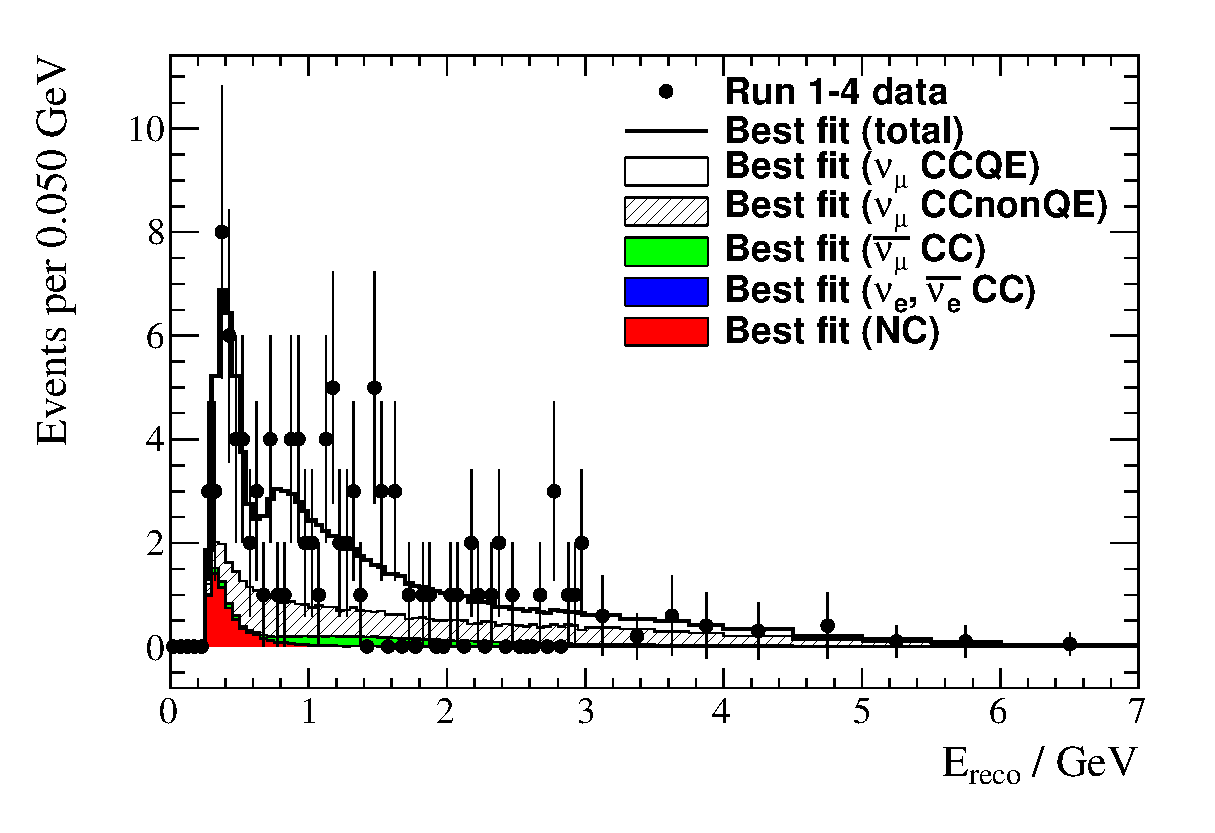
\includegraphics[width=28pc]{./images/data_fit/normal/run1-4_nuis4_sintheta_normal_spectrumper50_components}
  \caption {
    Best-fit reconstructed energy spectrum in the 73-bin scheme used in the fit (see Sec.\ref{sec:mc_templates:template_binning})
    and its components
    obtained from the fit of the Run 1+2+3+4 dataset.  
    The 32 components, each of which is calculated separately in the analysis, are grouped into just 5 categories:
    $\nu_{\mu}$ CCQE, $\nu_{\mu}$ CCnQE, $\bar{\nu_{\mu}}$ CC, $\nu_{e}$/$\bar{\nu_{e}}$ CC and NC.  
    The normal mass hierarchy is assumed.
  }
  \label{fig:results_data1234_spectrum_components:normal}
\end{figure*}

\begin{figure*}[htb]
  \center
  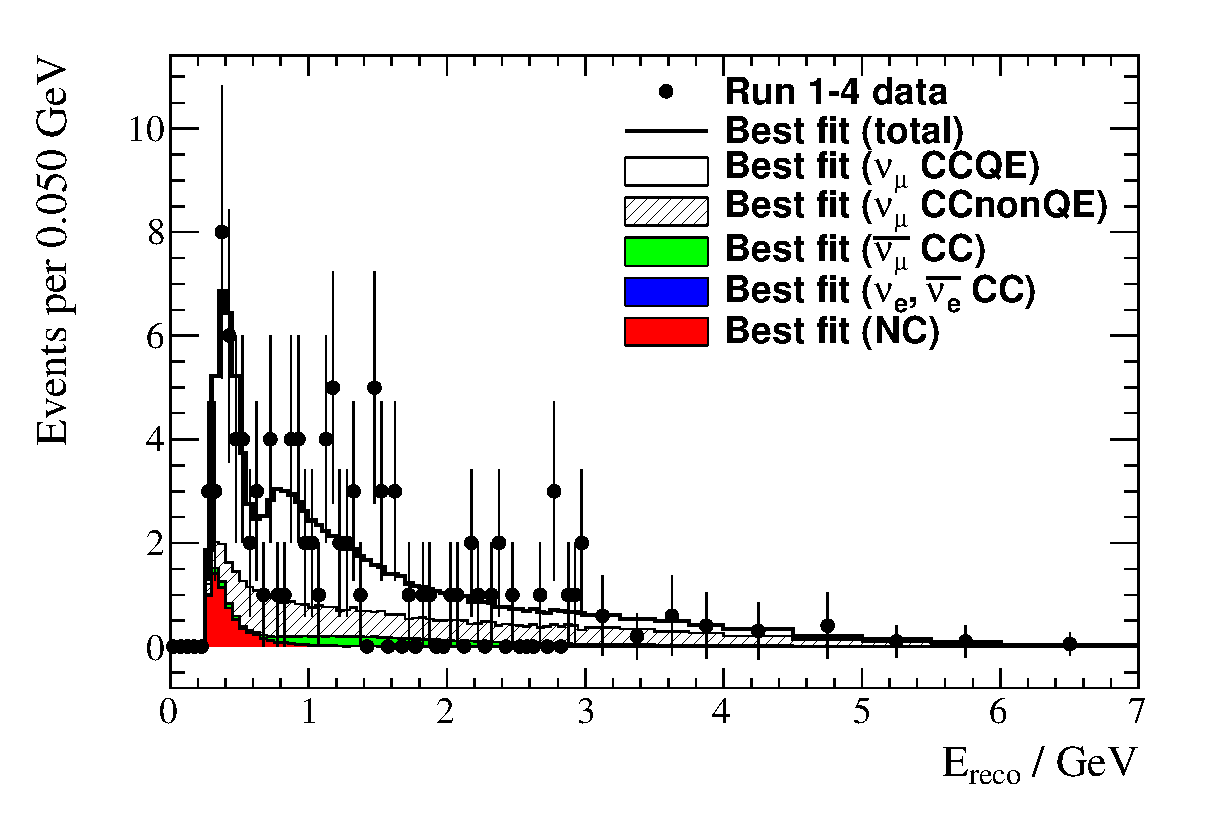
\includegraphics[width=28pc]{./images/data_fit/inverted31/run1-4_nuis4_sintheta_inverted31_spectrumper50_components}
  \caption {
    Best-fit reconstructed energy spectrum in the 73-bin scheme used in the fit (see Sec.\ \ref{sec:mc_templates:template_binning}))
    and its components
    obtained from the fit of the Run 1+2+3+4 dataset.  
    The 32 components, each of which is calculated separately in the analysis, are grouped into just 5 categories:
    $\nu_{\mu}$ CCQE, $\nu_{\mu}$ CCnQE, $\bar{\nu_{\mu}}$ CC, $\nu_{e}$/$\bar{\nu_{e}}$ CC and NC.  
    The inverted mass hierarchy is assumed.
  }
  \label{fig:results_data1234_spectrum_components:inverted}
\end{figure*}


%...........................................................
%
% Best-fit spectra comparisons between normal & inverted hierarchy (73 bin and coarse binning)
%
\begin{figure*}[htb]
\center
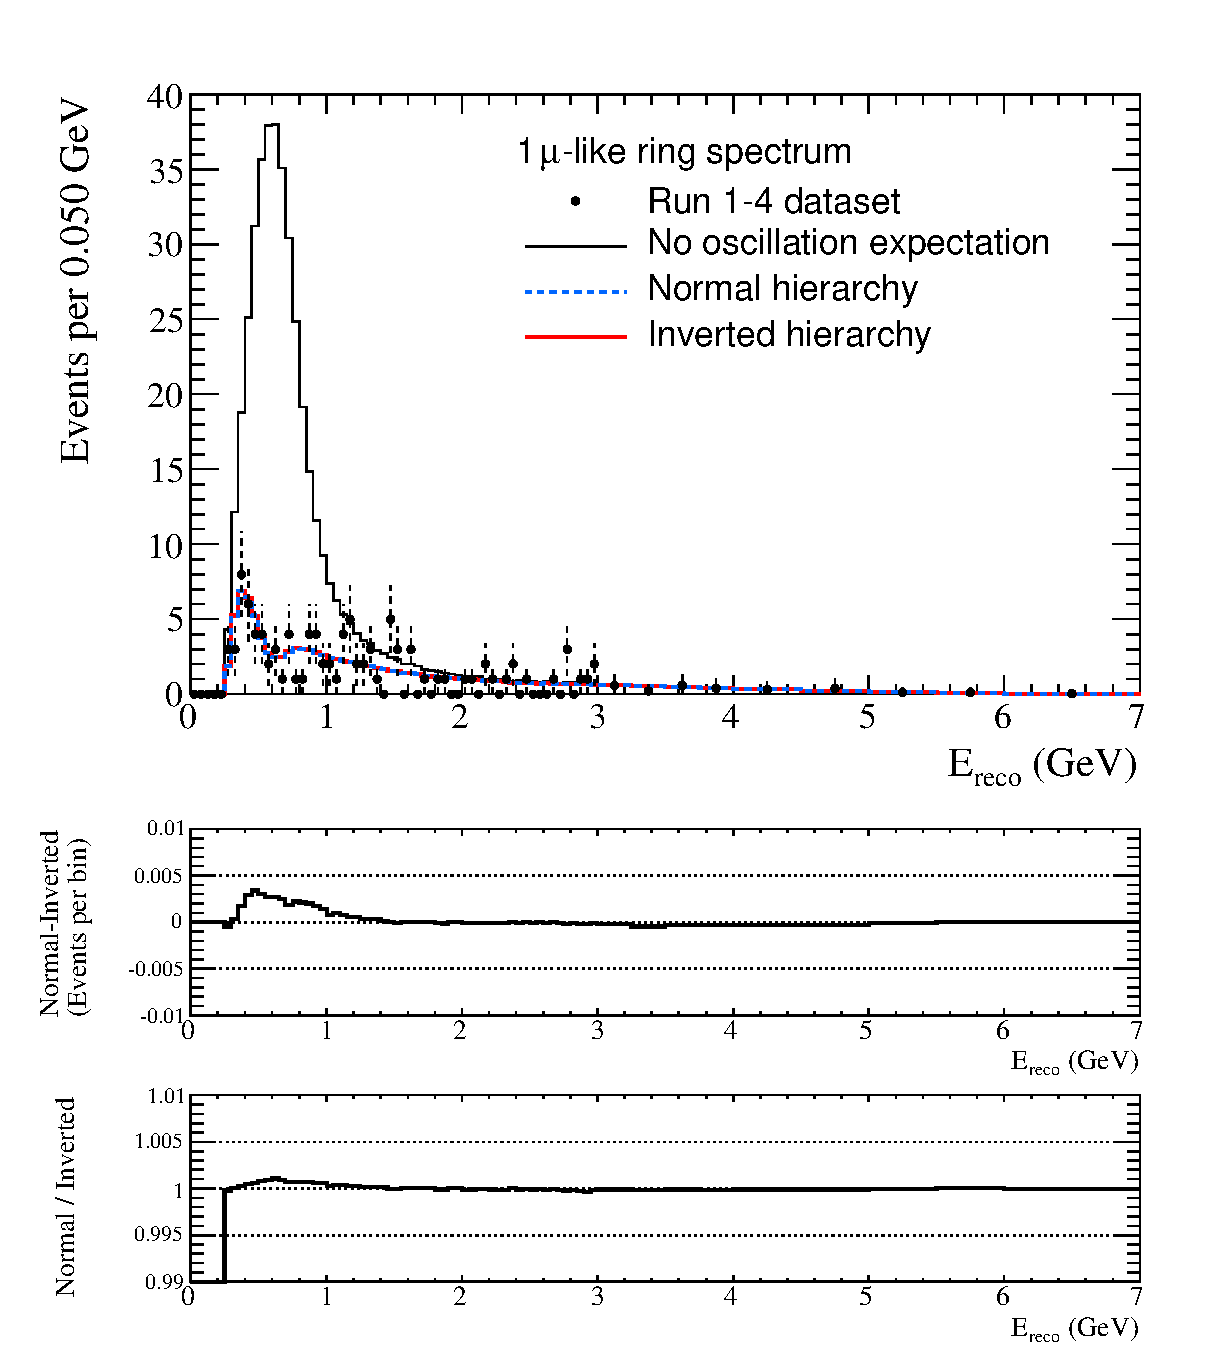
\includegraphics[width=40pc]{./images/data_fit/compare/spectrum_comparison_normal_inverted}
\caption {
  Comparison between best-fit reconstructed energy spectra
  obtained from the normal and inverted mass hierarchy fits of the Run 1+2+3+4 dataset.
  The spectra are shown using the 73 bins used in the fit (see Sec.\ \ref{sec:mc_templates:template_binning}).
  Also shown are the absolute difference between the normal and inverted mass hierarchy
  best-fit predicted spectra and the ratio between them.
}
\label{fig:results_data1234_spectrum_comparison}
\end{figure*}

\begin{figure*}[htb]
\center
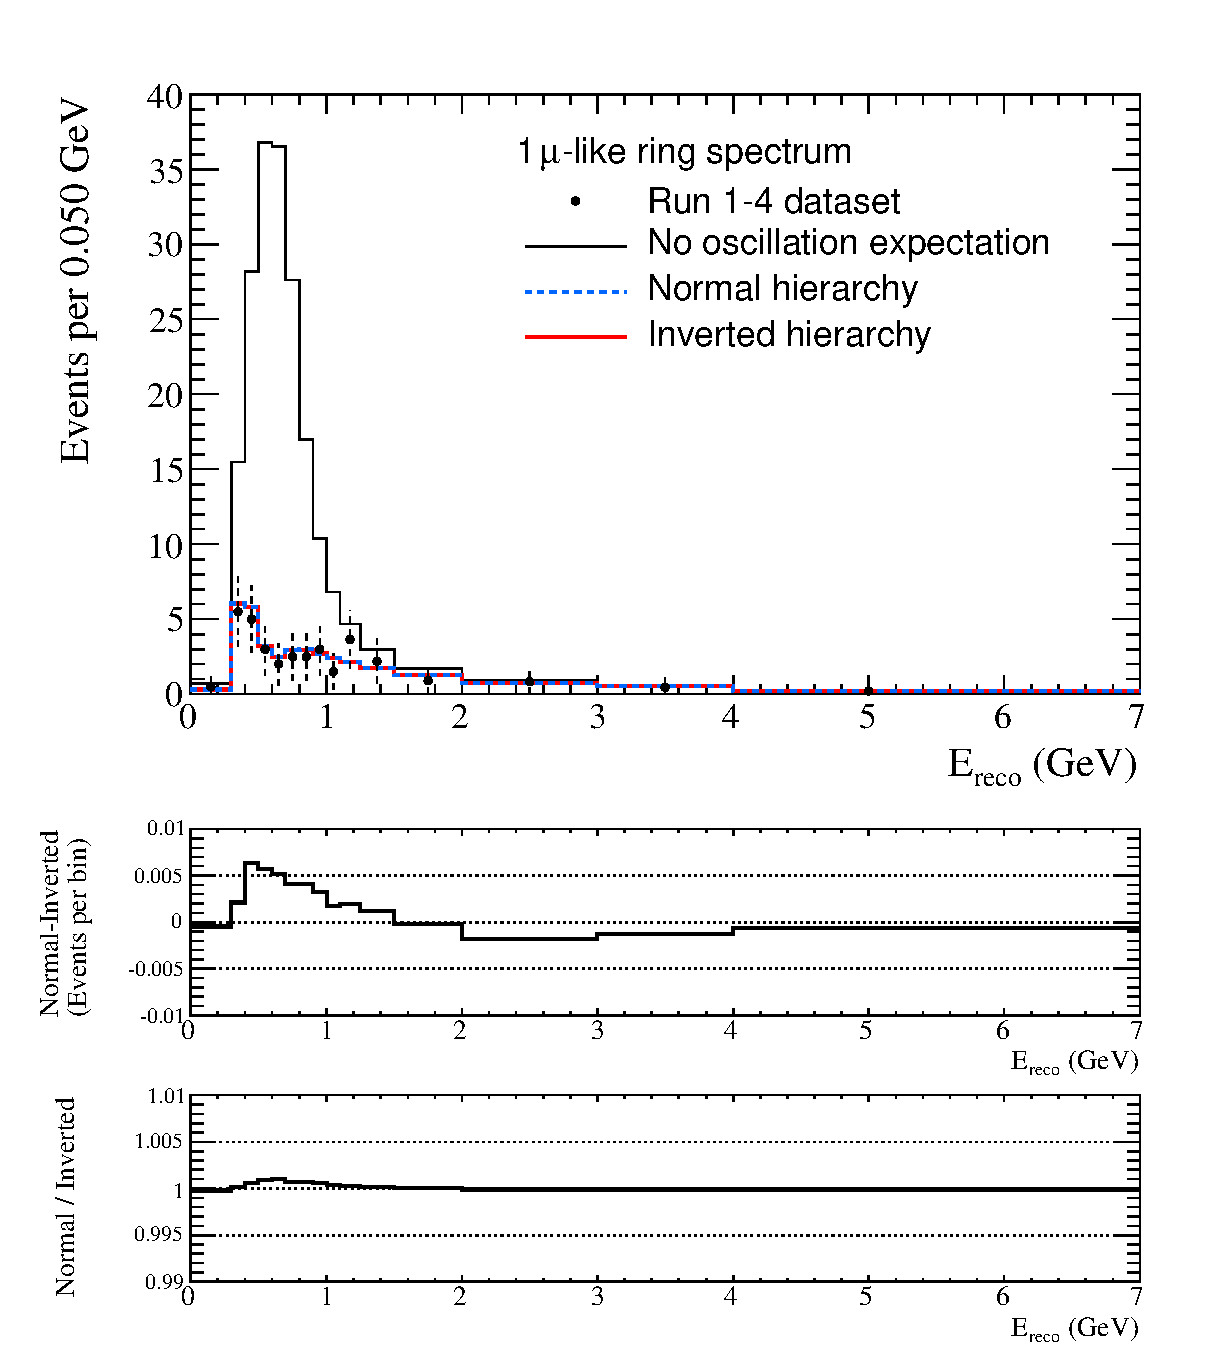
\includegraphics[width=40pc]{./images/data_fit/compare/spectrum_comparison_normal_inverted_coarse}
\caption {
  Comparison between best-fit reconstructed energy spectra
  obtained from the normal and inverted mass hierarchy fits of the Run 1+2+3+4 dataset.
  The spectra are shown using the coarse binning scheme described in Sec.\ \ref{sec:results_bestfit_spectra}.
  Also shown are the absolute difference between the normal and inverted mass hierarchy
  best-fit spectra and the ratio between them.
}
\label{fig:results_data1234_spectrum_comparison_coarse}
\end{figure*}



%...........................................................
%
% Best-fit spectra comparisons between normal run 1+2+3, 4, 1+2+3+4 (73 bin and coarse binning)
%
\begin{figure*}[htb]
\center
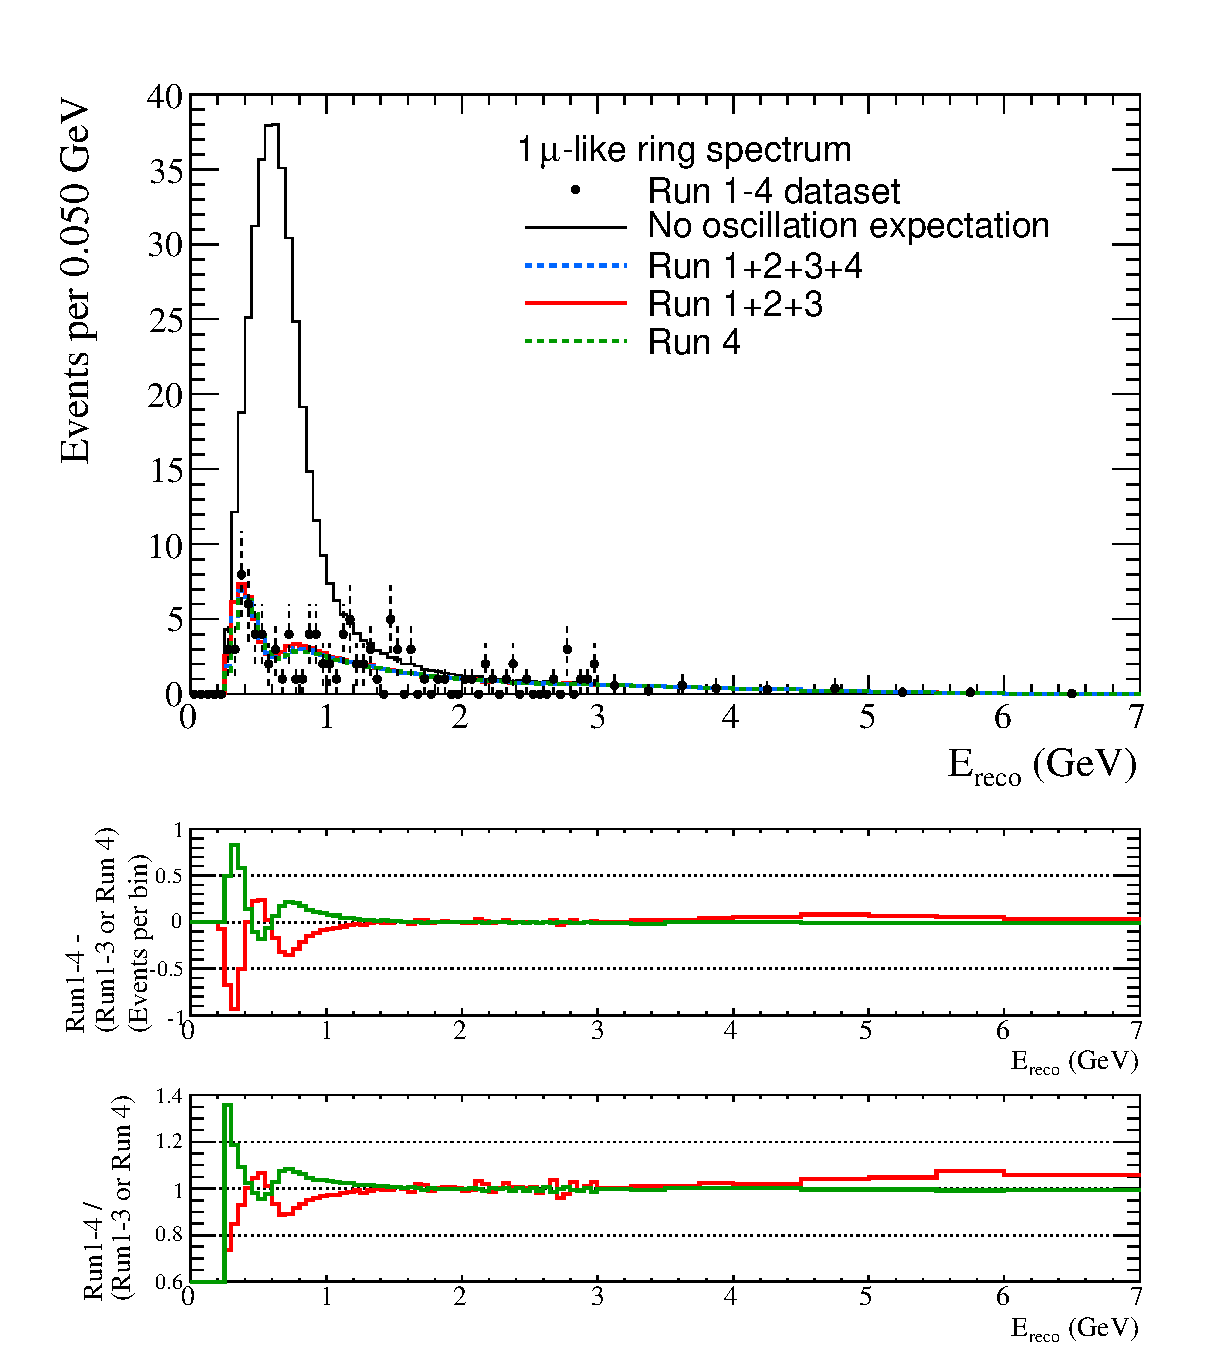
\includegraphics[width=40pc]{./images/data_fit/compare/spectrum_comparison_sepruns}
\caption {
  Comparison between best-fit reconstructed energy spectra
  obtained from the fits to the Run 1+2+3, Run 4, and Run 1+2+3+4 datasets, all scaled to the Run 1+2+3+4 POT,
  for the normal mass hierarchy.
  The spectra are shown using the 73 bins used in the fit (see Sec.\ \ref{sec:mc_templates:template_binning}).
  Also shown are the absolute difference between the scaled Run 1+2+3 or Run 4 best-fit predicted spectra and 
  the Run 1+2+3+4 spectrum and the ratio between them.
}
\label{fig:results_dataruns_spectrum_comparison}
\end{figure*}

\begin{figure*}[htb]
\center
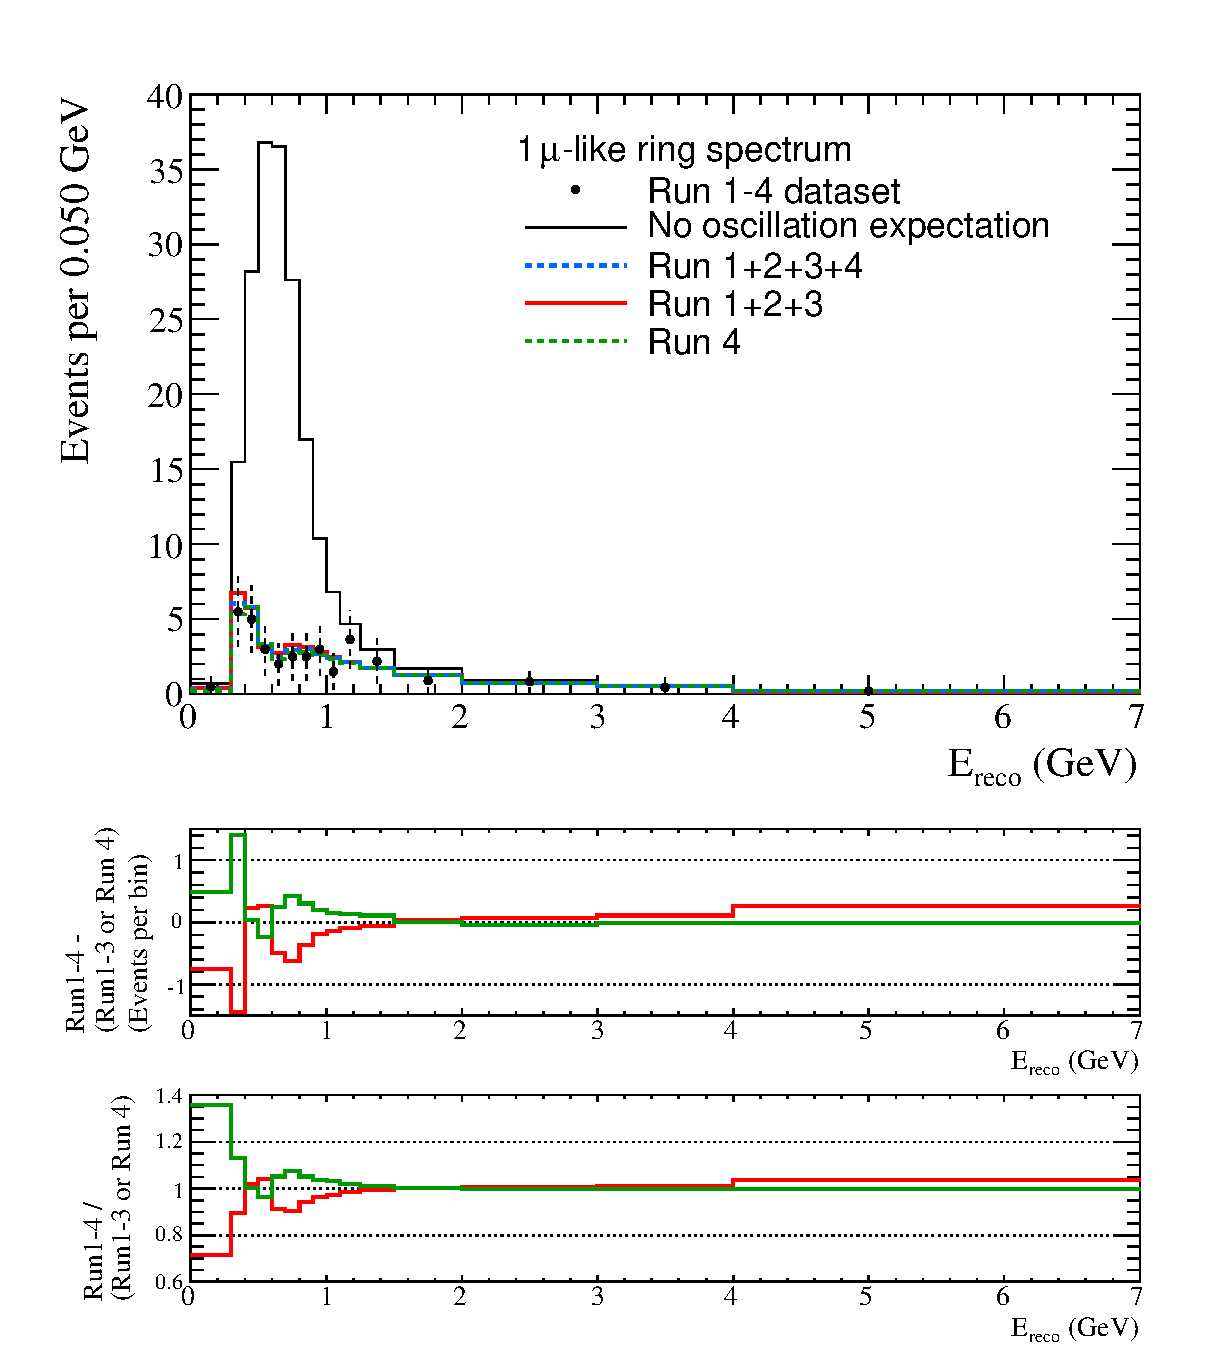
\includegraphics[width=40pc]{./images/data_fit/compare/spectrum_comparison_sepruns_coarse}
\caption {
  Comparison between best-fit reconstructed energy spectra
  obtained from the fits to the Run 1+2+3, Run 4, and Run 1+2+3+4 datasets, all scaled to the Run 1+2+3+4 POT,
  for the normal mass hierarchy.
  The spectra are shown using the coarse binning scheme described in Sec.\ \ref{sec:results_bestfit_spectra}.
  Also shown are the absolute difference between the scaled Run 1+2+3 or Run 4 best-fit predicted spectra and 
  the Run 1+2+3+4 spectrum and the ratio between them.
}
\label{fig:results_dataruns_spectrum_comparison_coarse}
\end{figure*}

%--------------------------------------------------------------------------------------
% Contours
%--------------------------------------------------------------------------------------

\clearpage

\subsection {Confidence regions}
\label{sec:results_contours}

The first step in constructing confidence contours in the 2-dimensional $\sin^{2}\theta_{23}$ - $|\Delta m^{2}_{32}|$ or 
$\sin^{2}\theta_{23}$ - $|\Delta m^{2}_{31}|$
oscillation parameter space is to construct the $\Delta\chi^2$ surface from the fit of the data.
The oscillation parameter space is divided into a rectangular grid of width $\sin^{2}\theta_{23}$ = 0.0025, $|\Delta m^{2}_{32}|$ 
or $|\Delta m^{2}_{31}|$ = 0.025$\times$10$^{-3}$ eV$^{2}$/c$^{4}$, with a grid point at the centre of each rectangle. For each 
mass hierarchy, two separate fits are made of 
the data at each grid point: in one fit, the values of $\sin^{2}\theta_{23}$ and $|\Delta m^{2}_{32}|$ or $|\Delta m^{2}_{31}|$ 
are fixed to the true values of the grid point and the 41 systematic and four non-23 oscillation parameters are allowed to float, 
while, in the other fit, $\sin^{2}\theta_{23}$, $|\Delta m^{2}_{32}|$ or $|\Delta m^{2}_{31}|$,  and the systematic and non-23 
oscillation parameters are allowed to float. $\Delta\chi^2$ is then calculated as the 
difference between the minimum values of $\chi^{2}$ from the two fits ($\chi^{2}$ is defined in Eq.\
\ref{eq:chisquare} in Sec.\ \ref{sec:oscfit_method}).

These 2-dimensional $\Delta\chi^2$ surfaces from the fits of the Run 1+2+3+4 dataset are shown in
Figs.\ \ref{fig:results_data1234_chisq:normal} and \ref{fig:results_data1234_chisq:inverted}
as a function of $\sin^{2}\theta_{23}$ and $|\Delta m^{2}_{32}|$ or $|\Delta m^{2}_{31}|$,
for the normal and inverted mass hierarchies respectively.
For comparison, the corresponding $\Delta\chi^2$ surfaces from the fits of the Run 1+2+3 and Run 4
datasets are shown for the normal mass hierarchy 
in Figs.\ \ref{fig:results_data123_chisq} and \ref{fig:results_data4_chisq} respectively.
The same $\Delta\chi^2$ range is used in all colour plots to allow comparison.

Confidence regions were constructed in the 2-dimensional parameter space $\sin^{2}\theta_{23}$ and $|\Delta m^{2}_{32}|$ or $|\Delta m^{2}_{31}|$
using the constant-$\Delta\chi^2$ method described in Sec.\ \ref{sec:contour_construction} from the
fits of the Run 1+2+3+4, Run 1+2+3 and Run 4 datasets.
The 68\% and 90\% CL regions are shown
in Figs.\ \ref{fig:results_data1234_contour:normal} and \ref{fig:results_data1234_contour:inverted}
for the normal and inverted mass hierarchies respectively.
The corresponding constant-$\Delta\chi^2$ contours for the Run 1+2+3 and Run 4 datasets are shown
in Figs.\ \ref{fig:results_data123_contour} and \ref{fig:results_data4_contour} respectively.

To construct 2-dimensional confidence regions using the method of Feldman and Cousins \cite{FeldmanCousins},
the $\Delta\chi^{2}_{critical}$ surfaces must be calculated in the $\sin^{2}\theta_{23}$ - $|\Delta m^{2}_{32}|$
or $\sin^{2}\theta_{23}$ - $|\Delta m^{2}_{31}|$ oscillation parameter space as described in Sec.\ \ref{sec:contour_construction}.
In Figs.\ \ref{fig:fc_dchisqcrit_2d:normal} and \ref{fig:fc_dchisqcrit_2d:inverted}, we show a Monte Carlo estimation
of the 2-dimensional Feldman-Cousins $\Delta\chi^{2}_{critical}$ values
used for calculation of the 68\% and 90\% CL confidence regions for the normal mass hierarchy and inverted mass hierarchy respectively.
These $\Delta\chi^{2}_{critical}$ surfaces were generated using an ensemble of toy MC experiments which included both
randomized systematic variations and statistical fluctuations.
One-dimensional slices of these $\Delta\chi^{2}_{critical}$ surfaces
are shown in Figs.\ \ref{fig:fc_dchisqcrit_slice_mixing:normal} and \ref{fig:fc_dchisqcrit_slice_dmsq:normal} for the normal mass hierarchy,
and in Figs.\ \ref{fig:fc_dchisqcrit_slice_mixing:inverted} and \ref{fig:fc_dchisqcrit_slice_dmsq:inverted} for the inverted mass hierarchy.
The Feldman-Cousins values of $\Delta\chi^{2}_{critical}$ are lower than the canonical constant-$\Delta\chi^{2}_{critical}$ values
when the true input value of $\sin^2 \theta_{23}$ is near the value of maximal $\nu_{\mu}$ disappearance. 
Under these circumstances, the best-fit values of $\sin^2 \theta_{23}$ pile up at the value of maximal disappearance, and this gives lower
values of $\Delta\chi^{2}$ than would be obtained if that boundary did not exist. Consequently, the 68\% and 90\% critical $\Delta\chi^{2}$
values are lower than the canonical constant-$\Delta\chi^{2}$ values.

Using the $\Delta\chi^2$ and $\Delta\chi^{2}_{critical}$ surfaces presented here,
the 2-dimensional Feldman-Cousins 68\% and 90\% CL regions were constructed
and they are shown in Figs.\ \ref{fig:results_data1234_fc_contour:normal} and
\ref{fig:results_data1234_fc_contour:inverted}.

Profile $\Delta\chi^2$ distributions were also calculated from the 2-dimensional $\Delta\chi^2$ surfaces, and are shown as a 
function of $\sin^{2}\theta_{23}$ and $|\Delta m^{2}_{32}|$ or $|\Delta m^{2}_{31}|$ from the
fits of the Run 1+2+3+4 dataset in 
Figs.\ \ref{fig:results_marg_dchisq_dmsq_normalinverted} and \ref{fig:results_marg_dchisq_sinsq_normalinverted} respectively.
These profile $\Delta\chi^2$ distributions are compared with those from the fits of the Run 1+2+3 and Run 4 datasets for the normal 
mass hierarchy in Figs.\ \ref{fig:results_marg_dchisq_dmsq_all3} and \ref{fig:results_marg_dchisq_sinsq_all3}
for $\sin^{2}\theta_{23}$ and $|\Delta m^{2}_{32}|$ respectively.
Using these plots and the constant-$\Delta\chi^2$ method described in Sec.\ \ref{sec:contour_construction},
1-dimensional limits on the parameters can be obtained for each parameter separately\footnote{
For 1 fit parameter, the critical values of $\Delta{\chi^{2}}$ used are 
1.00 (68\% CL), 2.71 (90\% CL), 3.84 (95\% CL), 6.63 (99\% CL).
For 2 parameters fitted simultaneously, the critical values of $\Delta{\chi^{2}}$ used are 
2.30 (68\% CL), 4.61 (90\% CL), 5.99 (95\% CL), 9.21 (99\% CL).
}.
These limits are presented in Tab.\ \ref{tab:data_fits:1dlimits}.

1-dimensional confidence intervals were also constructed separately for each of $\sin^2 \theta_{23}$ and $|\Delta m_{32}^{2}|$ (normal mass hierarchy) 
or $|\Delta m_{31}^{2}|$ (inverted mass hierarchy) using the new procedure described in Sec.\ \ref{sec:contour_construction}. For the normal 
mass hierarchy, a Monte Carlo estimation of the 68\% and 90\% 1D critical $\Delta\chi^{2}$ values for $\sin^2 \theta_{23}$ was made using 
10000 toy experiments with systematic variations and statistical fluctuations at each value of that parameter, with the input values of 
$|\Delta m_{32}^{2}|$ being chosen using the method described in Sec.\ \ref{sec:contour_construction}. These critical $\Delta\chi^{2}$ values are shown in 
Fig.\ \ref{fig:results_1D_dchisq_sinsq_normal}, in which they are fitted with cubic splines. The 68\% and 90\% confidence intervals in 
$\sin^2 \theta_{23}$ include the values of that parameter for which $\Delta\chi^{2}$ from the 1D fit of the Run 1+2+3+4 data is less than the 
appropriate MC critical values. In practice, this was done by finding the values of $\sin^2 \theta_{23}$ where the cubic splines intersect the 
plot of the 1D $\Delta\chi^{2}$ from the fit of the data (see Fig.\ \ref{fig:results_1D_dchisq_sinsq_normal}). The 68\% and 90\% confidence 
intervals in $|\Delta m_{32}^{2}|$ were constructed in a similar way, and the MC critical $\Delta\chi^{2}$ values and the 1D $\Delta\chi^{2}$ 
from the fit of the data are shown in Fig.\ \ref{fig:results_1D_dchisq_dm32sq_normal}. 

In Fig.\ \ref{fig:results_1D_dchisq_sinsq_normal}, it is apparent that the MC critical $\Delta\chi^{2}$ values are lower than the canonical 
constant-$\Delta\chi^{2}$ values when the true input value of $\sin^2 \theta_{23}$ is near the value of maximal $\nu_{\mu}$ disappearance. 
Again this is due to the best-fit values of $\sin^2 \theta_{23}$ in the toy MC experiments piling up at the value of maximal disappearance.
At input values of $\sin^2 \theta_{23}$ far from the value of maximal 
$\nu_{\mu}$ disappearance, the critical $\Delta\chi^{2}$ values approach the canonical constant-$\Delta\chi^{2}$ values as expected. The MC 
critical $\Delta\chi^{2}$ values for $|\Delta m_{32}^{2}|$ are lower than the canonical constant-$\Delta\chi^{2}$ values for all input values 
of that parameter. This is due to the input values of $\sin^2 \theta_{23}$ to the toy experiments, many of which are near the value of maximal 
$\nu_{\mu}$ disappearance (see Fig.\ \ref{fig:input_mixing23_1DFC} for an example). Again the best-fit values of $\sin^2 \theta_{23}$ pile up 
at the value of maximal disappearance, which results in lower values of $\Delta\chi^{2}$ than would occur if that boundary were not present. 

For the inverted mass hierarchy, the Monte Carlo estimations of the 68\% and 90\% 1D critical $\Delta\chi^{2}$ values for $\sin^2 \theta_{23}$ 
were made using input values of $|\Delta m_{31}^{2}|$ that were chosen according to the method described in Sec.\ \ref{sec:contour_construction}. 
These critical $\Delta\chi^{2}$ values are compared with the $\Delta\chi^{2}$ from the 1D fits of the Run 1+2+3+4 data in Figs.\ 
\ref{fig:results_1D_dchisq_sinsq_inverted} and \ref{fig:results_1D_dchisq_dm32sq_inverted}; the results show a similar pattern to those for 
the normal mass hierarchy.

The 68\% and 90\% confidence intervals from the new procedure in $\sin^2 \theta_{23}$ and $|\Delta m_{32}^{2}|$ (normal mass hierarchy) or 
$|\Delta m_{31}^{2}|$ (inverted mass hierarchy) are given in Tab.\ \ref{tab:data_fits:1dlimits}. They clearly show that the confidence 
intervals from the constant-$\Delta\chi^{2}$ method overcover for both $\sin^2 \theta_{23}$ and the mass-squared difference; this overcoverage 
is caused by the boundary effects from the value of maximial disappearance  in $\sin^2 \theta_{23}$.

In the next section, comparisons are presented of the confidence regions obtained 
using different construction methods.
The contours from different running periods are compared, and we also compare our contours
from the fit to the combined Run 1+2+3+4 dataset with recent measurements from MINOS and 
SuperK and T2K 6.5700$\times$10$^{20}$-POT sensitivity contours. 


%...........................................................
%
% \Delta\chisquare surfaces 
%
\begin{figure*}[htb]
  \begin{minipage}[t]{0.96\linewidth}
    \center
    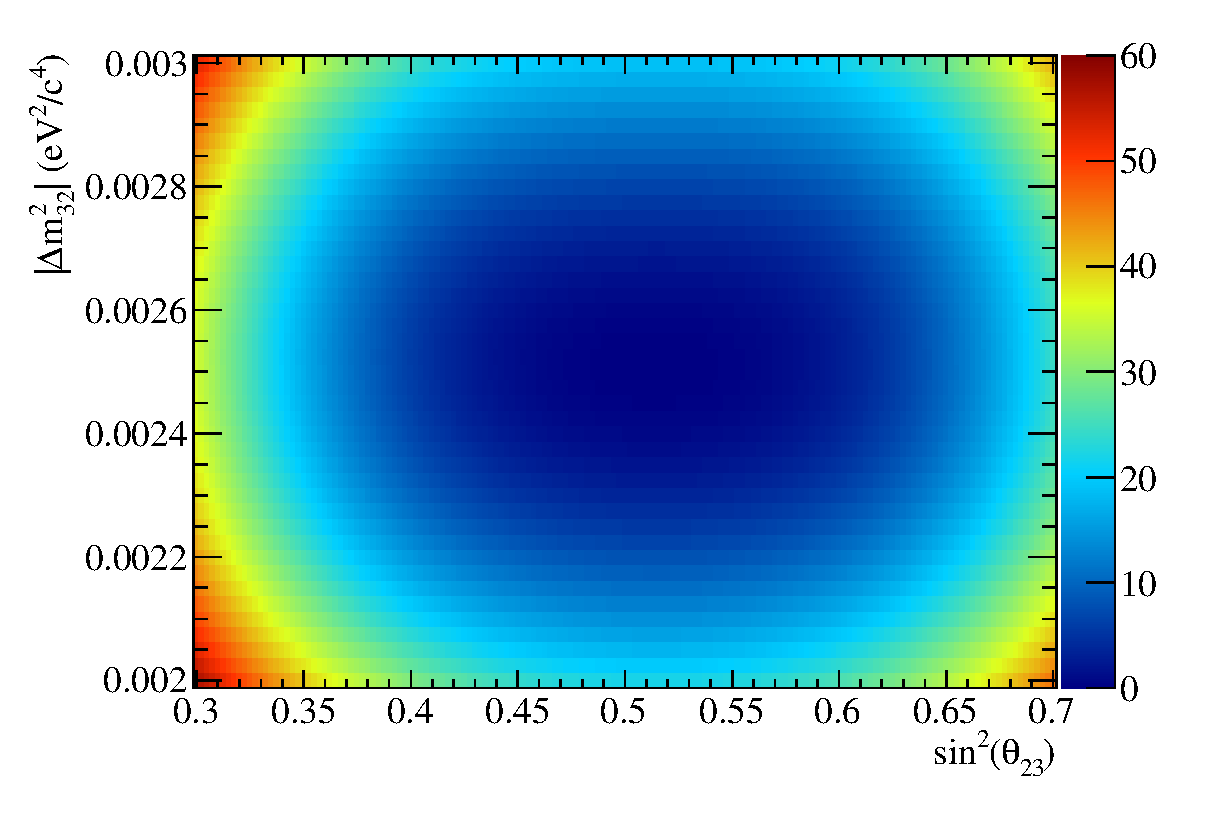
\includegraphics[width=36pc]{./images/data_fit/normal/run1-4_nuis4_sintheta_normal_dchisq_maxz60}
    \caption {
      $\Delta\chi^2$ surface from the fit of the Run 1+2+3+4 dataset.
      The normal mass hierarchy is assumed.
    }
    \label{fig:results_data1234_chisq:normal}
  \end{minipage}
  \vfill
  \begin{minipage}[t]{0.96\linewidth}
    \center
    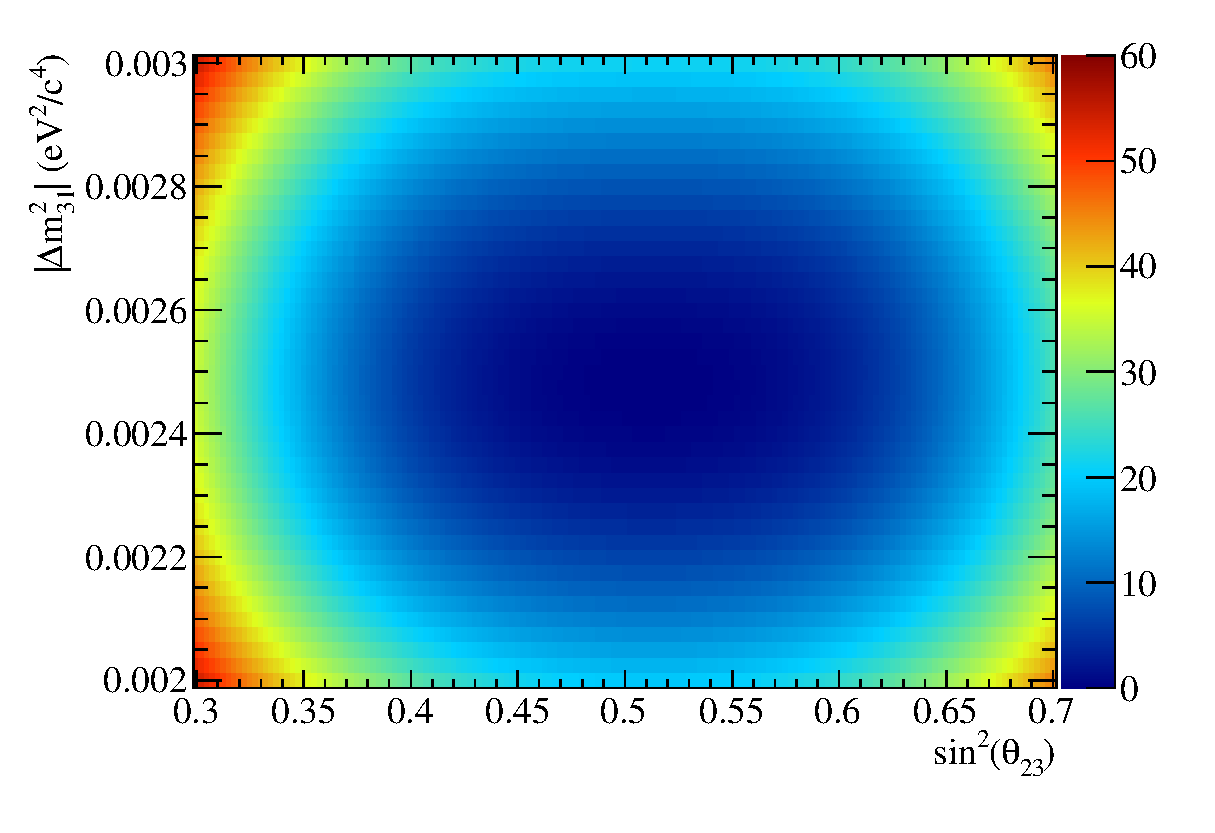
\includegraphics[width=36pc]{./images/data_fit/inverted31/run1-4_nuis4_sintheta_inverted31_dchisq_maxz60}
    \caption {
      $\Delta\chi^2$ surface from the fit of the Run 1+2+3+4 dataset.
      The inverted mass hierarchy is assumed.
    }
    \label{fig:results_data1234_chisq:inverted}
  \end{minipage}
\end{figure*}


\begin{figure*}[htb]
\begin{minipage}[t]{0.48\linewidth}
\center
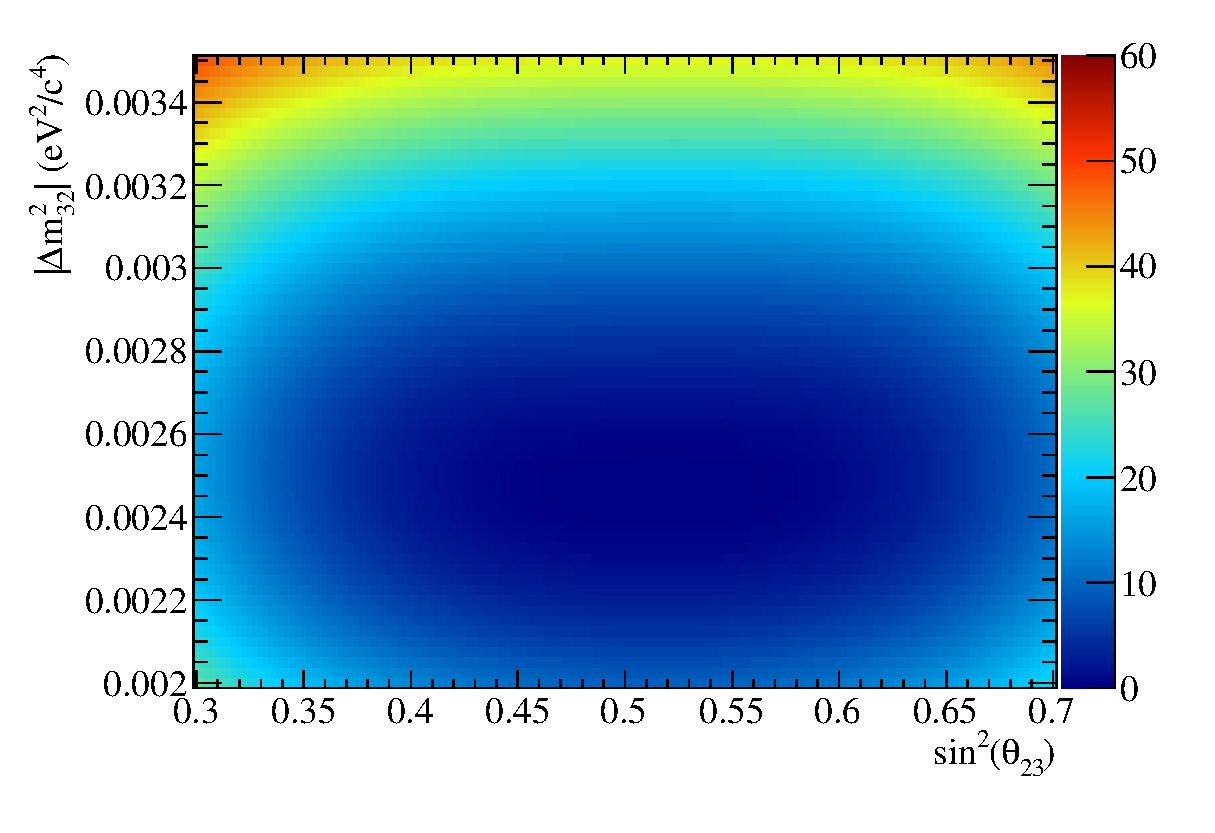
\includegraphics[width=21pc]{./images/data_fit/run123/run1-4_nuis4_sintheta_normal_run123_dchisq_maxz60}
\caption {
  $\Delta\chi^2$ surface from the fit of the Run 1+2+3 dataset.
  The normal mass hierarchy is assumed.
}
\label{fig:results_data123_chisq}
\end{minipage}
\hspace{0.06\linewidth}
\begin{minipage}[t]{0.48\linewidth}
\center
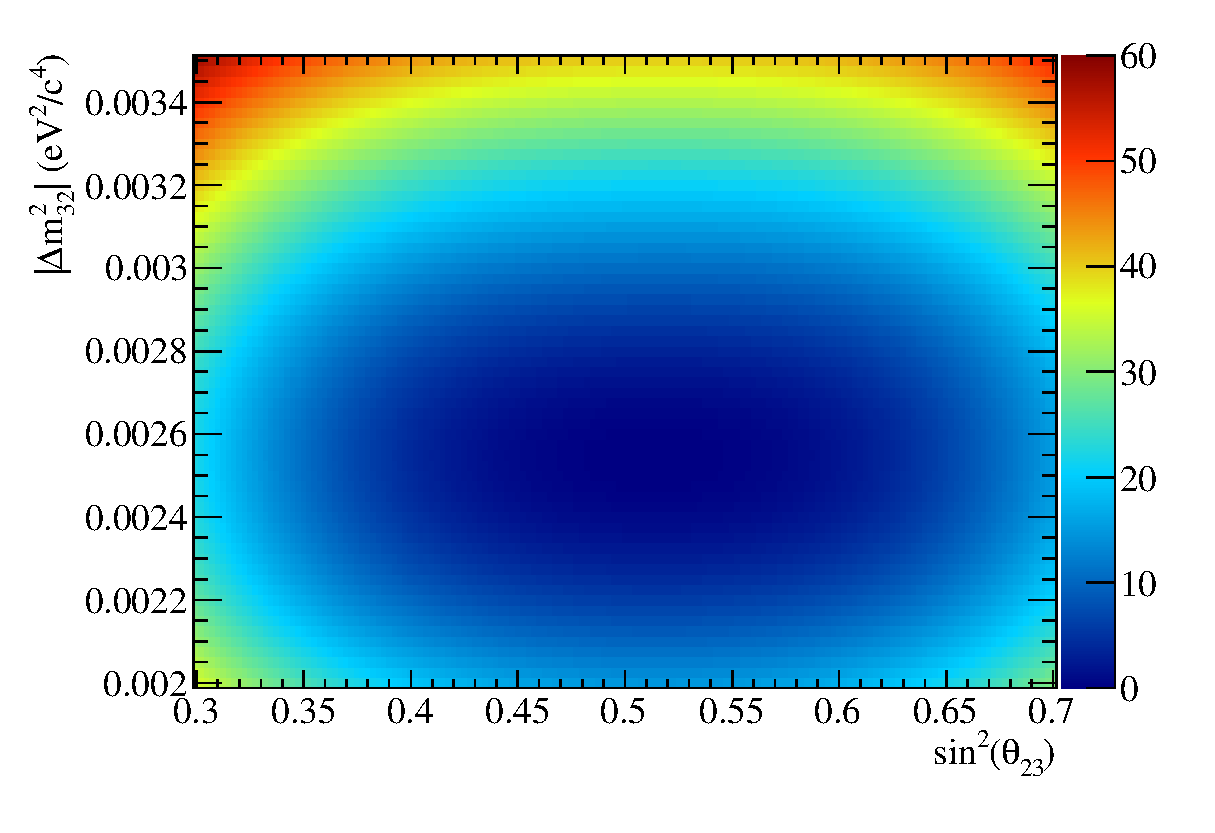
\includegraphics[width=21pc]{./images/data_fit/run4/run1-4_nuis4_sintheta_normal_run4_dchisq_maxz60}
\caption {
  $\Delta\chi^2$ surface from the fit of the Run 4 dataset.
  The normal mass hierarchy is assumed.
}
\label{fig:results_data4_chisq}
\end{minipage}
\end{figure*}

\clearpage

%...........................................................
%
% Const-dchi^2 contours 
%

\clearpage

\begin{figure*}[htb]
\center
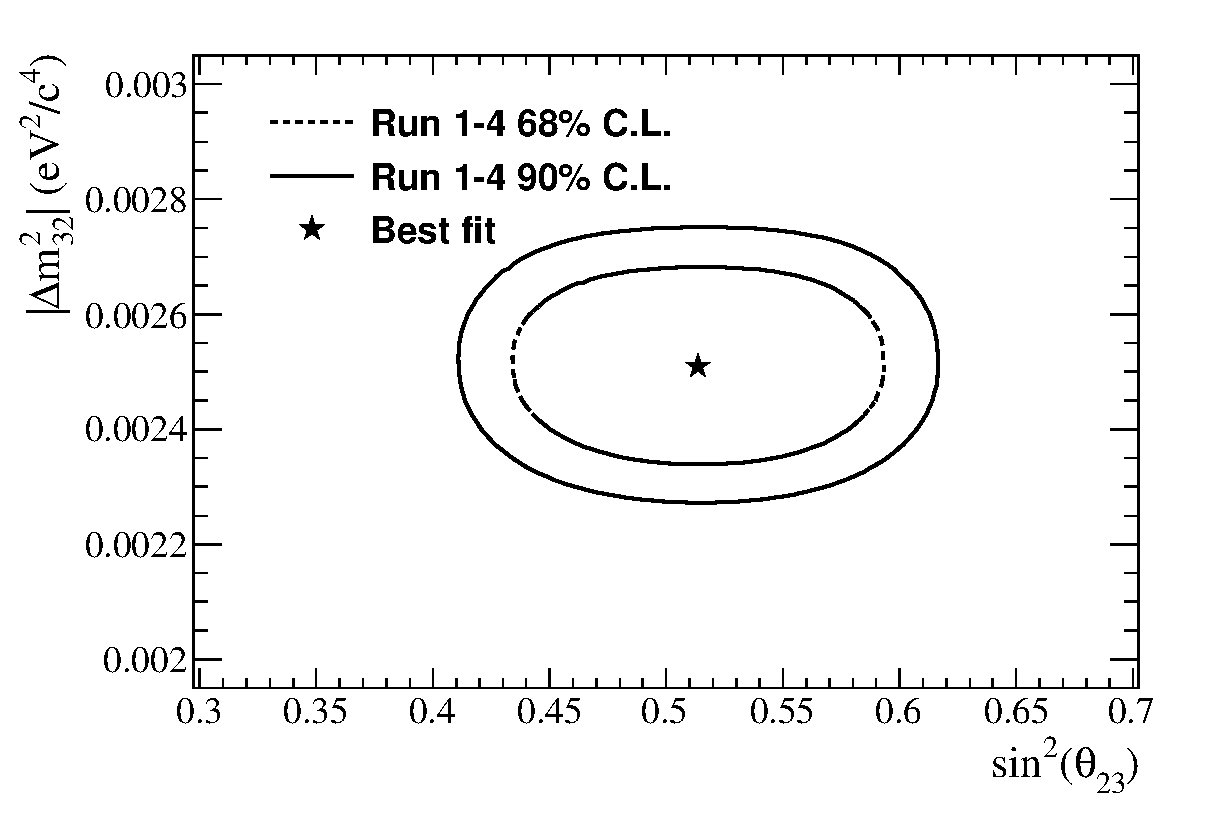
\includegraphics[width=30pc]{./images/data_fit/normal/run1-4_nuis4_sintheta_normal_contour}
\caption {
  68\% CL and 90\% CL allowed regions, 
  constructed with the constant-$\Delta\chi^{2}$ method,
  from the fit of the Run 1+2+3+4 dataset, 
  with the effects of statistical fluctuations and systematic variations being included. 
  The best-fit point is also shown.
  The normal mass hierarchy is assumed.
}
\label{fig:results_data1234_contour:normal}
\end{figure*}

\begin{figure*}[htb]
\center
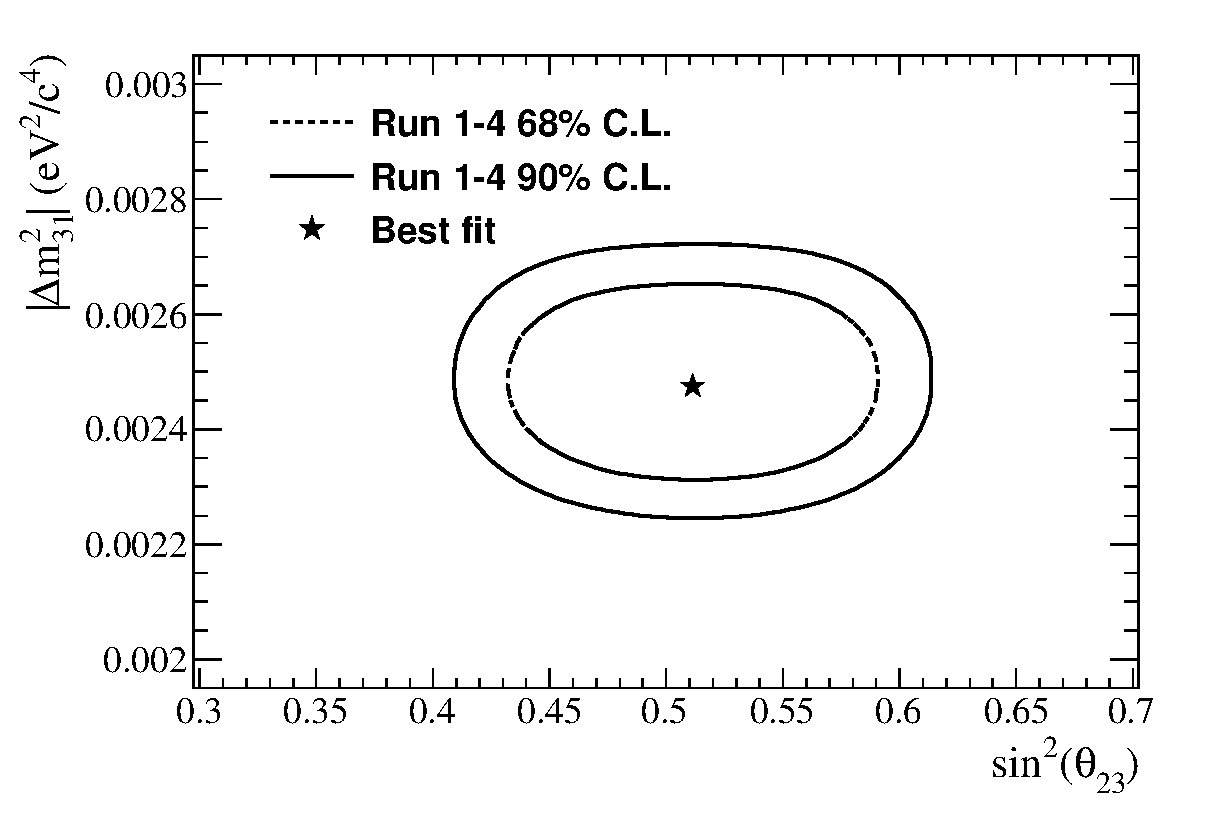
\includegraphics[width=30pc]{./images/data_fit/inverted31/run1-4_nuis4_sintheta_inverted31_contour}
\caption {
  68\% CL and 90\% CL allowed region, 
  constructed with the constant-$\Delta\chi^{2}$ method,
  from the fit of the Run 1+2+3+4 dataset,
  with the effects of statistical fluctuations and systematic variations being included.
  The best-fit point is also shown.
  The inverted mass hierarchy is assumed.
}
\label{fig:results_data1234_contour:inverted}
\end{figure*}

\begin{figure*}[htb]
\begin{minipage}[t]{0.48\linewidth}
\center
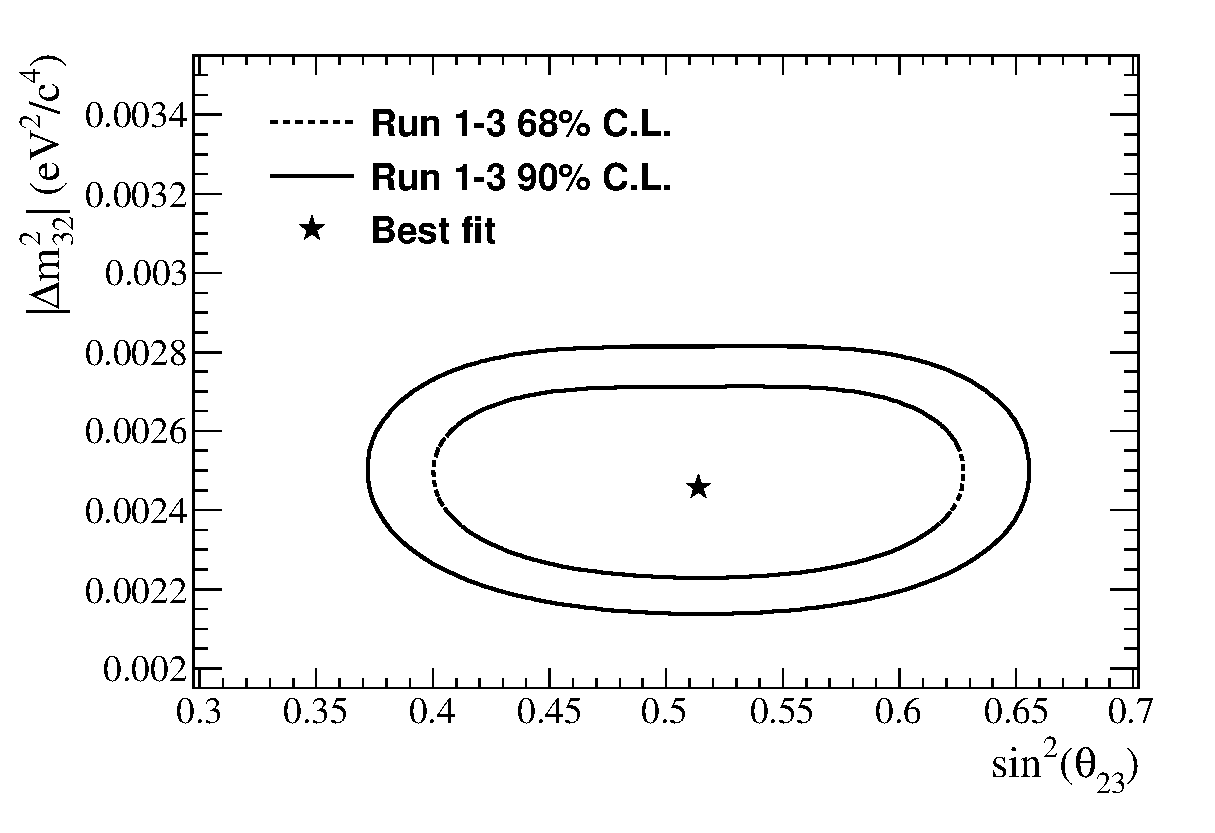
\includegraphics[width=20pc]{./images/data_fit/run123/run1-4_nuis4_sintheta_normal_run123_contour}
\caption {
  68\% CL and 90\% CL allowed regions,
  constructed with the constant-$\Delta\chi^{2}$ method,
  from the fit of the Run 1+2+3 dataset,
  with the effects of statistical fluctuations and systematic variations being included.
  The best-fit point is also shown.
  The normal mass hierarchy is assumed.
}
\label{fig:results_data123_contour}
\end{minipage}
\hspace{0.06\linewidth}
\begin{minipage}[t]{0.48\linewidth}
\center
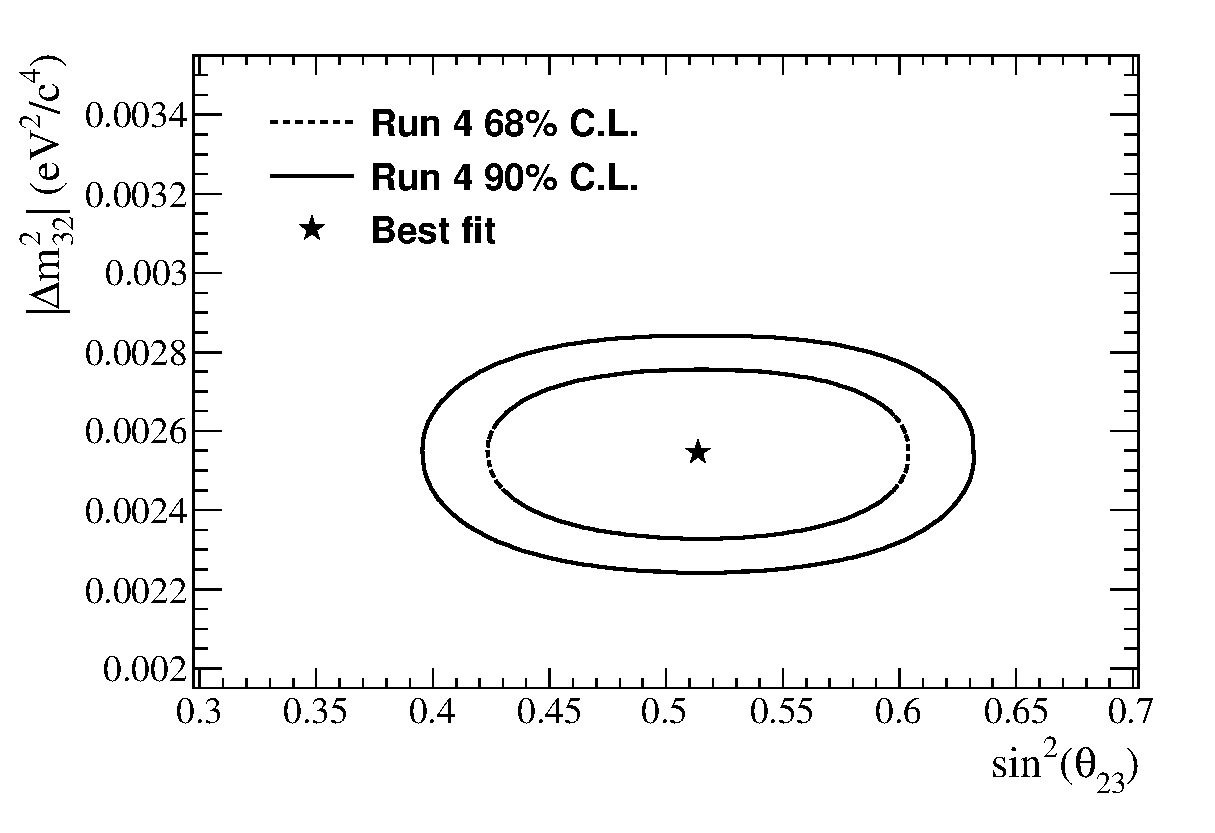
\includegraphics[width=20pc]{./images/data_fit/run4/run1-4_nuis4_sintheta_normal_run4_contour}
\caption {
  68\% CL and 90\% CL allowed regions,
  constructed with the constant-$\Delta\chi^{2}$ method,
  from the fit of the Run 4 dataset only,
  with the effects of statistical fluctuations and systematic variations being included.
  The best-fit point is also shown.
  The normal mass hierarchy is assumed.
}
\label{fig:results_data4_contour}
\end{minipage}
\end{figure*}

%...........................................................
%
% FC dchisq_critical surfaces
% 

\clearpage

\begin{figure*}[htb]
  \center
  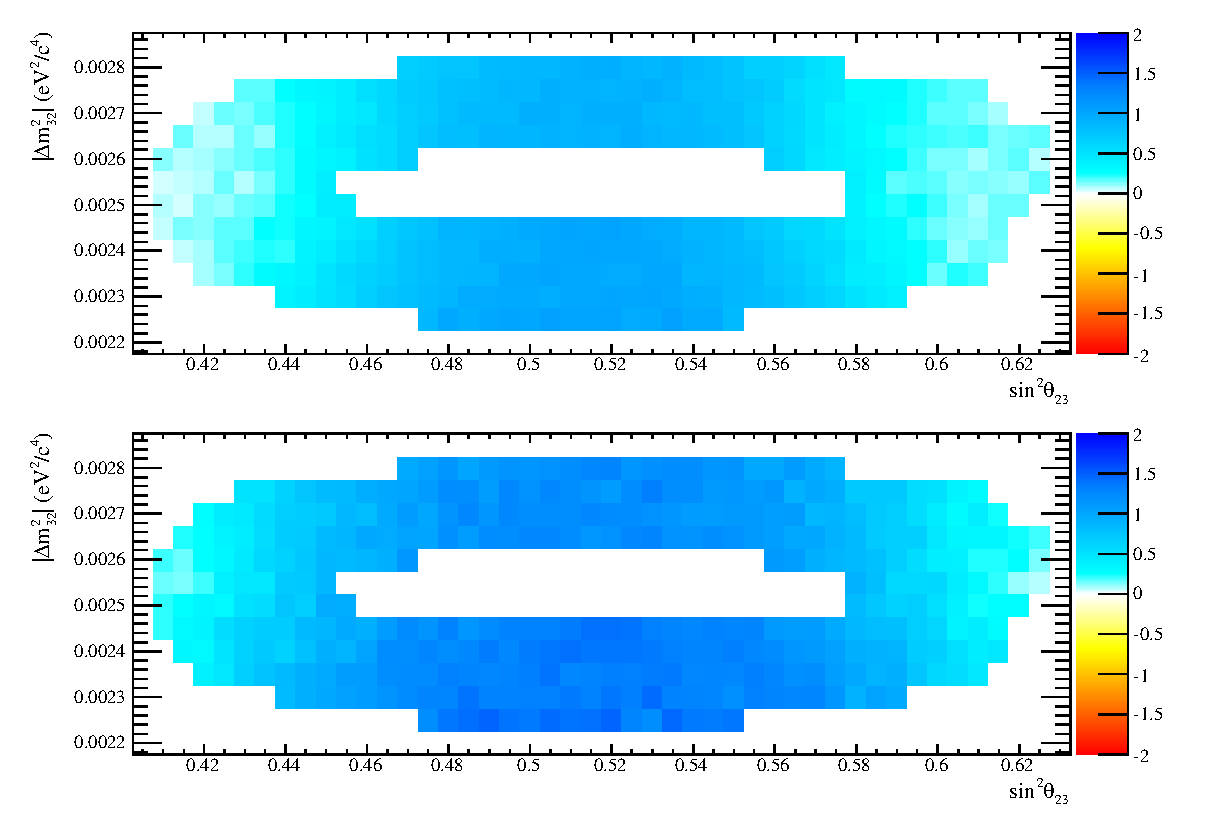
\includegraphics[width=42pc]{./images/fc_surface/FC_surfaces_normal}
  \caption {
    Difference between the $\Delta\chi^2_{critical}$ values obtained from the constant-$\Delta\chi^2$ method 
    and those from the Feldman-Cousins method \cite{FeldmanCousins} at confidence levels of 68\% (top) and 90\% (bottom),
    as a function of $\sin^{2}{\theta_{23}}$ and $|\Delta{m^{2}_{32}}|$.
    These surfaces were generated from an ensemble of toy MC experiments including both
    randomized systematic variations and statistical fluctuations.
    As expected from \cite{FeldmanCousins}, the Feldman-Cousins $\Delta\chi^{2}_{critical}$ values
    decrease as maximal $\nu_{\mu}$ disappearance at $\sin^{2}{\theta_{23}}$ $\approx$ 0.513 is approached.
    The normal mass hierarchy is assumed.
    $\Delta\chi^2_{critical}$ is only calculated for values of 
    $\sin^{2}{\theta_{23}}$ and $|\Delta{m^{2}_{32}}|$
    that affect the 68\% and 90\% confidence contours. 
    }
  \label{fig:fc_dchisqcrit_2d:normal}
\end{figure*}

%.......

\clearpage

\begin{figure*}[htb]
  \center
  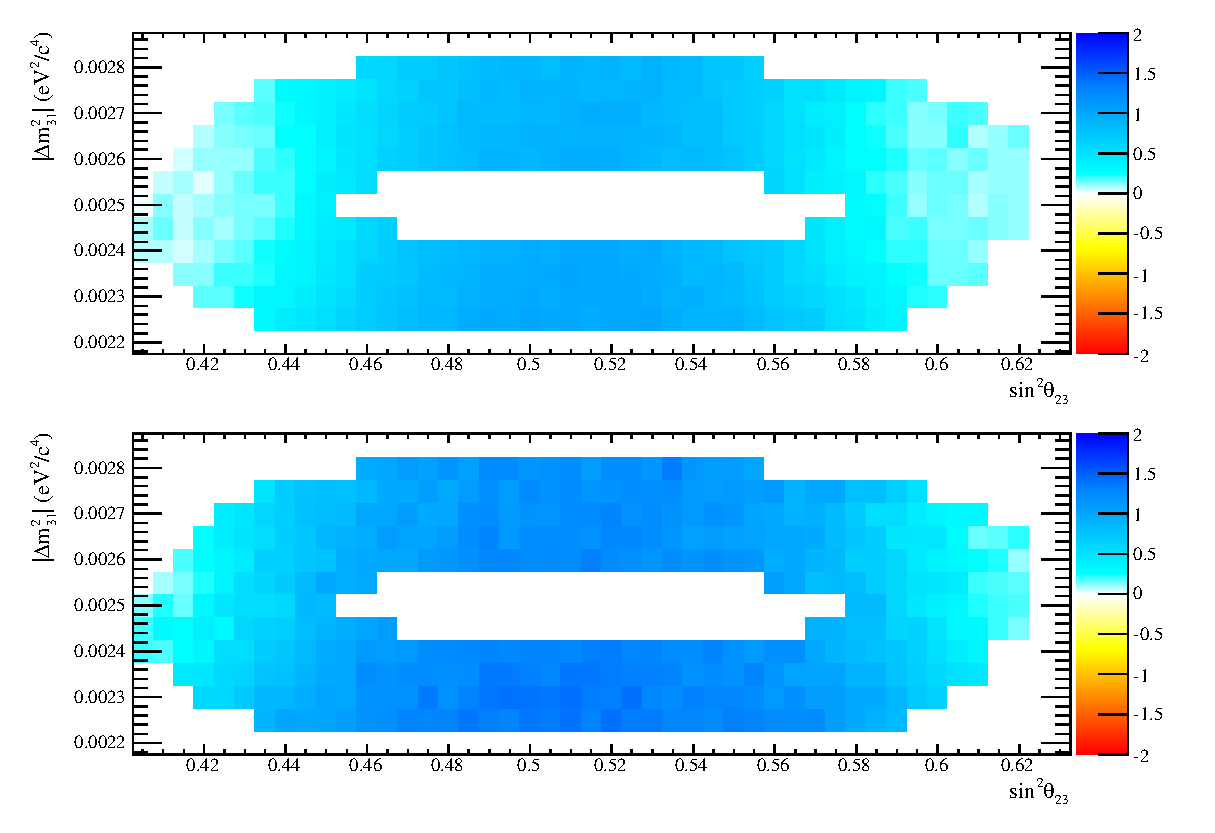
\includegraphics[width=42pc]{./images/fc_surface/FC_surfaces_inverted31}
  \caption {
    Difference between the $\Delta\chi^2_{critical}$ values obtained from the constant-$\Delta\chi^2$ method
    and those from the Feldman-Cousins method \cite{FeldmanCousins} at confidence levels of 68\% (top) and 90\% (bottom),
    as a function of $\sin^{2}{\theta_{23}}$ and $|\Delta{m^{2}_{31}}|$.
    These surfaces were generated from an ensemble of toy MC experiments including both
    randomized systematic variations and statistical fluctuations.
    As expected from \cite{FeldmanCousins}, the Feldman-Cousins $\Delta\chi^{2}_{critical}$ values
    decrease as maximal $\nu_{\mu}$ disappearance at $\sin^{2}{\theta_{23}}$ $\approx$ 0.513 is approached.
    The inverted mass hierarchy is assumed.
    $\Delta\chi^2_{critical}$ is only calculated for values of
    $\sin^{2}{\theta_{23}}$ and $|\Delta{m^{2}_{32}}|$
    that affect the 68\% and 90\% confidence contours.
  }
  \label{fig:fc_dchisqcrit_2d:inverted}
\end{figure*}

%...........................................................
%
% FC dchisq_critical surface projections
% 

\begin{figure*}[htb]
  \center
  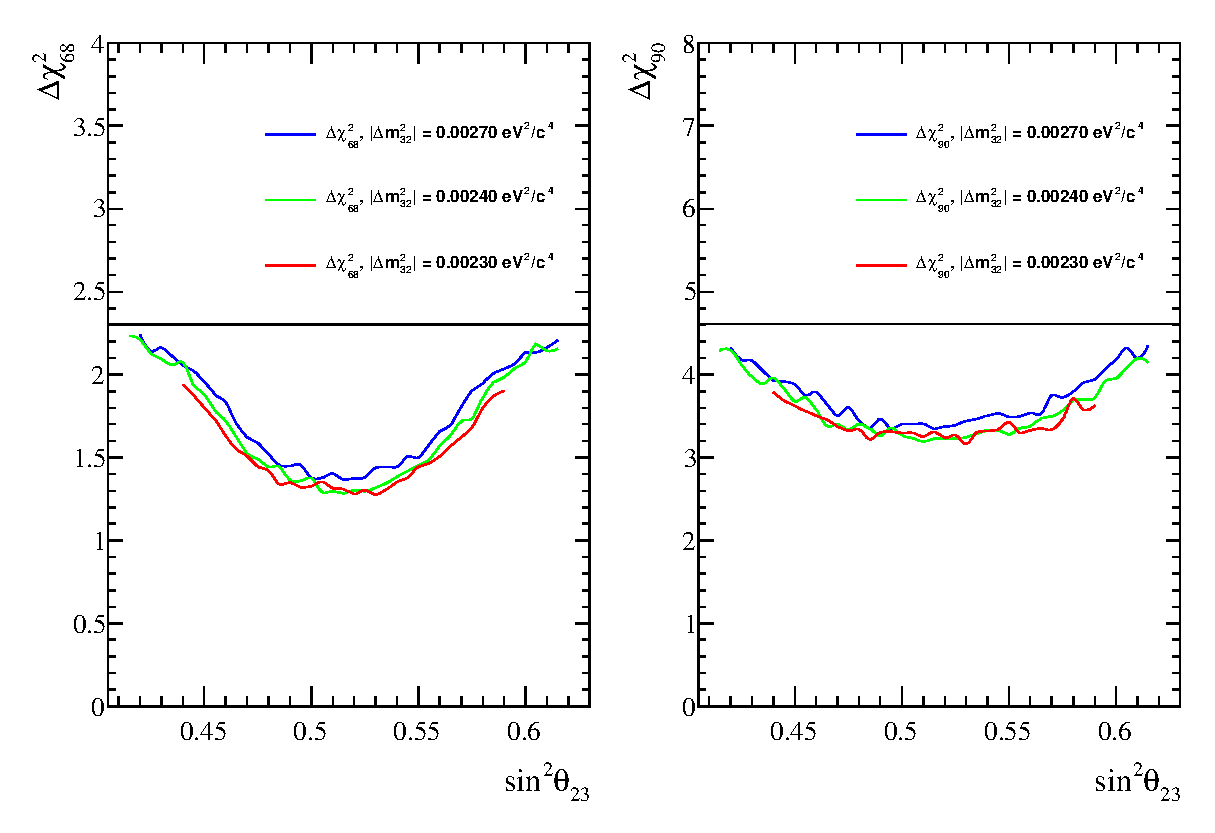
\includegraphics[width=30pc]{./images/fc_surface/FC_slice_mixing_normal}
  \caption {
    1-dimensional slices through the 68\% (left) and 90\% (right) 2-dimensional surfaces of 
    Feldman-Cousins $\Delta\chi^{2}_{critical}$ values
    as a function of $\sin^{2}{\theta_{23}}$ for 3 different values of $|\Delta{m^{2}_{32}}|$
    (2.3$\times$10$^{-3}$ eV$^{2}/c^{4}$,
    2.4$\times$10$^{-3}$ eV$^{2}/c^{4}$ and
    2.7$\times$10$^{-3}$ eV$^{2}/c^{4}$).
    The $\Delta\chi^{2}_{critical}$ values were calculated
    from an ensemble of toy MC experiments, for an exposure of 6.5700$\times$10$^{20}$ POT,
    including both randomized systematic variations and statistical fluctuations.
    For comparison, the canonical value used in the constant-$\Delta\chi^{2}$
    method is also shown as a horizontal line.
    The normal mass hierarchy is assumed.
    $\Delta\chi^2_{critical}$ is only calculated for values of
    $\sin^{2}{\theta_{23}}$ and $|\Delta{m^{2}_{32}}|$
    that affect the 68\% and 90\% confidence contours.
  }
  \label{fig:fc_dchisqcrit_slice_mixing:normal}
\end{figure*}

%.......

\begin{figure*}[htb]
  \center
  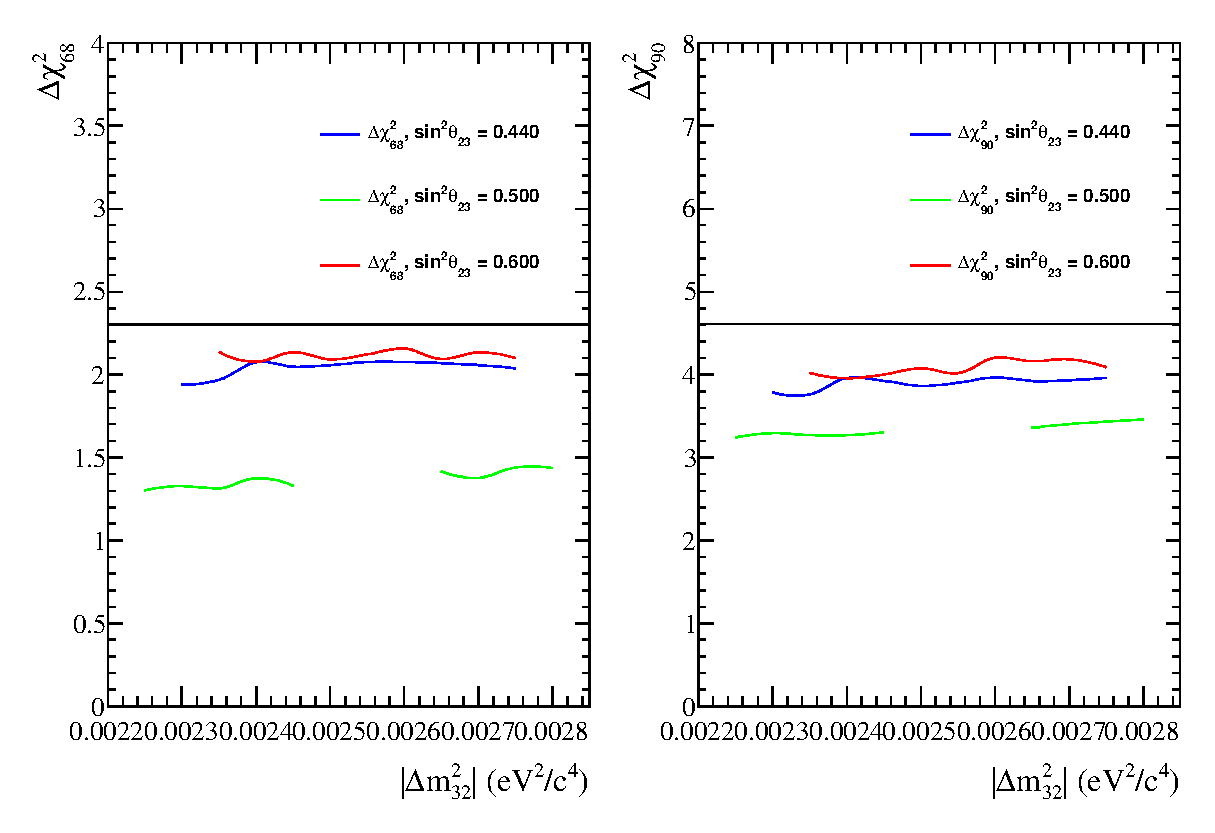
\includegraphics[width=30pc]{./images/fc_surface/FC_slice_dmsq_normal}
  \caption {
    1-dimensional slices through the 68\% (left) and 90\% (right) 2-dimensional surfaces of
    Feldman-Cousins $\Delta\chi^{2}_{critical}$ values
    as a function of $|\Delta{m^{2}_{32}}|$ for 3 different values of $\sin^{2}{\theta_{23}}$
    (0.44, 0.50 and 0.60).
    The $\Delta\chi^{2}_{critical}$ values were calculated
    from an ensemble of toy MC experiments, for an exposure of 6.5700$\times$10$^{20}$ POT,
    including both randomized systematic variations and statistical fluctuations.
    For comparison, the canonical value used in the constant-$\Delta\chi^{2}$
    method is also shown as a horizontal line.
    The normal mass hierarchy is assumed.
    $\Delta\chi^2_{critical}$ is only calculated for values of
    $\sin^{2}{\theta_{23}}$ and $|\Delta{m^{2}_{32}}|$
    that affect the 68\% and 90\% confidence contours.
  }
  \label{fig:fc_dchisqcrit_slice_dmsq:normal}
\end{figure*}

%.......

\begin{figure*}[htb]
  \center
  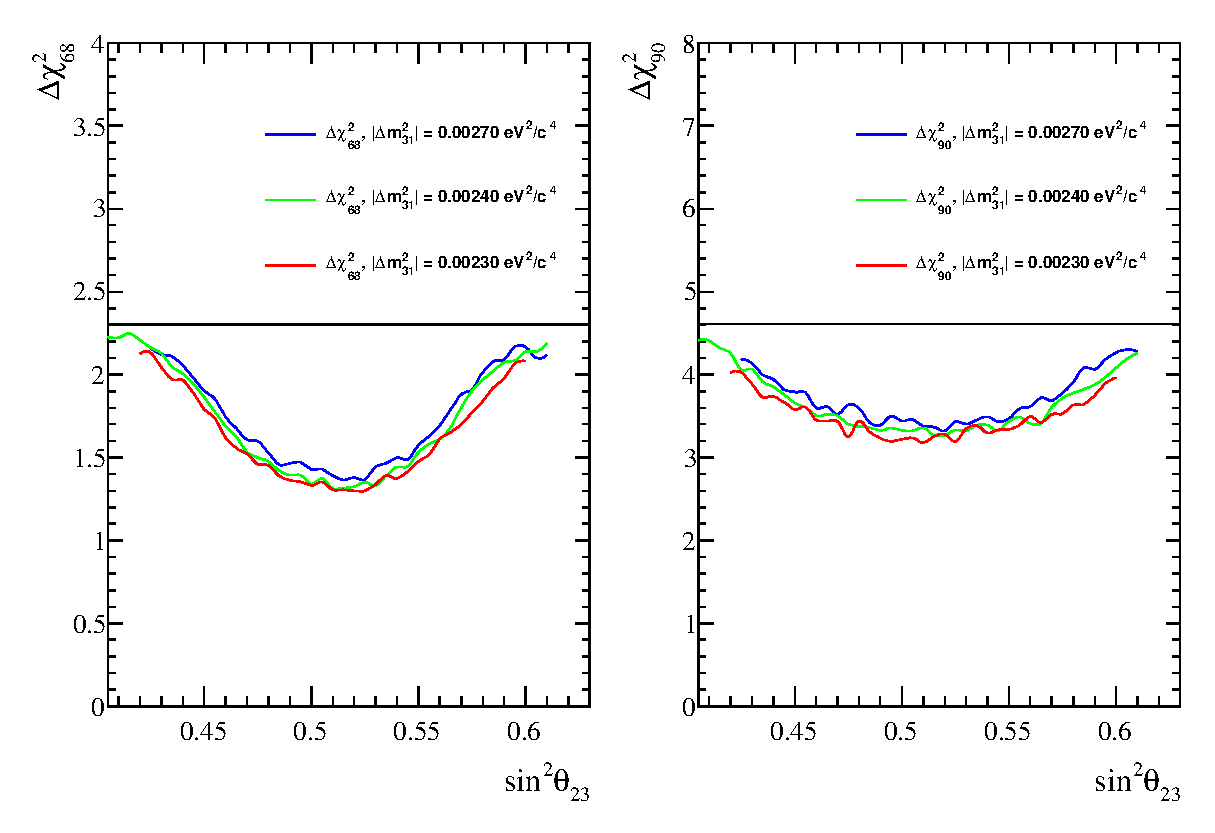
\includegraphics[width=30pc]{./images/fc_surface/FC_slice_mixing_inverted31}
  \caption {
    1-dimensional slices through the 68\% (left) and 90\% (right) 2-dimensional surfaces of
    Feldman-Cousins $\Delta\chi^{2}_{critical}$ values
    as a function of $\sin^{2}{\theta_{23}}$ for 3 different values of $|\Delta{m^{2}_{31}}|$
    (2.3$\times$10$^{-3}$ eV$^{2}/c^{4}$,
    2.4$\times$10$^{-3}$ eV$^{2}/c^{4}$ and
    2.7$\times$10$^{-3}$ eV$^{2}/c^{4}$).
    The $\Delta\chi^{2}_{critical}$ values were calculated
    from an ensemble of toy MC experiments, for an exposure of 6.5700$\times$10$^{20}$ POT,
    including both randomized systematic variations and statistical fluctuations.
    For comparison, the canonical value used in the constant-$\Delta\chi^{2}$
    method is also shown as a horizontal line.
    The inverted mass hierarchy is assumed.
    $\Delta\chi^2_{critical}$ is only calculated for values of
    $\sin^{2}{\theta_{23}}$ and $|\Delta{m^{2}_{31}}|$
    that affect the 68\% and 90\% confidence contours.
  }
  \label{fig:fc_dchisqcrit_slice_mixing:inverted}
\end{figure*}

%.......

\begin{figure*}[htb]
  \center
  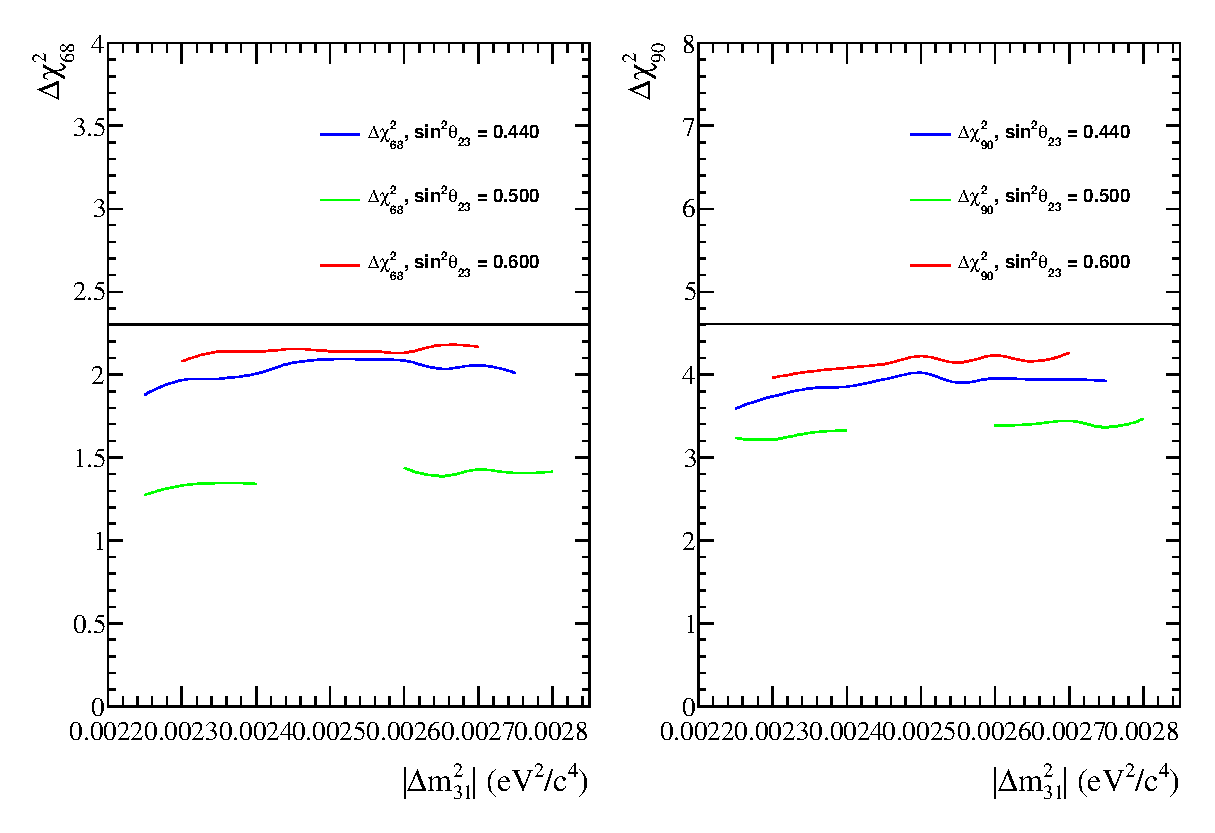
\includegraphics[width=30pc]{./images/fc_surface/FC_slice_dmsq_inverted31}
  \caption {
    1-dimensional slices through the 68\% (left) and 90\% (right) 2-dimensional surfaces of
    Feldman-Cousins $\Delta\chi^{2}_{critical}$ values
    as a function of $|\Delta{m^{2}_{31}}|$ for 3 different values of $\sin^{2}{\theta_{23}}$
    (0.44, 0.50 and 0.60).
    The $\Delta\chi^{2}_{critical}$ values were calculated
    from an ensemble of toy MC experiments, for an exposure of 6.5700$\times$10$^{20}$ POT,
    including both randomized systematic variations and statistical fluctuations.
    For comparison, the canonical value used in the constant-$\Delta\chi^{2}$
    method is also shown as a horizontal line.
    The inverted mass hierarchy is assumed.
    $\Delta\chi^2_{critical}$ is only calculated for values of
    $\sin^{2}{\theta_{23}}$ and $|\Delta{m^{2}_{31}}|$
    that affect the 68\% and 90\% confidence contours.
  }
  \label{fig:fc_dchisqcrit_slice_dmsq:inverted}
\end{figure*}


%...........................................................
%
% FC contours 
% 

\begin{figure*}[htb]
  \center
  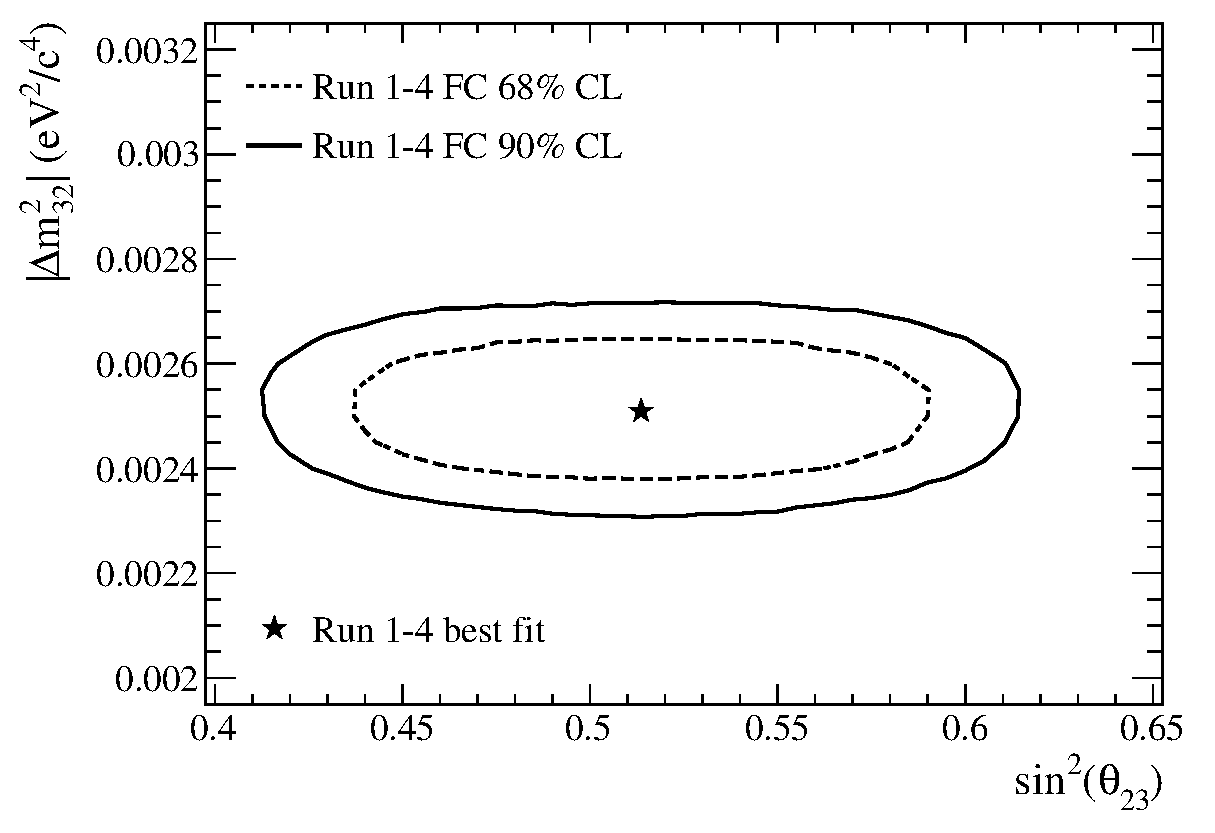
\includegraphics[width=35pc]{./images/data_fit/fc/contour_compare_normal_fconly}
  \caption {
    68\% CL and 90\% CL allowed regions, 
    constructed with the method of Feldman and Cousins,
    from the fit of the Run 1+2+3+4 dataset,
    with the effects of statistical fluctuations and systematic variations being included.
    The best-fit point is also shown.
    The normal mass hierarchy is assumed.
  }
  \label{fig:results_data1234_fc_contour:normal}
\end{figure*}

\begin{figure*}[htb]
  \center
  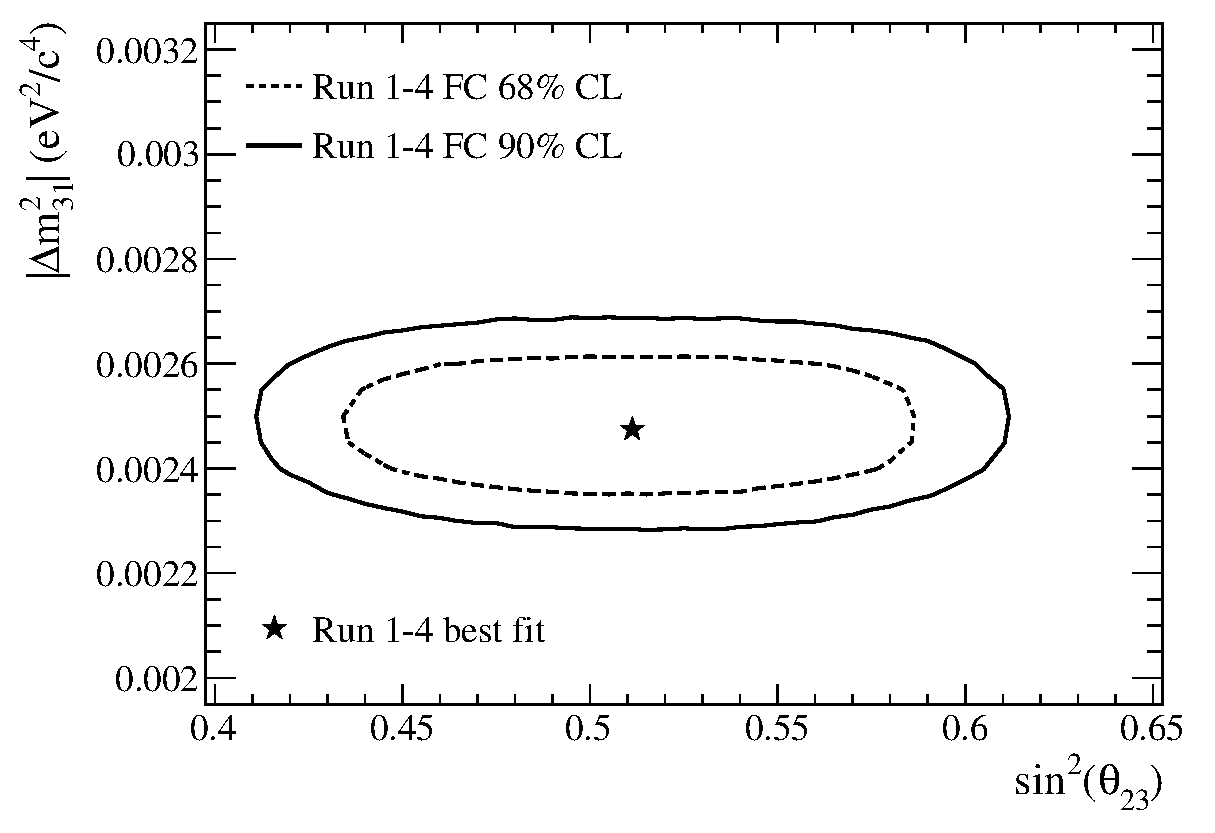
\includegraphics[width=35pc]{./images/data_fit/fc/contour_compare_inverted31_fconly}
  \caption {
    68\% CL and 90\% CL allowed regions, 
    constructed with the method of Feldman and Cousins,
    from the fit to the Run 1+2+3+4 dataset,
    with the effects of statistical fluctuations and systematic variations being included.
    The best-fit point is also shown.
    The inverted mass hierarchy is assumed.
  }
  \label{fig:results_data1234_fc_contour:inverted}
\end{figure*}

\clearpage

%...........................................................                                                                                                                          
%                                                                                                                                                                             
% Profile \Delta\chisquare plots & Table summarizing 1D limits                                                                                                                       
%

\begin{figure*}[htb]
  \begin{minipage}[t]{0.96\linewidth}
    \center
    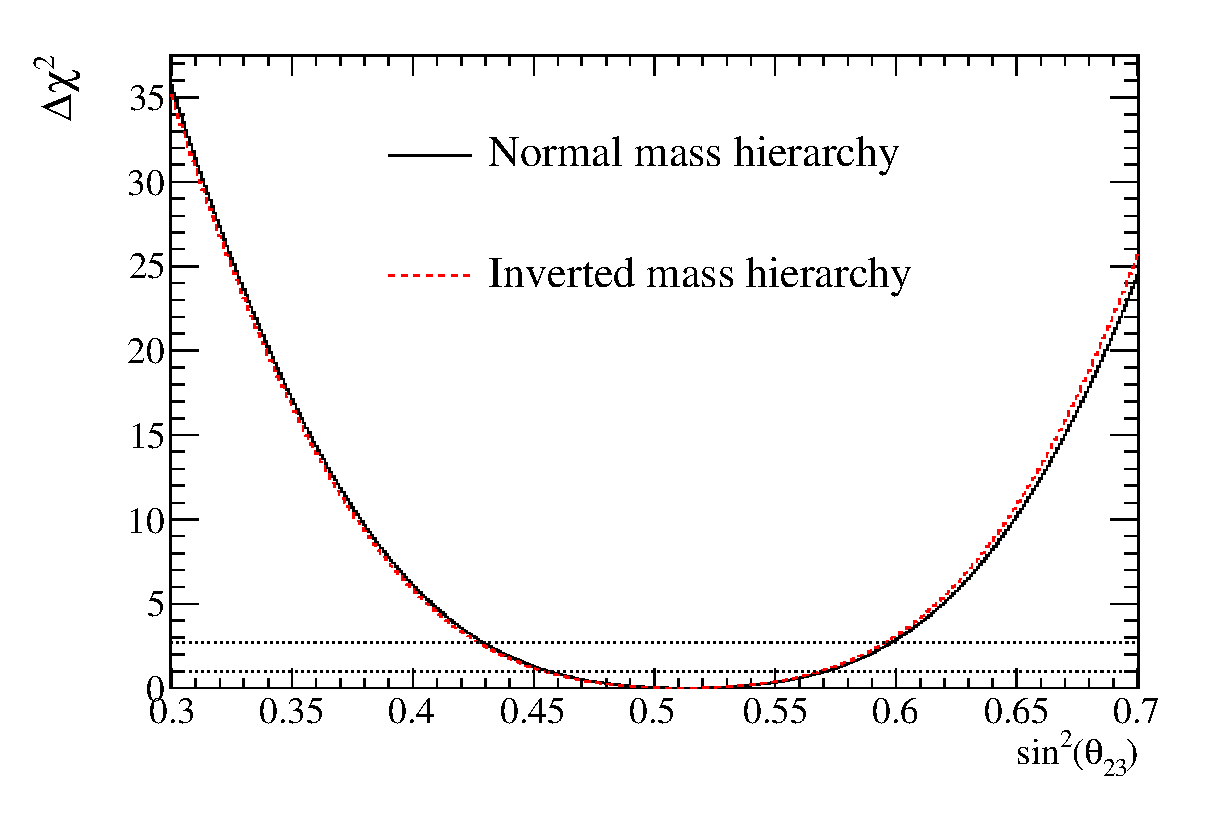
\includegraphics[width=30pc]{./images/data_fit/compare/dchisq_profiles_mix23}
    \caption {
      Profile $\Delta\chi^2$, as a function of $\sin^{2}\theta_{23}$,
      from the 2-parameter fits of the Run 1+2+3+4 dataset.
      The 68\% and 90\% critical constant-$\Delta\chi^{2}$ values
      for one degree of freedom
      are shown as horizontal dotted lines.
    }
    \label{fig:results_marg_dchisq_dmsq_normalinverted}
  \end{minipage}
  \vfill
  \begin{minipage}[t]{0.96\linewidth}
    \center
    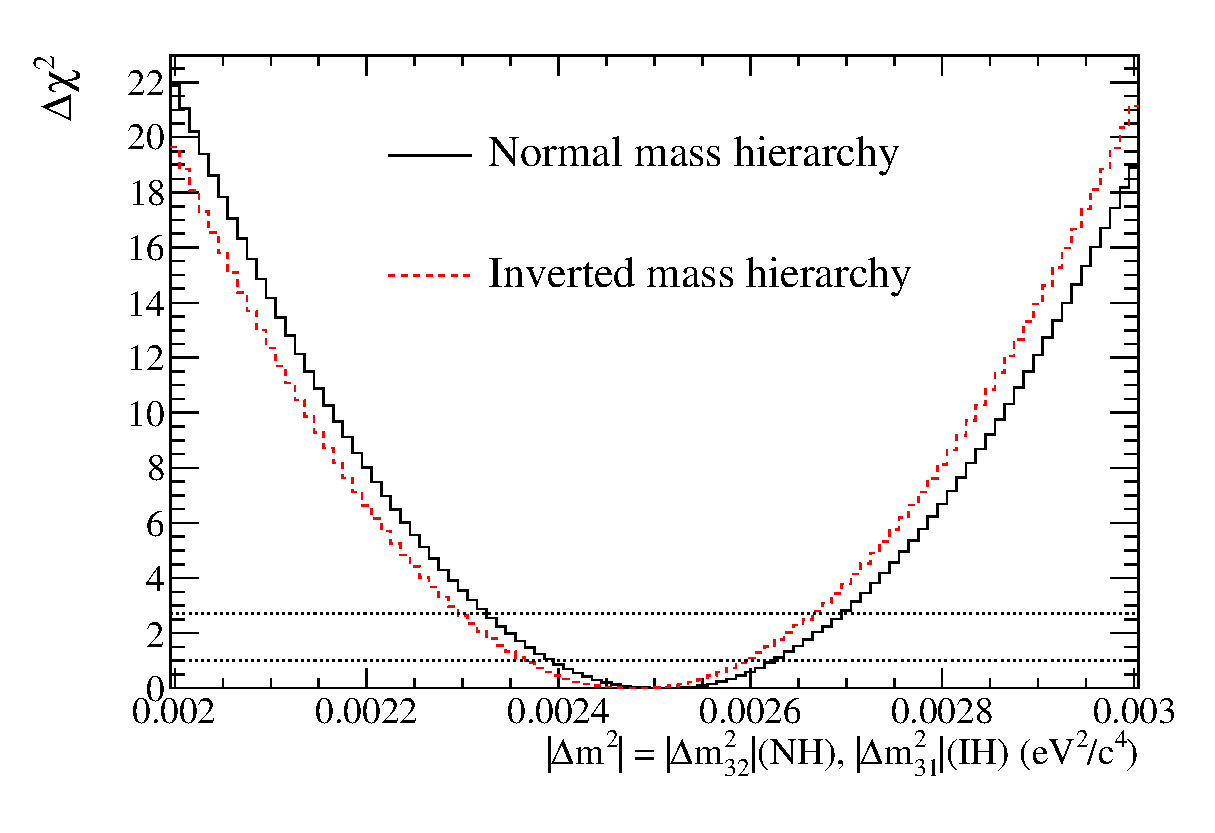
\includegraphics[width=30pc]{./images/data_fit/compare/dchisq_profiles_dm32sq}
    \caption {
      Profile $\Delta\chi^2$, as a function of $|\Delta m^{2}_{32}|$ for the normal mass hierarchy
      and of $|\Delta m^{2}_{31}|$ for the inverted mass hierarchy,
      from the 2-parameter fits of the Run 1+2+3+4 dataset.
      The 68\% and 90\% critical constant-$\Delta\chi^{2}$ values
      for one degree of freedom
      are shown as horizontal dotted lines.
    }
    \label{fig:results_marg_dchisq_sinsq_normalinverted}
  \end{minipage}
\end{figure*}

\begin{figure*}[htb]
\center
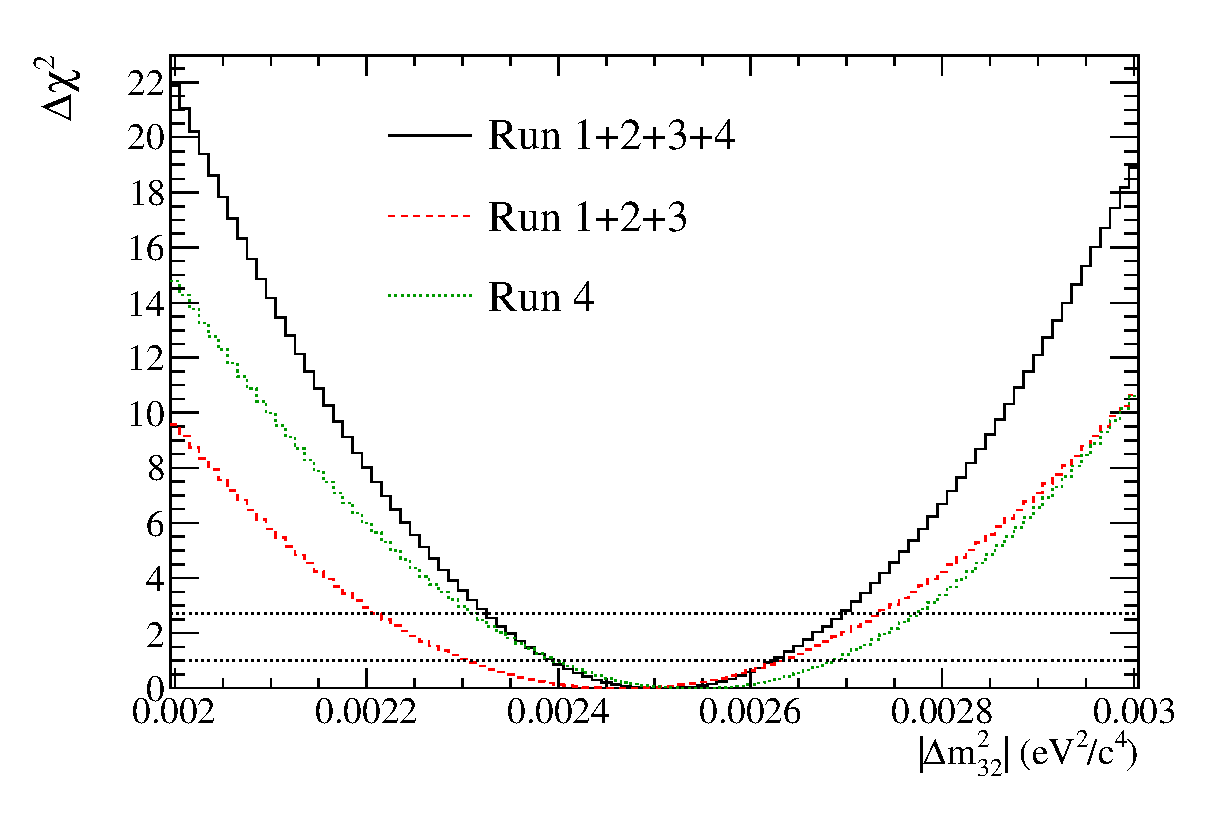
\includegraphics[width=30pc]{./images/data_fit/compare/dchisq_profiles3_dm32sq_sepruns}
\caption {
  Profile $\Delta\chi^2$, as a function of $|\Delta m^{2}_{32}|$,
  from the 2-parameter fits of the Run 1+2+3+4, Run 1+2+3 and Run 4 datasets.
  The normal mass hierarchy is assumed.
}
\label{fig:results_marg_dchisq_dmsq_all3}
\end{figure*}

\begin{figure*}[htb]
\center
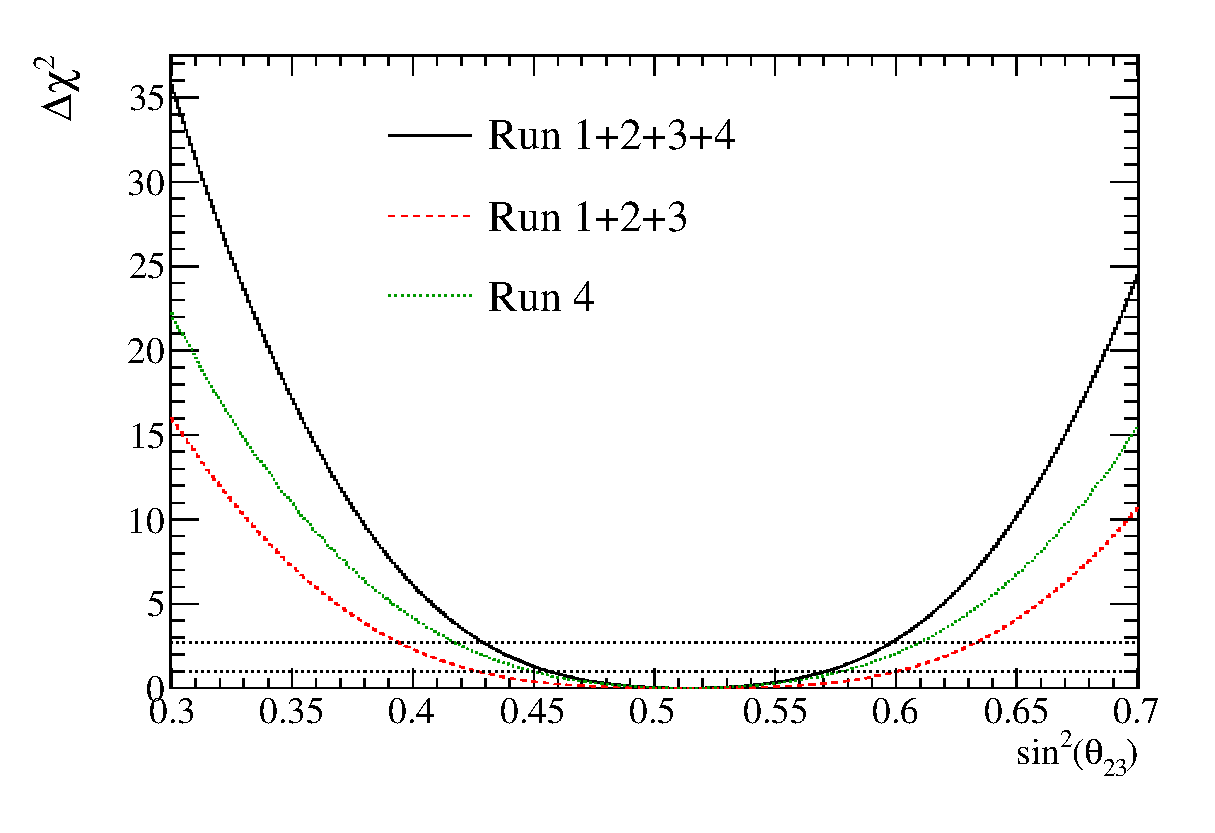
\includegraphics[width=30pc]{./images/data_fit/compare/dchisq_profiles3_mix23_sepruns}
\caption {
  Profile $\Delta\chi^2$, as a function of $\sin^{2}\theta_{23}$,
  from the 2-parameter fits of the Run 1+2+3+4, Run 1+2+3 and Run 4 datasets.
  The normal mass hierarchy is assumed.
}
\label{fig:results_marg_dchisq_sinsq_all3}
\end{figure*}

\begin{figure*}[htb]
  \begin{minipage}[t]{0.96\linewidth}
    \center
    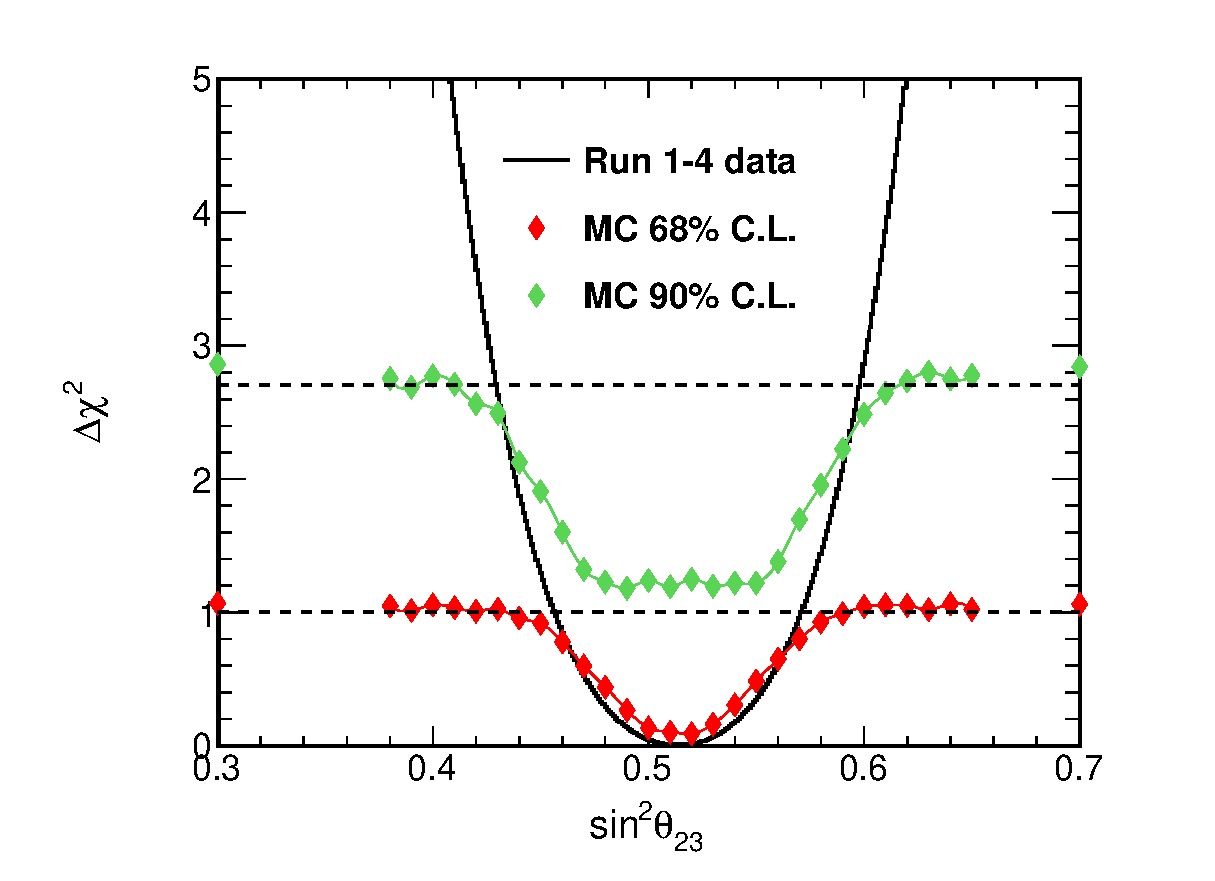
\includegraphics[width=30pc]{./images/data_fit/normal/run1-4_nuis4_sintheta_normal_1DFC_interval}
    \caption {
     Comparison between the 1D $\Delta \chi^{2}$ from the fit of the Run 1+2+3+4 data and the Monte Carlo estimation of the
     1D 68\% and 90\% critical values of $\Delta \chi^{2}$ as a function of $\sin^{2}\theta_{23}$. Each MC
     critical value is obtained from 10000 toy experiments with systematic variations and statistical fluctuations; these
     critical values are fitted with cubic splines. The normal mass hierarchy is assumed.
     The canonical constant-$\Delta \chi^{2}$ 68\% and 90\% critical values for one degree of freedom are shown as dashed lines.
    }
    \label{fig:results_1D_dchisq_sinsq_normal}
  \end{minipage}
  \vfill
  \begin{minipage}[t]{0.96\linewidth}
    \center
    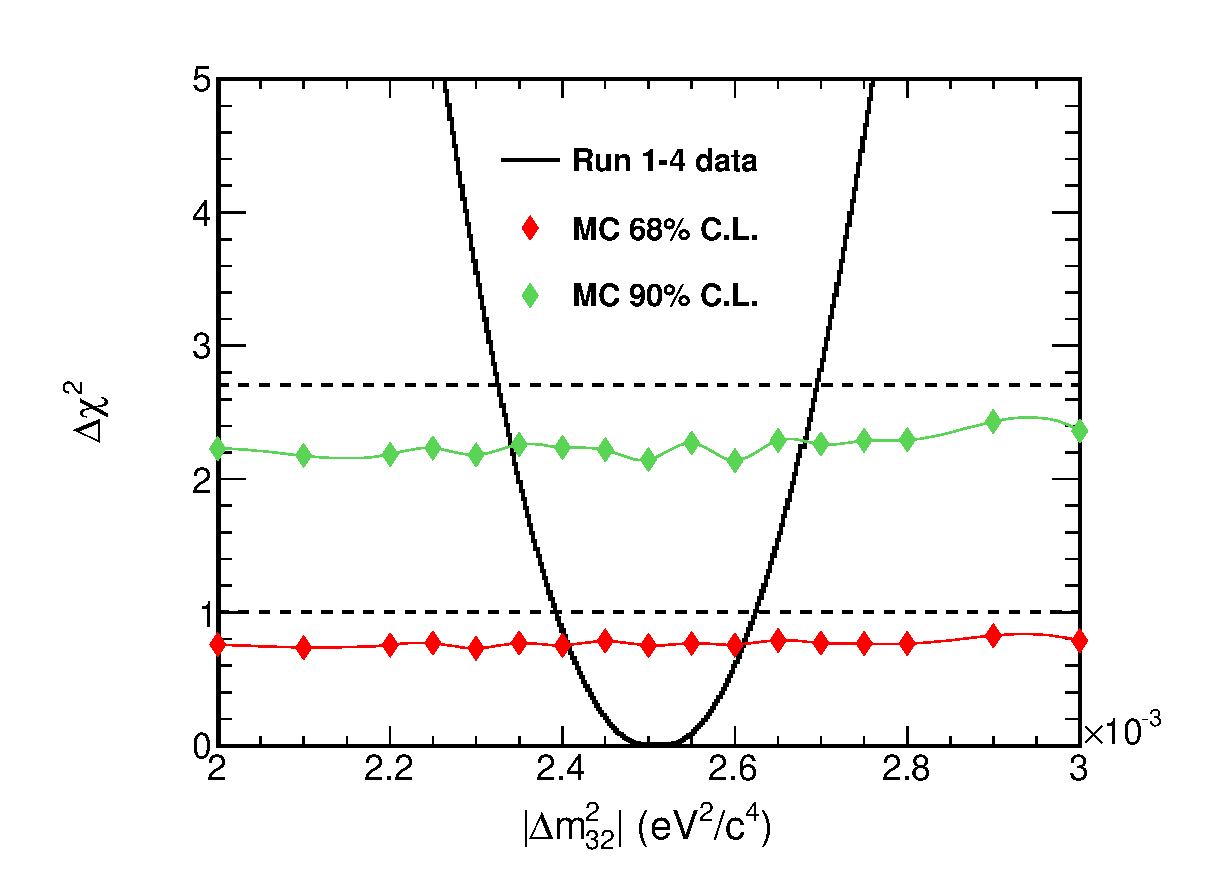
\includegraphics[width=30pc]{./images/data_fit/normal/run1-4_nuis4_dm32sq_normal_1DFC_interval}
    \caption {
     Comparison between the 1D $\Delta \chi^{2}$ from the fit of the Run 1+2+3+4 data and the Monte Carlo estimation of the
     1D 68\% and 90\% critical values of $\Delta \chi^{2}$ as a function of $|\Delta m^{2}_{32}|$. Each MC
     critical value is obtained from 10000 toy experiments with systematic variations and statistical fluctuations; these
     critical values are fitted with cubic splines. The normal mass hierarchy is assumed.
     The canonical constant-$\Delta \chi^{2}$ 68\% and 90\% critical values for one degree of freedom are shown as dashed lines.
    }
    \label{fig:results_1D_dchisq_dm32sq_normal}
  \end{minipage}
\end{figure*}

\begin{figure*}[htb]
  \begin{minipage}[t]{0.96\linewidth}
    \center
    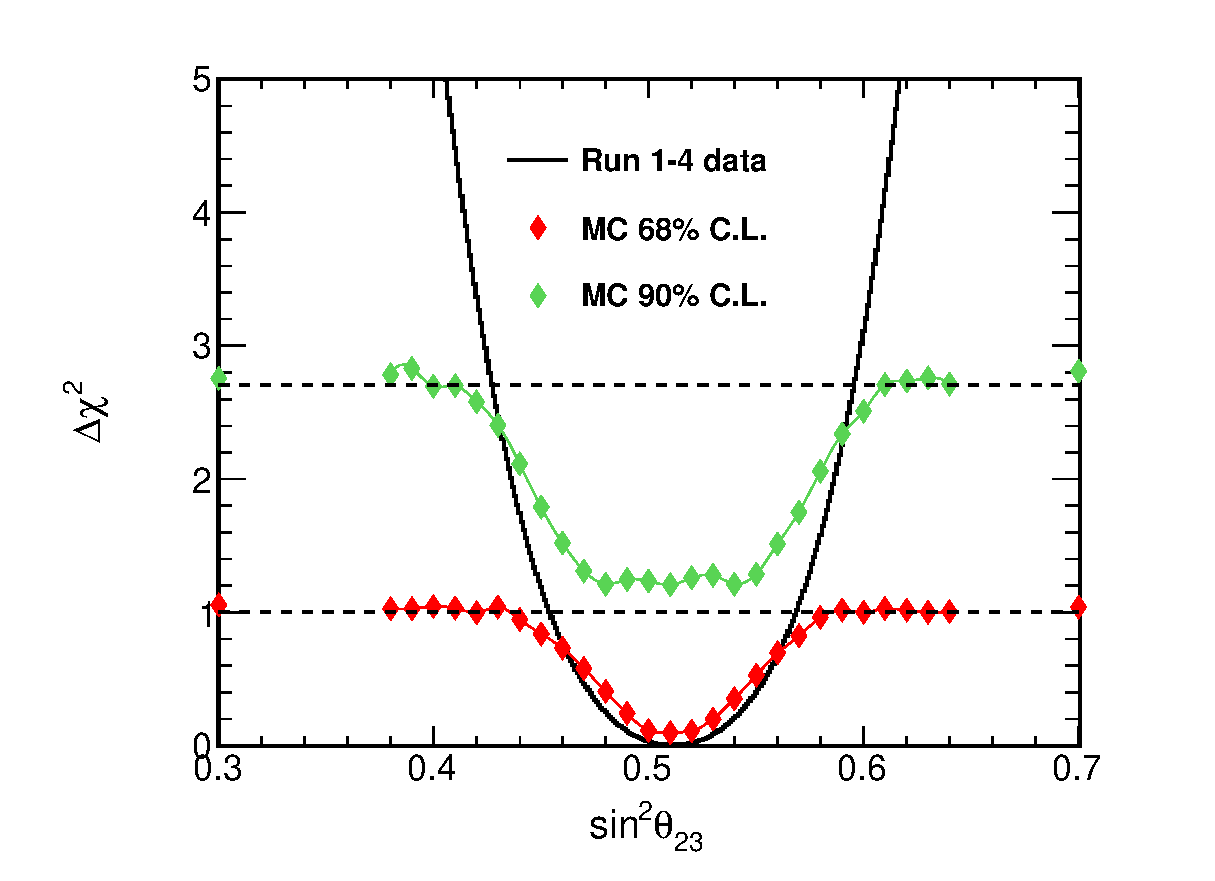
\includegraphics[width=30pc]{./images/data_fit/inverted31/run1-4_nuis4_mixing23_inverted_1DFC_interval}
    \caption {
     Comparison between the 1D $\Delta \chi^{2}$ from the fit of the Run 1+2+3+4 data and the Monte Carlo estimation of the
     1D 68\% and 90\% critical values of $\Delta \chi^{2}$ as a function of $\sin^{2}\theta_{23}$. Each MC
     critical value is obtained from 10000 toy experiments with systematic variations and statistical fluctuations; these
     critical values are fitted with cubic splines. The inverted mass hierarchy is assumed.
     The canonical constant-$\Delta \chi^{2}$ 68\% and 90\% critical values for one degree of freedom are shown as dashed lines.
    }
    \label{fig:results_1D_dchisq_sinsq_inverted}
  \end{minipage}
  \vfill
  \begin{minipage}[t]{0.96\linewidth}
    \center
    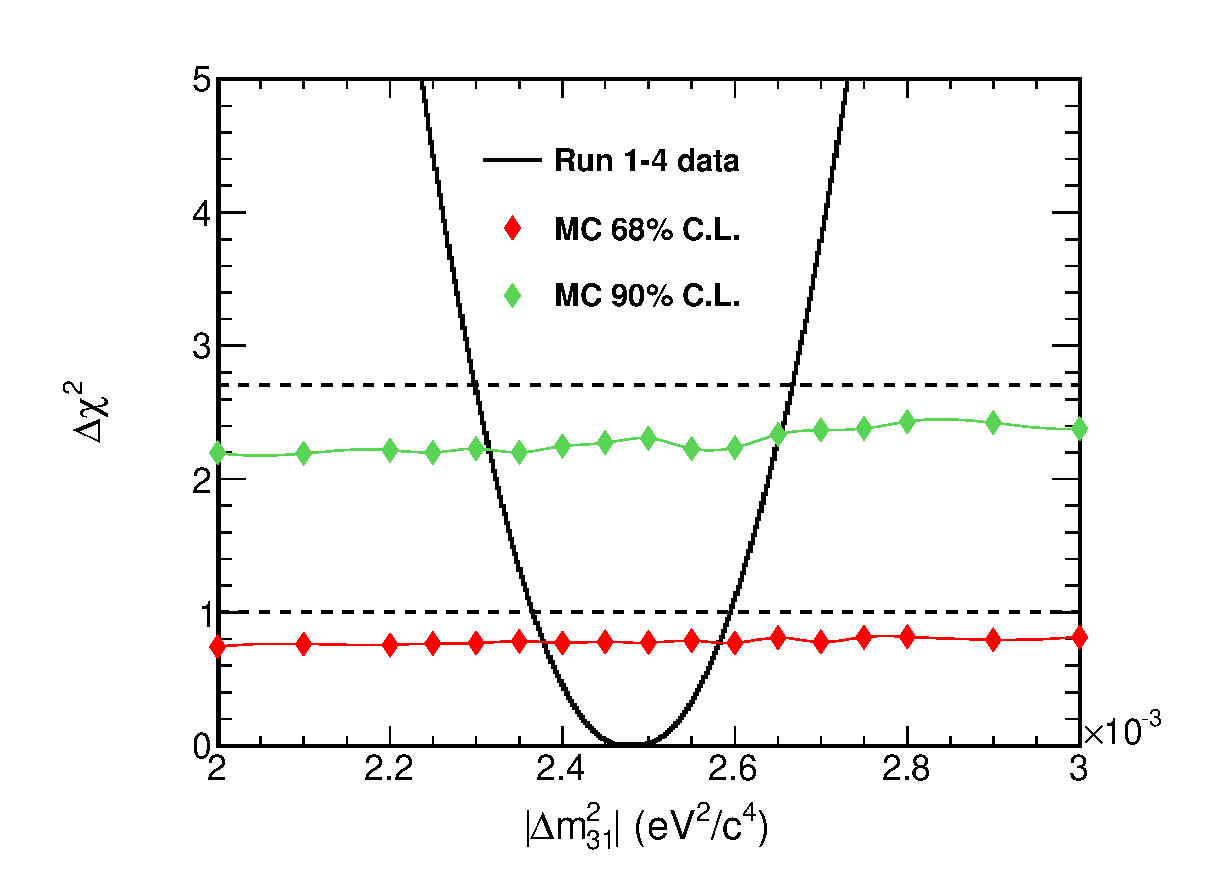
\includegraphics[width=30pc]{./images/data_fit/inverted31/run1-4_nuis4_dm31sq_inverted_1DFC_interval}
    \caption {
     Comparison between the 1D $\Delta \chi^{2}$ from the fit of the Run 1+2+3+4 data and the Monte Carlo estimation of the
     1D 68\% and 90\% critical values of $\Delta \chi^{2}$ as a function of $|\Delta m^{2}_{31}|$. Each MC
     critical value is obtained from 10000 toy experiments with systematic variations and statistical fluctuations; these
     critical values are fitted with cubic splines. The inverted mass hierarchy is assumed.
     The canonical constant-$\Delta \chi^{2}$ 68\% and 90\% critical values for one degree of freedom are shown as dashed lines.
    }
    \label{fig:results_1D_dchisq_dm32sq_inverted}
  \end{minipage}
\end{figure*}

\begin{table}[htb]
  \centering
  \begin{tabular}{| c | c | c | c | D{.}{.}{-1} D{.}{.}{-1} | D{.}{.}{-1}  D{.}{.}{-1} |}
    \hline
    Method  & Dataset & Mass  & Confidence & \multicolumn{2}{c|}{$\sin^{2}\theta_{23}$}
    &  \multicolumn{2}{c|}{$|\Delta m^{2}_{32}|$ or $|\Delta m^{2}_{31}|$}  \\
    & & hierarchy & level  & \multicolumn{2}{c|}{} &  \multicolumn{2}{c|}{(10$^{-3}$ eV$^2$/c$^4$)} \\
    \hline
    \hline
    \multirow{4}{*}{Constant $\Delta\chi^2$} & \multirow{4}{*}{Run 1+2+3+4} & \multirow{2}{*}{Normal} & 68\% & \multicolumn{2}{c|}{\resultNormalMixingErrorsShort} & \multicolumn{2}{c|}{\resultNormalDmsqErrorsShort} \\
    \cline{4-8}
                                             & &             & 90\% & \multicolumn{2}{c|}{\resultNormalMixingTwoSigmaLo \: $<$ $\sin^{2}\theta_{23}$ $<$ \resultNormalMixingTwoSigmaHi}
                                             & \multicolumn{2}{c|}{\resultNormalDmsqTwoSigmaLo \: $<$ $|\Delta m^{2}_{32}|$ $<$ \resultNormalDmsqTwoSigmaHi} \\
    \cline{3-8}
                                             & & \multirow{2}{*}{Inverted} & 68\% & \multicolumn{2}{c|}{\resultInvertedMixingErrorsShort} & \multicolumn{2}{c|}{\resultInvertedDmsqErrorsShort} \\
    \cline{4-8}
                                             & &             & 90\% & \multicolumn{2}{c|}{\resultInvertedMixingTwoSigmaLo \: $<$ $\sin^{2}\theta_{23}$ $<$ \resultInvertedMixingTwoSigmaHi}
                                             & \multicolumn{2}{c|}{\resultInvertedDmsqTwoSigmaLo \: $<$ $|\Delta m^{2}_{31}|$ $<$ \resultInvertedDmsqTwoSigmaHi} \\
    \hline
                                             & \multirow{4}{*}{Run 1+2+3+4} & \multirow{2}{*}{Normal} & 68\% & \multicolumn{2}{c|}{\resultNormalMixingFCErrorsShort} & \multicolumn{2}{c|}{\resultNormalDmsqFCErrorsShort} \\
    \cline{4-8}
    Feldman \&                               & &             & 90\% & \multicolumn{2}{c|}{\resultNormalMixingTwoSigmaFCLo \: $<$ $\sin^{2}\theta_{23}$ $<$ \resultNormalMixingTwoSigmaFCHi}
                                             & \multicolumn{2}{c|}{\resultNormalDmsqTwoSigmaFCLo \: $<$ $|\Delta m^{2}_{32}|$ $<$ \resultNormalDmsqTwoSigmaFCHi} \\
    \cline{3-8}
    Cousins
    & & \multirow{2}{*}{Inverted} & 68\% & \multicolumn{2}{c|}{\resultInvertedMixingFCErrorsShort} & \multicolumn{2}{c|}{\resultInvertedDmsqFCErrorsShort} \\
    \cline{4-8}
                                             & &             & 90\% & \multicolumn{2}{c|}{\resultInvertedMixingTwoSigmaFCLo \: $<$ $\sin^{2}\theta_{23}$ $<$ \resultInvertedMixingTwoSigmaFCHi}
                                             & \multicolumn{2}{c|}{\resultInvertedDmsqTwoSigmaFCLo \: $<$ $|\Delta m^{2}_{31}|$ $<$ \resultInvertedDmsqTwoSigmaFCHi} \\
    \hline
    \hline
    \multirow{2}{*}{Constant $\Delta\chi^2$} & \multirow{2}{*}{Run 1+2+3} & \multirow{2}{*}{Normal} & 68\% &
                          \multicolumn{2}{c|}{\resultNormalRunITIIIMixingErrorsShort} & \multicolumn{2}{c|}{\resultNormalRunITIIIDmsqErrorsShort} \\
    \cline{4-8}
                                             & &             & 90\% & \multicolumn{2}{c|}{\resultNormalRunITIIIMixingTwoSigmaLo \: $<$ $\sin^{2}\theta_{23}$ $<$ \resultNormalRunITIIIMixingTwoSigmaHi}
                                             & \multicolumn{2}{c|}{\resultNormalRunITIIIDmsqTwoSigmaLo \: $<$ $|\Delta m^{2}_{32}|$ $<$ \resultNormalRunITIIIDmsqTwoSigmaHi} \\
    \hline
    \multirow{2}{*}{Constant $\Delta\chi^2$} & \multirow{2}{*}{Run 4} & \multirow{2}{*}{Normal} & 68\% &
                          \multicolumn{2}{c|}{\resultNormalRunIVMixingErrorsShort} & \multicolumn{2}{c|}{\resultNormalRunIVDmsqErrorsShort} \\
    \cline{4-8}
                                             & &             & 90\% & \multicolumn{2}{c|}{\resultNormalRunIVMixingTwoSigmaLo \: $<$ $\sin^{2}\theta_{23}$ $<$ \resultNormalRunIVMixingTwoSigmaHi}
                                             & \multicolumn{2}{c|}{\resultNormalRunIVDmsqTwoSigmaLo \: $<$ $|\Delta m^{2}_{32}|$ $<$ \resultNormalRunIVDmsqTwoSigmaHi} \\
    \hline
  \end{tabular}
  \caption{
    Summary of one-dimensional limits on $\sin^{2}\theta_{23}$ and $|\Delta m^{2}_{32}|$ or
    $|\Delta m^{2}_{31}|$ from the fits of the Run 1+2+3, Run 4, and Run 1+2+3+4 datasets.
    The limits are shown for both the constant-$\Delta\chi^2$ method and the new procedure
    described in Sec.\ \ref{sec:contour_construction}.
   }
  \label{tab:data_fits:1dlimits}
\end{table}

\clearpage

%--------------------------------------------------------------------------------------
% Contour comparisons
%--------------------------------------------------------------------------------------

\subsection {Comparisons of confidence regions}
\label{sec:results_contour_comparisons}

A comparison is shown in Fig.\ \ref{fig:results_compare_normal_inverted:constdchisq}
between the Run 1+2+3+4 2-dimensional confidence regions for the normal and inverted mass hierarchies  
obtained using the constant-$\Delta\chi^2$ method (the vertical axis is $|\Delta m_{32}^{2}|$ for the normal mass hierarchy and 
$|\Delta m_{31}^{2}|$ for the inverted mass hierarchy). The equivalent comparison between confidence regions for the two mass 
hierarchies obtained using the Feldman-Cousins method is shown in Fig.\ \ref{fig:results_compare_normal_inverted:fc}.

The Run 1+2+3+4 2-dimensional confidence regions obtained using the constant-$\Delta\chi^2$ and Feldman-Cousins methods
are compared in Fig.\ \ref{fig:results_compare_FC_constdchisq:normal} for the normal mass hierarchy and 
Fig.\ \ref{fig:results_compare_FC_constdchisq:inverted} for the inverted mass hierarchy.
The Feldman-Cousins confidence regions are narrower along $|\Delta{m^{2}_{32}}|$ or $|\Delta{m^{2}_{31}}|$ at maximal disappearance than
those made with the constant-$\Delta\chi^{2}$ method since the Feldman-Cousins $\Delta\chi^2_{critical}$ values are lower 
than the canonical constant-$\Delta\chi^2$ values as explained in Sec.\ \ref{sec:results_contours}. This narrowing of the 
2-dimensional confidence contour was also seen in our earlier Run 1+2 and Run 1+2+3 analyses 
\cite{OurRun12DisappAnalysis,OurRun123DisappAnalysis3Flavour} in which we fitted 
$\sin^{2}{2\theta_{23}}$ instead of $\sin^{2}{\theta_{23}}$. In this analysis, the Feldman-Cousins contours are also 
very slightly narrower in $\sin^{2}{\theta_{23}}$ for values of $|\Delta{m^{2}_{32}}|$ or $|\Delta{m^{2}_{31}}|$ near the best fit.

In Figs.\ \ref{fig:results_compare_FC_constdchisq_external} and \ref{fig:results_compare_FC_constdchisq_external_inverted},
the T2K Run 1+2+3+4 90\% confidence region is compared with 
those from MINOS (2013) \cite{MINOS2013sinsqtheta}, SuperK atmospherics 
(2013 3-flavour 
zenith-angle analysis) \cite{SKAtm2012},
and T2K Run 1+2+3 \cite{T2KRun123Disapp}, for the normal and inverted hierarchies respectively.
A second comparison with external results is shown in Fig.\ \ref{fig:results_compare_FC_constdchisq_external_sinsqtheta23}: 
this figure compares the T2K Run 1+2+3+4 90\% confidence region with
those from MINOS (2013) \cite{MINOS2013}, SuperK atmospherics 
(2012 2-flavour L/E and 3-flavour 
zenith-angle analyses) \cite{SKAtm2012},
and T2K Run 1+2+3 \cite{T2KRun123Disapp},
for the normal mass hierarchy only.
In this plot, the T2K Run 1+2+3+4 fit result has been converted from $\sin^2\theta_{23}$ to
$\sin^2(2\theta_{23})$ by profiling the octant.
This is the same method as that used by SuperK in their zenith angle contour, and,
if this method had been applied to the T2K Run 1+2+3 result, it should have
closely matched the T2K Run 1+2+3 $\theta_{23} \geq \pi/4$ contour.
These plots show that T2K now has the world's best limit in $\theta_{23}$.

In Fig.\ \ref{fig:results_compare_constdchisq_sensitivity_normal}
a comparison is shown
between the Run 1+2+3+4 allowed region obtained 
with constant-$\Delta\chi^{2}$ method and the T2K 6.5700$\times$10$^{20}$ POT sensitivity
contour produced at our best-fit point for the Run 1+2+3+4 dataset.
The 'stat-only' sensitivity contours were computed by averaging the contours of 300 toy MC
experiments generated with statistical fluctuations and all systematic parameters fixed at
their nominal values.
The 'stat+syst' sensitivity contours were computed by averaging the contours of 300 toy MC
experiments generated with statistical fluctuations and all systematic parameters randomized.
As can be seen in the the plot, the T2K data results in a smaller contour than the sensitivity,
particularly for the $\sin^2\theta_{23}$ limit.
p-values can be calculated by comparing the data constant-$\Delta\chi^2$ limits
with the limits of the 'stat+syst' sensitivity fits, and represent the fraction of toy experiments that  provide a \emph{tighter} limit than the data.
For $\sin^2\theta_{23}$ the p-values are 0.21(0.19) for 68\% C.L. and 0.19(0.21) for 90\% C.L. for the lower(upper) limits respectively.
For $|\Delta m^2_{32}|$ the p-values are 0.31(0.20) for 68\% C.L. and 0.42(0.27) for 90\% C.L. for the lower(upper) limit respectively.
This shows that the data are not an extreme fluctuation.
% {\color{red} why not FC? - area is bigger than the surface we have}.

Finally, a comparison between the confidence regions obtained by three 
separate analyses of the Run 1+2+3+4, Run 1+2+3 and Run 4 datasets 
is shown in Fig.\ \ref{fig:results_compare_runs}.
The contours from the different running periods are consistent.

% ......................
% 
% const Delta & FC \chisq normal vs inverted
% 
\begin{figure*}[htb]
  \center
  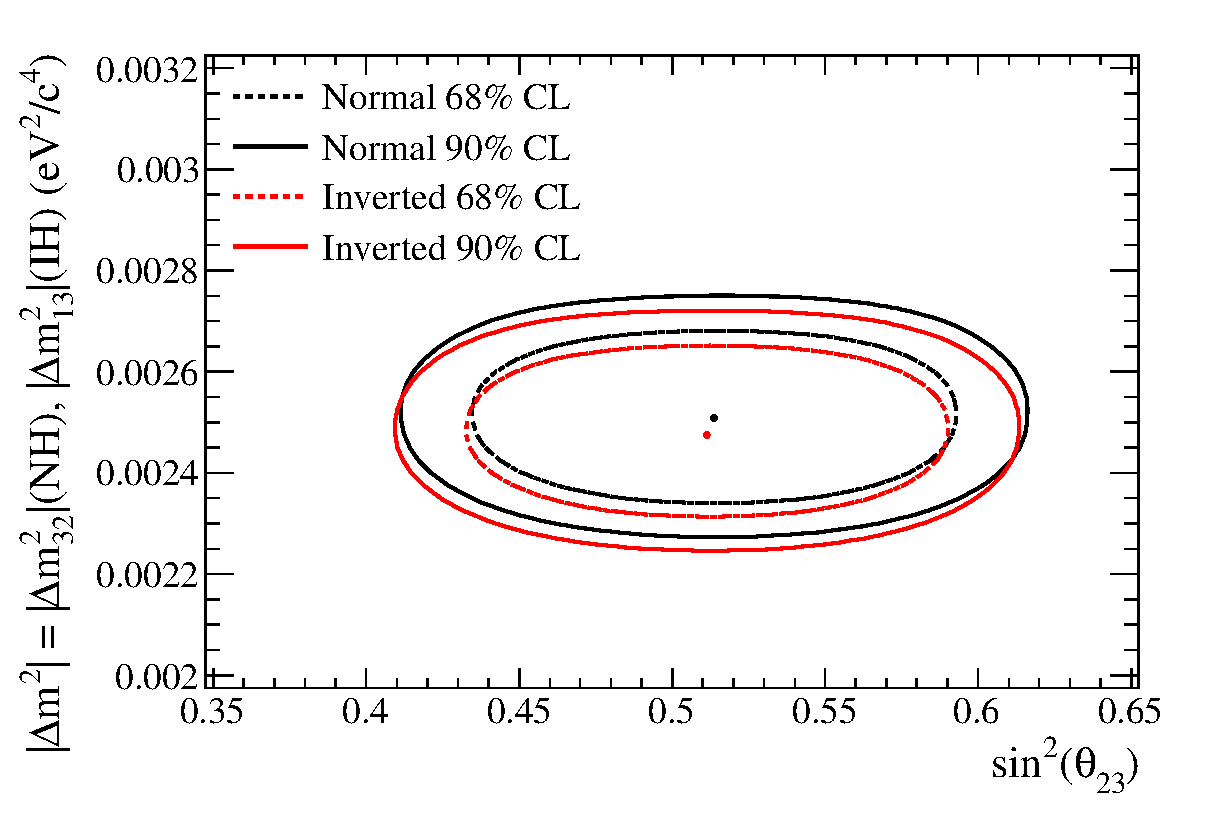
\includegraphics[width=30pc]{./images/data_fit/compare/contours_run1-4_nuis4_hierarchy}
  \caption {
    Comparison between the 68\% CL and 90\% CL allowed regions 
    for the normal and inverted mass hierarchies
    obtained using the constant-$\Delta\chi^2$ method
    from the fit of the Run 1+2+3+4 dataset.
  }
  \label{fig:results_compare_normal_inverted:constdchisq}
\end{figure*}

\begin{figure*}[htb]
  \center
  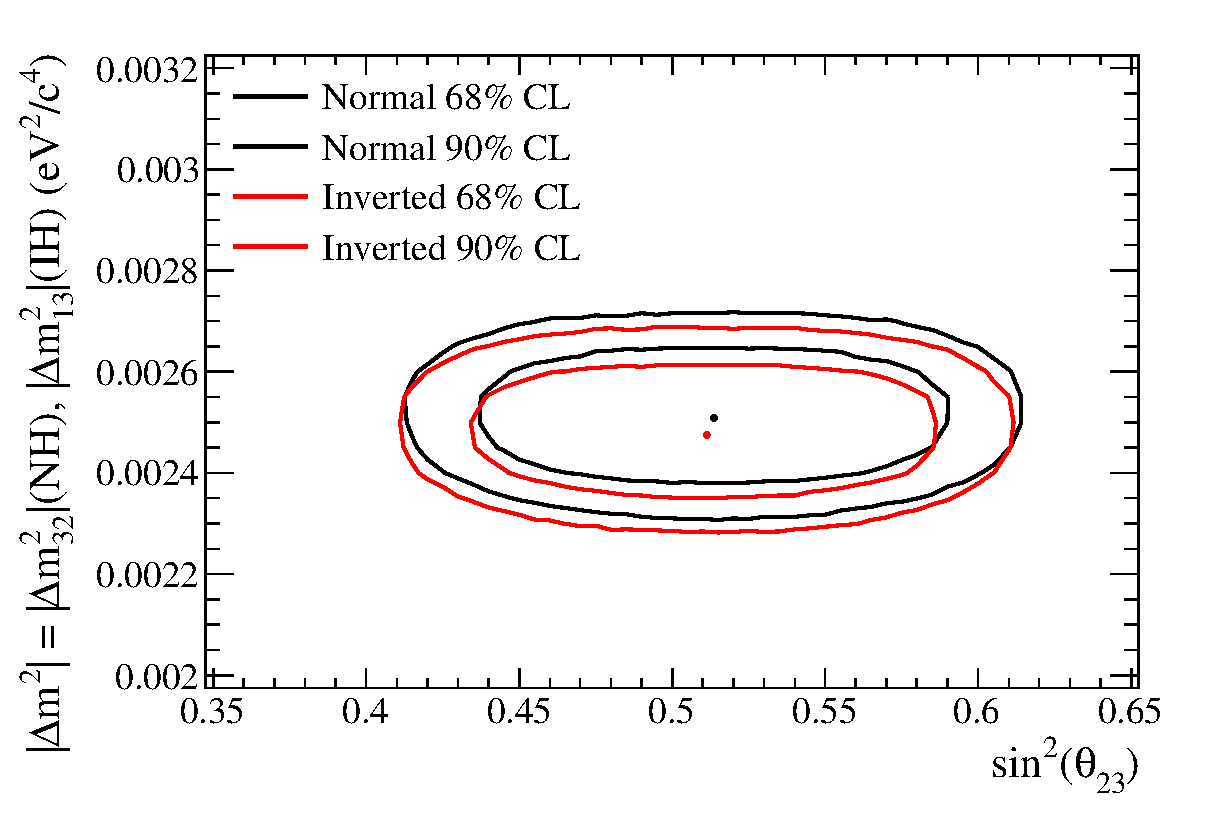
\includegraphics[width=30pc]{./images/data_fit/fc/contour_compare_hierarchies_fc}
  \caption {
    Comparison between the 68\% CL and 90\% CL allowed regions 
    for the normal and inverted mass hierarchies
    obtained using the Feldman-Cousins method
    from the fit of the Run 1+2+3+4 dataset.
  }
  \label{fig:results_compare_normal_inverted:fc}
\end{figure*}

% ......................
% 
% const Delta\chisq vs FC (normal and inverted)
% 
\begin{figure*}[htb]
  \center
  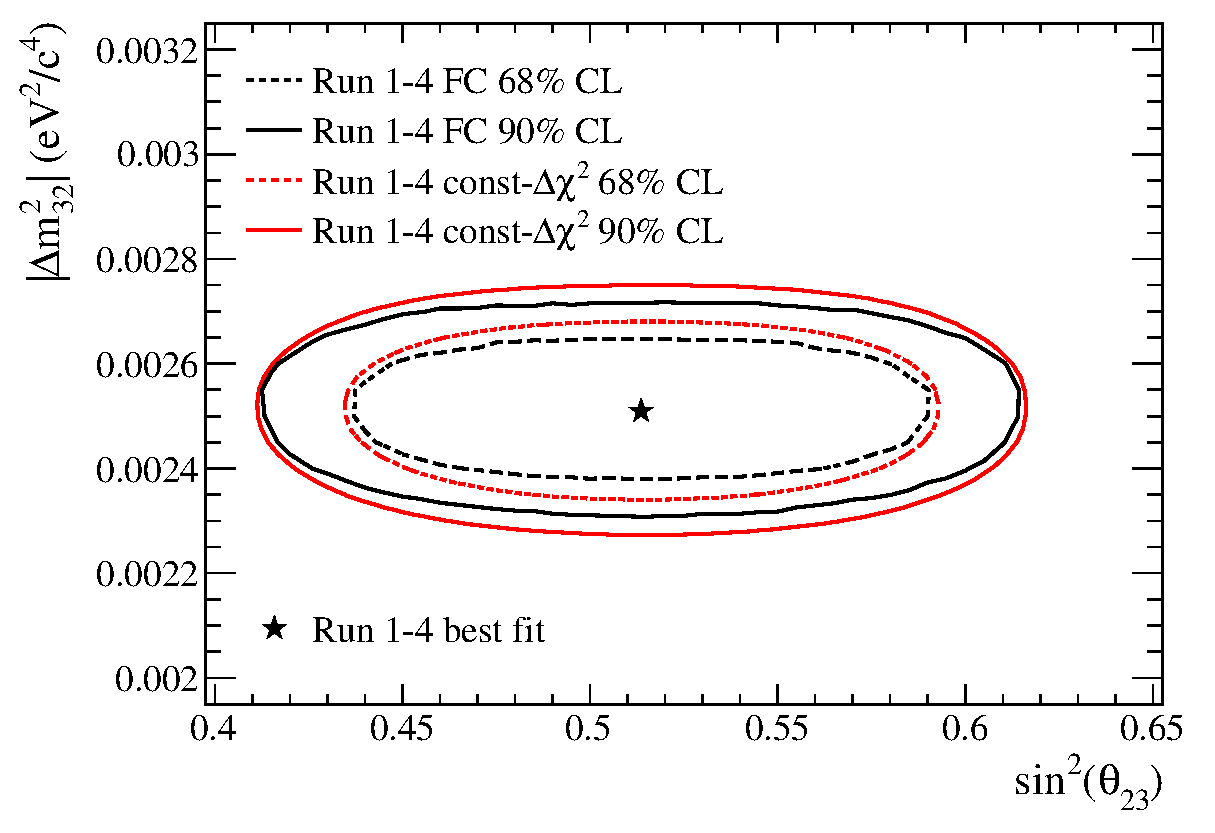
\includegraphics[width=30pc]{./images/data_fit/fc/contour_compare_normal_dcvsfc}
  \caption {
    Comparison between the 68\% CL and 90\% CL allowed regions 
    obtained using the constant-$\Delta\chi^2$ and Feldman-Cousins methods 
    from the fit of the Run 1+2+3+4 dataset.
    The normal mass hierarchy is assumed.
  }
  \label{fig:results_compare_FC_constdchisq:normal}
\end{figure*}

\begin{figure*}[htb]
  \center
  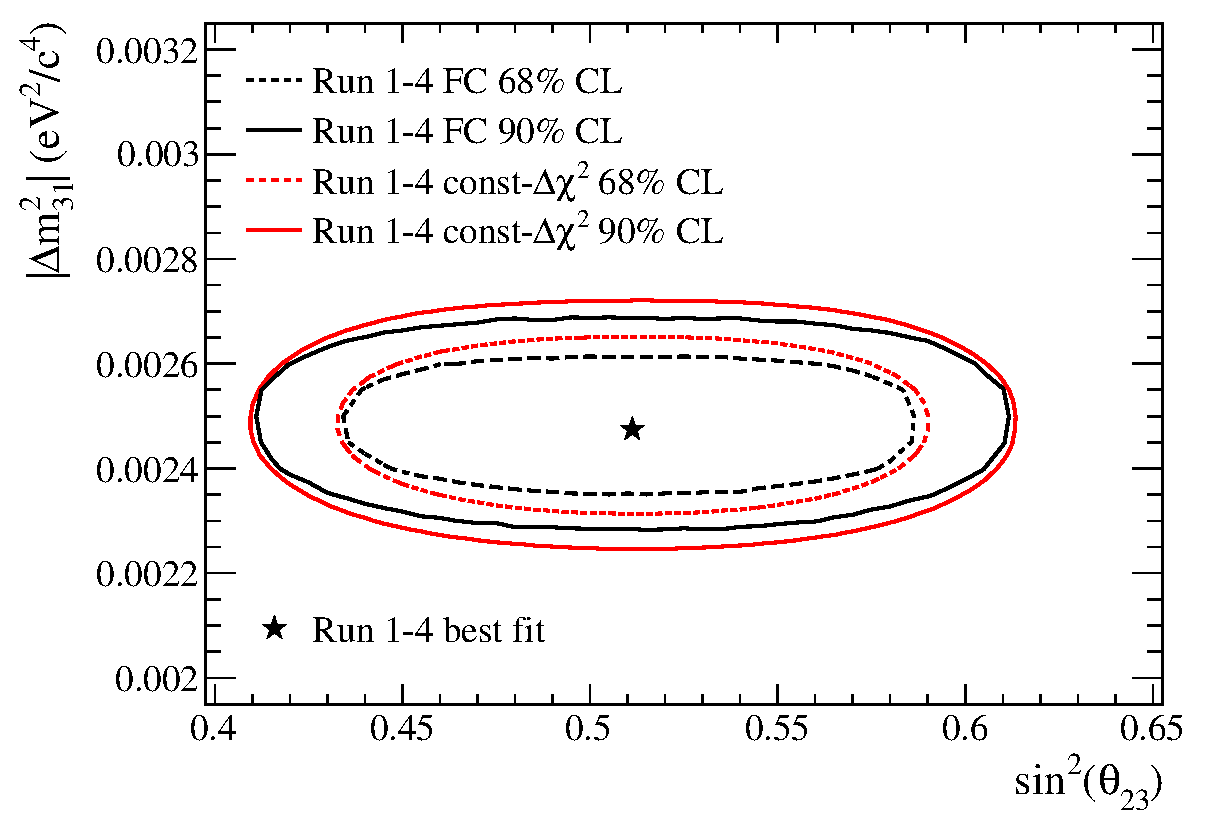
\includegraphics[width=30pc]{./images/data_fit/fc/contour_compare_inverted31_dcvsfc}
  \caption {
    Comparison between the 68\% CL and 90\% CL allowed regions 
    obtained using the constant-$\Delta\chi^2$ and Feldman-Cousins methods 
    from the fit to the Run 1+2+3+4 dataset.
    The inverted mass hierarchy is assumed.
  }
  \label{fig:results_compare_FC_constdchisq:inverted}
\end{figure*}


%......................
%
% VALOR vs the world
% 
\begin{figure*}[htb]
  \center
  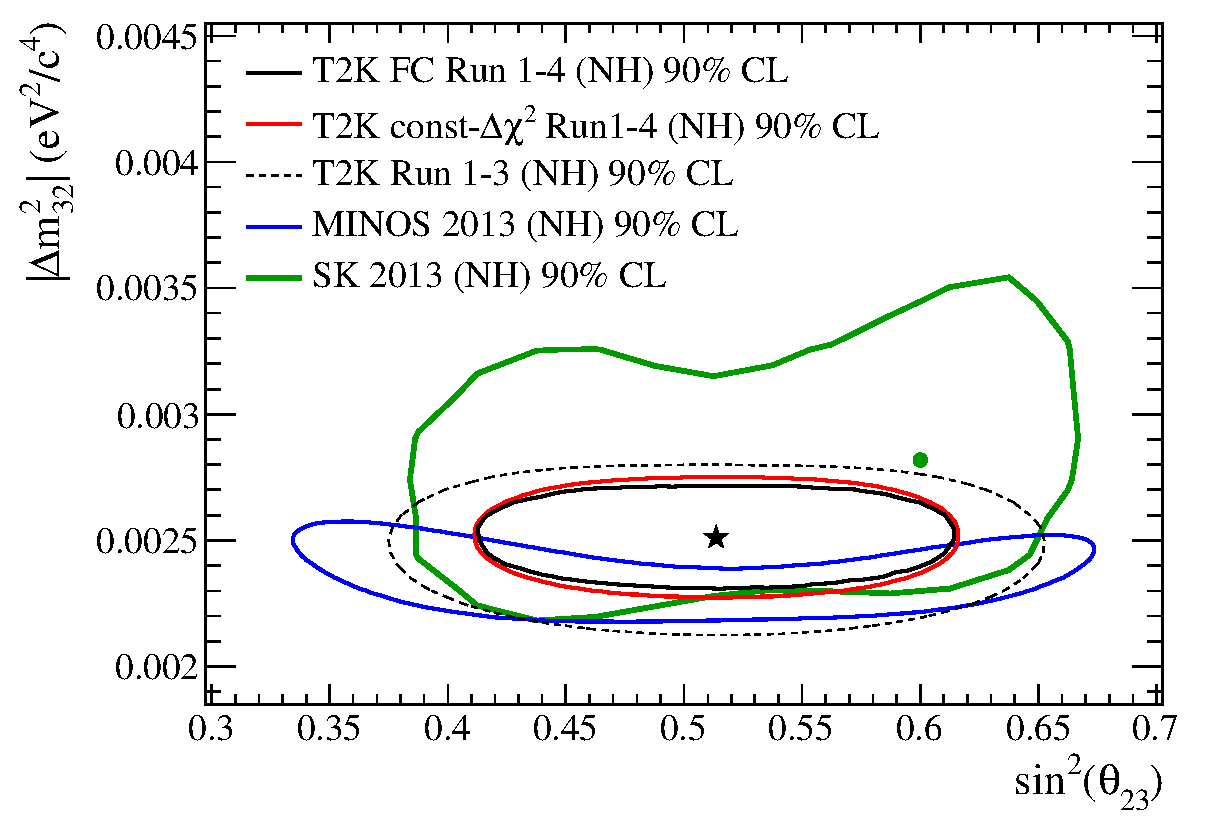
\includegraphics[width=30pc]{./images/data_fit/fc/contour_compare_normal_dcvsfc_ext}
  \caption {
    Comparison between 90\% CL allowed regions 
    from MINOS \cite{MINOS2013sinsqtheta}, SuperK atmospherics \cite{SKAtm2012}, T2K Run 1+2+3 \cite{T2KRun123Disapp},
    and the 90\% CL region obtained from the {\em VALOR} fit of the Run 1+2+3+4 dataset.
    Contours obtained using both the constant-$\Delta\chi^2$ and Feldman-Cousins methods are shown.
    The normal mass hierarchy is assumed for all results.
  }
  \label{fig:results_compare_FC_constdchisq_external}
\end{figure*}

\begin{figure*}[htb]
  \center
  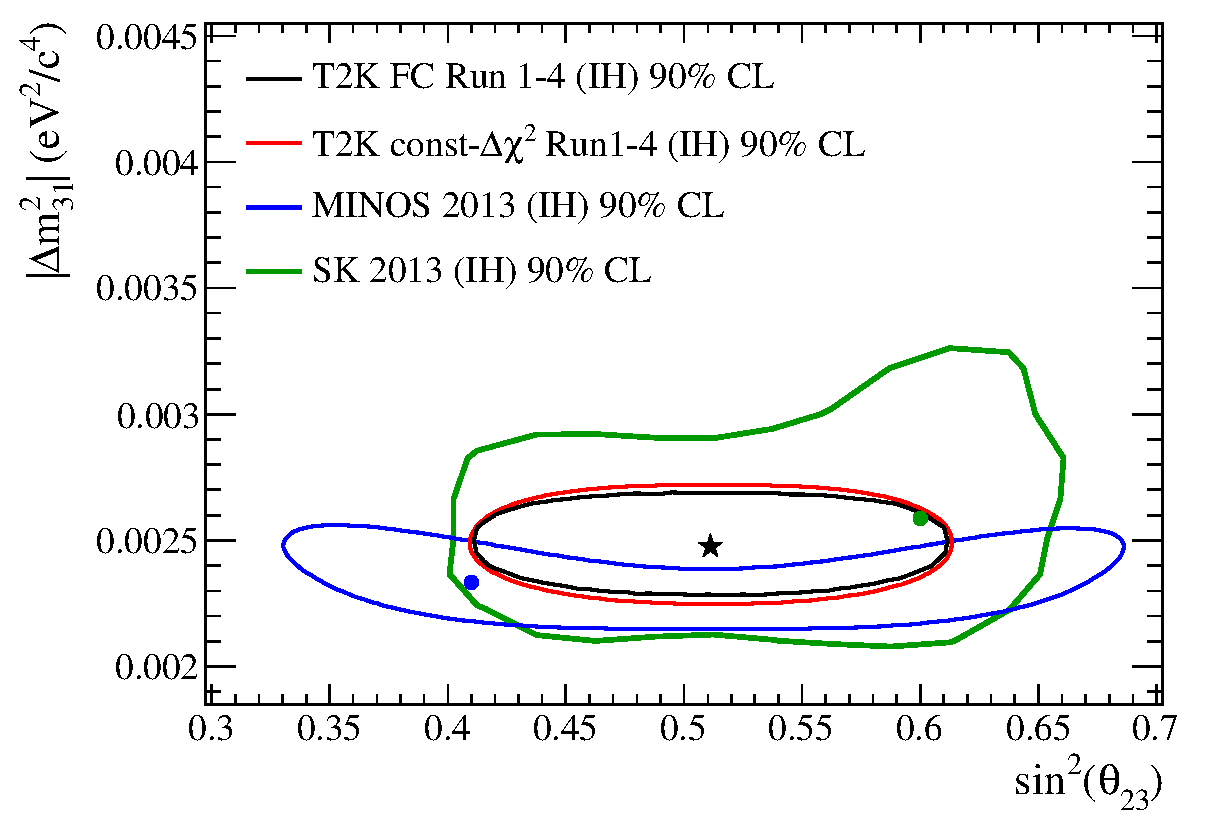
\includegraphics[width=30pc]{./images/data_fit/fc/contour_compare_inverted31_dcvsfc_ext}
  \caption {
    Comparison between 90\% CL allowed regions 
    from MINOS \cite{MINOS2013sinsqtheta}, SuperK atmospherics \cite{SKAtm2012}, T2K Run 1+2+3 \cite{T2KRun123Disapp},
    and the 90\% CL region obtained from the {\em VALOR} fit of the Run 1+2+3+4 dataset.
    Contours obtained using both the constant-$\Delta\chi^2$ and Feldman-Cousins methods are shown.
    The inverted mass hierarchy is assumed for all results.
  }
  \label{fig:results_compare_FC_constdchisq_external_inverted}
\end{figure*}

\begin{figure*}[htb]
  \center
  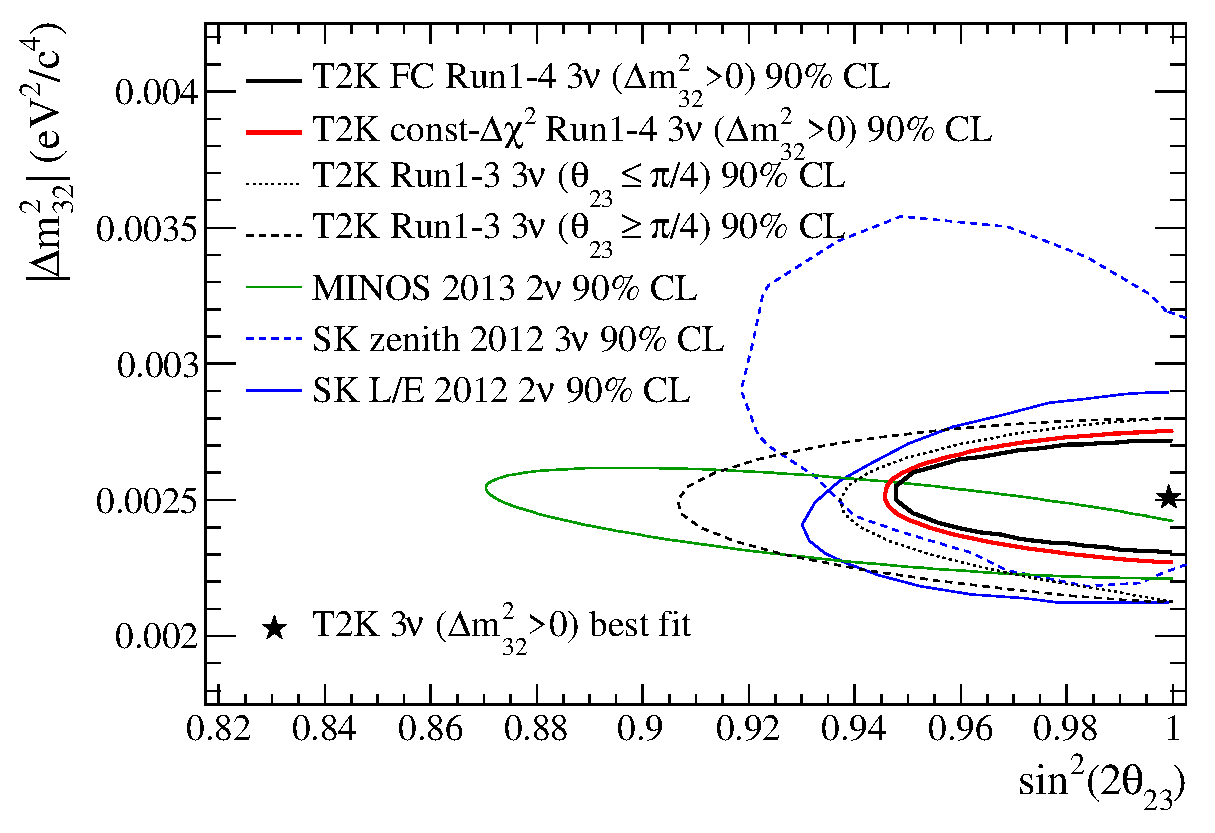
\includegraphics[width=30pc]{./images/data_fit/fc/contour_compare_constdchisqfc_external_sinsq2theta23}
  \caption {
    Comparison between 90\% CL allowed regions 
    from MINOS \cite{MINOS2013}, SuperK atmospherics \cite{SKAtm2012}, T2K Run 1+2+3 \cite{T2KRun123Disapp},
    and the 90\% CL region obtained from the {\em VALOR} fit of the Run 1+2+3+4 dataset.
    Contours obtained using both the constant-$\Delta\chi^2$ and Feldman-Cousins methods are shown.
    The normal mass hierarchy is assumed for all results.
  }
  \label{fig:results_compare_FC_constdchisq_external_sinsqtheta23}
\end{figure*}

% ......................
% 
% Comparison with sensitivity
% 
\begin{figure*}[htb]
  \center
  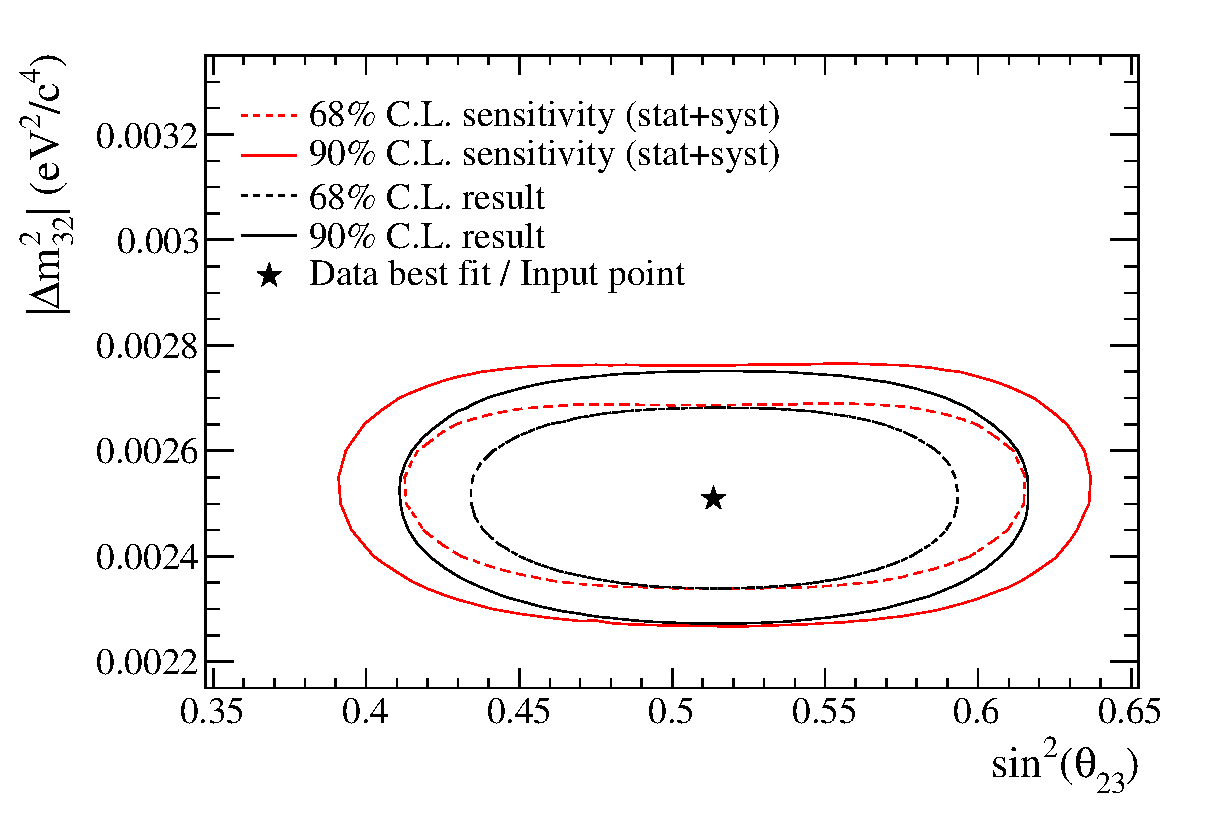
\includegraphics[width=30pc]{./images/data_fit/sensitivity/sensitivity_normal}
  \caption {
    Comparison between the 68\% CL and 90\% CL allowed regions using the constant-$\Delta\chi^2$ 
    method from the fit of the Run 1+2+3+4 dataset
    and the results of
    % sensitivity studies
    a sensitivity study
    at the best-fit point for Run 1+2+3+4
    for
    %both statistical-only and
    statistical+systematic MC toys.
    The normal mass hierarchy is assumed.
  }
  \label{fig:results_compare_constdchisq_sensitivity_normal}
\end{figure*}

% ......................
% 
% Run 1+2+3+4 vs Run 1+2+3 vs Run 4
% 
\begin{figure*}[htb]
  \center
  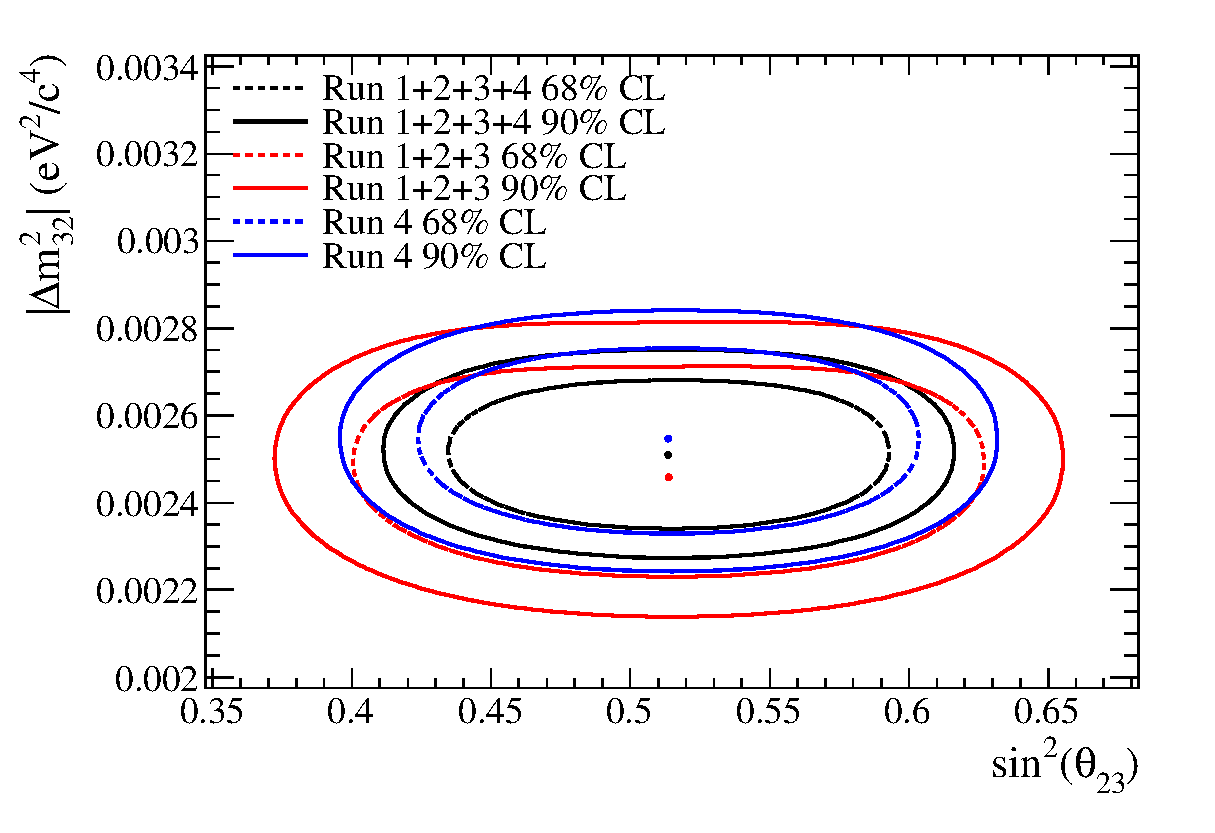
\includegraphics[width=30pc]{./images/data_fit/compare/contours_run1-4_nuis4_sepruns}
  \caption {
  Comparison between the 68\% CL and 90\% CL allowed regions obtained from separate
  analyses to the Run 1+2+3+4, Run 1+2+3 and Run 4 datasets.
  All contours shown were calculated with the constant-$\Delta\chi^2$ method.
  The normal mass hierarchy is assumed.
}
  \label{fig:results_compare_runs}
\end{figure*}


% \clearpage



% Summary and acknowledgements
\clearpage

% --------------------------------------------------------------------------------------------

\section {Summary}
\label{sec:summary}

In this technical note,
we have presented the results of a 3-flavour $\nu_{\mu}$-disappearance analysis,
performed by the {\em VALOR} group,
on the combined Run1+2+3+4 (6.5700$\times$10$^{20}$ POT) dataset.
This analysis is an update of the work presented in
Refs. \cite{OurRun1DisappAnalysis}, 
\cite{OurRun12DisappAnalysis}, 
\cite{OurRun12DisappAnalysis3Flavour},
\cite{OurRun123DisappAnalysis3Flavour} and 
\cite{OurRun1234aDisappAnalysis3Flavour}
with improved methods and an enlarged dataset.

This analysis predicts \NskNoOscExpectation $\pm$ \NskNoOscExpectationError (syst)
1 $\mu$-like ring events in SuperK in the absence of any oscillation,
but only \NskObserved were observed. The observed deficit has a strong energy dependence;
the ratio of observed to expected, under the no-oscillation hypothesis, is
$\sim$\NskNoOscRatioLow\% $<$ 0.5 GeV,
$\sim$\NskNoOscRatioMid\% between 0.5 and 1 GeV and
$\sim$\NskNoOscRatioHig\% $>$ 1 GeV.

A $\nu_{\mu}$-disappearance analysis was performed
in a framework of 3-flavour oscillations including matter effects in constant-density matter.
In this analysis, 41 neutrino flux, neutrino cross section,
efficiency, energy scale, initial-state nuclear environment and final-state rescattering,
and oscillation parameter systematics were taken into account. The oscillation parameters 
$\sin^{2}\theta_{12}$, $\sin^{2}\theta_{13}$, $\Delta m^{2}_{21}$ and $\delta_{CP}$ were 
also treated as nuisance parameters. 
The observed reconstructed energy spectrum of 1 $\mu$-like ring events was fitted,
and separate fits were made for the normal and the inverted mass hierarchies. In these fits,
$\sin^{2}\theta_{23}$ and either $|\Delta m^{2}_{32}|$ (normal hierarchy) or $|\Delta m^{2}_{31}|$ (inverted hierarchy)
were allowed to float.
The oscillation parameters $\sin^{2}\theta_{12}$, $\sin^{2}\theta_{13}$, $\Delta m^{2}_{21}$ and $\delta_{CP}$
and all 41 systematic parameters considered in this analysis were also allowed to float in the fits.

The 3-flavour $\nu_{\mu}$-disappearance fit of the combined Run 1+2+3+4 dataset,
assuming the normal mass hierarchy,
gives
\resultNormalDmsq and \resultNormalMixing
as the best-fit values (p-value = \resultNormalPvalue).
Assuming the inverted mass hierarchy, the fit yields
\resultInvertedDmsq and \resultInvertedMixing
as the best-fit values (p-value = \resultInvertedPvalue).

Confidence regions in the parameter spaces $\sin^{2}\theta_{23}$ - $|\Delta m^{2}_{32}|$ (normal hierarchy) and
$\sin^{2}\theta_{23}$ - $|\Delta m^{2}_{31}|$ (inverted hierarchy)
have been shown using both the constant-$\Delta\chi^2$ method and the method of Feldman and Cousins.
Using the new procedure described in Sec.\ \ref{sec:contour_construction}, the 68\% (90\%) confidence intervals 
in $\sin^{2}\theta_{23}$ and either $|\Delta m^{2}_{32}|$ (normal hierarchy) or $|\Delta m^{2}_{31}|$ (inverted hierarchy) 
can be summarized as
% This is 1D FC
\resultNormalMixingOneSigmaFCLo\xspace(\resultNormalMixingTwoSigmaFCLo)
$< \sin^{2}\theta_{23} <$
\resultNormalMixingOneSigmaFCHi\xspace(\resultNormalMixingTwoSigmaFCHi)
and
\resultNormalDmsqOneSigmaFCLo$\times$10$^{-3}$ (\resultNormalDmsqTwoSigmaFCLo$\times$10$^{-3}$) eV$^{2}$/c$^{4}$
$< |\Delta m^{2}_{32}| < $
\resultNormalDmsqOneSigmaFCHi$\times$10$^{-3}$ (\resultNormalDmsqTwoSigmaFCHi$\times$10$^{-3}$) eV$^{2}$/c$^{4}$
for the normal mass hierarchy,
and
\resultInvertedMixingOneSigmaFCLo\xspace(\resultInvertedMixingTwoSigmaFCLo)
$< \sin^{2}\theta_{23} <$
\resultInvertedMixingOneSigmaFCHi\xspace(\resultInvertedMixingTwoSigmaFCHi)
and
\resultInvertedDmsqOneSigmaFCLo$\times$10$^{-3}$ (\resultInvertedDmsqTwoSigmaFCLo$\times$10$^{-3}$) eV$^{2}$/c$^{4}$
$< |\Delta m^{2}_{31}| < $
\resultInvertedDmsqOneSigmaFCHi$\times$10$^{-3}$ (\resultInvertedDmsqTwoSigmaFCHi$\times$10$^{-3}$) eV$^{2}$/c$^{4}$
for the inverted mass hierarchy.
% % This is const dchisq
% \resultNormalMixingOneSigmaLo\xspace(\resultNormalMixingTwoSigmaLo)
% $< \sin^{2}\theta_{23} <$
% \resultNormalMixingOneSigmaHi\xspace(\resultNormalMixingTwoSigmaHi)
% and
% \resultNormalDmsqOneSigmaLo$\times$10$^{-3}$ (\resultNormalDmsqTwoSigmaLo$\times$10$^{-3}$) eV$^{2}$/c$^{4}$
% $< |\Delta m^{2}_{32}| < $
% \resultNormalDmsqOneSigmaHi$\times$10$^{-3}$ (\resultNormalDmsqTwoSigmaHi$\times$10$^{-3}$) eV$^{2}$/c$^{4}$
% for the normal mass hierarchy,
% and
% \resultInvertedMixingOneSigmaLo\xspace(\resultInvertedMixingTwoSigmaLo)
% $< \sin^{2}\theta_{23} <$
% \resultInvertedMixingOneSigmaHi\xspace(\resultInvertedMixingTwoSigmaHi)
% and
% \resultInvertedDmsqOneSigmaLo$\times$10$^{-3}$ (\resultInvertedDmsqTwoSigmaLo$\times$10$^{-3}$) eV$^{2}$/c$^{4}$
% $< |\Delta m^{2}_{31}| < $
% \resultInvertedDmsqOneSigmaHi$\times$10$^{-3}$ (\resultInvertedDmsqTwoSigmaHi$\times$10$^{-3}$) eV$^{2}$/c$^{4}$
% for the inverted mass hierarchy.

%Numerous comparisons have been made of the best-fit values and spectra 
%for different running periods.
Comparisons have been presented of the confidence regions obtained using different construction methods.
%and from fits to different datasets.
Finally, comparisons of our contours with
recent measurements from MINOS and SuperK
and the expected T2K sensitivity 
for 6.570$\times$10$^{20}$ POT
have also been made. 



% References
%
% References
%

\begin{thebibliography}{9}

%
% Our previous analyses
%
\bibitem{OurRun1DisappAnalysis}
   C.Andreopoulos, T.Dealtry, J.Dobson, N.Grant, M.Haigh, J.Ilic, G.Pearce and A.Weber,
   T2K 3.23$\times10^{19}$-POT Muon-Neutrino Disappearance Analysis,
   T2K-TN-036(v4),\\
   http://www.t2k.org/docs/technotes/036
\bibitem{OurRun12DisappAnalysis}
   C.Andreopoulos, T.Dealtry, J.Dobson, N.Grant, M.Haigh, J.Ilic, G.Pearce and A.Weber,
   T2K 1.431$\times10^{20}$-POT Muon-Neutrino Disappearance Analysis
   T2K-TN-064(v3),\\
   http://www.t2k.org/docs/technotes/064
\bibitem{OurRun12DisappAnalysis3Flavour}
   C.Andreopoulos, T.Dealtry, L.Escudero, N.Grant and A.Weber,
   T2K 1.431$\times10^{20}$-POT 3-Flavour Muon-Neutrino Disappearance Analysis
   T2K-TN-087(v1),\\
   http://www.t2k.org/docs/technotes/087
\bibitem{OurRun123DisappAnalysis3Flavour}
   C.Andreopoulos, T.Dealtry, L.Escudero, N.Grant and A.Weber,
   T2K 3.010$\times10^{20}$-POT 3-Flavour Muon-Neutrino Disappearance Analysis
   T2K-TN-141(v10),\\
   http://www.t2k.org/docs/technotes/141
\bibitem{OurRun1234aDisappAnalysis3Flavour}
   C.Andreopoulos, T.Dealtry, L.Escudero, N.Grant and A.Weber,
   T2K 6.3933$\times10^{20}$-POT 3-Flavour Muon-Neutrino Disappearance Analysis
   T2K-TN-155(v2),\\
   http://www.t2k.org/docs/technotes/155
\bibitem{OurRun123JointOscillationAnalysis}
   C.Andreopoulos et al.,
   T2K 3.010$\times10^{20}$-POT Joint 3-Flavour Oscillation Analysis
   T2K-TN-154(v3),\\
   http://www.t2k.org/docs/technotes/154

%
% Supplementary material to this analysis
%
\bibitem{OurRun1234DisappAnalysisSupplement}
  C.Andreopoulos, T.Dealtry, L.Escudero and N.Grant,
  T2K 6.5700$\times10^{20}$-POT 3-Flavour Muon-Neutrino Disappearance Analysis:
  Supplementary material on the effect of systematics,
  T2K-TN-183 supplement,\\
  http://www.t2k.org/docs/technotes/183

%
% Our previous published analyses
%
\bibitem{T2KRun12Disapp}
   T2K Collaboration (K.Abe et al.), 
   First Muon-Neutrino Disappearance Study with an Off-Axis Beam,
   Phys.Rev.D85:031103, 2012; arXiv:1201.1386
\bibitem{T2KRun123Disapp}
  T2K Collaboration (K.Abe et al.),
  Measurement of Neutrino Oscillation Parameters from Muon Neutrino Disappearance with an Off-axis Beam,
  arXiv:1308.0465 [hep-ex], 2013.
  
%
% Official 2012 analysis inputs and software packages
%
\bibitem{Neut:ActaP}
  Y.Hayato, A neutrino interaction simulation program library NEUT,
  Acta Phys.Polon.B40:2477-2489,2009.
\bibitem{FluxTuning}
   Beam WG, Flux tuning (11b v3.2), http://www.t2k.org/beam/NuFlux/FluxRelease/11brelease/11btuned-v3.2
\bibitem{SuperkErrors}
   M.Otani and J.Kameda,
   Super-K events and Updated systematic errors for $\nu_\mu$ disappearance analysis with T2K 1.431$\times10^{20}$ POT
   T2K-TN-065(v6),
   http://www.t2k.org/docs/technotes/065
\bibitem{NEUTnuclear}
  P. de Perio et al.,
  NEUT nuclear effects (FSI)
  T2K-TN-033(v2.0),
  http://www.t2k.org/docs/technotes/033
\bibitem{NIWGErr}
  P. de Perio et al.,
  Cross section parameters for the 2012a oscillation analysis
  T2K-TN-108(v1.3),
  http://www.t2k.org/docs/technotes/108
\bibitem{MoreNIWGErr113}
  P. de Perio et al.,
  Implementation of the NIWG cross-section parametrization,
  T2K-TN-113(v1.2) 
\bibitem{NIWGNuBarErr}
  Y.Hayato, K.McFarland, and M.Wascko (Private communication) 
% \bibitem{BANFF}
%   P. de Perio et al.,
%   Constraining the Flux and Cross Section Models with Data from the
%   ND280 Detector for the 2012a Oscillation Analysis,
%   T2K-TN-106(v8.0)
%   http://www.t2k.org/docs/technotes/106
\bibitem{SI}
  P. de Perio et al.,
  Pion Hadronic Secondary Interactions in Super-Kamiokande,
  T2K-TN-105(v1.1)
  http://www.t2k.org/docs/technotes/105
\bibitem{OldDisappSuperK}
  Y. Ashie et al., Phys. Rev. Lett. 93, 101801 (2004);
  Y. Ashie et al., Phys. Rev. D71, 112005 (2005); 
  J. Hosaka et al., Phys. Rev. D 74, 032002 (2006).
\bibitem{FluxTuningHistograms}
  Beam group,
  http://www.t2k.org/beam/NuFlux/FluxRelease/11arelease/11atuned-v2.3.
% \bibitem{1overMAQE2}
%   M. Hartz,
%   BANFF Fit Update for the 2012 Disappearance Analyses,
%   http://www.t2k.org/asg/meeting/20121015/banffinputsdisapp/view.

%
% Official 2013 inputs
%

\bibitem{ND280Inputs}
  M. Wilking,
  Status of the 2013 ND280 $\nu_{\mu}$ analysis,\\
  http://www.t2k.org/asg/meeting/20130411/nd280numustatus/view.
\bibitem{BANFF2013}
  M. Hartz, A. Kaboth, and K. Mahn,
  Constraining the Flux and Cross Section Models with Data from the
  ND280 Detector for the 2013 Oscillation Analysis,
  T2K-TN-166(v3.0)
  http://www.t2k.org/docs/technotes/166.
\bibitem{SuperkErrors2013}
   J. Kameda,
   Updated study of the systematic error in $\nu_{\mu}$ disappearance analysis from Super-Kamiokande,
   T2K-TN-159(v2),
   http://www.t2k.org/docs/technotes/159.
\bibitem{SuperkEScale2013}
   J. Hignight et al.,
   Super-Kamiokande events and data quality studies for T2K Run4
   T2K-TN-148(v2r3),
   http://www.t2k.org/docs/technotes/148.

%
% 
%

\bibitem{KDIRun1234DisappAnalysis}
  T. Wongjirad, A. Minamino and J. Kameda,
  Muon neutrino disappearance analysis with T2K 6.57 $\times$ 10$^{20}$ POT data,
  T2K-TN-164(v4),
  http://www.t2k.org/docs/technotes/164
\bibitem{2013nueptheta}
  C. Bronner et al.,
  Run1-4 p-theta electron neutrino appearance analysis,
  T2K-TN-161(v2.6),
  http://www.t2k.org/docs/technotes/161
\bibitem{2013nuenergy}
  Y. Nishimura, J. Hignight, and S. Nakayama
  $\nu_e$ appearance analysis of RUN1-4 data with neutrino energy spectrum,
  T2K-TN-162(v2.2),
  http://www.t2k.org/docs/technotes/162
%
% External papers relevant to official inputs
%
\bibitem{NA61T2K}
  N Abgrall et al. Measurements of Cross Sections and Charged Pion Spectra in Proton-Carbon Interactions
  at 31 GeV/c. Phys.Rev., C84:034604, 2011;
  N. Abgrall et al. Measurement of production properties of positively charged kaons in proton-carbon
  interactions at 31 GeV/c. arXiv:hep-ex/1112.0150, 2011.
%
% PDG-2012 
%
\bibitem{PDG2012}
  J. Beringer et al. (Particle Data Group), Phys. Rev. D86, 010001 (2012)
%
% Talks by VALOR group members referenced in the text
%
\bibitem{Lorena}
  Lorena Escudero Sanchez for the {\em VALOR} group, 
  http://www.t2k.org/asg/oagroup/meeting/20121219/VaLOR%202012%20joint%20OA%20report/view
\bibitem{Tom1overMaQE2}
  Tom Dealtry for the {\em VALOR} group,
  http://www.t2k.org/asg/meeting/2012/20121015/valornumudisapp/view
%
% Statistics etc
%
\bibitem{StatAnalysisCowan} 
  G. Cowan (1998) Statistical data analysis, 
  Oxford University Press, ISBN 0-19-850155-2.
\bibitem{Minuit}
  F.James, M.Roos, Minuit: A System for Function Minimization and Analysis of the 
  Parameter Errors and Correlations, Comput.Phys.Commun. 10:343 (1975)
%\bibitem{NumRecipCholesky}
%  Numerical Recipes: The art of scientific computing, 
%  Cambridge University Press, 3rd Edition, ISBN 978-0-521-88068-0, pp. 100-102.
%\bibitem{RevPartPhysStat}
%  C. Amsler et al. (Particle Data Group),
%  Review of Particle Physics, Phys.Lett.B667:1,2008 
\bibitem{FeldmanCousins}
  G.J. Feldman and R.D. Cousins,
  A Unified approach to the classical statistical analysis of small signals,
  Phys.Rev.D57:3873-3889,1998; physics/9711021
\bibitem{CousinsHighland}
  R.D. Cousins and V.L.Highland, 
  Nucl.Instr. and Meth. A320:331035, 1992.
\bibitem{NickPvalue}
 N.Grant for the {\em VALOR} group,
 http://www.t2k.org/asg/meeting/2011/20111124/pvalues/view
\bibitem{KarlenPvalue}
 D.Karlen,
 p-values, distributions and low statistics,
 http://www.t2k.org/asg/oagroup/meeting/20120416/lowstat/view
%
% Numu contour committe report
%
\bibitem{T2KNuMuContourCom}
  K. McFarland for the T2K $\nu_{\mu}$-disappearance contour committee 
  (C.Andreopoulos, N.Grant, J.Kameda, D.Karlen, E.Kearns, K.McFarland, M.Otani, M.Zito)
  Report to ASG conveners meeting, 17 May 2011,
  http://www.t2k.org/asg/contour/ASG-Conveners-Report/view
%
% MINOS, SK atm. "23"-sector oscillation analyses
%
\bibitem{MINOS2012}
  R.Nichol,
  Talk at Neutrino 2012
\bibitem{MINOS2013}
  P. Adamson, et al.,
  Measurement of Neutrino and Antineutrino Oscillations Using Beam and Atmospheric Data in MINOS,
  arXiv:1304.6335 [hep-ex], 2013
\bibitem{MINOS2013sinsqtheta}
  A. Radovic,
  Talk at DPF 2013
\bibitem{SKAtm2012}
  Y. Itow,
  Recent results in atmospheric neutrino oscillations in the light of large $\theta_{13}$,
  Nucl. Phys. B (Proc. Suppl.) 235 79 (2013).

% 
% Experiment-specific theta13, theta12, and dmsq12 refs
%
%\bibitem{Kamland}
%  S. Abe et al.,
%  Precision measurements of neutrino oscillation parameters with KamLAND
%  Phys.Rev.Lett.100:221803,2008
%\bibitem{DayaBay}
%  F.P. An et al.,
%  Observation of electron-antineutrino disappearance at Daya Bay
%  Phys.Rev.Lett.108:171803,2012
%\bibitem{Reno}
%  J.K. Ahn et al.,
%  Observation of reactor electron antineutrinos disappearance in the Reno experiment
%  Phys.Rev.Lett.108:191802,2012
%
% Global oscillation analyses
%
\bibitem{FogliLisi}
  G.L.Fogli, E.Lisi et~al.,
  Evidence of theta(13)$>$0 from global neutrino data analysis,
  Phys.Rev.D84:053007, 2011; arXiv:1106.6028 [hep-ph]
\bibitem{GonzalezGarcia}
 M.C.Gonzalez-Garcia, M.Maltoni, J.Salvado and T.Schwetz,
 Global fit to three neutrino mixing: critical look at present precision,
 arXiv:1209.3023 [hep-ph]
%\bibitem{ockham}
%  "Ockham's razor", Encyclopedia Britannica
%  http://www.britannica.com/EBchecked/topic/424706/Ockhams-razor
%
% 3-flavour oscillation probability formulas etc
%
%\bibitem{kayser2005}
%  B. Kayser (2005), Neutrino physics, hep-ph 0506165
%\bibitem{giunti}
%  C Giunti and C.W. Kim (2007) Fundamentals of neutrino physics and astrophysics, Oxford Uninversity Press
%\bibitem{pdgreview}
%  K. Nakamura and S.T. Petcov (2010) Neutrino mass, mixing and oscillations,
%  http://pdg.lbl.gov/2010/reviews/rpp2010-rev-neutrino-mixing.pdf
%\bibitem{kopp}
%  J. Kopp (2006), Efficient numerical diagonalisation of Hermitian 3x3 matrices, arXiv:physics/0610206
%
% Other 3-flavour oscillation probability packages
%
%\bibitem{sloan}
%  T. Sloan, private communication (June-July 2011)
\bibitem{Prob3}
 Prob3++ 3-flavour oscillation probability software,
 http://www.phy.duke.edu/~raw22/public/Prob3++/

\end{thebibliography}




% Appendices
% \clearpage
% \appendix
% \addappheadtotoc

\clearpage

\end{document}

